\documentclass[12pt,oneside]{book}

% \usepackage{natbib}
\usepackage[
    natbib=true,
    style=numeric,
    sorting=none]{biblatex}
\addbibresource{references.bib}

% packages
\usepackage{xspace}
\usepackage{textcase}
\usepackage{dcolumn}
\usepackage{longtable}
\usepackage[version=4]{mhchem}
\usepackage{hyperref}
\usepackage{cleveref}
\usepackage{booktabs}
\usepackage{multirow}
\usepackage{multicol}
\usepackage{wasysym}
\usepackage{graphics}
\usepackage{graphicx}
\usepackage{amsmath}
\usepackage{amsthm}
\usepackage{amssymb}
\usepackage{footnote}
\usepackage{layout}
\usepackage[utf8]{inputenc}
\usepackage{siunitx}
\usepackage{mathtools}


% define the margins of the document
\usepackage{geometry}
\geometry{
    left = 1.5cm,
    right = 1.5cm,
    top = 2cm,
    bottom = 2cm
}

% asterix command ([1] => *)
% \usepackage[symbol]{footmisc}
\renewcommand{\thefootnote}{\fnsymbol{footnote}}

% overbar command
\usepackage{amsfonts}
\newcommand{\overbar}[1]{\mkern 2.5mu\overline{\mkern-2.5mu#1\mkern-2.5mu}\mkern 2.5mu}

%%%%%%%%%%%%%%%%% STYLISTIC HEADINGS %%%%%%%%%%%%%%%%%%%%%%%
\pagestyle{headings}
% Note that the line below could be modified to suit a
% particular system since the "geometry" package behaves
% differently in Unix, Windows and Mac, especially for the
% top margins.
% Adjust the parameter "top" (measuring the height of the
% space allocated to a header) and "headsep" (measuring
% the distance from the bottom of the header to the
% first line of text.
% \usepackage[top=1.3in,left=1.5in,bottom=1in,right=1in,headsep=0.5in]{geometry}

\usepackage{setspace}
\onehalfspacing
%\doublespacing

% Headers and footers for thesis
\usepackage{fancyhdr}

\markboth{}{}
\newcommand\startchapter[1]{\chapter{#1}\thispagestyle{myheadings}}
\newcommand\startappendix[1]{\chapter{#1}\thispagestyle{myheadings}}
\newcommand\startfirstchapter[1]{\chapter{#1}}

% Manual addition of section to Table of Contents
\newcommand\TOCadd[1]{\newpage\phantomsection\addcontentsline{toc}{chapter}{#1}}

% Float Customization
\renewcommand{\floatpagefraction}{0.01}

% Customization of Tables of Contents and List of Figures/Tables
\usepackage{tocloft}
\renewcommand\cfttabpresnum{Table\ }
\renewcommand\cfttabnumwidth{0.75in}
\renewcommand\cftfigpresnum{Figure\ }
\renewcommand\cftfignumwidth{0.80in}
\newcommand{\HRule}{\rule{\linewidth}{0.5mm}}

%%%%%%%%%%%%%%%%%%%% DEFINE COMMANDS %%%%%%%%%%%%%%%%%%%%%%%%
\newcommand{\beginsupplement}{%
        \setcounter{table}{0}
        \renewcommand{\thetable}{S\arabic{table}}%
        \setcounter{figure}{0}
        \renewcommand{\thefigure}{S\arabic{figure}}%
        \setcounter{equation}{0}
        \renewcommand{\theequation}{S\arabic{equation}}%
     }
\renewcommand{\thefootnote}{\roman{footnote}}


\begin{document}

% Front Matter
\input frontmatter/fm

\newpage

% demonstrated chapters with suggestions and tips
% \startchapter{The Problem to be Solved}
\label{chapter:problem}

\newlength{\savedunitlength}
\setlength{\unitlength}{2em}

Here is where you tell me what is the problem you have been working on for the past few months (or years). I want all the details and you should not be timid about being too tutorial, except that you do not want to cross the line towards writing a textbook. However consider carefully that \textit{communication} implies conveying ideas to other people, while \textit{effective communication} occurs when your message is clearly understood. Remember that your audience must understand your message before they can agree with you.

Ask yourself:
\textit{who is your audience?} You might think of your supervisor who knows everything and you want to impress with your knowledge. I think instead of the graduate students who will be reading this thesis which is, after all, a property of the university. It is published as a university technical report so that others may learn by reading it. Then teach them! Be a bit tutorial. Even the expert external examiner will be impressed by your clarity of exposition if he or she does not need to read paragraphs twice in order to understand - something which people with PhDs and big egos find particularly irritating.

On the other hand, do not go too far and give trivial definitions from concepts learned in a 3rd year undergraduate courses, else you might find yourself in trouble when having to remember the details during an oral examination.

My approach is to put everything necessary to make clarity for
the problem the main goal of this chapter, assuming an intelligent and well prepared reader who already has a Bachelor degree in an appropriate subject.

Once I understand the problem clearly and its nuances (it may not be what I expected after all), I also need to know why the problem is important, what its impact is and what its application, if any. Here you are free to elaborate and write as much as you think is necessary to avoid the examination doubt that you have a brilliant new solution to a trivial and unimportant issue.

I suggest reading various books on how to do research and set up problems. The best for me was "The Craft of Research" by Wayne Booth \cite{booth1}, which can be found in the main library at Q180.55 M4B66. From there I have transferred to my writing a fairly simple structure for talking about the topic of the research, with the question to be asked and its motivation and significance. It goes as follows:
\begin{enumerate}
\item {\textit{I am trying to learn about (working on, studying...)}}
\item {\textit{because I want to find out....}}
\item {\textit{in order to understand...}}
\end{enumerate}

Another way of looking at this is to ask the
\textit{what}, \textit{why} and \textit{where}, starting from a \textit{setting} of the problem with a first point A, stating what the \textit{goal} is at point B and having an \textit{action link} between the two which will encompass your new solution. As surprising as this may be to some of you, I found reading a book from Microsoft very useful: "Beyond Bullet Points: Using Microsoft Office PowerPoint 2007 to Create Presentations That Inform" \cite {atkin}. The goal of the book is to improve presentations with Power Point, but there is a lot that can be transferred towards \textit{effective communication} for a thesis.

In summary, my view of the second chapter on
\textit{"The Problem to be solved"} is as follows:
\begin{enumerate}
\item {\textit{Not} all the background and definitions (boring!) - use instead just-in-time explanations as needed in every context as it comes up;}
\item {Motivation in depth;}
\item {Tutorial high level explanation, where it is important to choose the right pitch: who is the audience? who are you teaching here?}
\item {Make it exciting, make it current, make it important - why do I want to keep reading?}
\item {Should you list here the solutions from other researchers? I think not, list instead the different facets of the problems that other researchers have attacked.}
\item {A taxonomy can be extremely useful to place your problem and its particular special features within the perfect context of the overall area, as you need to make sure that the reader understands perfectly what you are trying to solve.}
\end{enumerate}


\setlength{\unitlength}{\savedunitlength}

% \startchapter{Conclusions}
\label{concl}

My first rule for this chapter is to avoid finishing it with a section talking about future work. It may seem logical, yet it also appears to give a list of all items which remain undone! It is not the best way psychologically.

This chapter should contain a mirror of the introduction, where a summary of the \textit{extraordinary} new results and their wonderful attributes should be stated first, followed by an executive summary of how this new solution was arrived at. Consider the practical fact that this chapter will be read quickly at the beginning of a review (thus it needs to provide a strong impact) and then again in depth at the very end, perhaps a few days after the details of the previous 3 chapters have been somehow forgotten. Reinforcement of the positive is the key strategy here, without of course blowing hot air.

One other consideration is that some people like to join the chapter containing the analysis with the only with conclusions. This can indeed work very well in certain topics.

Finally, the conclusions do not appear only in this chapter. This sample mini thesis lacks a feature which I regard as absolutely necessary, namely a short paragraph at the end of each chapter giving a brief summary of what was presented together with a one sentence preview as to what might expect the connection to be with the next chapter(s). You are writing a story, the \textit{story of your wonderful research work}. A story needs a line connecting all its parts and you are responsible for these linkages.


% chapters
\newpage
\startfirstchapter{Introduction}
\label{chapter:introduction}




\input chapters/1/sec_intro
\input chapters/1/sec_review
%\pagebreak
\section{My Claims}
Something must be new in this work, no matter how small, since you are getting a graduate degree for it! Tell me about it clearly and succintly right now, just as you did in the abstract. Make an impact here. How about something like the following box:

I make \textit{four} claims which
my dissertation validates:
\\

\framebox{%
\parbox{5in}{
	My new algorithm to solve the problem of doing nothing include these important new features whose practical applicability can be proved both formally and empirically:
	\begin{enumerate}
	\item first feature;
	\item second feature;
	\item everything is much easier to understand, and therefore, easier to implement correctly.
	\end{enumerate}
}}
\\

\noindent Claim 1 and claim 2 are \textit{quantitative} - they will be proven by experiment.

\noindent Claim 3 is \textit{qualitative} - they will be demonstrated by argument.

\subsection{The Importance of My Claims}

Some very important positive consequences
arise from the validation of the above claims.
It is these consequences that comprise a significant
positive contribution to research in the field
of whatever the field is.
\\

\noindent Claim 1 implies that:
\begin{enumerate}
\item{Something profound which applies to:
	\begin{itemize}
	\item {something excellent;}
	\item {something important.}
	\end{itemize}}
\item{Something else just as profound.}
\end{enumerate}

\noindent Claim 2 implies that:
\begin{itemize}
\item{Repeat as above if necessary and useful.}
\end{itemize}

\noindent The consequence of claim 3 is that:
\begin{itemize}
\item{There must be something good coming out of all this work!}
\end{itemize}

\section{Agenda}

This section provides a map of the dissertation
to show the reader where and how it validates
the claims previously made. Here is where I am also presenting my own style of organization which may be totally different from what your supervisor thinks. However, trust me, this is a good solid beginning for a structure. Your supervisor may ask you to change it, but will still appreciate what you have! For each of the chapters below I also give a short summary of what the main focus should be and then I expand on it  a bit within the chapter itself.

\begin{description}
\item[\textbf{Chapter 1}] contains a statement of
the claims which will be proved by this dissertation followed by an overview of the structure of the document itself.
\item[\textbf{Chapter 2}] describes in details the open problem which is to be tackled together with its context, its impact and the overall motivation for the research overall.
\item[\textbf{Chapter 3}] gives the new research, its methodology, the algorithms involved, the new solution, the new work done. Formal proofs and arguments are made here. This is the first of the two contributions expected in a thesis for a graduate degree.
\item[\textbf{Chapter 4}] is where the experiments and the methodology for them is fully described. The first part includes all details of how the empirical side of the research has been conducted. Note that not every thesis has this empirical portion.
\item[\textbf{Chapter 5}] includes the evaluation of the data presented above and the comparisons with the work of others, to show how much better the new approach is. This is the second of the two contributions expected in a thesis for a graduate degree. Note that this part could be consolidated into the chapter above.
\item[\textbf{Chapter 6}] contains a restatement of the claims and results of the dissertation. It also enumerates avenues of future work for further development of the concept and its applications.
\end{description}

The list above is not complete. Chapter 3 actually includes a lot more, as I could not resist placing in it a few \LaTeX examples to help you along. This document is not a primer for \LaTeX, but there is no harm done in giving a little help.


\newpage
\startchapter{A one-dimensional model of scaling in Reverse Osmosis: ROSSpy}
\label{ROSSpy_chapter}

\section{Introduction}
Desalination technologies, most notably reverse osmosis (RO) \cite{Malaeb2011ReverseReview}, are imperative for meeting the 6th UN Sustainable Development Goal \cite{Jones2018TheOutlook} of universalizing potable freshwater. Arid Middle-Eastern countries, who are both relatively affluent and geographically prone to water scarcity, are embracing RO desalination to satisfy domestic water needs; Israel, for example, supplies $\frac{3}{4}$ of its domestic water from desalination \cite{Shemer2017SustainableImpact} and Saudi Arabia is responsible for $\approx 22\%$ of global water desalination \cite{Council2021WaterPrivatization}. RO is the most economical desalination technology \cite{Karime2008ROPlant,Hafez2003EconomicsStudy}, however, it remains insufficiently efficient and economical for the low-resource communities. RO efficiency can be improved \cite{Elimelech2011TheEnvironment,Semiat2008EnergyProcesses} a) with energy recovery devices \cite{Amy2017Membrane-basedProspects}, that allow RO to approach the thermodynamic limit of desalinating seawater \cite{Zarzo2018DesalinationFuture}, and b) by mitigating membrane fouling such as scaling \cite{Warsinger2015ScalingReview,Khan2013SourceSea,Tang2014FoulingPlant,Shmulevsky2017AnalysisMembranes}, where minerals deposit upon the membrane surface and decrease membrane permeability such that greater applied pressures and energy usage are required to maintain a permeate flux over time. Scaling occurs mechanistically either through homogeneous precipitation from the highly concentrated brine byproduct of RO \cite{VanWagner2009EffectPerformance,Belfer1998SurfaceMembranes} -- which is itself hazardous \cite{Fernandez-torquemada2012DispersionPlants,Clemens1955ToxicityWells,Allen1989ApparatusBrine,Munn1989EffectCrops} but can be processed into useful salts \cite{Allen1954ProcessBrine,Fenton1992DesalinationWells} in zero-liquid waste management systems \cite{Jeppesen2009MetalConcentrate,Mavukkandy2019BrineGeneration} or used in mixing-entropy batteries \cite{Ye2019Charge-FreeMaterials} -- or through heterogeneous deposition upon nucleation sites on the membrane surface \cite{Karabelas2014IncipientChannels,Warsinger2018InorganicOsmosis}. The heterogeneous mechanism specifically occurs in a hyper-concentrated layer adjacent to the membrane called the concentration polarization (CP)   \cite{McCutcheon2006InfluenceOsmosis,Murthy1997EstimationModel,Gruber2011ComputationalSystems,Sablani2001ConcentrationReview,Zydney1997StagnantSystems,Li2016Three-dimensionalChannel}, which is achieved as a consequence of the no-slip boundary condition -- analogous to the capillary effect -- that prevents the CP from mixing with the bulk solution since the velocity gradient of the fluid reaches zero adjacent to the stationary filtration membrane \cite{Rapp2017Fluids}. 

Scaling, unfortunately, is experimentally elusive \cite{Hu2014Real-timeSpectroscopy,Butt1995IdentificationAutopsy,Sheikholeslami2003KineticsM}. Computational programs \cite{Giere2009IsExperimentation,Wijmans1995TheReview} may supplement experimental procedures \cite{Lenhard2007ComputerModeling,Chai2007UltrasoundModules} as a means to investigate scaling and optimize RO efficiency; however, current programs are either unspecific to RO \cite{2018ZeroPHREEQC} or focus upon other aspects of RO: e.g. plant operation \cite{DesalitechROSASoftware,Chee2018PerformanceSoftware,SysCAD2020PHREEQCUnit,Bouchareb2019ExperimentalDesalination}, permeate flux \cite{Xu2012TOUGHREACT.0,Steefel2015ReactiveSimulation}, brine geochemistry \cite{Kundu2018TechnicalTechnology}, or fluid dynamics of the CP \cite{Walker2003AssessmentReaction}. Mathematical programs \cite{Radu2014ASystems,Karabelas2019PredictionSimulator} and some with a user interface \cite{SoftwareReverseOsmosis,Strubbe2018CalibrationFull-Scale} have been developed that simulate RO scaling, however, these lack an application programming interfaces (APIs), which is essential for the broad analyses, over a continuum of variables, that could accelerate geochemical scaling research. 

We therefore developed a unique one-dimensional model that captures both the geochemistry of scaling equilibria and the reactive transport of desalination, in contrast to existing one-dimensional RO models that utilize the steady-state approximation and the solution-diffusion model \cite{Strubbe2018CalibrationFull-Scale}. This one-dimensional RO model -- similar only to the WaterTap model \cite{NAWI2021WaterTap} -- is critically amenable with PHREEQC \cite{Parkhurst2015PhreeqcRM:PHREEQC,Charlton2011ModulesLanguages}, which provides a rigorous and open-source numerical implementation of our model, similar to previous studies of scaling \cite{Mitrouli2016CalciumExperiments,Warsinger2018InorganicOsmosis} and RO \cite{Bein1993OriginBrine,Wilson1993GeochemistryFormations,Casas2012SeawaterElectrodialysis,Yan2017ReverseVelocity}. We exemplify our model through replicating experimental literature and conducting numerous sensitivity analyses across continuums of parameter values. We further developed the only, to our knowledge, open-source API of RO reactive transport (ROSSpy: RO Scaling Software in Python) based upon our model, which fulfills identified needs of a scaling software for RO research \cite{Karabelas2020ScalingTools}, where users can create, execute, process, visualize, and export simulations with predicted scale mass per membrane filtration area ($\frac{g~scale}{filtration~m^2}$) and ionic brine concentrations. Developers are encouraged to contribute to ROSSpy, which we believe is an important stride towards satisfying research needs in scaling and ultimately reducing water insecurity, especially in low-resource contexts. 

\section{Methods}

\subsection{Conceptual}

Our model represents RO desalination as a one-dimensional reactive transport process along the membrane-solution interface. The feed is represented by the single-domain model in Figure S4, where the bulk and CP solutions are aggregated into a single solution, as opposed to the more resolved dual-domain model, where the bulk and CP solutions are distinguished (Figure S5) \cite{Chen2016AssessingModel,Scruggs2019TheInterface,Greskowiak2015AUVI,Mieles2012AnalyticalSystem}. The dual-domain remains elusive within the confines of PHREEQC code (Section 6 of the Supporting Information) and moreover we demonstrate that the single-domain model is sufficient to recapitulate experimental results. Our model represents feed at the RO inlet with the Dirichlet boundary condition \cite{Moes2006ImposingMethod,Bazilevs2007WeakMechanics} -- a mathematical description of constant conditions at a model boundary -- where the influent feed is assumed to be an infinite reservoir and thus its concentration is immutable. Our model represents the RO outlet with the Cauchy boundary condition \cite{Gosses2018ExplicitModels} -- a mathematical description of dynamic conditions at a model boundary -- where the effluent concentrations dynamically depend upon desalination. A glossary of parameters and variables for the equations and calculations are provided in Table S1.


\subsection{Numerical}
The geochemistry and reactive transport components of our RO model are numerically detailed in the following sub-sections. 

\subsubsection{Permeate Flux}
The permeate flux in our model is assumed to be 100\% water, similar to other RO models \cite{Li2012OptimalDesalination}, and it is calculated as the change in moles ($\Delta \Phi_{e}$) of feed solution in any examined cell $e$. Permeate flux is proportional to the difference between feed pressure $P$ and osmotic pressure $\pi$ \cite{VanWagner2009EffectPerformance,Schock1987MassModules,Lonsdale1965TransportMembranes}
\begin{equation} \label{pressure_differential}
    \Delta \Phi_{e} ~ \alpha ~ (P - \pi),
\end{equation} 
however, these pressures are not readily measured or reported; hence, we calculate the permeate flux via two comparable methods that are elaborated in the following sub-sections.

\paragraph{Method 1: Linear permeate flux}
One method assumes that permeate flux decreases linearly along the RO module. This causes the concentration -- which is represented by the concentration factor (CF) \cite{McCaffrey1987TheHalite.,Casas2012SeawaterElectrodialysis,Kartashevsky2015PhosphateEffluents,Yan2017ReverseVelocity,Evangelista1985APlants}
\begin{equation} \label{cf_definition}
    CF = \frac{initial}{final}~,
\end{equation}
as the quotient of initial to final ionic concentrations (influent vs. effluent), solution masses, or permeate moles \cite{Casas2012SeawaterElectrodialysis,Yan2017ReverseVelocity} -- to increase exponentially along the RO module. The negative slope of permeate flux is calculated between the first cell $1$ and the last cell $n$
\begin{equation} \label{flux_slope}
    slope = \frac{(\Delta \Phi_{n}-\Delta \Phi_{1})}{n}~,
\end{equation}
where the simulated membrane-solution interface is discretized into $n$ equal fractions (cells) of the total module length $l_{module}$. The permeate fluxes in these border cells, $\Delta \Phi_{1}$ and $\Delta \Phi_{n}$, are calculated through a system of equations. One of these equations
\begin{equation} \label{average_permeate_flux}
     \overbar{\Delta \Phi}_{e} = \frac{\Delta \Phi_{module}}{n} = \frac{\Delta \Phi_{n} + \Delta \Phi_{1}}{2}
\end{equation}
equates two definitions of the average permeate flux per cell $e$: 1) $\overbar{\Delta \Phi}_{e} = \frac{\Delta \Phi_{module}}{n}$ from the total permeate flux over the module $\Delta \Phi_{module}$, and 2) $\frac{\Delta \Phi_{n} + \Delta \Phi_{1}}{2}$, as the average between the border cells. The other equation is the definition of relative pressure loss over the RO module \cite{Srivathsan2014ReverseUnsteadiness,Gu2020ModelingNetworks} ($HL ; 0\le HL\le 1$) per \cref{pressure_differential},
\begin{equation} \label{head_loss}
     \Delta \Phi_{n}= \Delta \Phi_{1}*(1-HL),
\end{equation}
which is $\approx 10\%$ \cite{Fraidenraich2009ReverseExperiment,Evangelista1985APlants,Dandavati1975HollowSystems}. The substitution of \cref{head_loss} into \cref{average_permeate_flux} -- given $HL$, $\Delta \Phi_{module}$, and $n$ -- permits calculating $\Delta \Phi_{1}$ and  $\Delta \Phi_{n}$, the flux slope of \cref{flux_slope}, and subsequently $\Delta \Phi_{e}$ from a linear expression of permeate flux per module cell
\begin{equation} \label{intermediary_permeate_flux}
    \Delta \Phi_{e} = (slope*e+\Delta \Phi_{1}).
\end{equation}
% Our permeate efficiency parameter ($PE; 0<PE<1$) applies here as means of considering module inefficiencies like preexisting fouling in the RO module that lessen the permeate flux of the system. The $PE$ scalar attenuates the total module permeate flux over the module through reducing \cref{intermediary_permeate_flux}: i.e. $\Delta \Phi_{old~module} = \Delta \Phi_{new~module}*PE$; $PE=0$ leads to $\Delta \Phi_{e}=0 ~\forall~ e$; and $PE=HL=1$ leads to $\overbar{\Delta \Phi}_{e}=\Delta \Phi_{e} ~\forall~ e$.

The calculation sequence for this permeate flux method is summarized:
\begin{enumerate}
    \item Define $HL$, $\Delta \Phi_{module}$, and $n$
    \item Calculate the permeate flux slope [\cref{flux_slope,average_permeate_flux,head_loss}]
    \item Calculate the permeate flux in each cell $e$ [\cref{intermediary_permeate_flux}]
\end{enumerate}


\paragraph{Method 2: Linear Concentration Factor}
The second method of calculating the permeate flux assumes that the CF increases linearly, which causes the permeate flux to decrease non-linearly, along the RO module. The CF slope is calculated analogously to \cref{flux_slope}:
\begin{equation} \label{average_cf_slope}
    slope_{CF} =\frac{CF_{n}-CF_1}{n}.
\end{equation}
The effluent $CF_{n}$ is the average CF of all effluent ion concentrations 
\begin{equation} \label{cf_calculation_output}
    CF_{n}=\frac{\sum_{i=1}^j(C_{i,brine})}{\sum_{i=1}^j(C_{i,feed})},
\end{equation}
where $C_{i,brine}$ is the effluent concentration and $C_{i,feed}$ is the influent concentration of ion $i$, for all $j$ ions. Defining CF from \cref{cf_definition} in terms of moles of feed solution ($\Phi$, which is assumed to be 100\% water) reveals an equation 
\begin{equation} \label{cf_cell_definition}
    CF_e=\frac{\Phi_0}{\Phi_e}=\frac{\Phi_0}{\Phi_0-\Delta \Phi_{(1,e)}}
\end{equation}
that can calculate the moles of feed at the end of an arbitrary cell $e$ ($\Phi_e$), where $\Delta \Phi_{e} = \Phi_0 - \Delta \Phi_{(1,e)}$ and $\Delta \Phi_{(1,e)}$, as the sum of permeate flux that occurred between cell $1$ and the end of cell $e$, is separately the sum
\begin{equation} \label{moles_removed_to_cell}
    \Delta \Phi_{(1,e)}=\Delta \Phi_{e}+\Delta \Phi_{(1,e-1)}
\end{equation}
of permeate flux before the start of cell $e$ ($\Delta \Phi_{(1,e-1)}=\sum_{j=1}^{e-1}(\Delta \Phi_{j})$) and the permeate flux over cell $e$ ($\Delta \Phi_{e}$). The initial moles of feed $\Phi_0$ is calculated
\begin{equation} \label{feed_mass}
    \Phi_0=V_{feed}*MW_{H_2O}*\rho_{H_2O},
\end{equation}
from the volume of the feed channel $V_{feed}$, which is the product of the module length $l_{module}$ and the cross-sectional area of the feed channel $A_{feed}$
\begin{equation} \label{feed_area}
    A_{feed}=(A_{module}-A_{permeate})*\frac{th_{feed}}{th_{unit}}~,
\end{equation}
where $A_{module}$ and $A_{permeate}$ are the cross-sectional areas of the whole module and the permeate tube, respectively, and $th_{feed}$ and $th_{unit}$ are the thicknesses of the feed channel and the repeating membrane unit in Figure S1, respectively. The linear expression for $CF_e$ 
\begin{equation} \label{cf_permeate_flux}
    CF_e=(slope_{CF})*e+CF_{0}~,
\end{equation}
is then substituted into \cref{cf_cell_definition}, with the slope from \cref{average_cf_slope}, to yield an expression for the permeate flux (a negative change in feed moles) at the end of each examined cell $e$
\begin{equation} \label{moles_removal_per_cell} 
    -\Delta \Phi_{(1,e)}=\frac{\Phi_0}{((\frac{CF_{n}-CF_{0}}{n})*e+CF_{0})}-\Phi_0~,
\end{equation}
which can be substituted into \cref{moles_removed_to_cell} with the sum of previous permeate fluxes ($\Delta \Phi_{(1,e-1)}$) to yield the permeate flux over any examined cell $e$ ($\Delta \Phi_{e}$), analogously to \cref{intermediary_permeate_flux}. Note that $\Delta \Phi_{(1,e-1)}=0$ when $e=1$, since there are no previous cells. 

The calculation sequence for this permeate flux method is summarized:
\begin{enumerate}
    \item Define the effluent CF
    \item Calculate the feed capacity of the module [\cref{feed_mass,feed_area}]
    \item Calculate the CF slope [\cref{average_cf_slope}]
    \item Calculate the permeate flux in each cell [\cref{cf_cell_definition,moles_removed_to_cell,cf_permeate_flux,moles_removal_per_cell}]
\end{enumerate}

\paragraph{Comparison of permeate flux methods}
Scaling predictions from these two permeate flux methods are juxtaposed in Figure \ref{permeate_approach}. The most significant difference is observed at the mid-point of the simulated module ($0.47 m$), where the linear CF method predicts $0.99 \frac{gram}{m^2}$ of Gypsum scale while the linear permeate flux method predicts $0.0196 \frac{gram}{m^2}$ of Gypsum scale. The linear CF method subsequently predicts subtly less scale than the linear permeate method. These different distributions are explained by the dependency of scale upon the solution CF -- where the exponential increase in CF through the linear permeate flux method causes initially less, and then eventually more, scaling than the linear CF method -- however, the scale distribution ultimately equates between these two permeate flux methods to 3 significant digits: $38.7 \frac{gram}{m^2}$. These methods are therefore believed to only subtly affect the distribution, and not the total quantity, of scale within a module. Experimental literature is not known that can verify which method better reflects physical systems. 

\subsubsection{Geochemistry}
The geochemistry of RO scaling in our model is predicated upon the kinetic rate laws and thermodynamic equilibria that define each mineral dissolution and precipitation. These chemical processes are encapsulated in the PHREEQC databases that offer different a) geochemical models, b) permissible ranges of conditions, and c) sets of potential minerals to best represent a given system. These databases are complemented with the ChemW Python package that rigorously calculates the molecular mass of each mineral (see the ChemW PyPI documentation) to permit scaling predictions in the conventional units of $\frac{g~scale}{m^2~membrane}$.

\begin{figure}
    \centering
    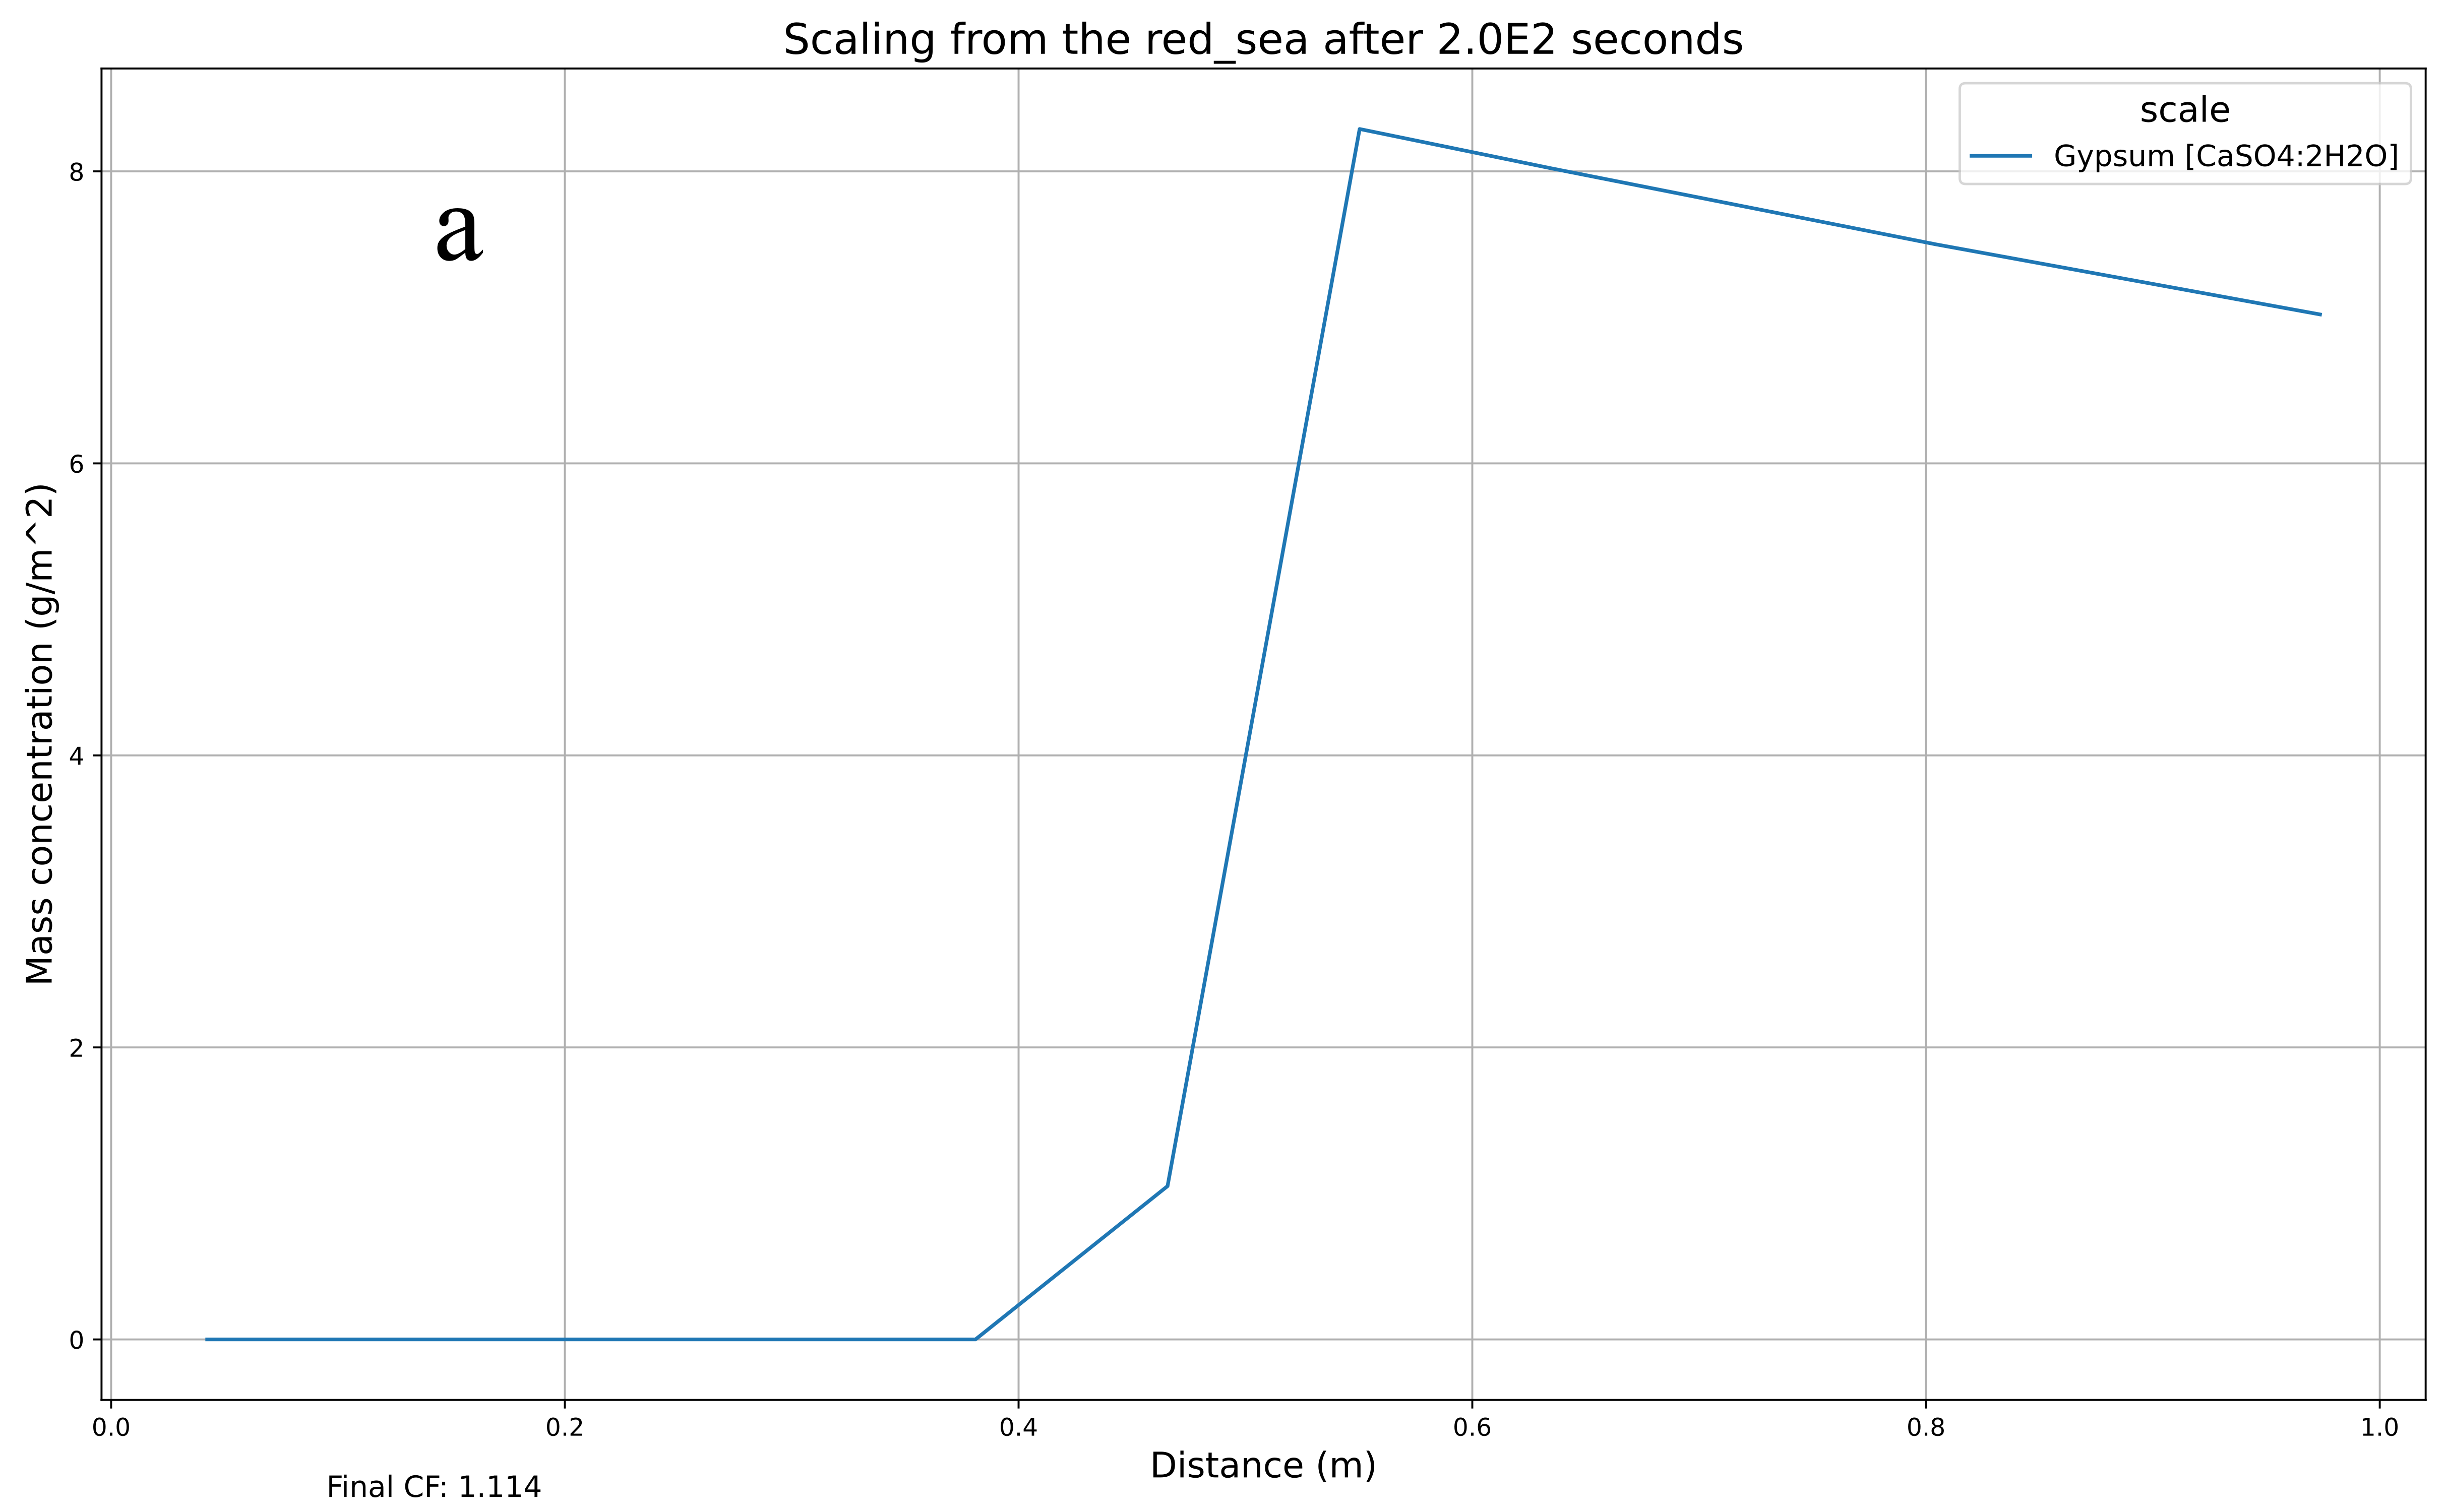
\includegraphics[width=0.9\linewidth]{images/ROSSpy/sensitivity_analyses/permeate_approach/linear_cf.png} \\ \midrule
    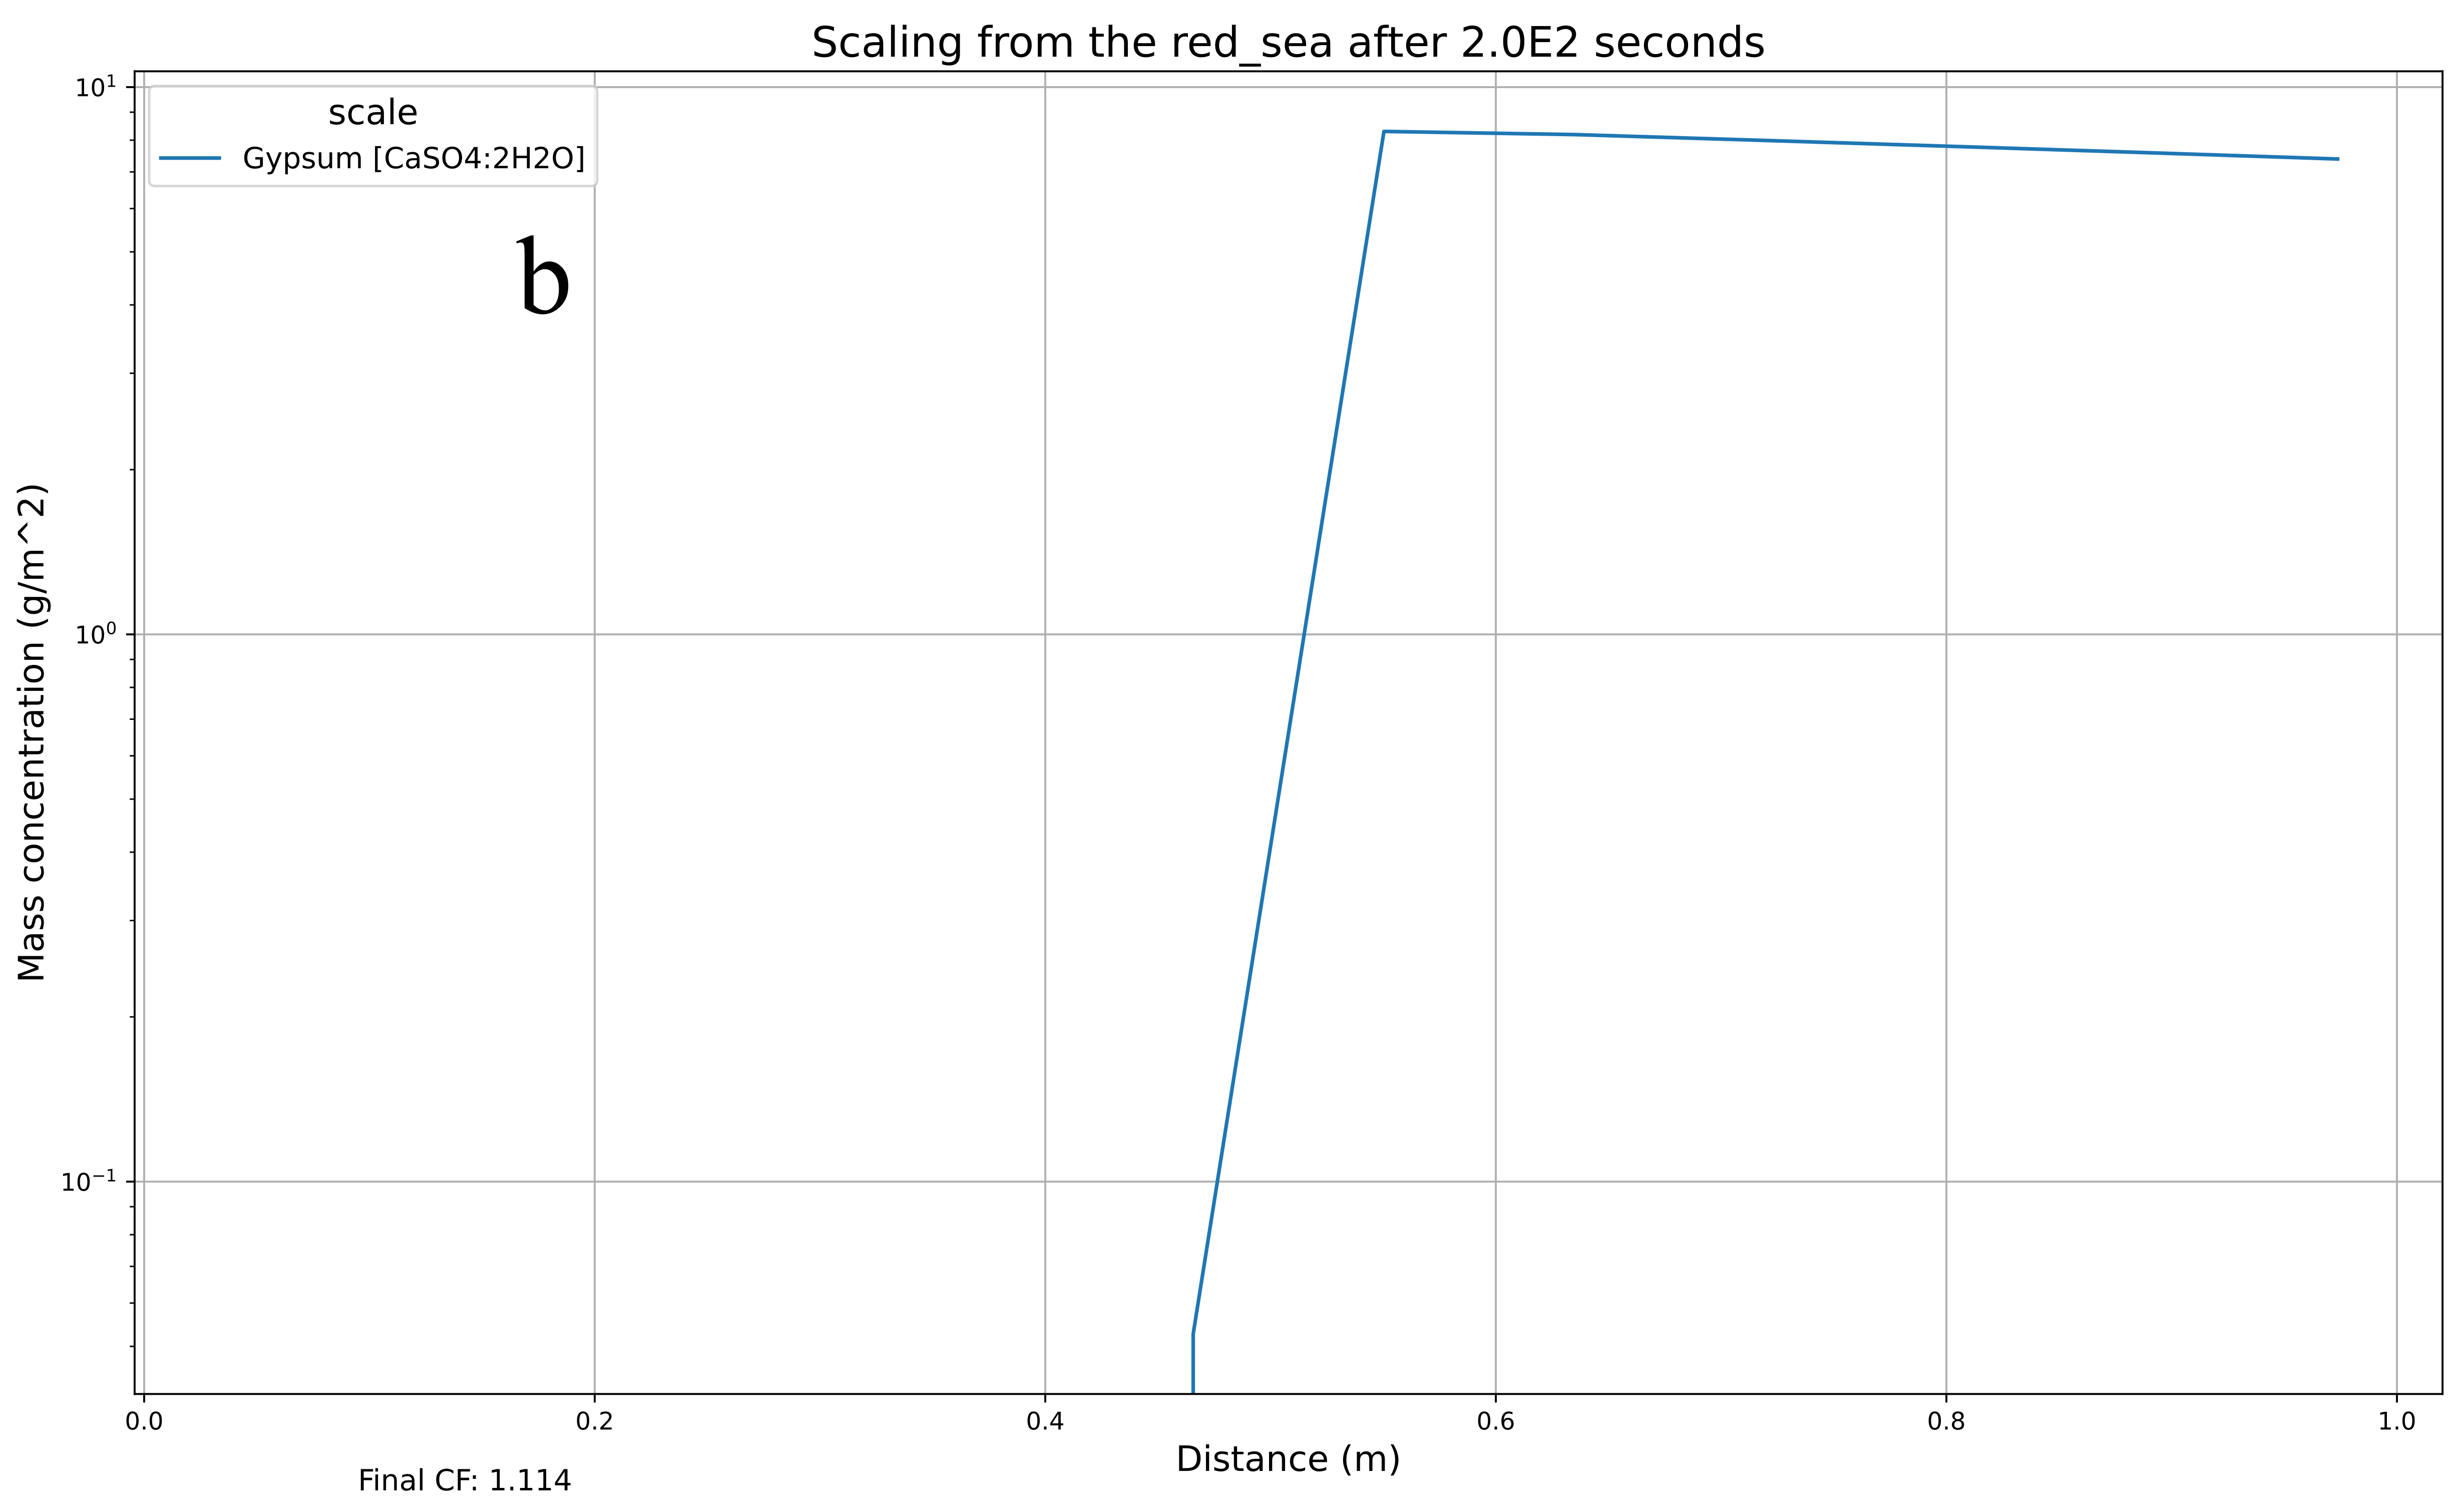
\includegraphics[width=0.9\linewidth]{images/ROSSpy/sensitivity_analyses/permeate_approach/linear_permeate.png} 
    \caption{
        Predicted scaling of the Red Sea at $CF_{effluent}=1.114$ via the a) linear CF and b) linear permeate flux methods. The linear increase in CF of a) slightly homogenizes the distribution of scaling, while the exponential increase in CF of b) skews the distribution of scaling to lesser initially and eventually greater, relative to the linear method of a). These subtle differences in scaling distribution neutralize as the total scaling through both methods are equivalent. 
    }
    \label{permeate_approach}
\end{figure}


\subsubsection{Transport}
The physical transport of feed through the module is simulated in each timestep by 1) migrating the contents of each cell $e$ to the next cell $e+1$; 2) repopulating cell $1$ as new feed solution enters the simulated module; and 3) deleting cell $n$ as brine exits the simulated module. The feed velocity $v_{feed}=\frac{Q_{max~feed}}{A_{feed}}$ is calculated from the maximum feed flowrate $Q_{max~feed}$ ($\frac{m^3}{s}$) and the feed area from \cref{feed_area} of the RO module. Default module parameters in Table S1 are sourced from the DOW FILMTEC BW30-400 RO module, similar to other RO models \cite{Li2012OptimalDesalination}, and supplement user-defined module parameters. The maximum simulation timestep $\Delta t=\frac{l_{cell}}{v_{feed}}$ is calculated according to the Courant Condition \cite{Gnedin2018EnforcingSchemes} ($C_{max}=1 \ge \frac{v_{feed}*t_{max}}{l_{cell}}$) to maintain accurate resolution of the feed flow.

\section{Use cases}
The following sub-sections evince features of our model and its alignment with reported measurements. These studies were conducted through ROSSpy and are available as Python Notebooks in the ROSSpy GitHub repository.

\subsection{CF and Brine formation}
The predicted CF and ionic concentrations of the effluent were verified through comparison with the following three experimental studies, where the reported feed geochemistry and module specifications were parameterized into the model. 

\paragraph{Zaman et al.\cite{Zaman2015DownstreamCompounds}}
This study examines RO brine, from a full-scale water treatment facility in Australia, to understand which minerals are likely to form as scale. The predicted concentrations in Figure \ref{bar_graphs}a were $<6\%-error$ for all but one of the feed ions.

\paragraph{Ahmed et al.\cite{Ahmed2001BrineEmirates}}
This study examines RO brine from 10 small desalination plants in Oman and 8 plants in the United Arab Emirates (UAE) for the purpose of understanding ideal brine disposal methods. We selected the UAE Qidfa I desalination plant from these 18 plants to replicate, since it provided the most comprehensive details. The predicted concentrations in Figure \ref{bar_graphs}b were $<10\%-error$ for all but one of the feed ions. The CF, in the far-right column of Figure \ref{bar_graphs}b, furthermore exhibits a $<1\%-error$, which supports that the reactive transport processes, notably the permeate flux calculations, are accurate.

\paragraph{Hajbi et al.\cite{Hajbi2010ReuseBrine}}
This study  evaluates the recovery of commodity salts from RO brine at a plant in Tunisia. The authors detail specifications of line D -- a polyamide filtration membrane -- in the plant system, in addition to the feed geochemistry, which were all parameterized into our model. The predicted concentrations in Figure \ref{bar_graphs}c were less aligned than the aforementioned two studies, with two ions exceeding $25\%-error$. This is attributed to $40\%$ fewer feed ions being defined by this study, where the incomplete geochemical representation of the feed skews the geochemical calculations of PHREEQC. This is corroborated by the accuracy of the CF prediction in Figure \ref{bar_graphs}c, despite inaccurate concentration predictions, which suggests that the error resides with the geochemical processes and not the reactive transport system. 

\begin{figure}
    \centering
    \begin{tabular}{c|c}
        \multicolumn{2}{c}{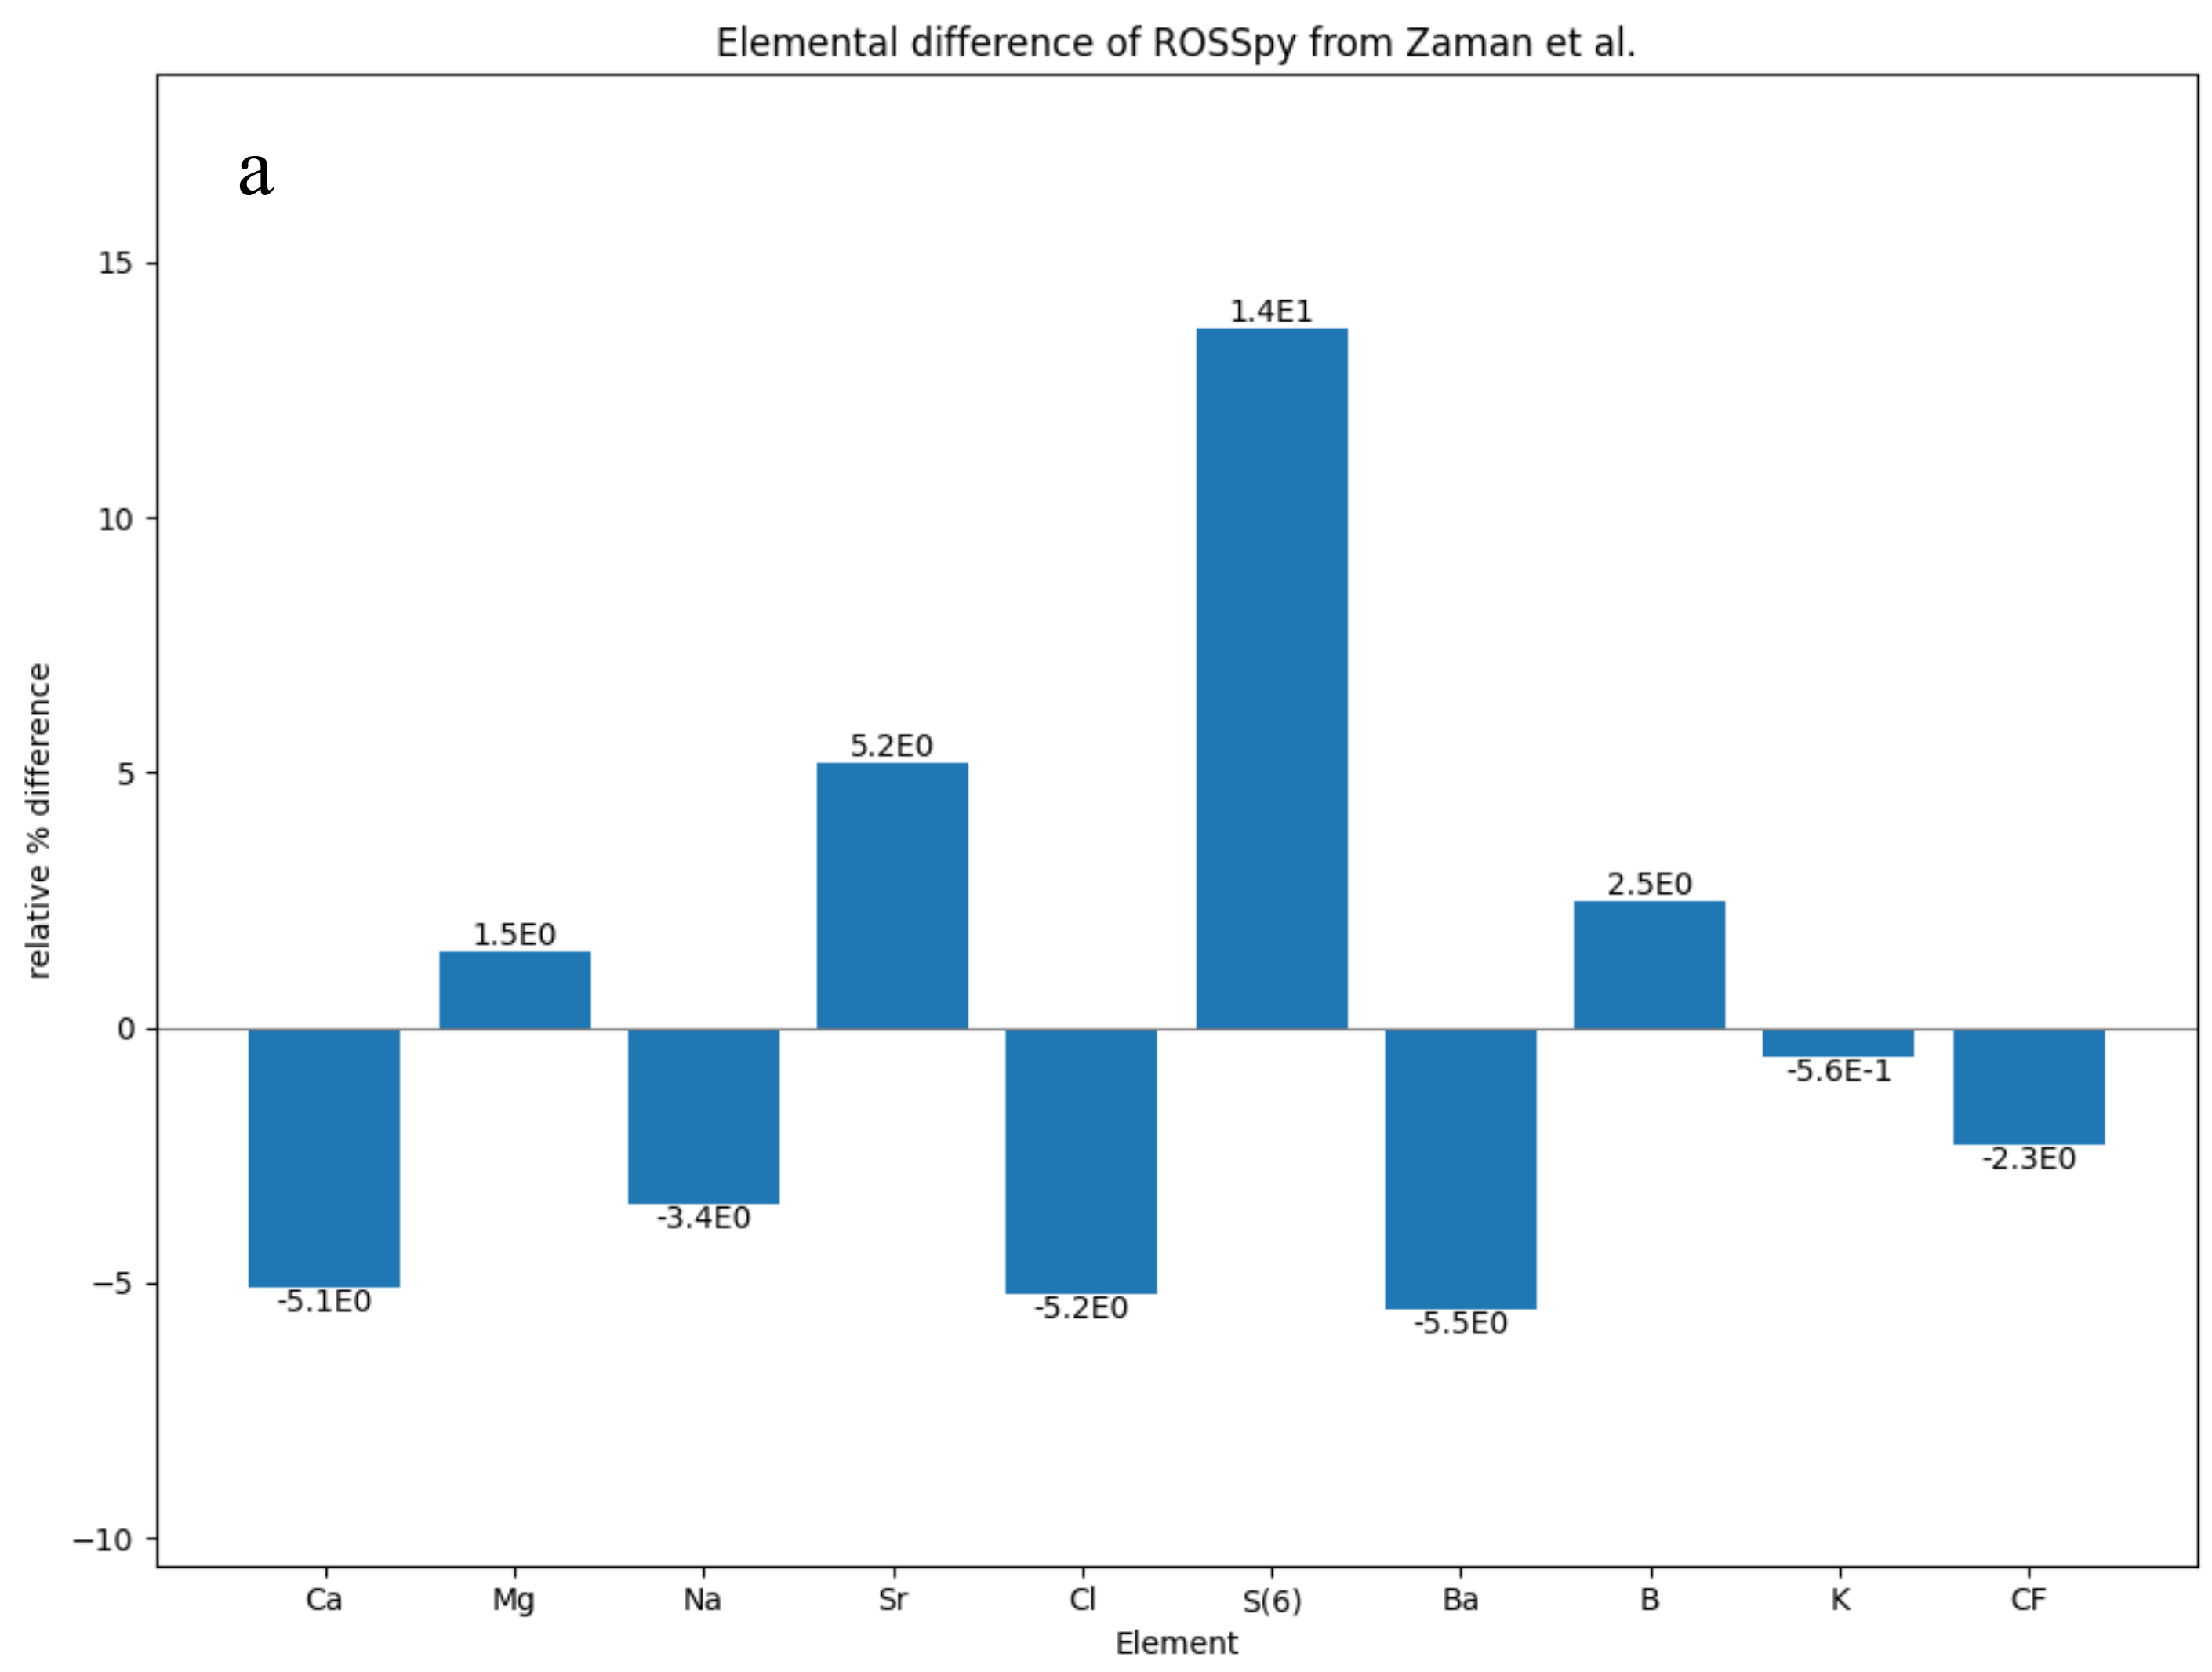
\includegraphics[width=\linewidth]{images/ROSSpy/case_studies/Zaman_comparison.png}} \\ \midrule
        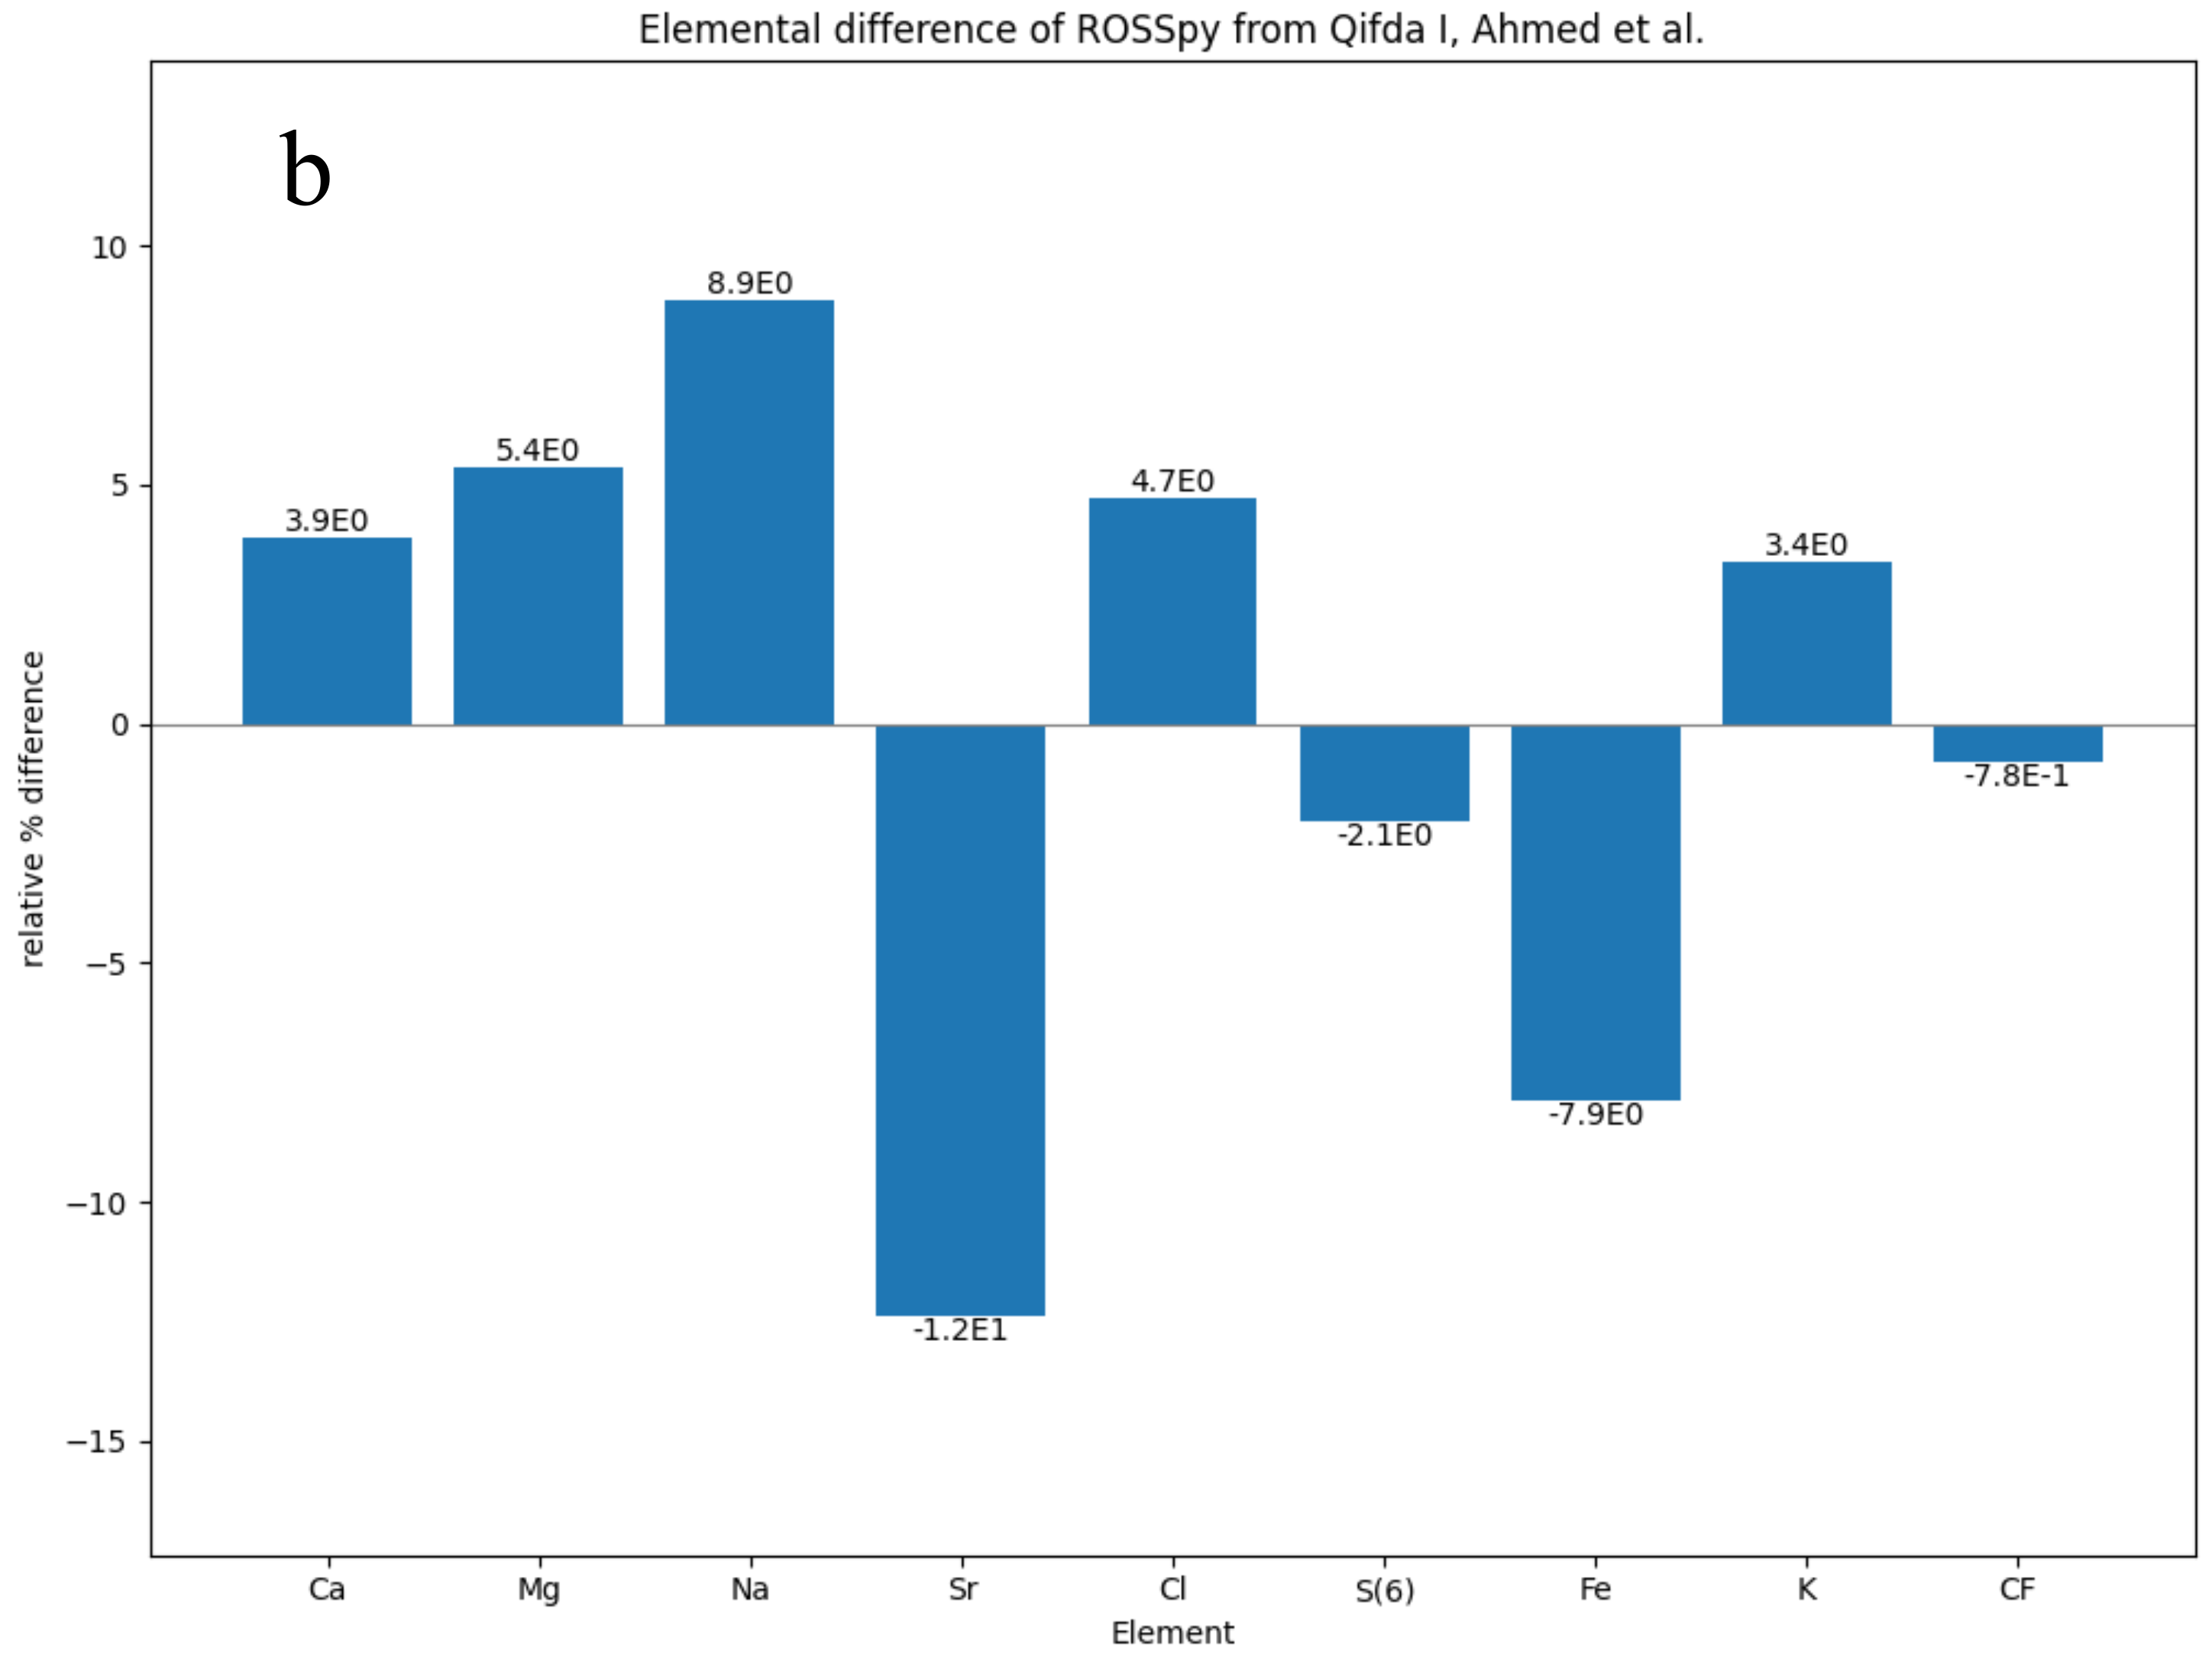
\includegraphics[width=0.49\linewidth]{images/ROSSpy/case_studies/Ahmed_comparison.png} & 
        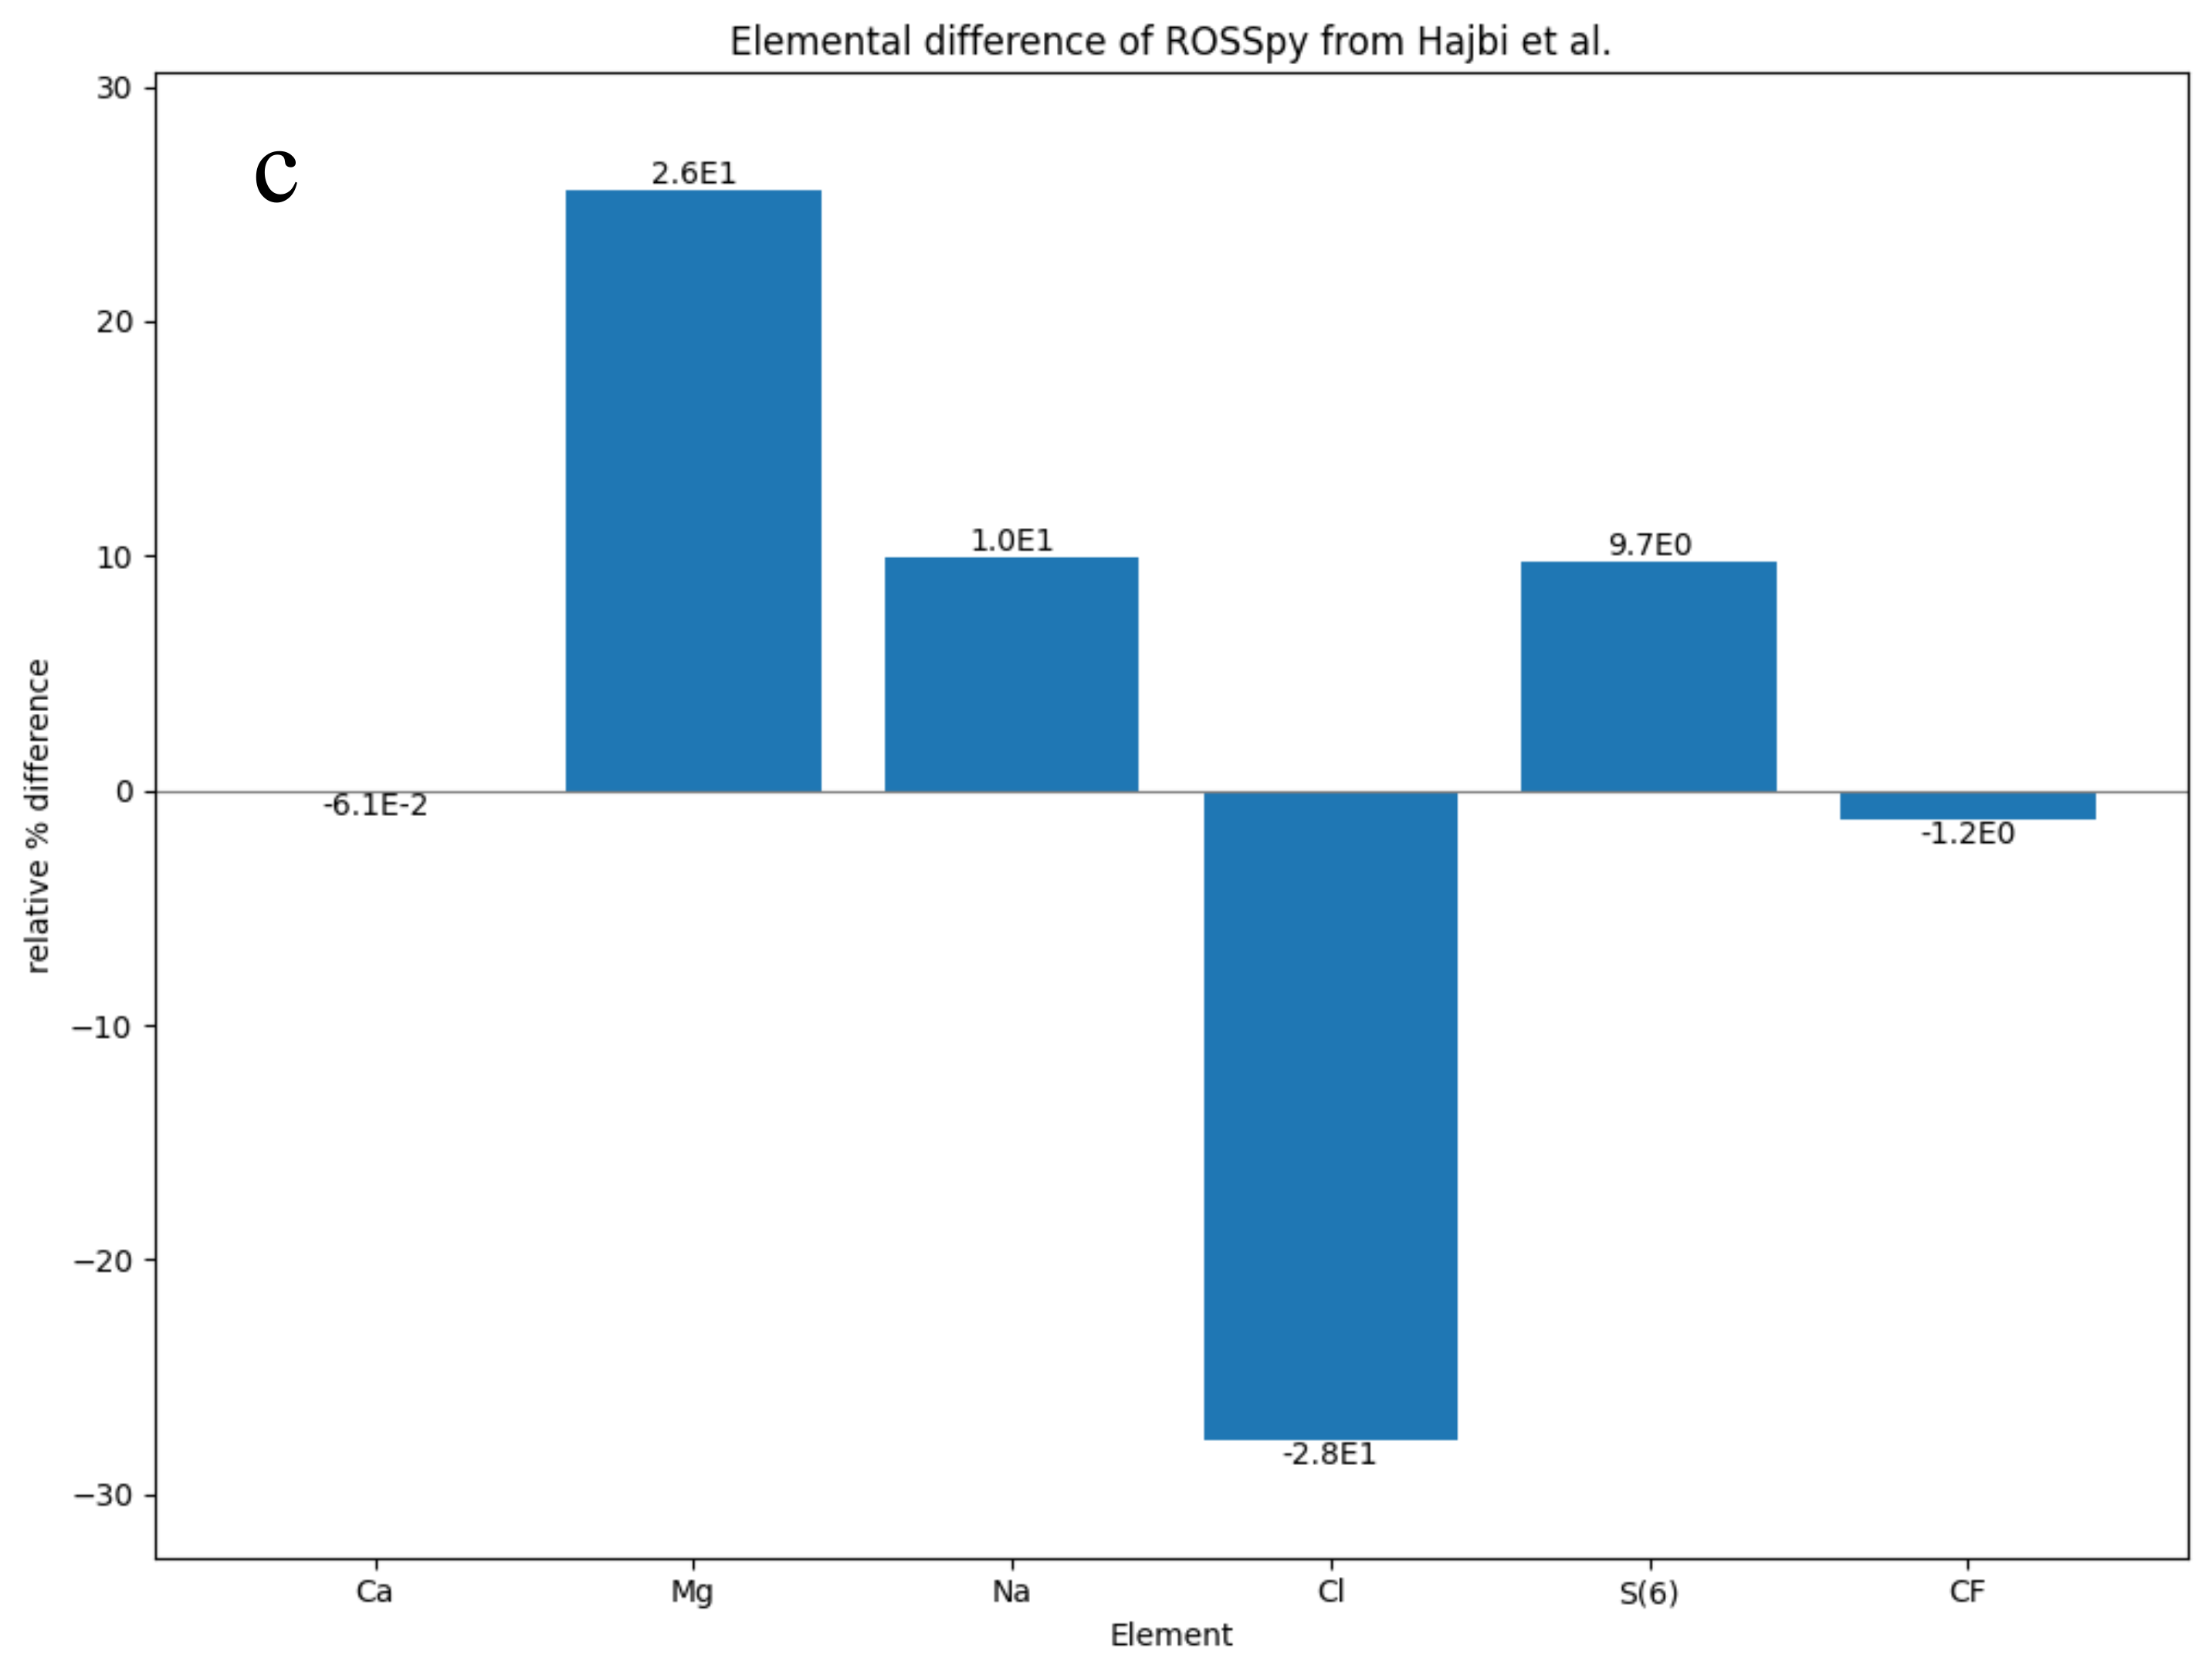
\includegraphics[width=0.49\linewidth]{images/ROSSpy/case_studies/Hajbi_comparison.png} \\ \bottomrule
    \end{tabular}
    \caption{
        The \%-error between predicted and experimental brine concentrations from RO plants. Panels a-c) correspond to comparisons with the Zaman et al. \cite{Zaman2015DownstreamCompounds}, Ahmed et al. \cite{Ahmed2001BrineEmirates}, and Hajbi et al. \cite{Hajbi2010ReuseBrine} studies, respectively, and each possess different y-axis scales to best resolve the bars in each graph. The trend is that prediction accuracy is proportional to the quantity of parameterized ions. 
    }
    \label{bar_graphs}
\end{figure}


\subsection{Scaling}
The scaling predictions were verified qualitatively from experimental literature and quantitatively from theoretical calculations, since experimental literature that quantified scalants with feed geochemistry was not discovered.

\subsubsection{Quantitative}
The quantitative verification consisted of two simple cases of Gypsum precipitation. 1) The first case in Table \ref{gypsum_ice_table} consists of a solution with only $Ca^{2+}$ and $SO_4^{2-}$, where the ionic concentrations decreased by $0.01859$ moles while $0.01961$ moles of Gypsum precipitated. This 5\% discrepancy in mass balance is attributed to the printed PHREEQC values in this calculation neglecting diffusion within the feed solution, yet diffusion is considered in the final output of PHREEQC. 2) The second case in Table S1 evaluates Gypsum precipitation from desalinating the solution from the first case with that from the Red Sea, which only precipitates Gypsum in our model. The simple solution precipitated $0.181$ moles of Gypsum, while the Red Sea precipitated $0.194$ moles. This $+7\%$-error is attributed to ionic interactions within the Red Sea feed that are not present by the simple solution of only $Ca^{2+}$ and $SO_4^{2-}$. These subtle $[5,7]\%$ deviations, even without considering the coarse assumptions in these simple examples, are relatively minor in the context of other sources of error, such as feed measurements, and still elicit quantitative consistency in scaling predictions.

\begin{table}
    \centering
    \begin{tabular}{c|ccccc}
      \toprule
       & $Ca^{2+}$ & $+$ & $SO_4^{2-}$ & $\leftrightharpoons$ & $CaSO_4$ \\
      \midrule
      I & $0.3545$ && $1.816$ && $0$ \\
      C & $-0.01859$ && $-0.01859$ && $+0.01961$ \\
      F & $0.3360$ && $1.797$ && $0.01961$ \\
      \bottomrule
    \end{tabular}
    \caption{
        Gypsum precipitation according to the ICE (Initial, Change, Equilibrium) framework, except that "Equilibrium" (E) is replaced with "Final" (F) since the system does not completely reach equilibrium within the RO module. The $5\%-error$ in row C, between the changes in ionic and Gypsum moles, suggests a subtle discrepancy in mass balance of PHREEQC; however, this is attributed to PHREEQC printing values before diffusion is incorporated in the calculations, per David Parkhurst. 
      }
    \label{gypsum_ice_table}
\end{table}

\subsubsection{Qualitative}
The scaling predictions were qualitatively verified through three experimental studies. 

\paragraph{Karabelas et al., 2020 \cite{Karabelas2020ScalingTools}}
This study inspired features of ROSSpy by reviewing the state-of-the-art, and future directions, for predictive scaling software. The study also, importantly, describes in its Supporting Information scalants that were observed after desalination with defined conditions. Scaling predictions from these conditions in Figure \ref{qualitative_scaling}a, over a few PHREEQC databases, match the reported scalants ("Calcite but not Gypsum" and a "few other salts, such as Barite and Dolomite, could also deposit at downstream...") in numerous aspects: 1) Calcite was the primary scalant; 2) Gypsum was not observed; 3) a few other salts precipitated, including Dolomite and Barite, depending upon the PHREEQC database; and 4) these other salts precipitated primarily in the downstream portion of the module.  

\paragraph{Karabelas et al., 2014 \cite{Karabelas2014IncipientChannels}}
This study elucidates the mechanisms of incipient scaling from RO desalination -- with Gypsum as the archetypal scalant \cite{Lyster2009CoupledModule}. The ID 28SC trial, which was the most thoroughly described trial, was simulated and Gypsum was the only predicted scalant in Figure \ref{qualitative_scaling}b, just as the reported scalant.  

\paragraph{Lee et al., 2009 \cite{Lee2009MembraneWastewater}}
This study evaluates the use of a membrane bioreactor -- a hollow-fiber membrane module design that is mechanistically similar to RO and thus can be represented by our model -- to treat wastewater. The wastewater filtration system was simulated, and the only predicted scalant was Calcite in Figure \ref{qualitative_scaling}c, just as the reported scalant.

\begin{figure}
    \begin{tabular}{c|c}
        \multicolumn{2}{c}{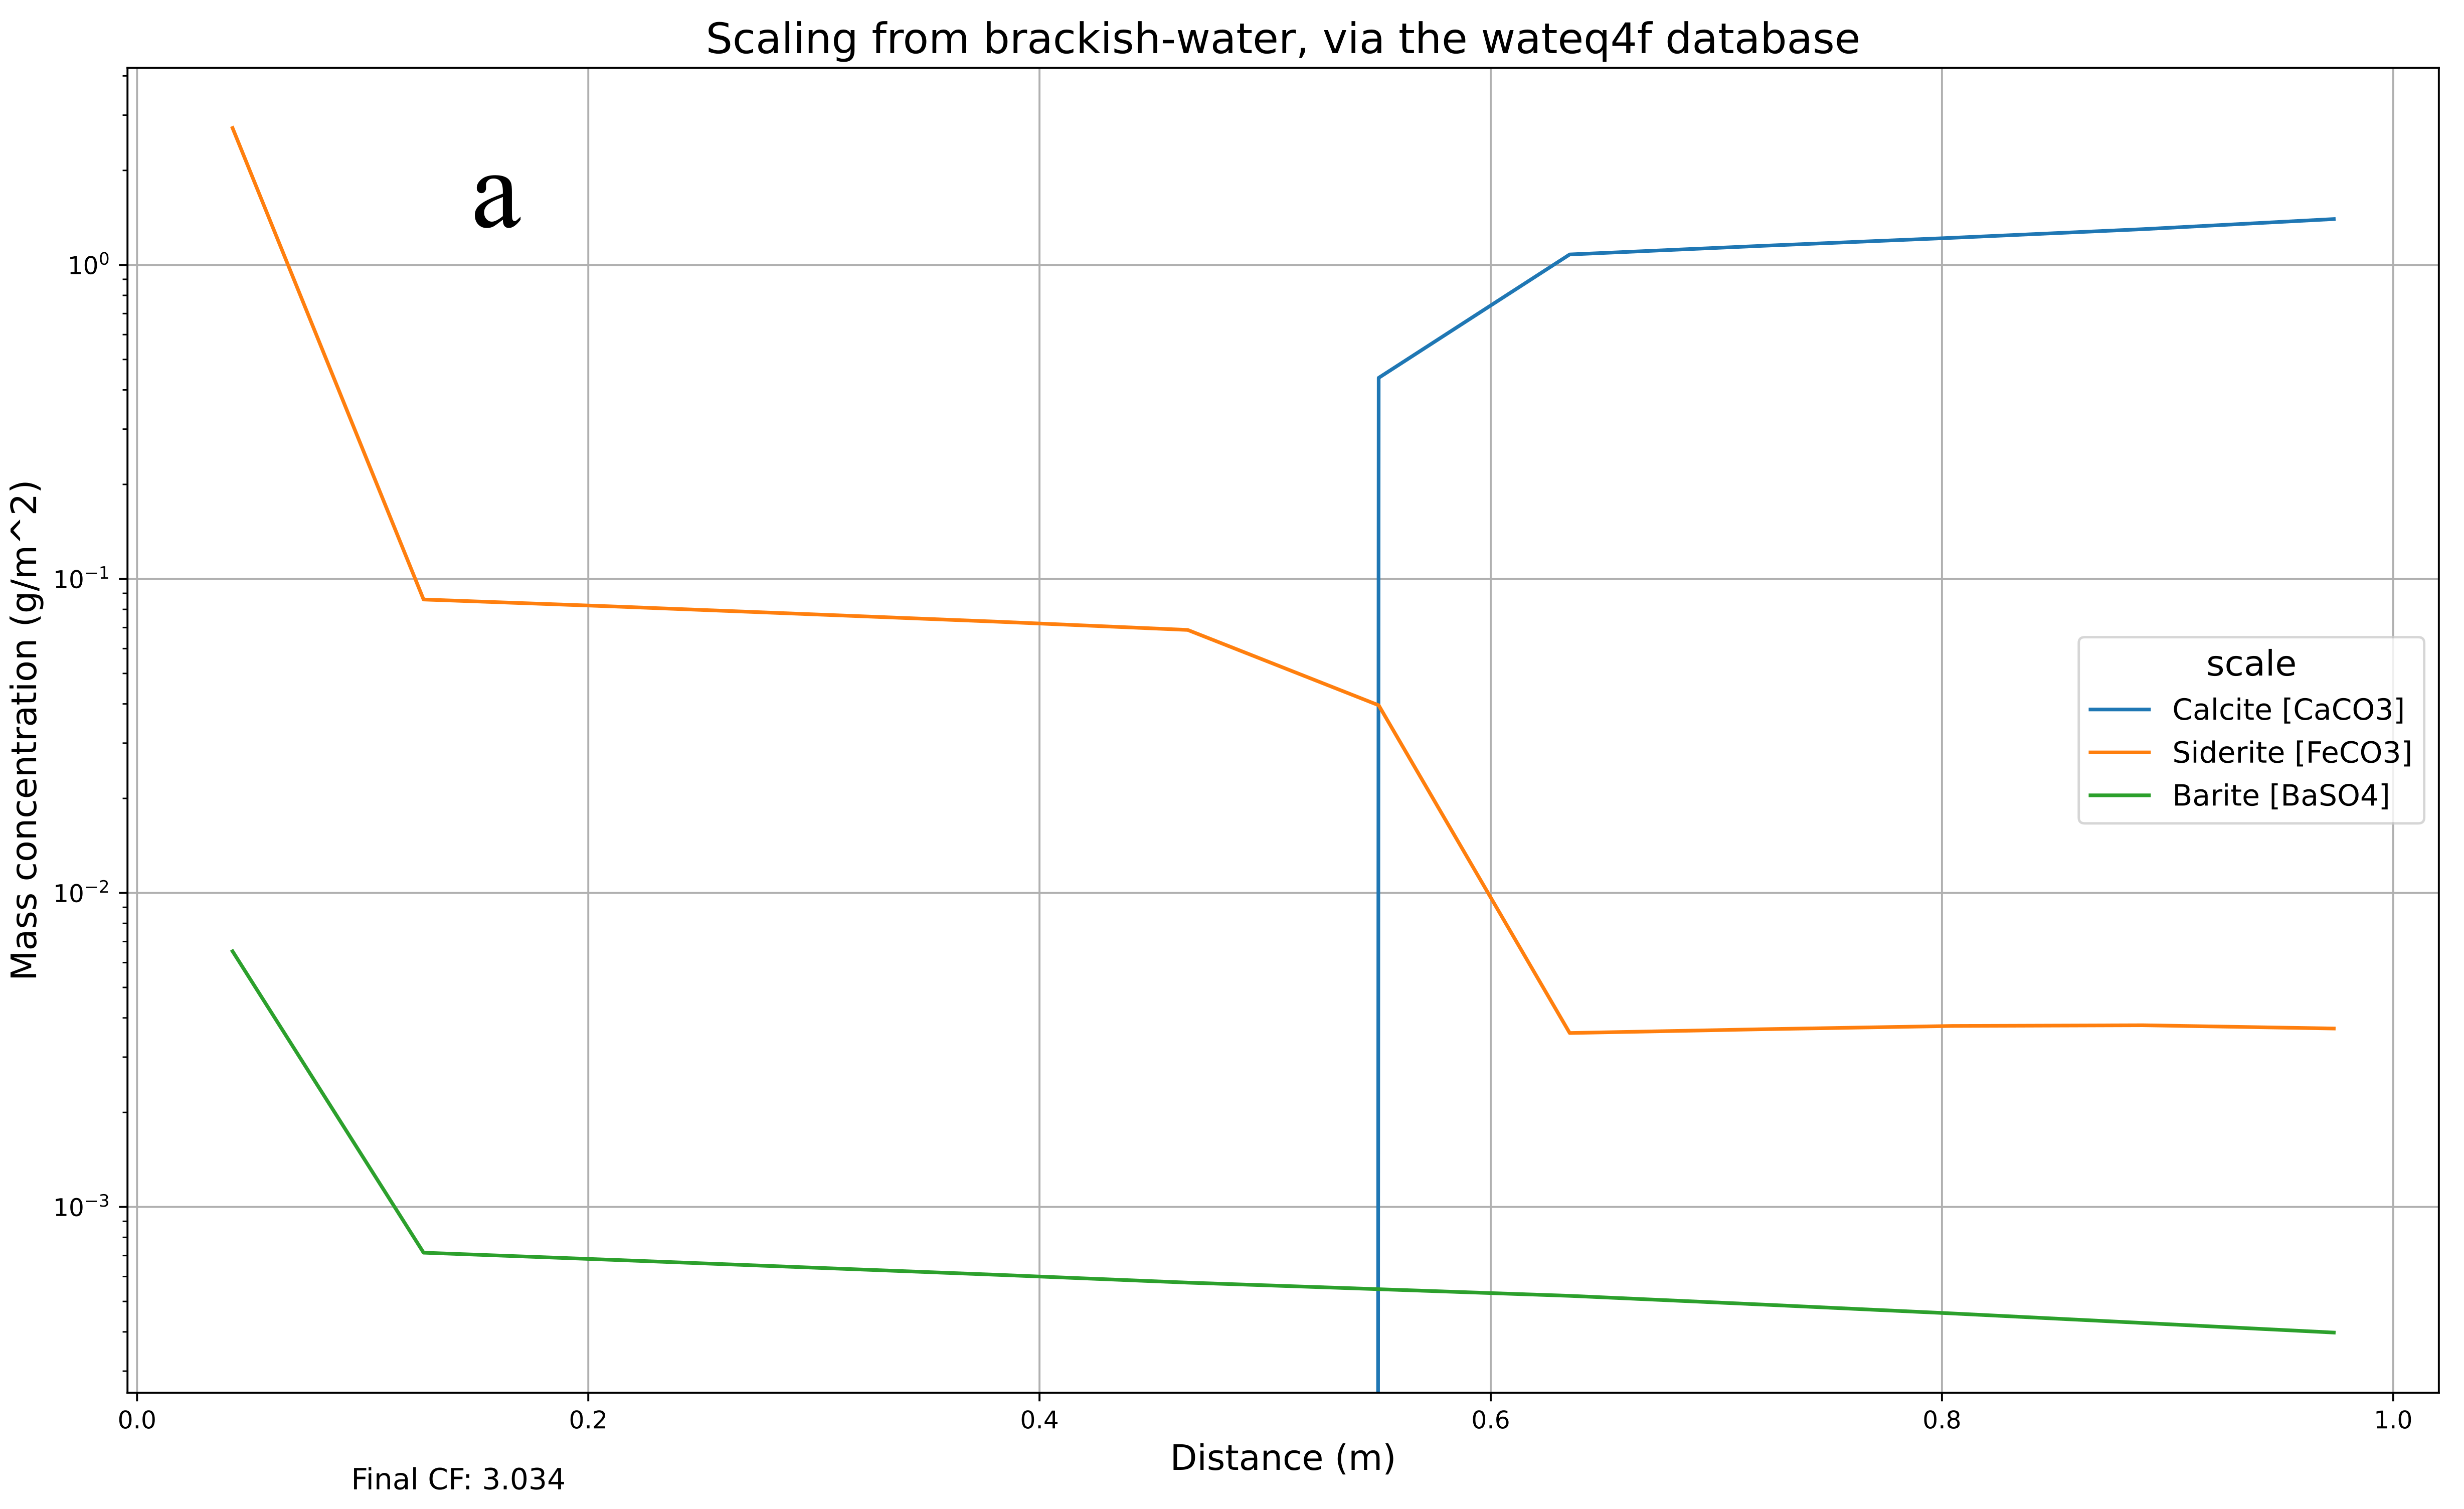
\includegraphics[width=\linewidth]{images/ROSSpy/case_studies/Karabelas_2020_wateq4f.png}} \\
        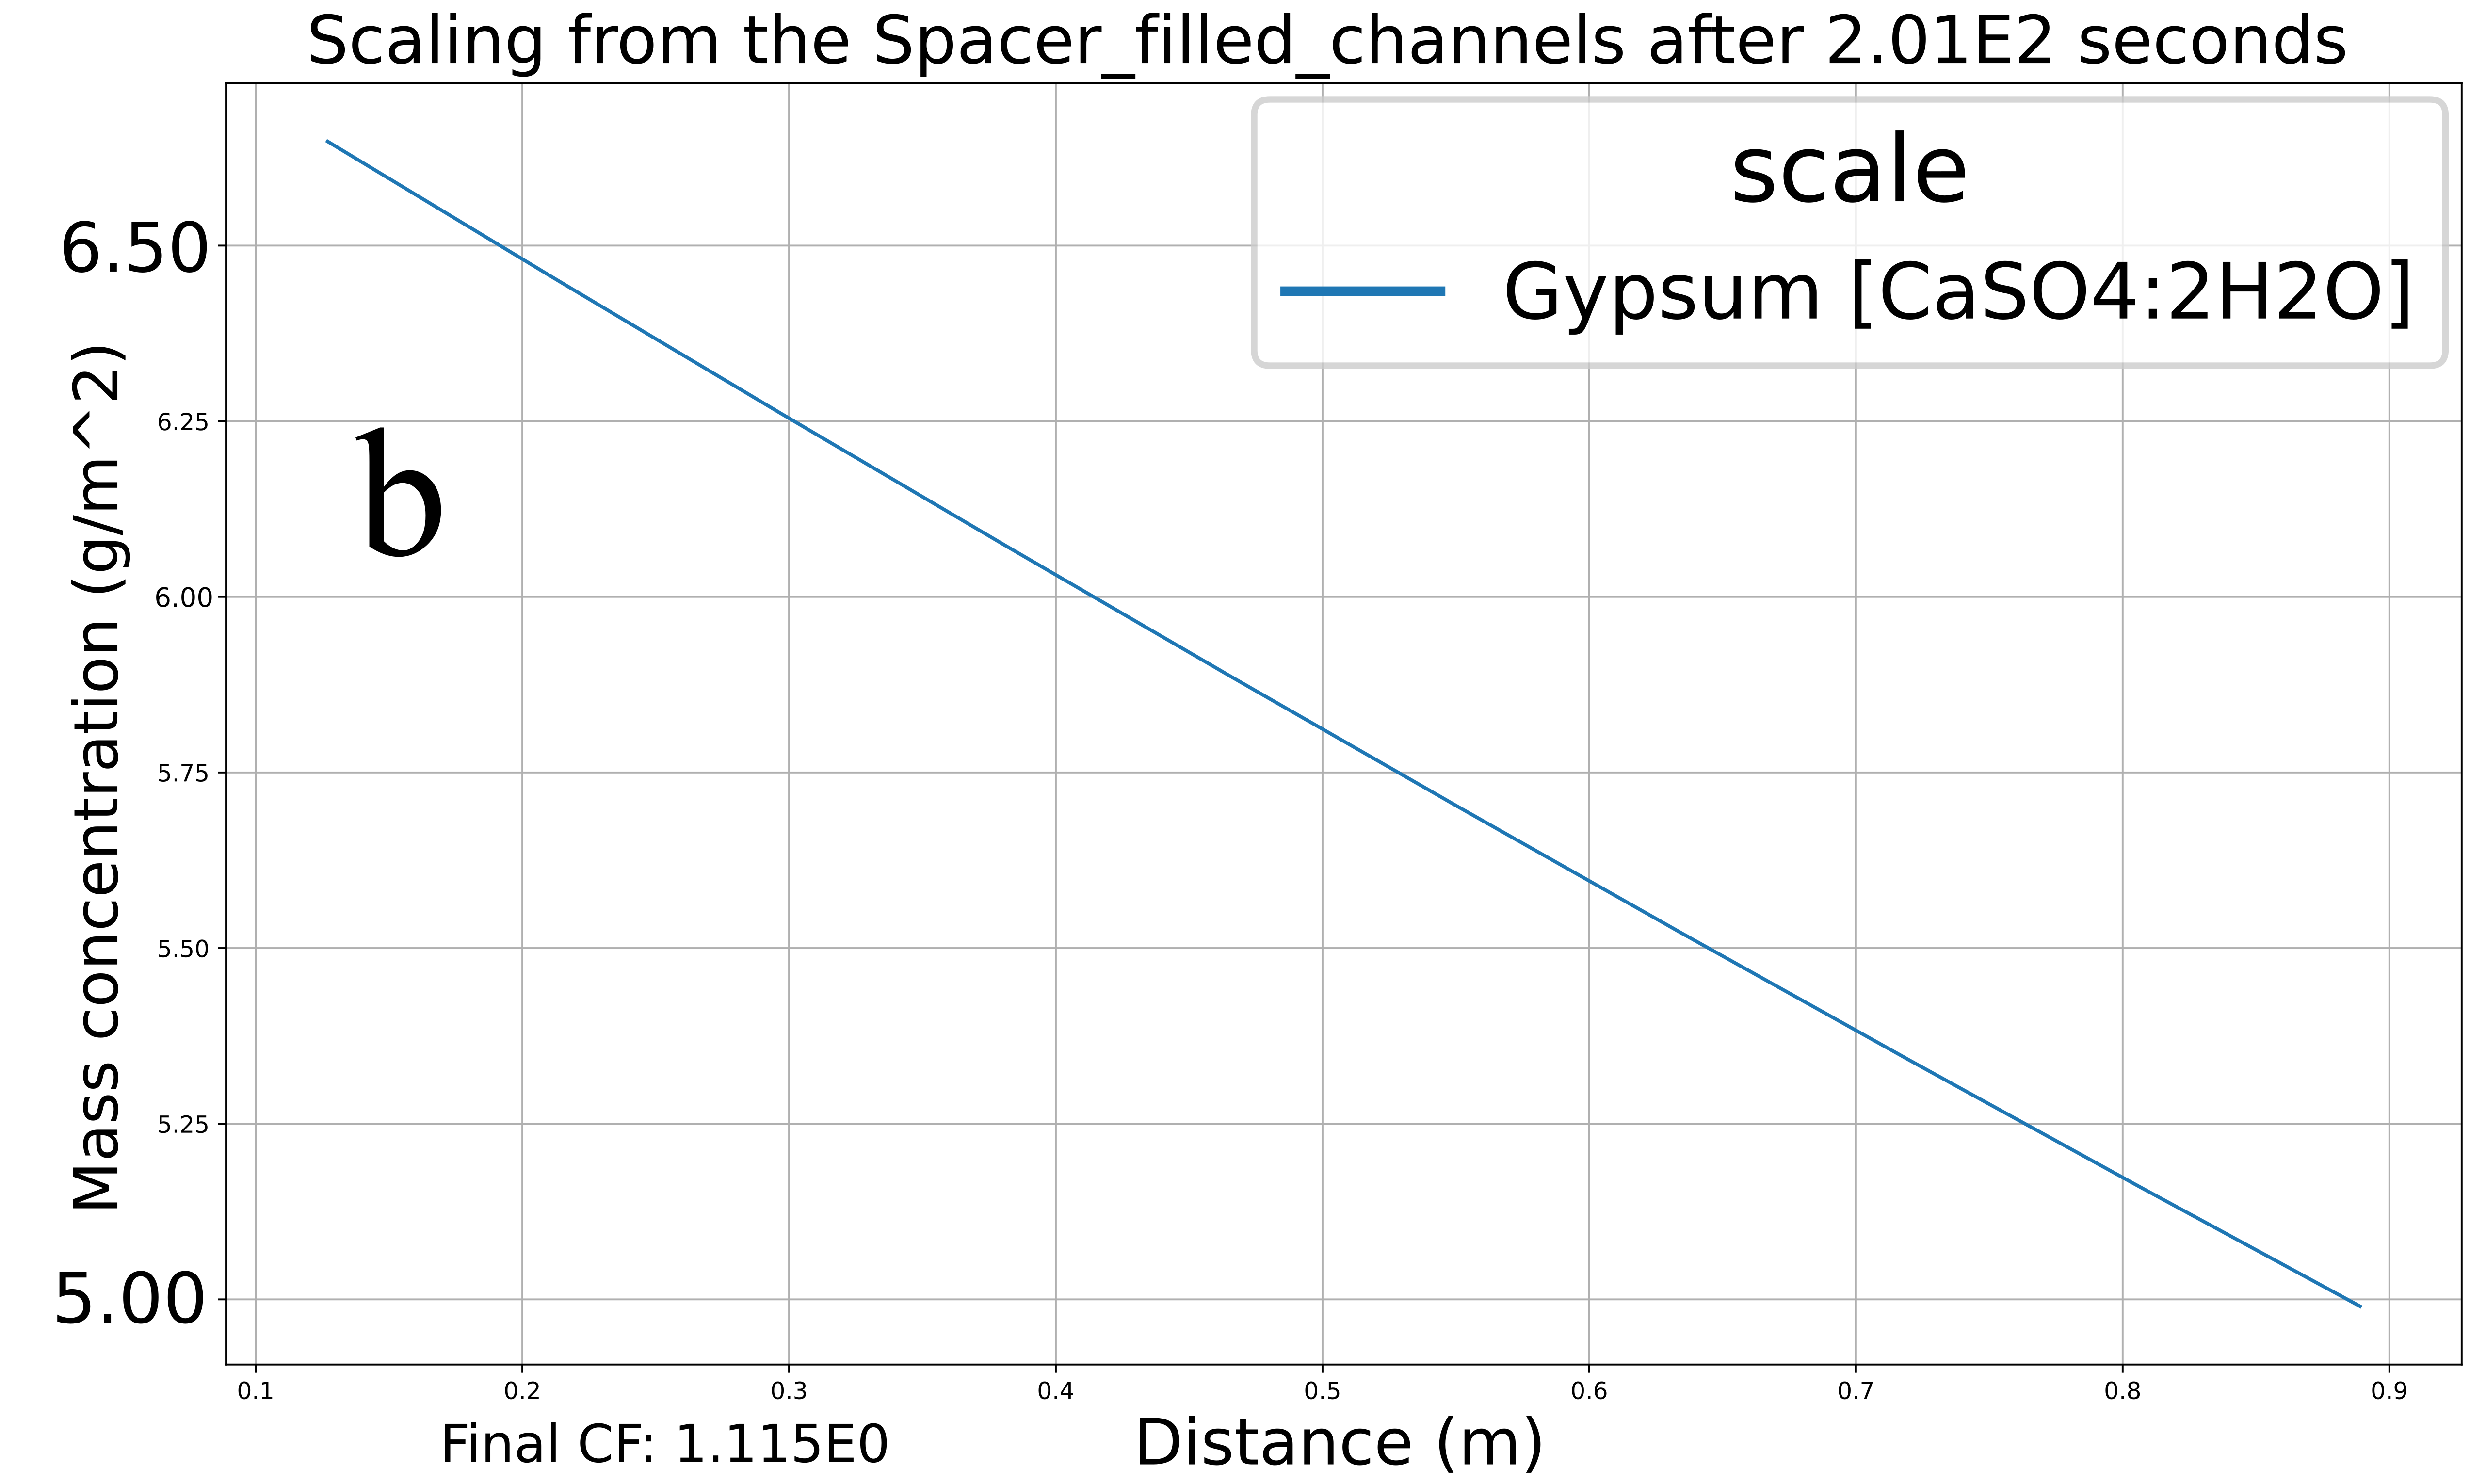
\includegraphics[width=0.49\linewidth]{images/ROSSpy/case_studies/Karabelas_2014_pitzer.png} 
        & 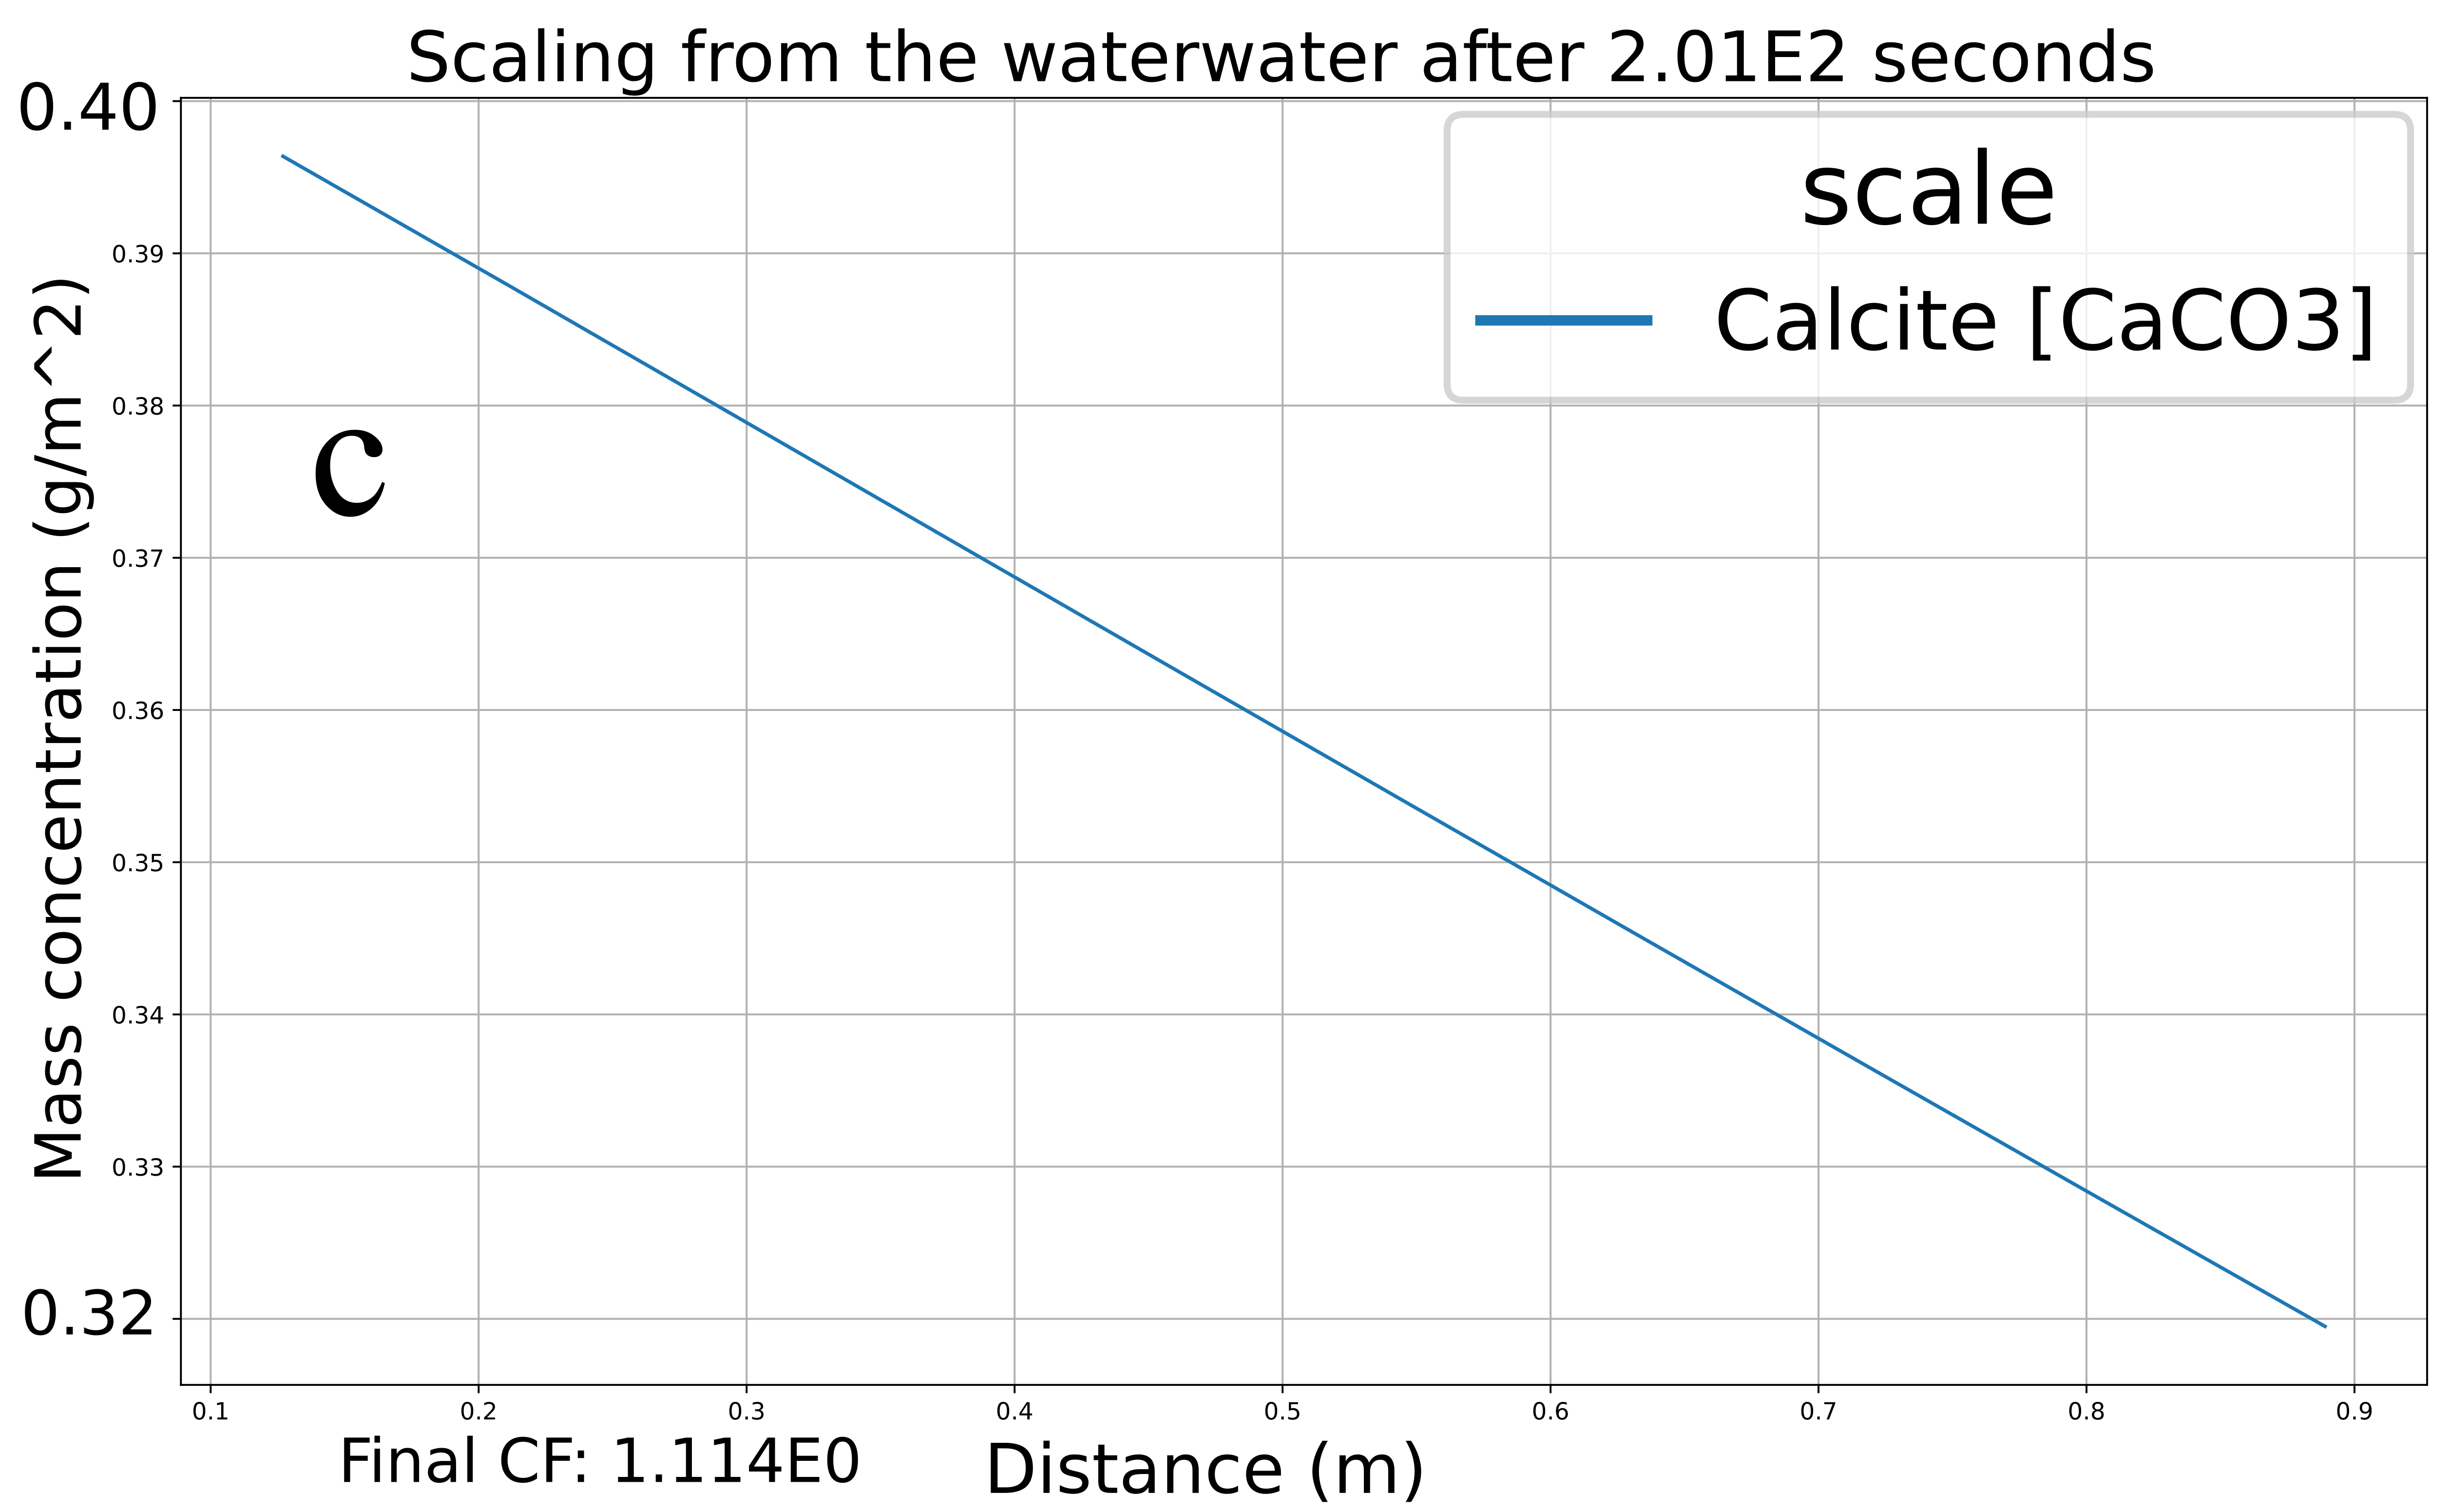
\includegraphics[width=0.49\linewidth]{images/ROSSpy/case_studies/Lee_pitzer.png} \\
    \end{tabular}
    \caption{
        The qualitative validation of scaling for a) multiple minerals from the Karabelas et al., 2020 study; b) Gypsum in the Karabelas et al., 2014 study; and c) Calcite in the Lee et al. study. 
    }
    \label{qualitative_scaling}
\end{figure}


\section{Sensitivity analyses}
A few sensitivity analyses were conducted with major variables in the following subsections. Additional sensitivity analyses of lesser parameters are presented in the Supporting Information.

\subsection{Database section}
The PHREEQC databases crucially 1) determines the set of minerals that can be simulated; 2) contains all of the kinetic, thermodynamic, and stoichiometric information of each mineral; and 3) employs a chemical activity model: e.g. Pitzer, Debye-H\"uckel, and Davies in Section 7 of the Supporting Information. The Pitzer model \cite{Pitzer1973ThermodynamicsEquations,Pitzer1974ThermodynamicsElectrolytes}, which is implemented in the pitzer PHREEQC database, is touted as being supremely accurate in the concentration range of desalination \cite{VandeLisdonk2001PredictionSystems,Sheikholeslami2004AssessmentUnits,Mohammad2007PredictionMembranes}; however, the narrow breadth of accepted ions and minerals may justify using other databases, such as wateq4, for complex or uncommon feed sources. Each of the 13 databases were simulated in desalinating the Red Sea, where the $Amm$, $Core10$, $LLNL$, and $Minteq.v4$ databases failed to numerically converge while the scaling predictions from the other $\frac{9}{13}$ databases are summarized in Figure \ref{database_selection}. The database selection evidently alters scaling predictions; thus, the database must be carefully selected for a given system after reviewing the PHREEQC User Manual or inquirying to the PHREEQC user forum \url{PHREEQCusers.org}.

\begin{figure}
    \centering
    \begin{tabular}{c|c}
        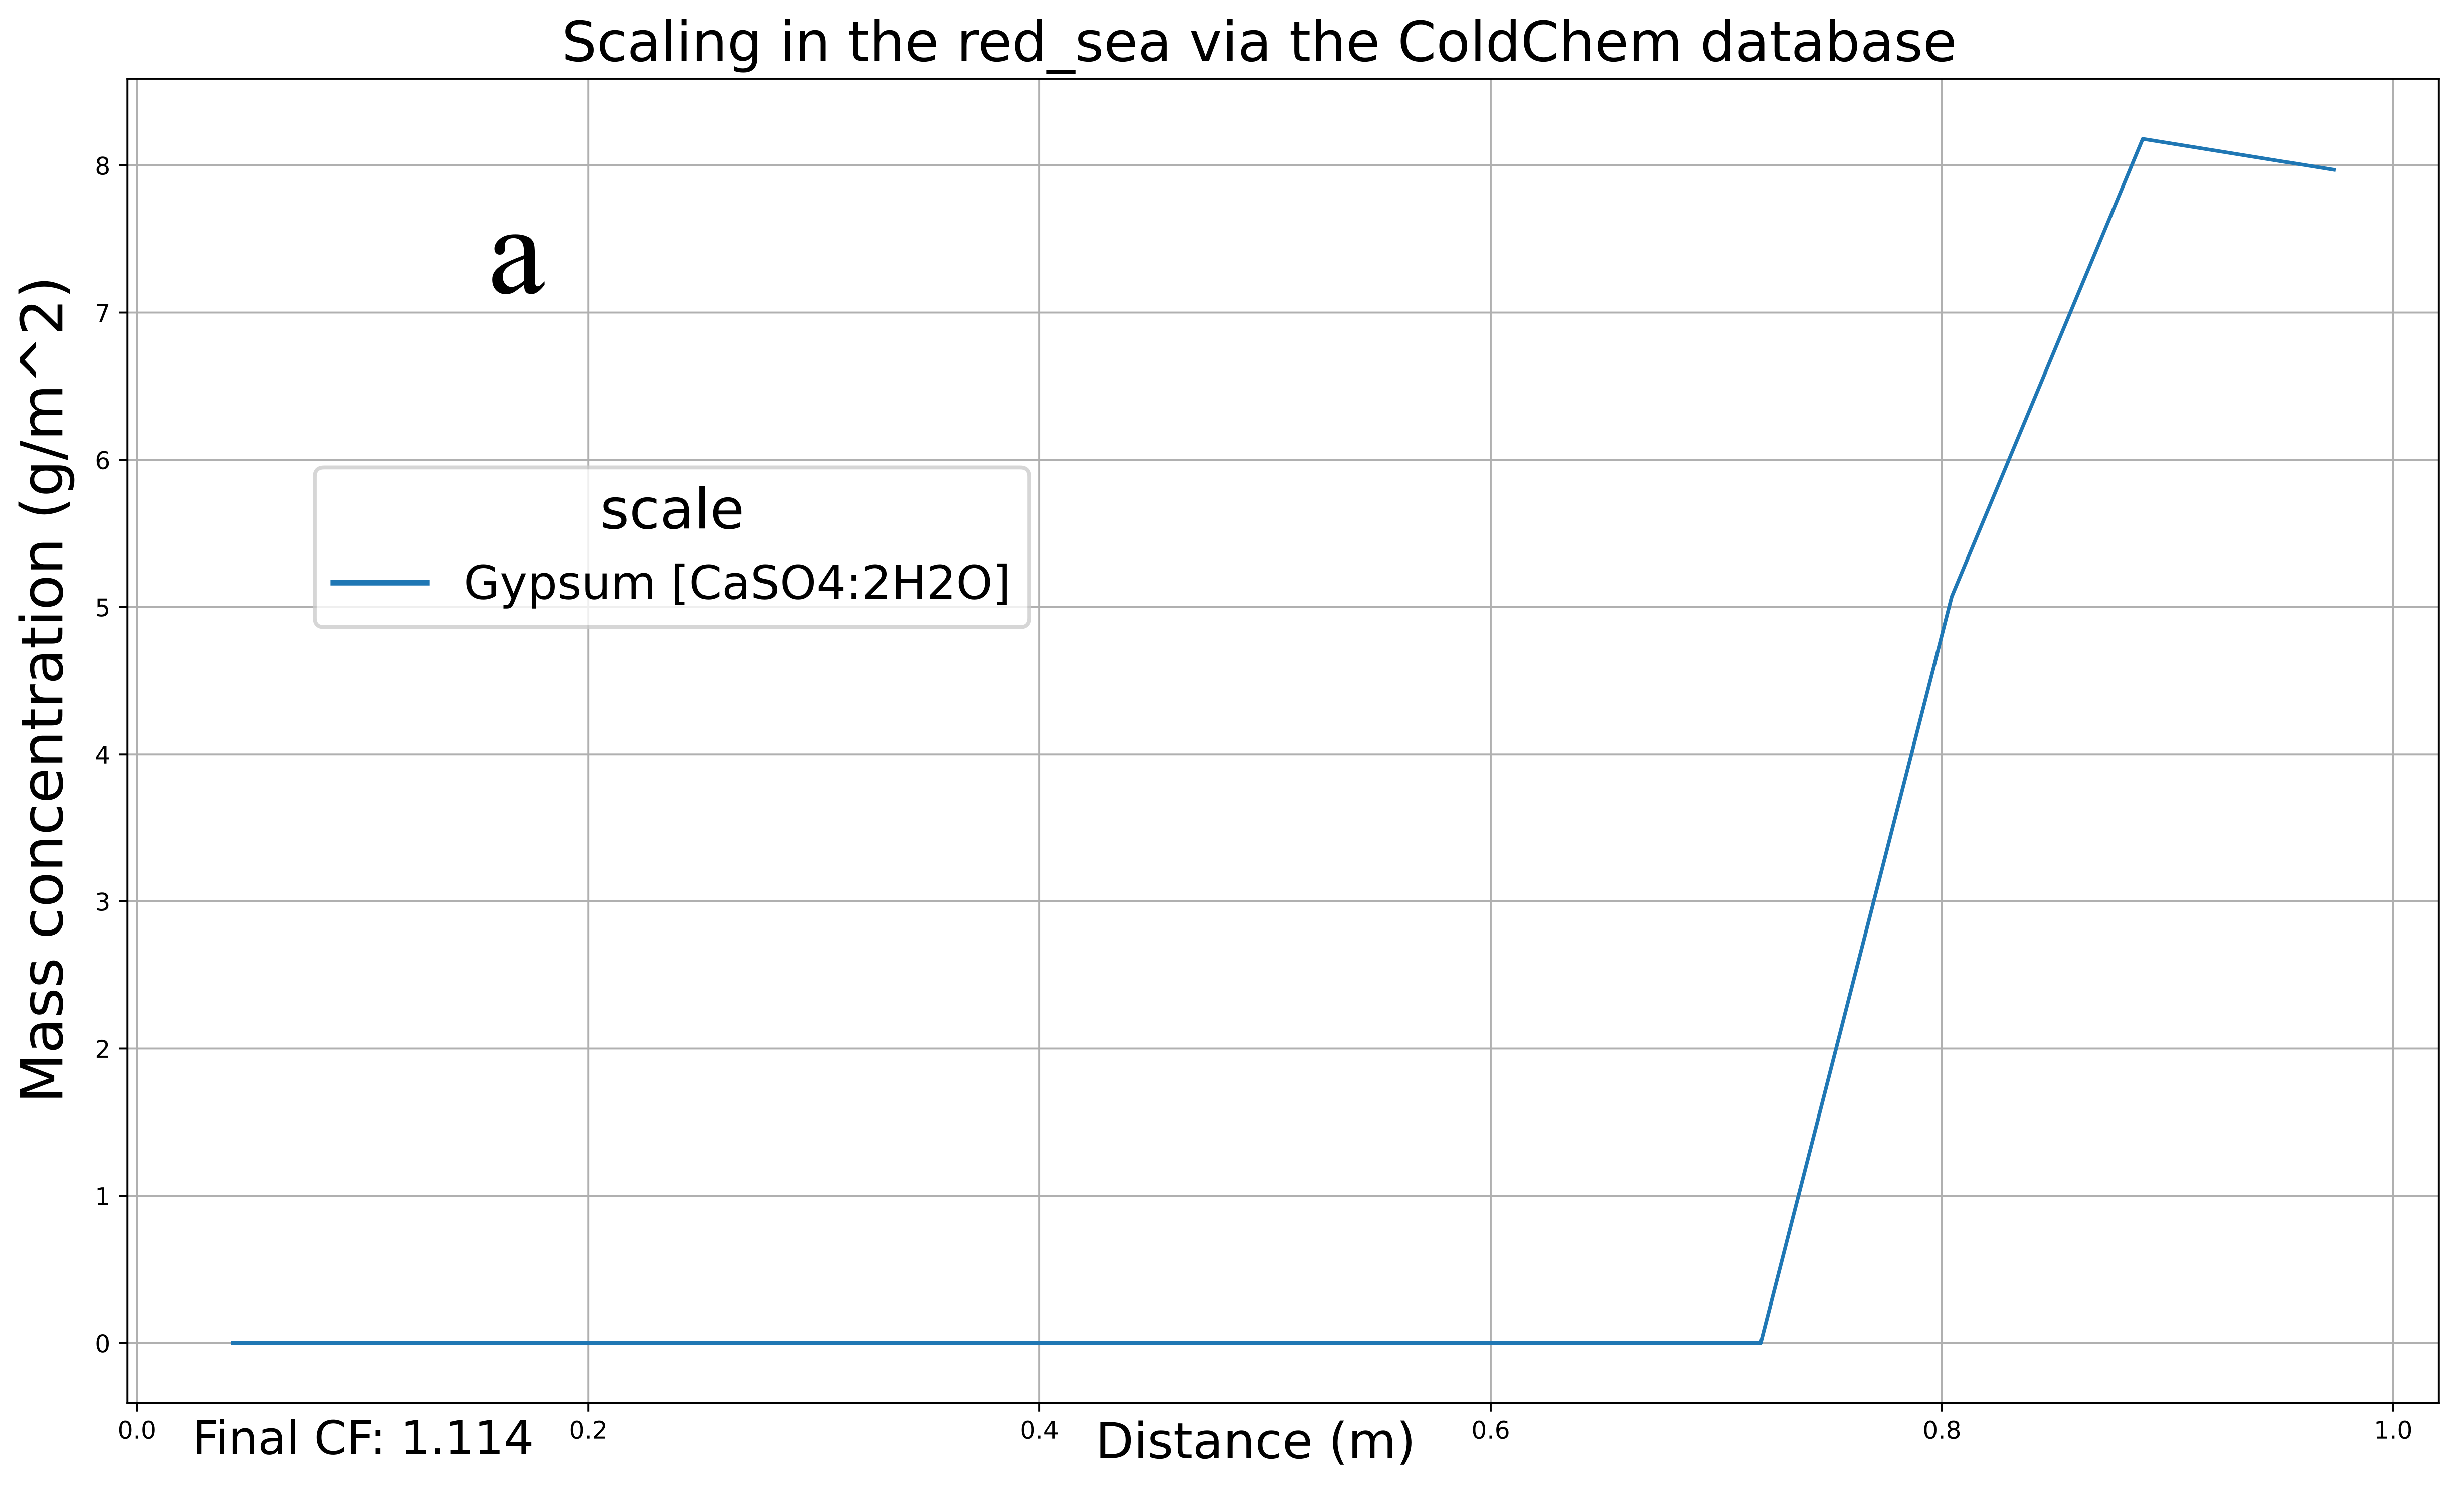
\includegraphics[width=0.49\textwidth]{images/ROSSpy/sensitivity_analyses/databases/ColdChem.png} 
        & 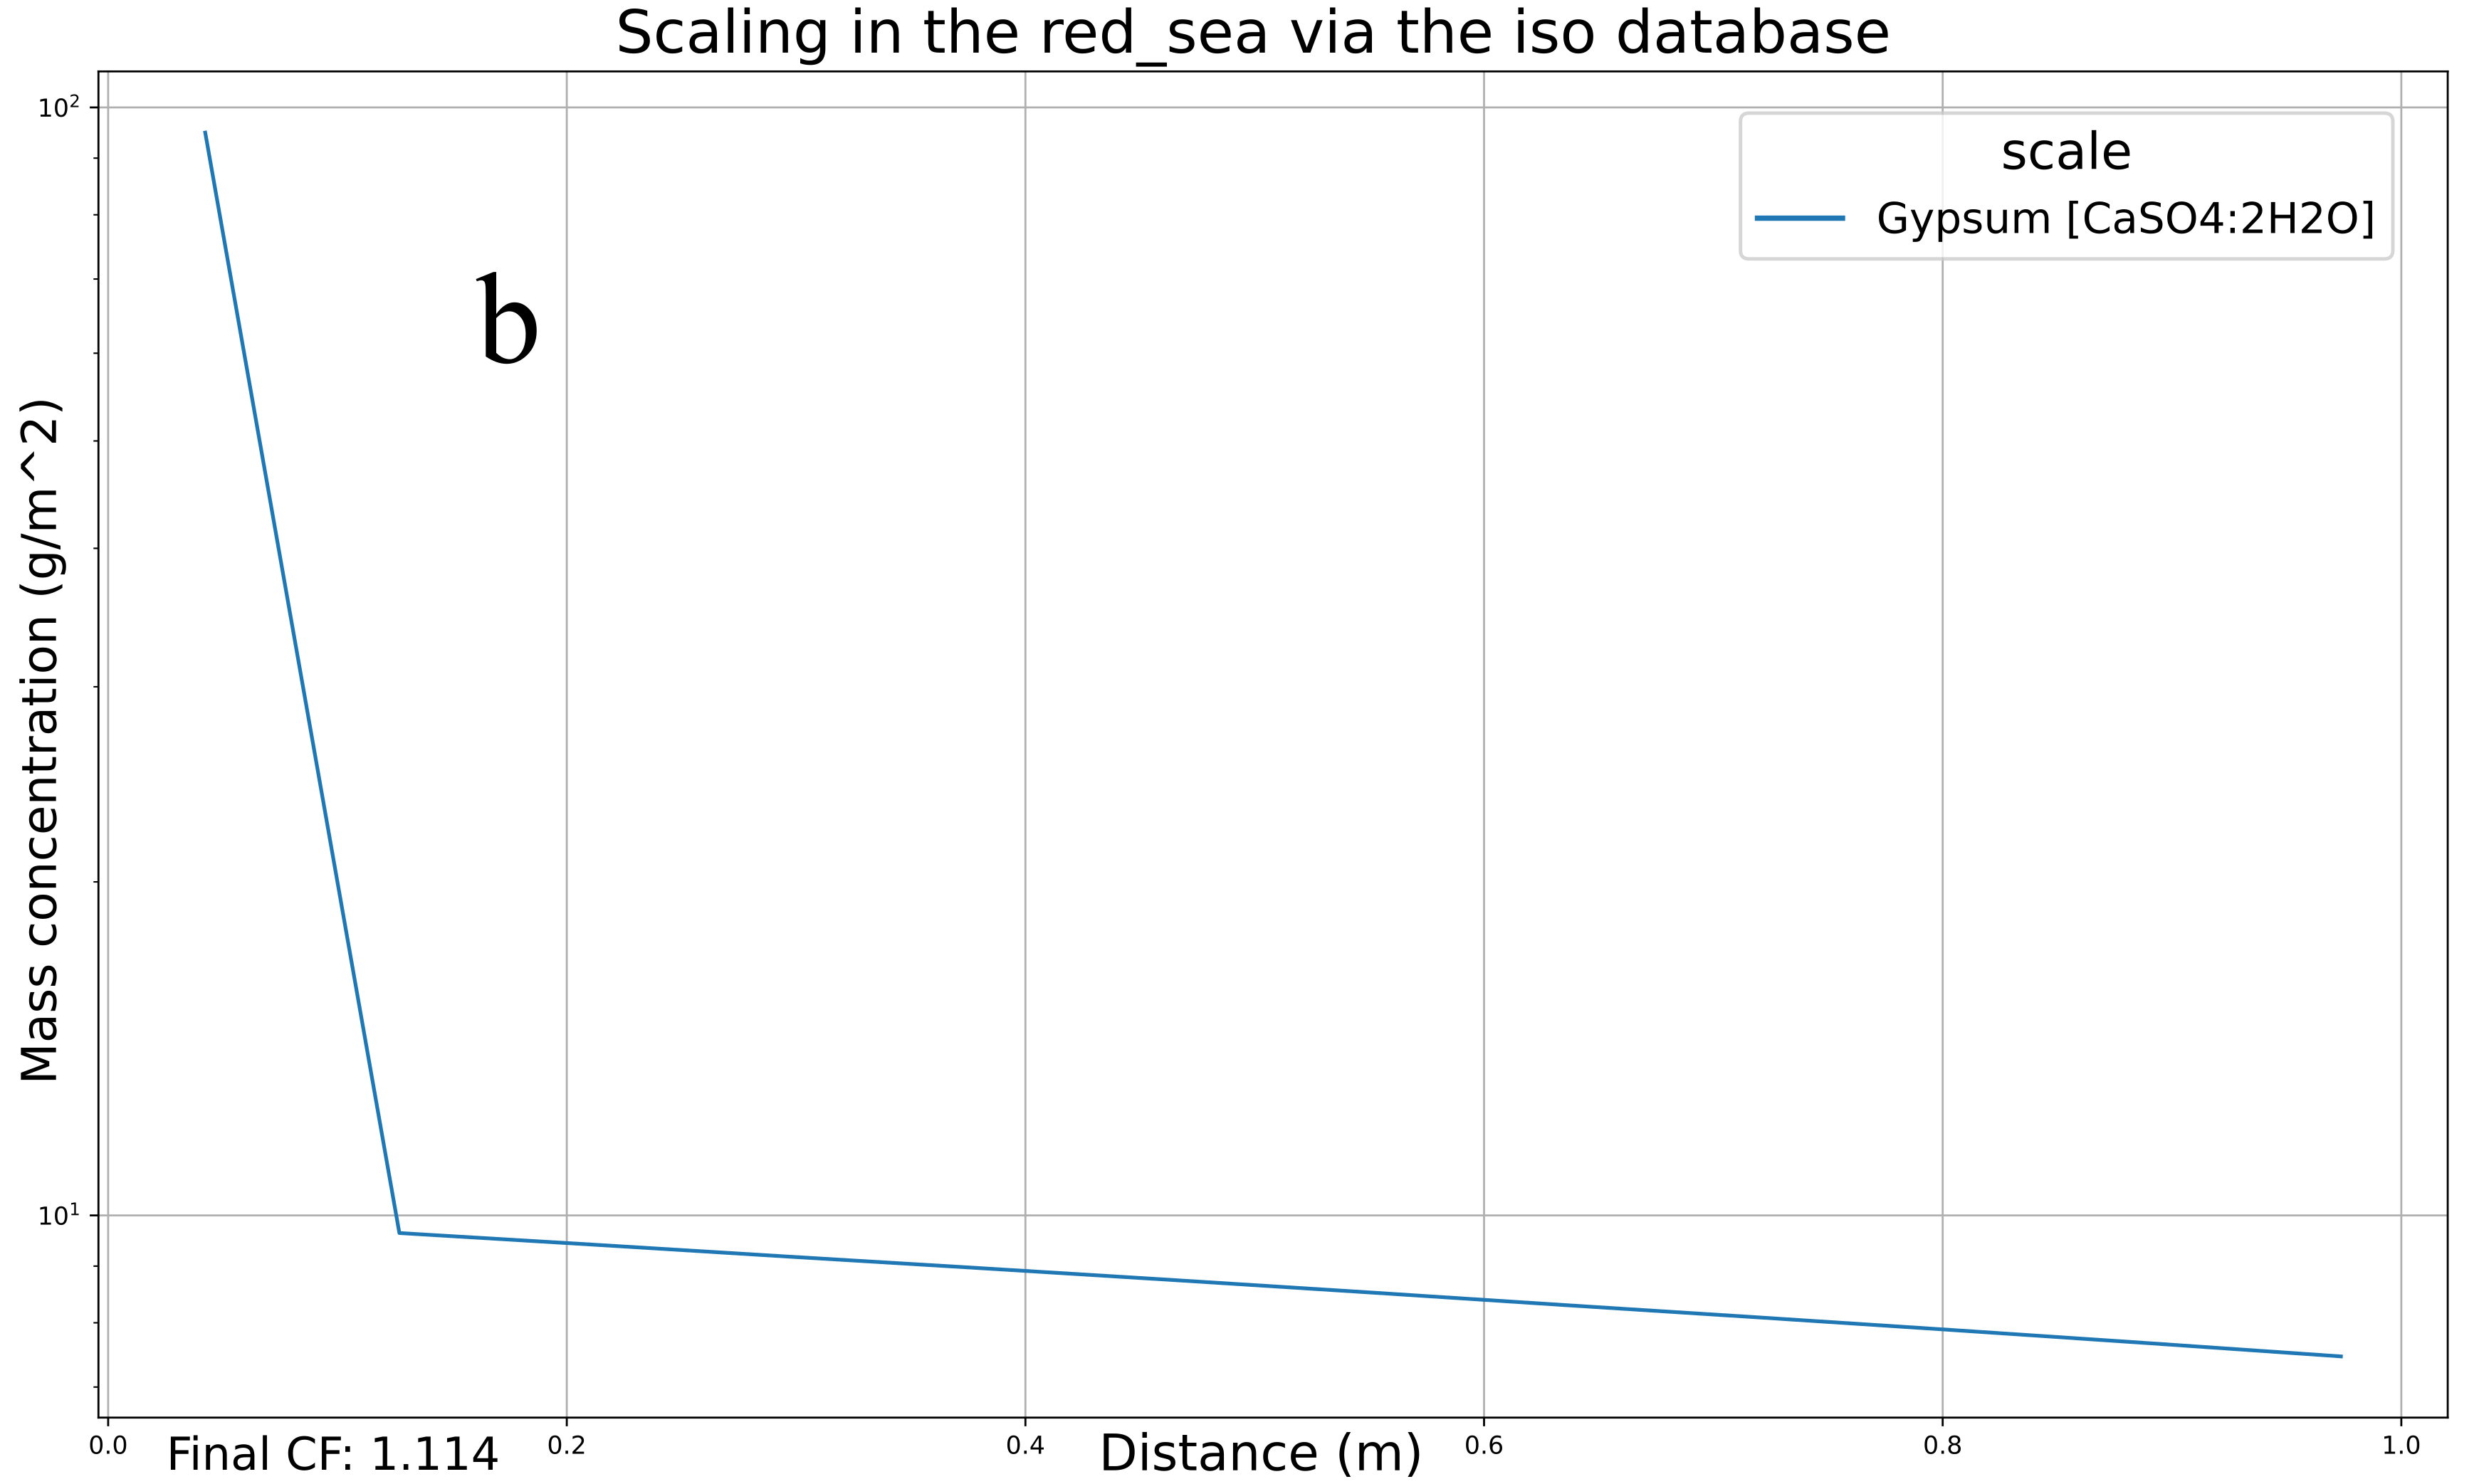
\includegraphics[width=0.49\textwidth]{images/ROSSpy/sensitivity_analyses/databases/Iso.png} \\ \midrule 
        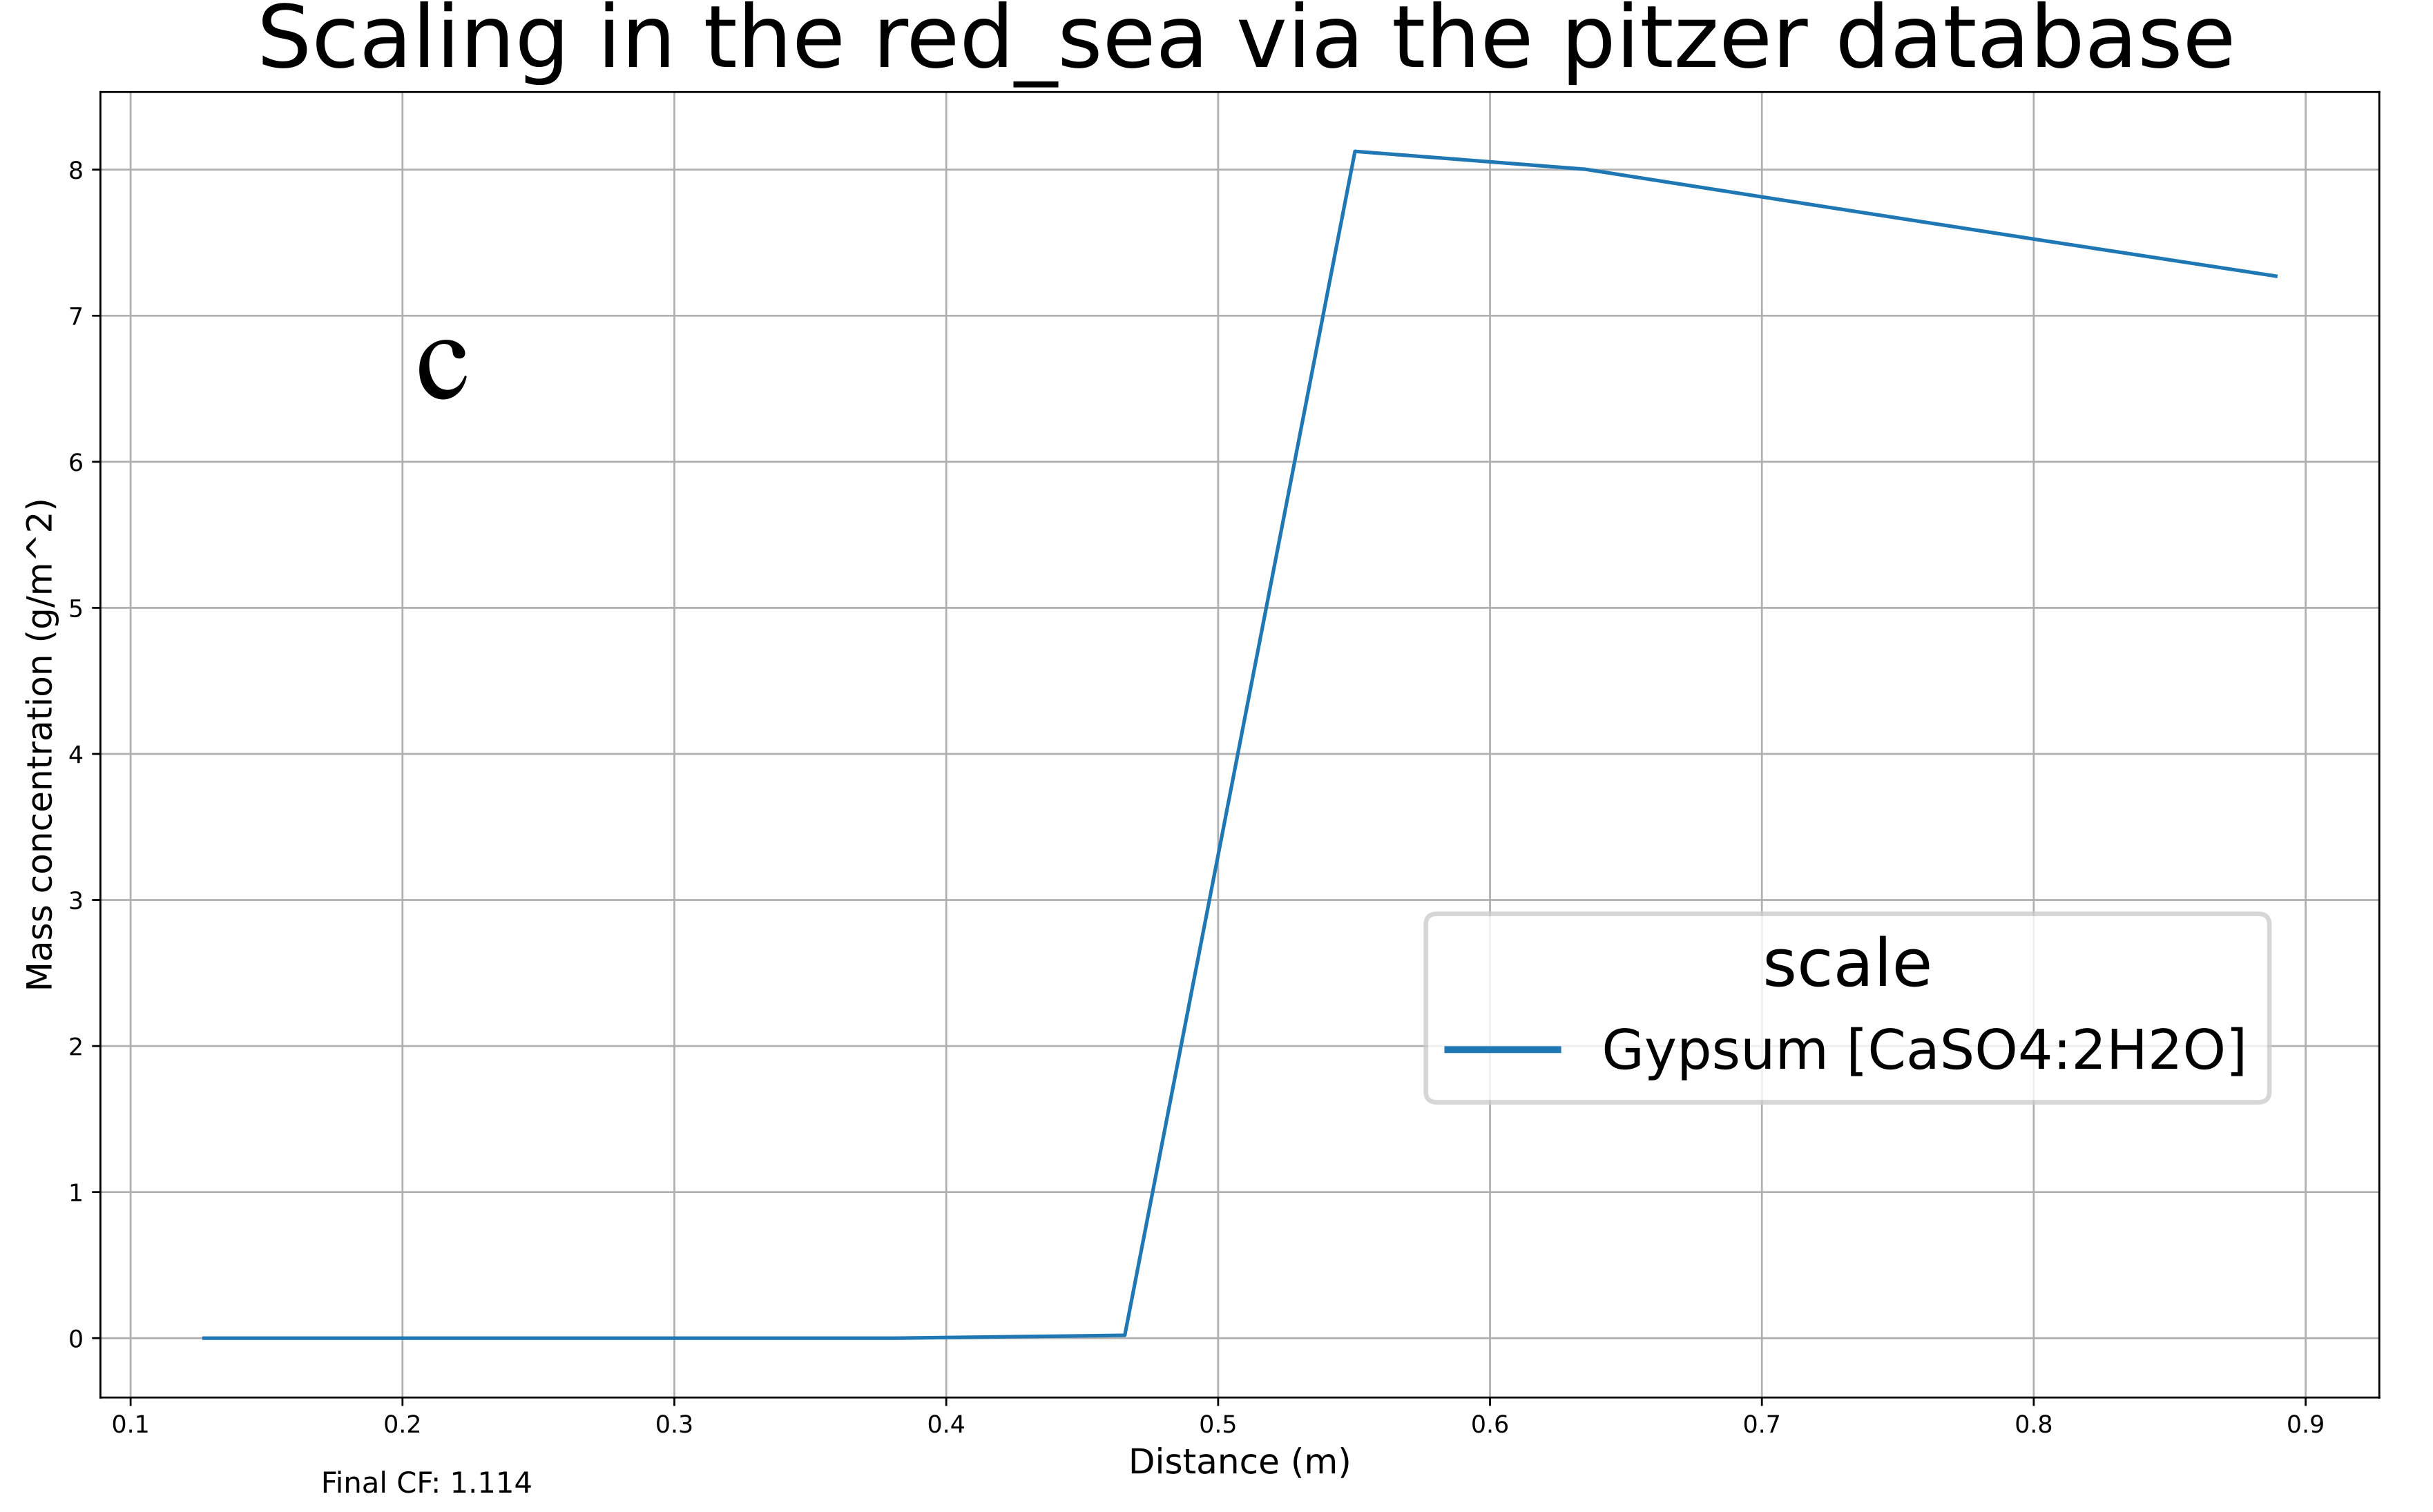
\includegraphics[width=0.49\textwidth]{images/ROSSpy/sensitivity_analyses/databases/Pitzer.png} 
        & 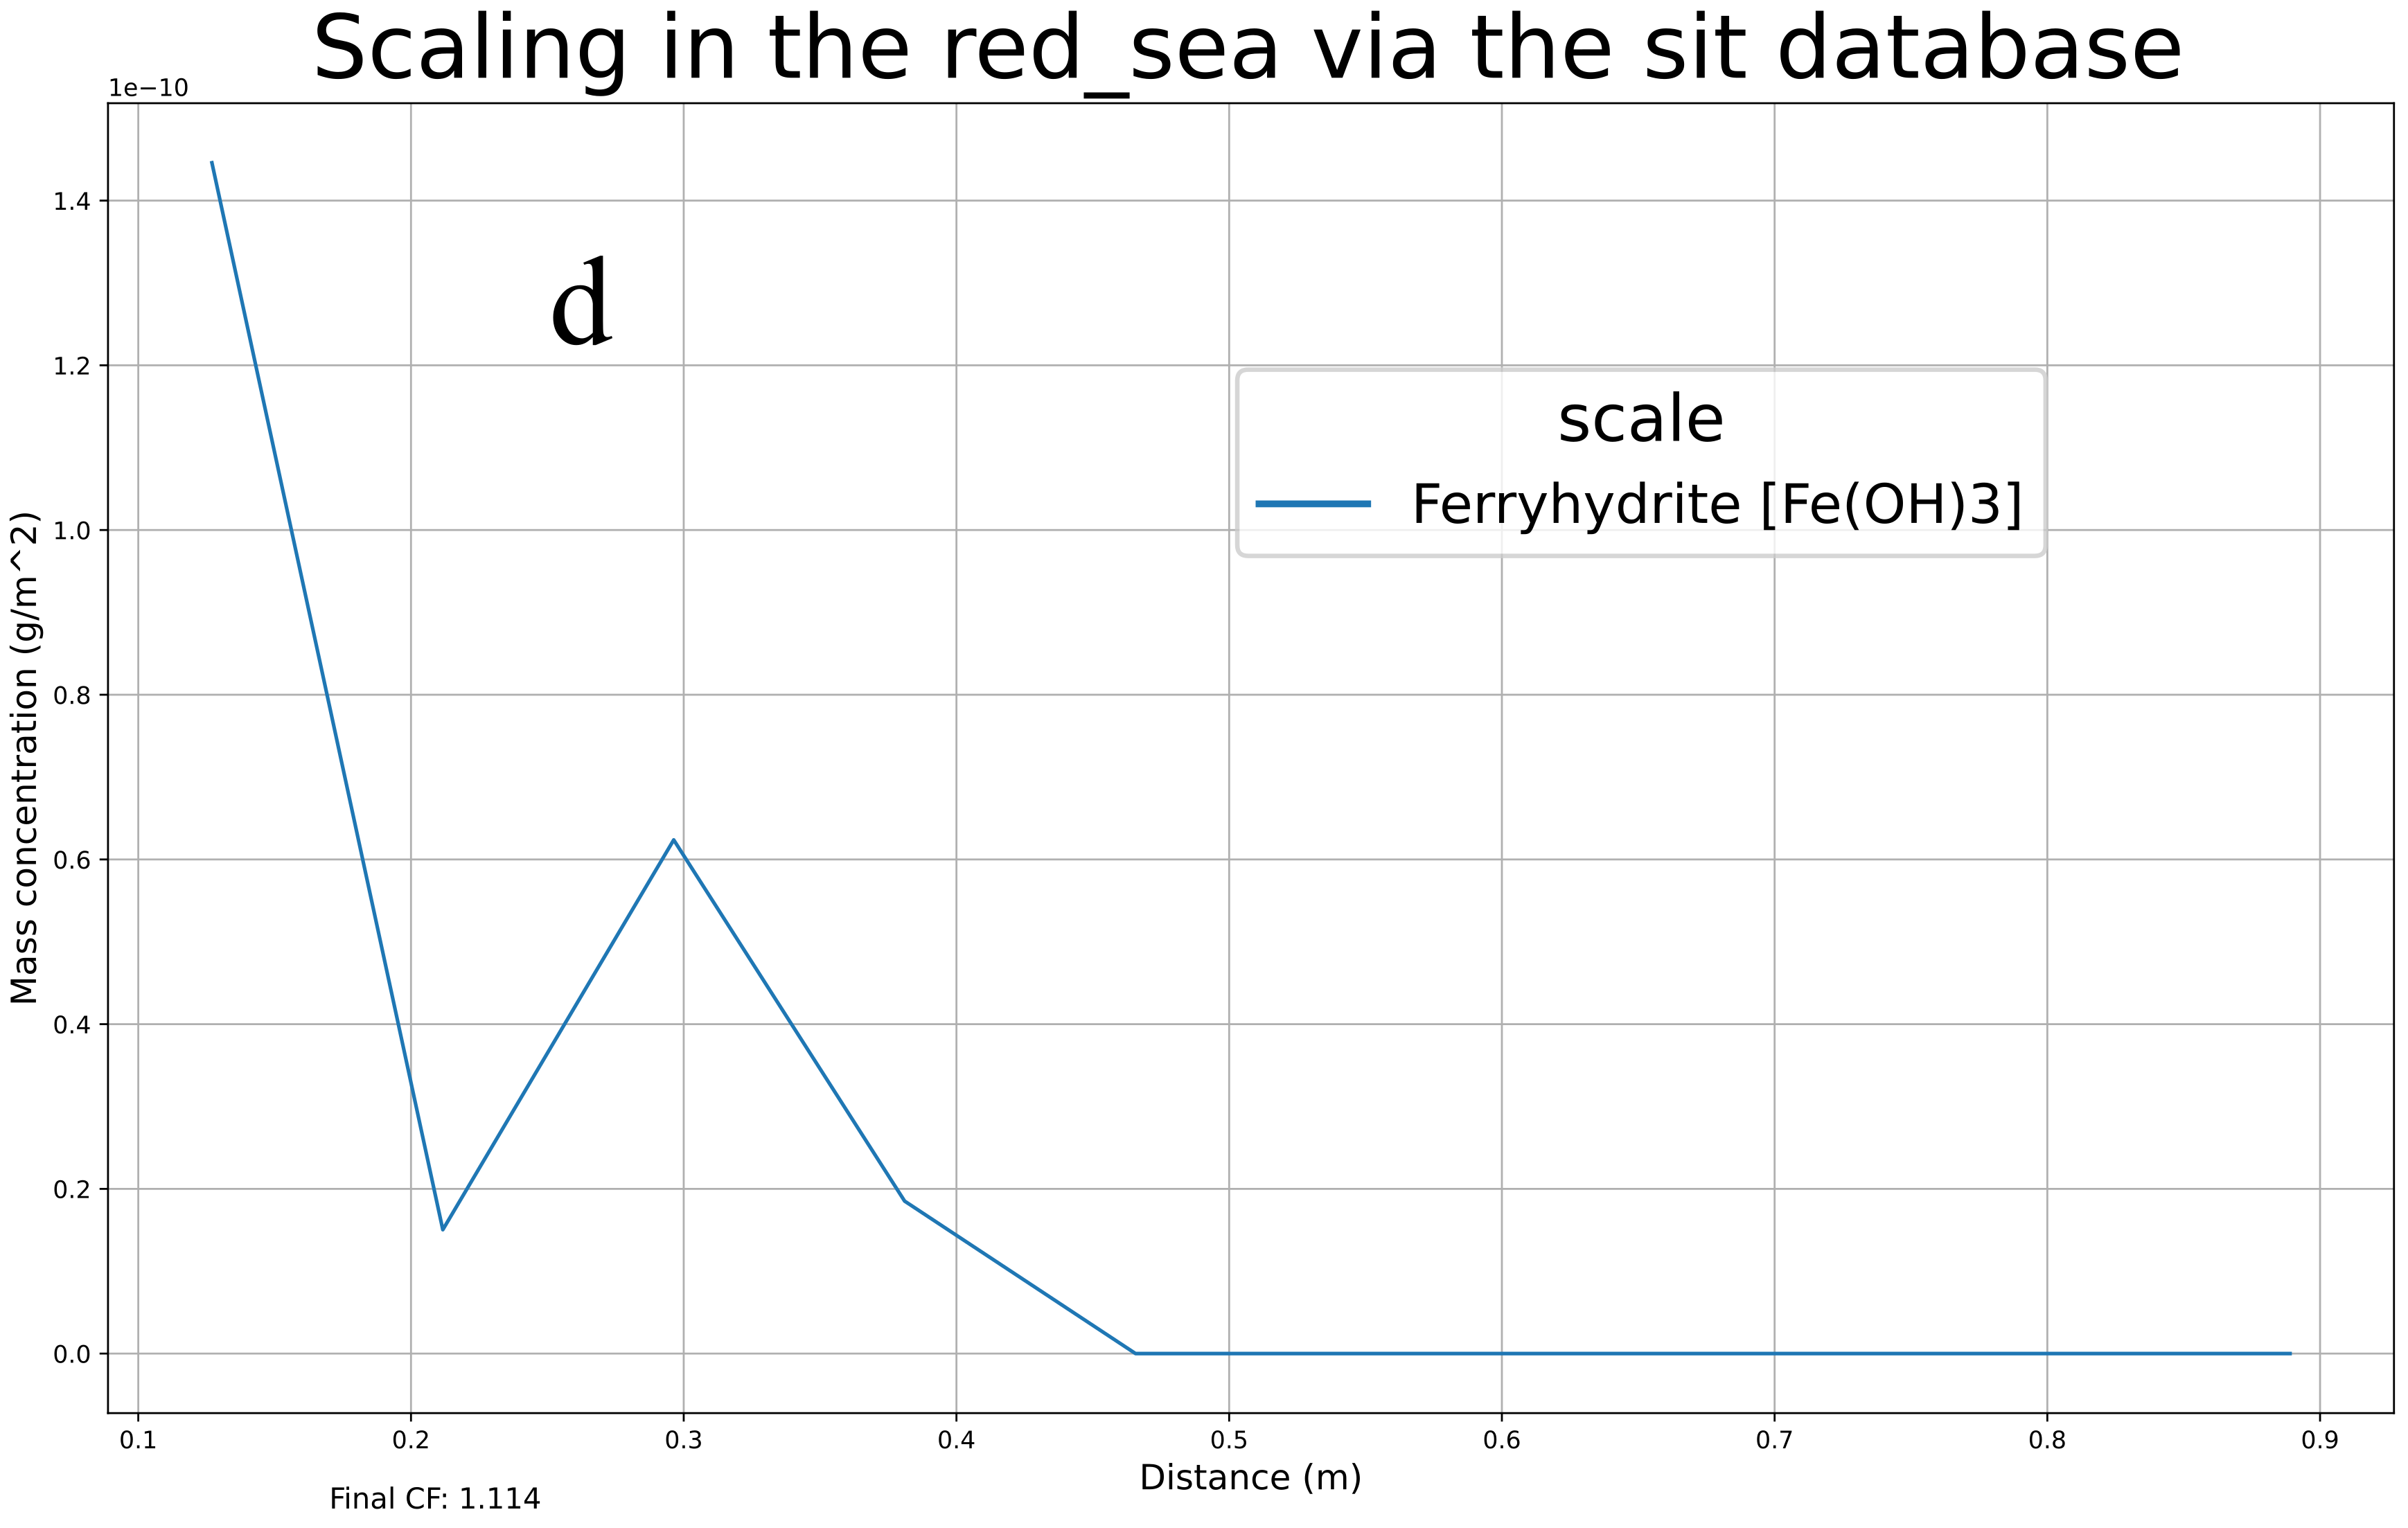
\includegraphics[width=0.49\textwidth]{images/ROSSpy/sensitivity_analyses/databases/Sit.png} 
        \\ \bottomrule
    \end{tabular}
    \caption{
        Scaling predictions from the a) ColdChem, b) Iso, c) Pitzer, and d) Sit databases, with otherwise identical simulation parameters. These subfigures represent the spectrum of similar yet distinct predictions of scaling during the database sensitivity analysis, and exemplify that the PHREEQC database should be deliberately selected after reviewing the PHREEQC documentation to discern which database is most appropriate for the feed geochemistry.
    }
    \label{database_selection}
\end{figure}

\subsection{Feed geochemistry}
The default feed waters were constructed from experimental geochemical literature into parameter files that are provided with ROSSpy. Users of ROSSpy are encouraged to simulate their own feed water while emulating the syntax of the default parameter files. We propose experimental data of numerous other water sources in Section 5 of the Supporting Information that can predicate feed water files; although, direct measurement of the simulated feed water is preferable to avoid significant influences of anthropogenic pollution \cite{Chen2008SourcesSea} and seasonality \cite{Sarthou2001SeasonalSea} in reported measurements. Thee default water sources, which include both natural seas and produced waters from oil wells, were contrasted in Figure \ref{feed_sources}, where the scaling and brine predictions differed significantly amongst these feed water sources. 

\begin{figure}
    \centering
    \begin{tabular}{c|c}
        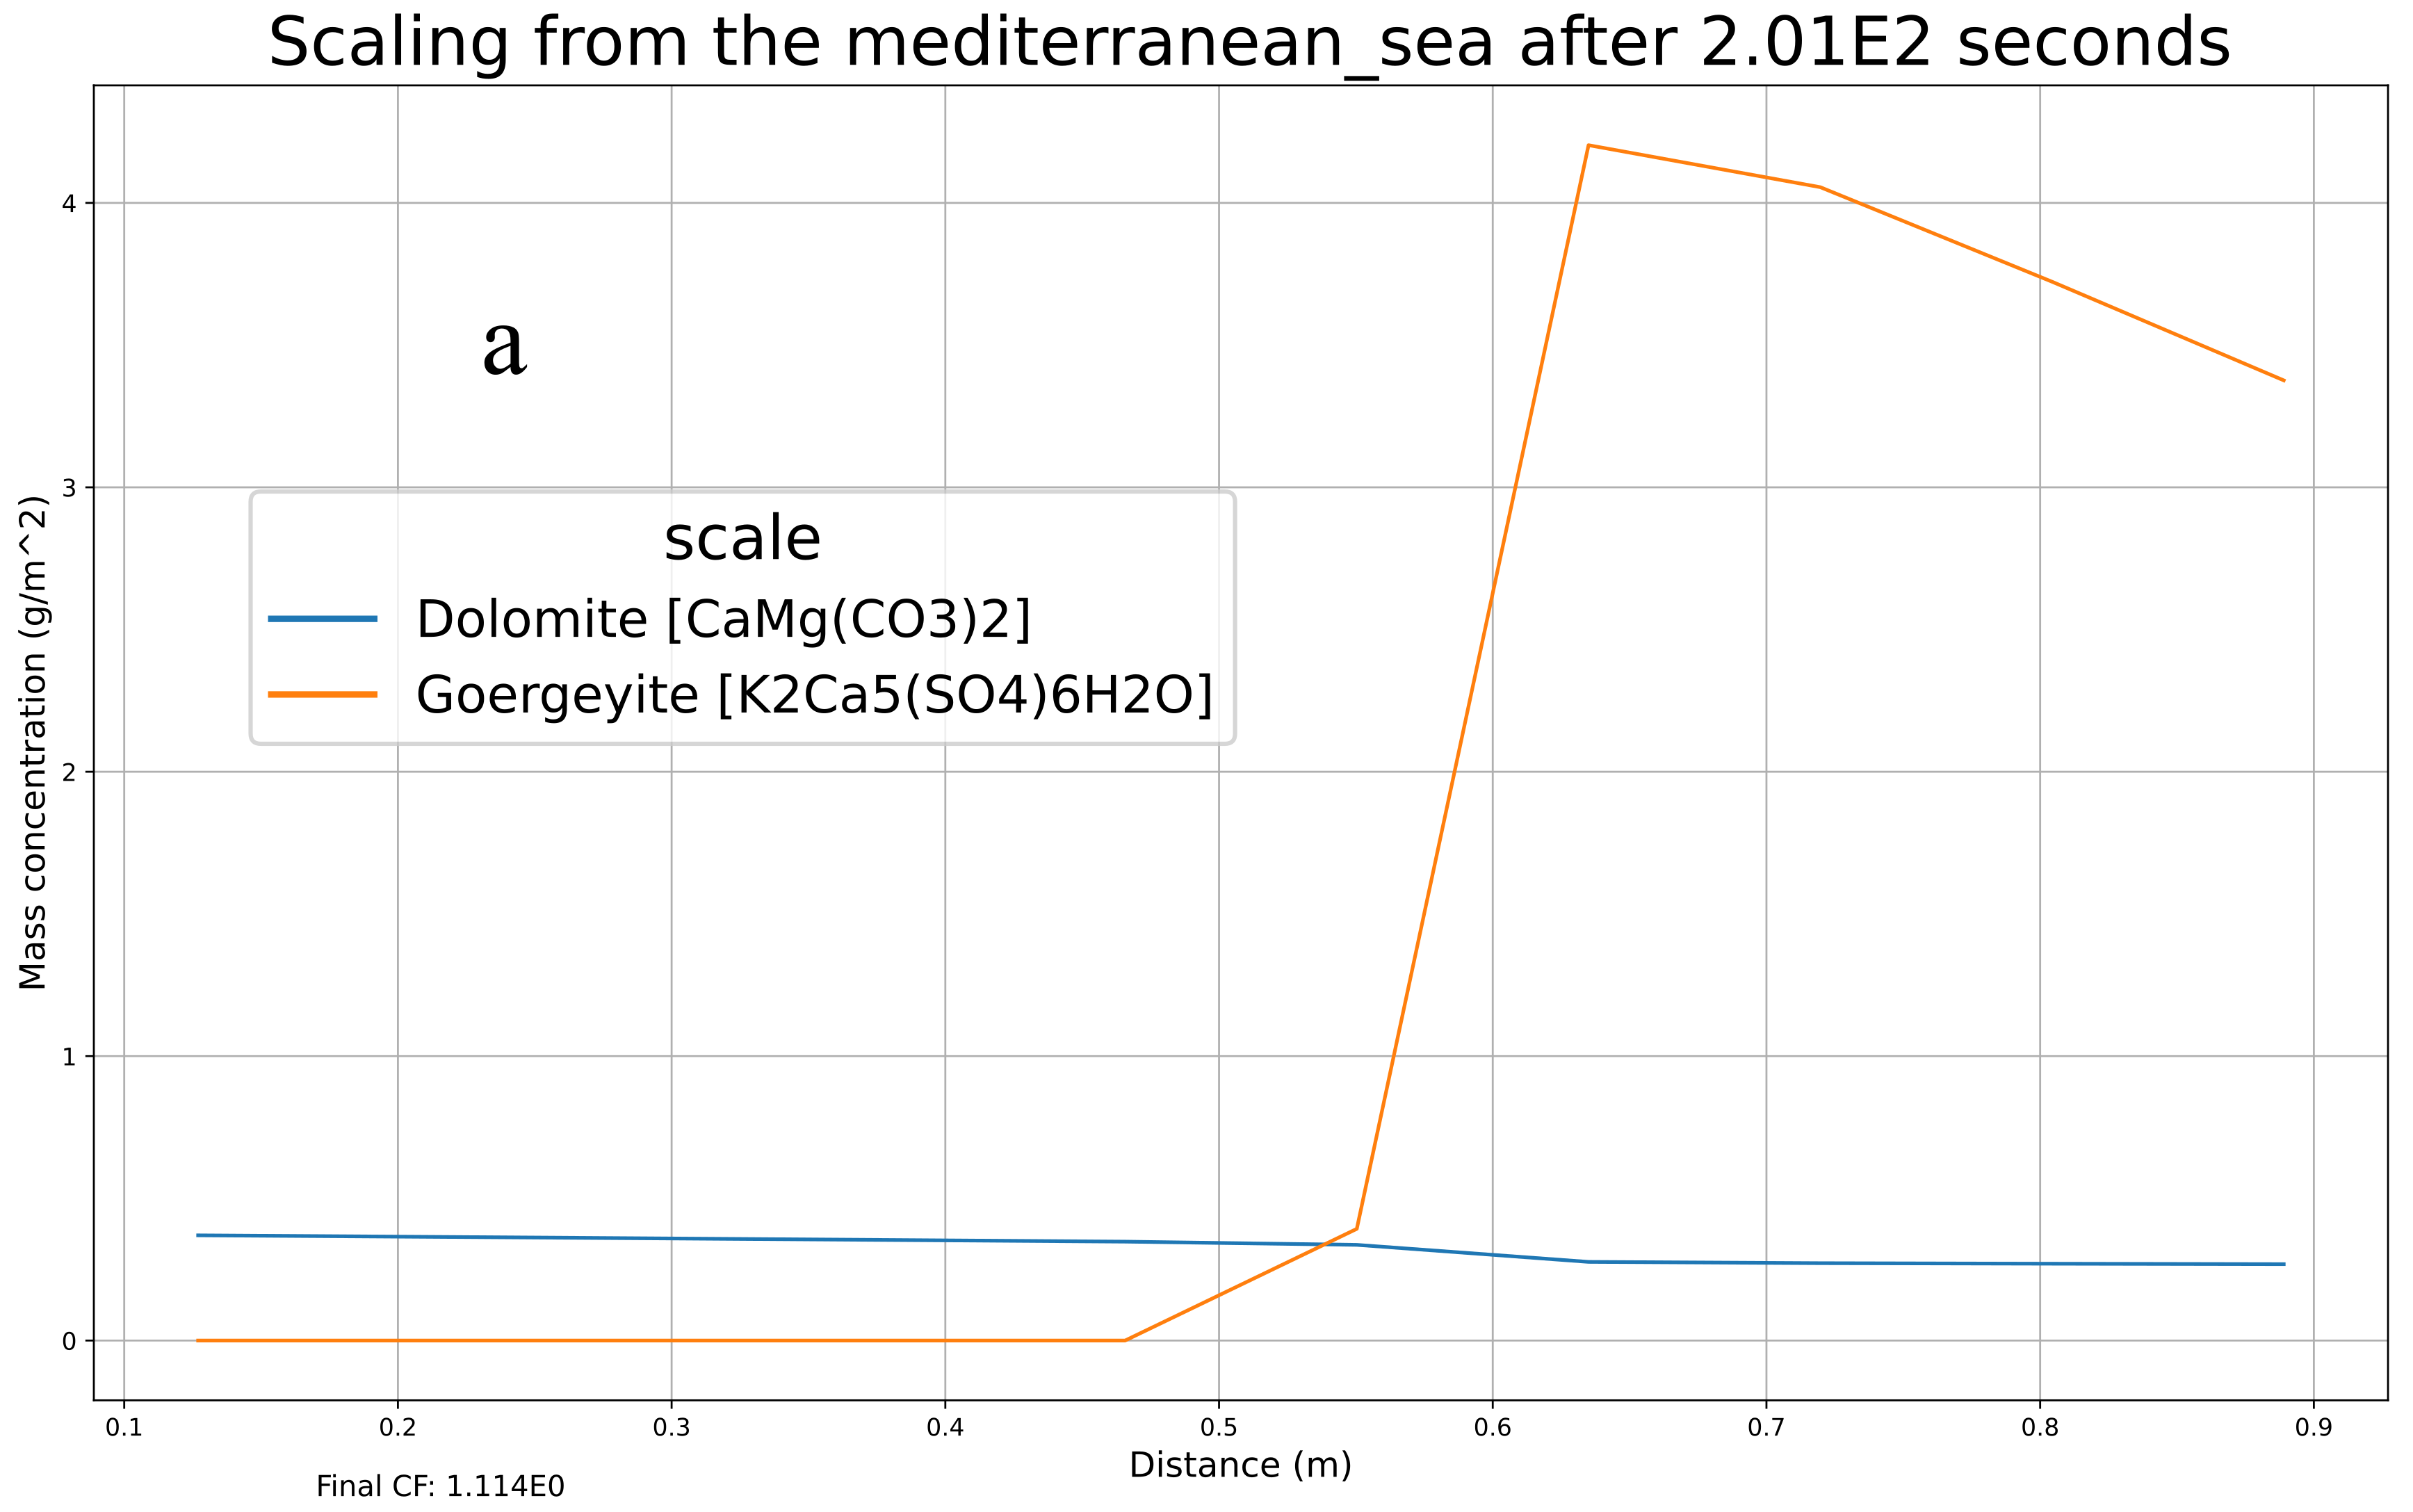
\includegraphics[width=0.49\textwidth]{images/ROSSpy/sensitivity_analyses/feed_source/Mediterranean.png} &
        \includegraphics[width=0.49\textwidth]{images/ROSSpy/sensitivity_analyses/feed_source/Palo_Duro_basin.png} \\ \midrule
        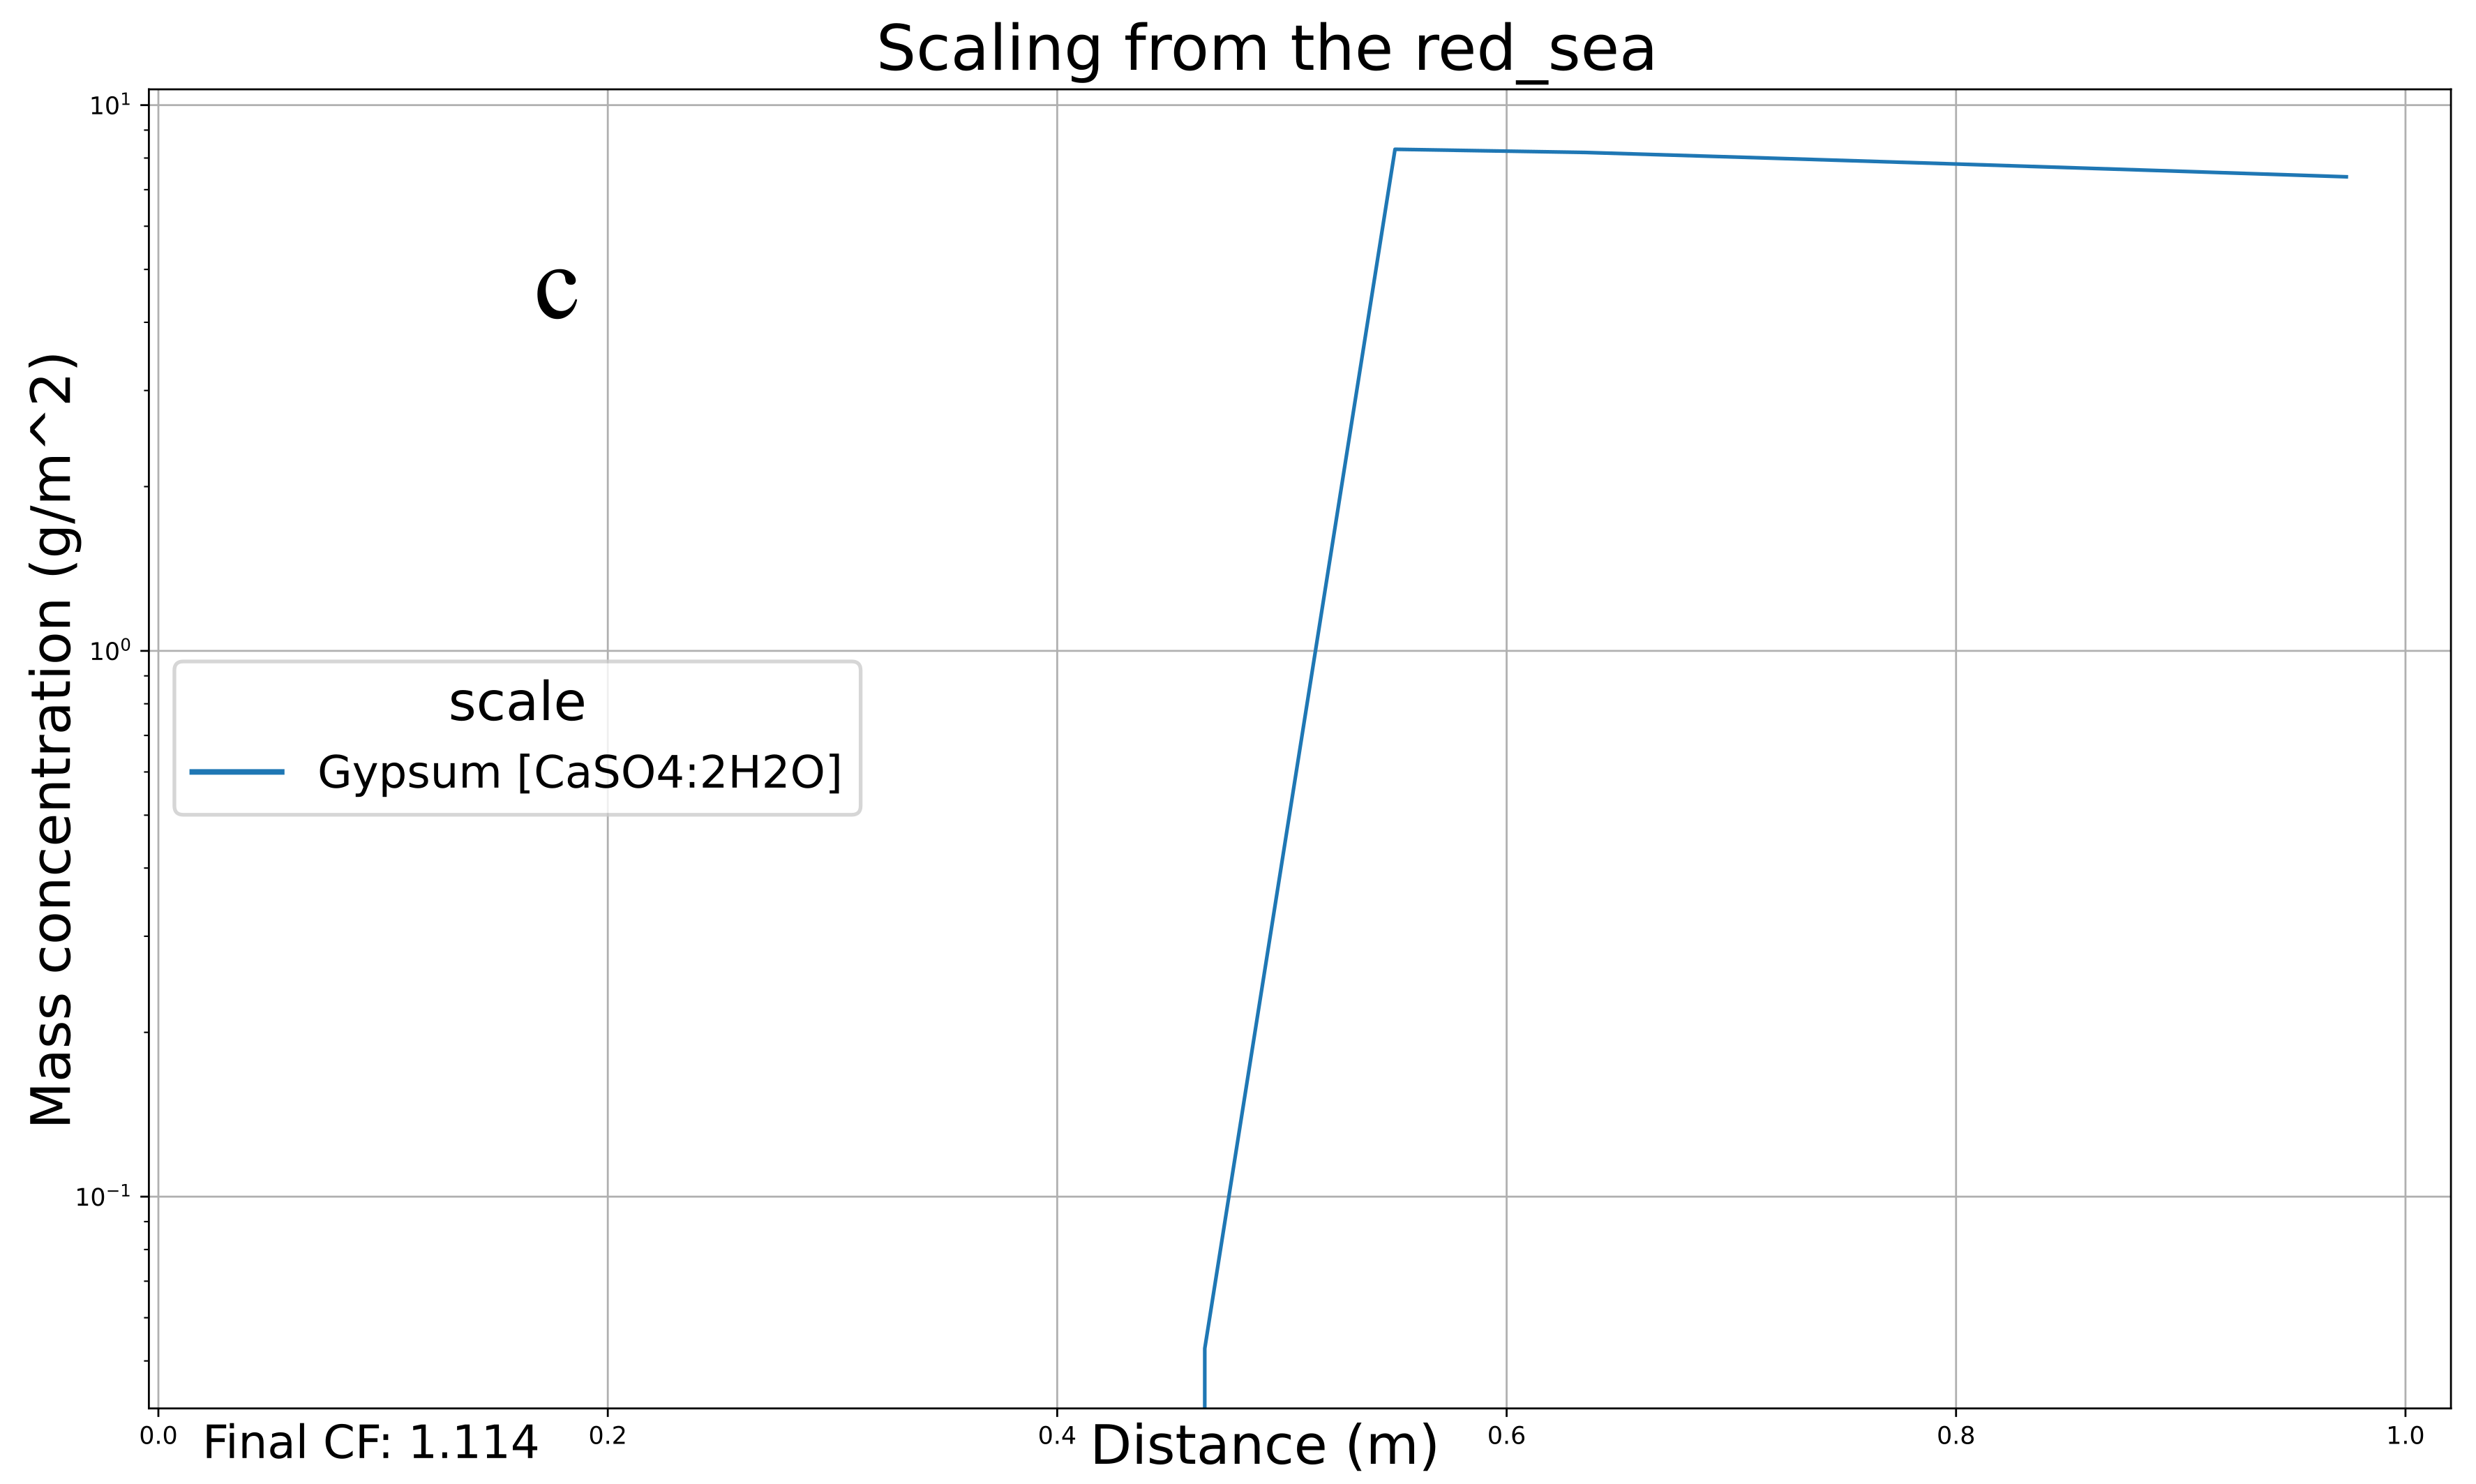
\includegraphics[width=0.49\textwidth]{images/ROSSpy/sensitivity_analyses/feed_source/Red_Sea.png} & 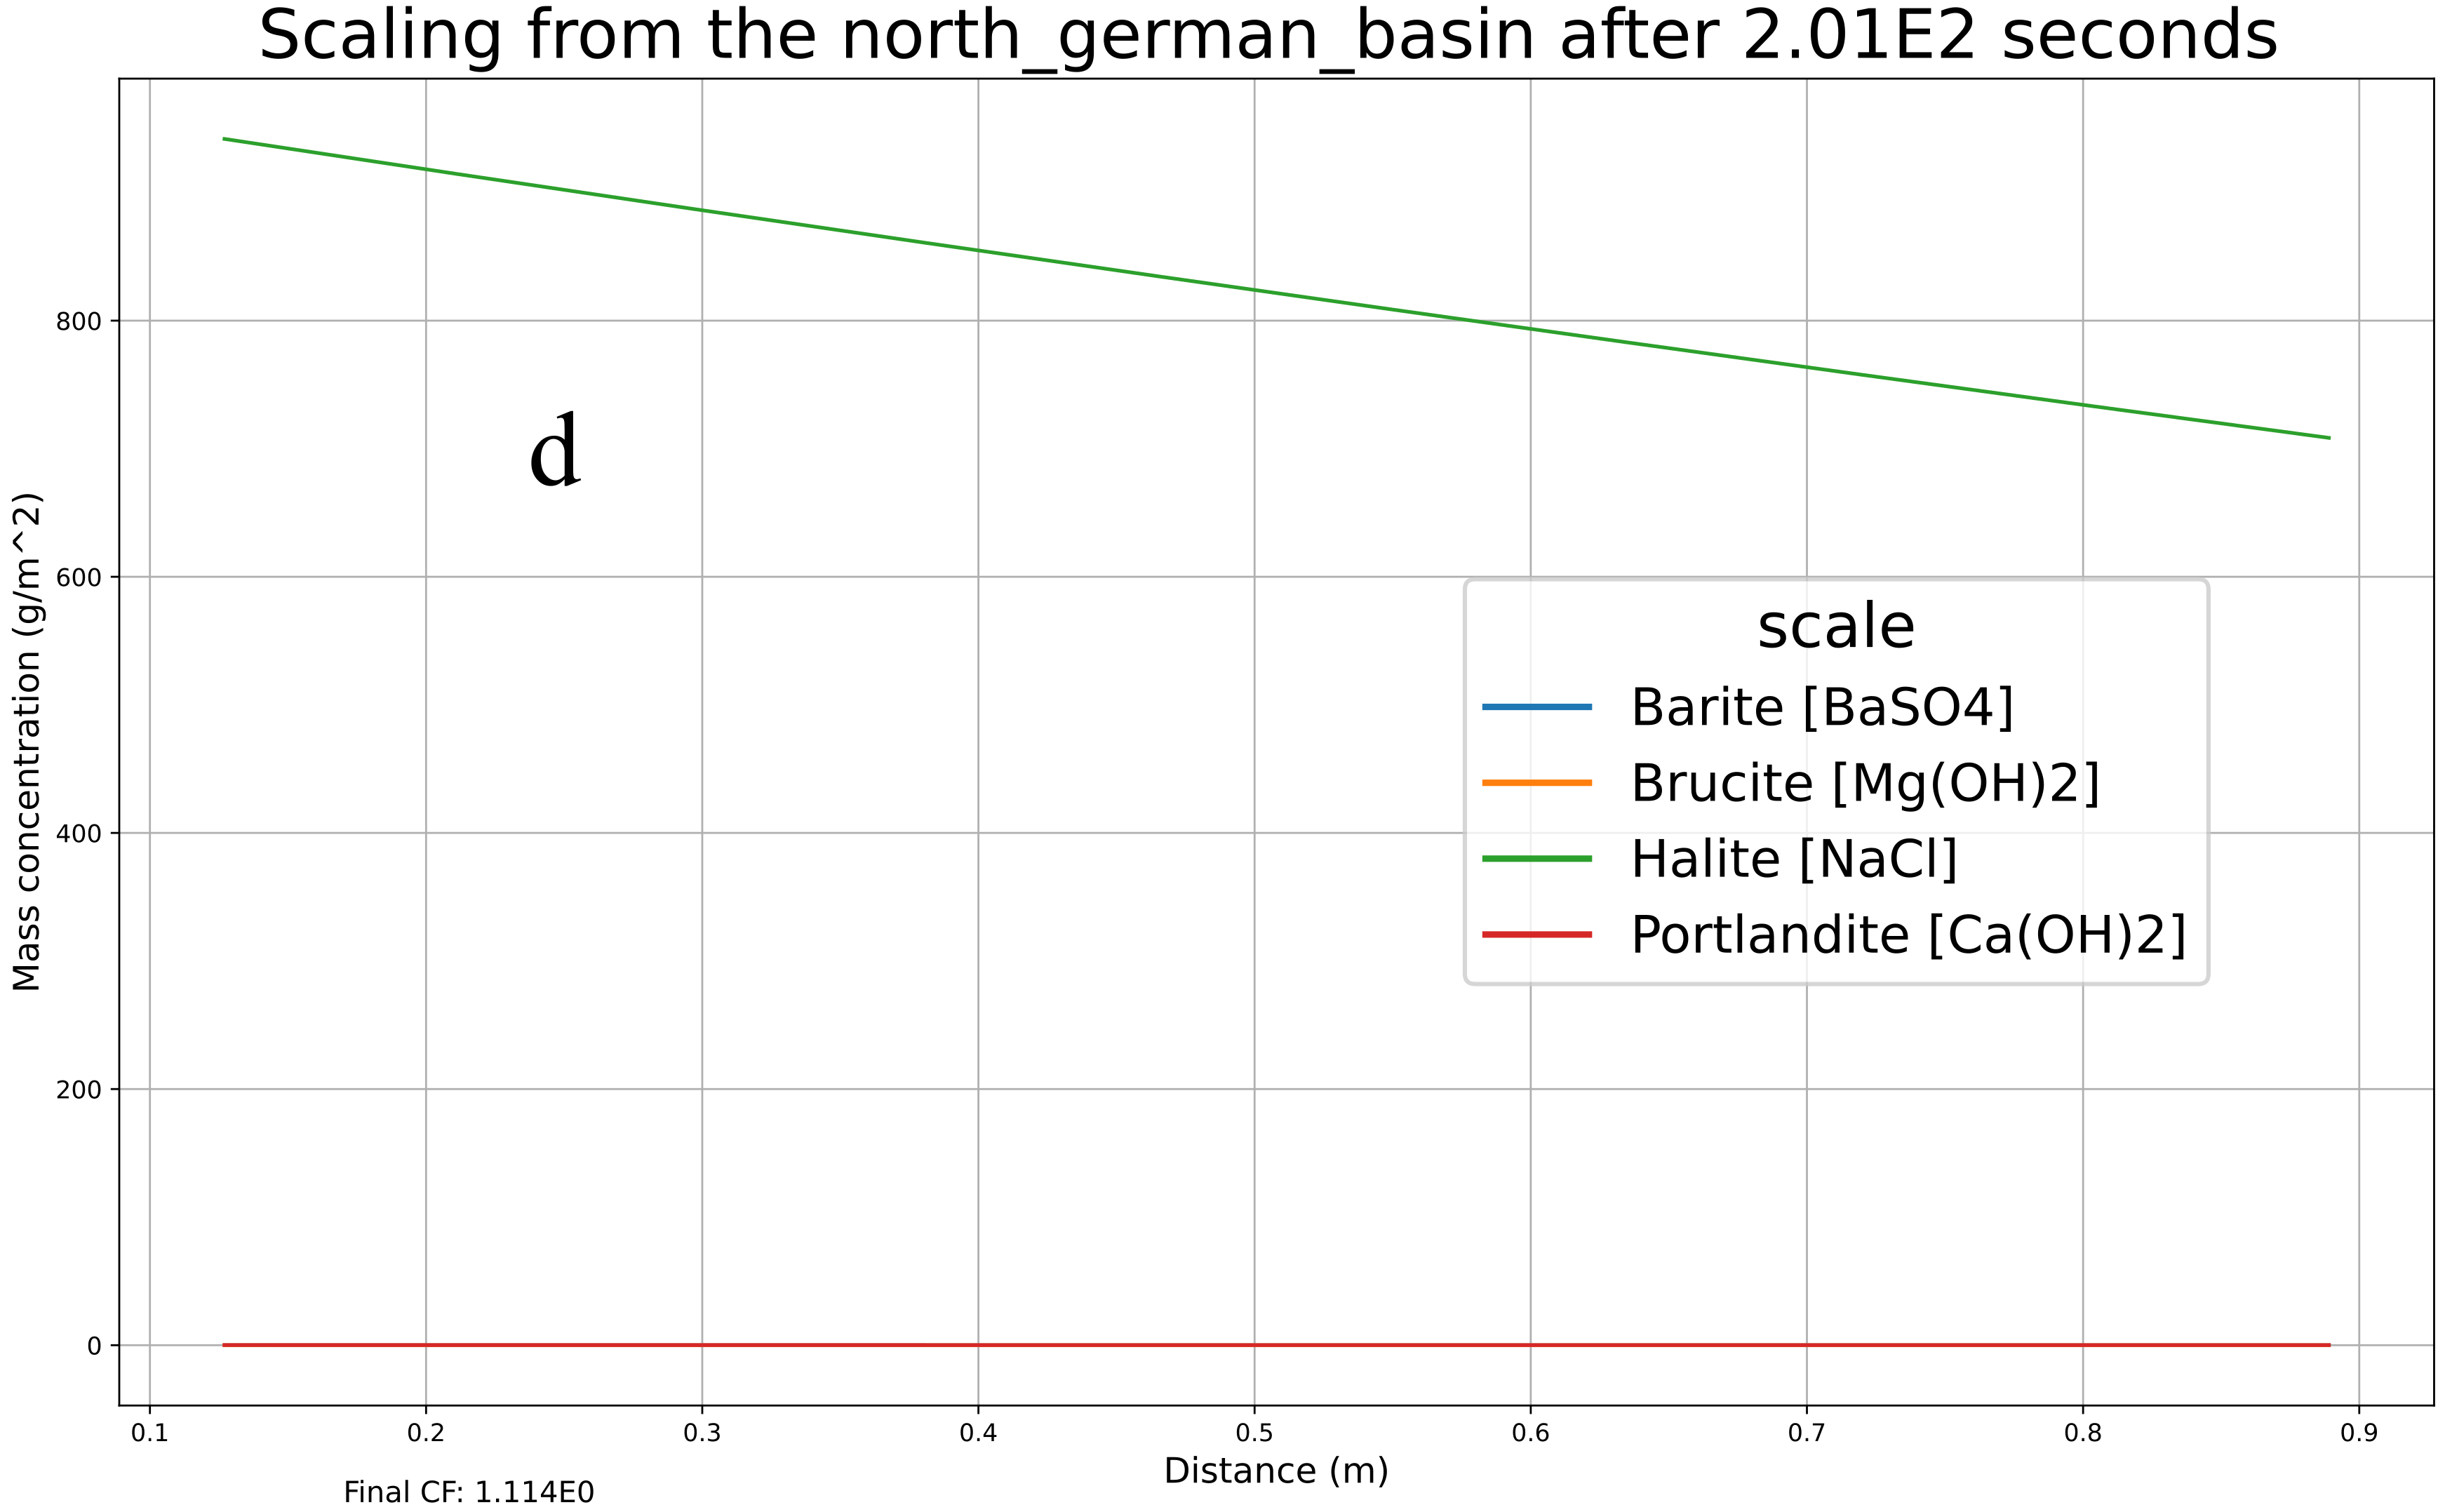
\includegraphics[width=0.49\textwidth]{images/ROSSpy/sensitivity_analyses/feed_source/German_Basin.png} \\ \bottomrule
    \end{tabular}
    \caption{
        Scaling predictions of a) the Mediterranean Sea, b) produced waters from the Palo Duro oil basin, c) the Red Sea, d) produced waters from the North German oil basin, with otherwise identical simulation parameters. These subfigures represent the spectrum of scaling predictions from the variety of different feed sources, which exhibits a high sensitivity of scale predictions to the feed geochemistry. 
    }
    \label{feed_sources}
\end{figure}

\section{Software}
ROSSpy, which is conceptualized by Figure \ref{workflow}, combines our one-dimensional RO model with post-processing operations that facilitate interpretation of the simulation results. The software a) translates parameters into a PHREEQ input file; b) executes that input file via PHREEQpy; c) processes the simulation results into figures and data tables via Matplotlib \cite{Hunter2007Matplotlib:Environment} and Pandas \cite{McKinney2011Pandas:Statistics} Python packages, respectively; and d) exports all of the simulation content -- e.g. the PHREEQ input file, SVG data figures, and CSV files of parameters, variables, data, and brine predictions -- into a specified folder and directory. The simulation data may be sliced into one-dimensional sets of distance or time that can be plotted against either scaling density or brine concentrations (Figures S2-S3) (see ROSSpy documentation).


\begin{figure}
    \centering
    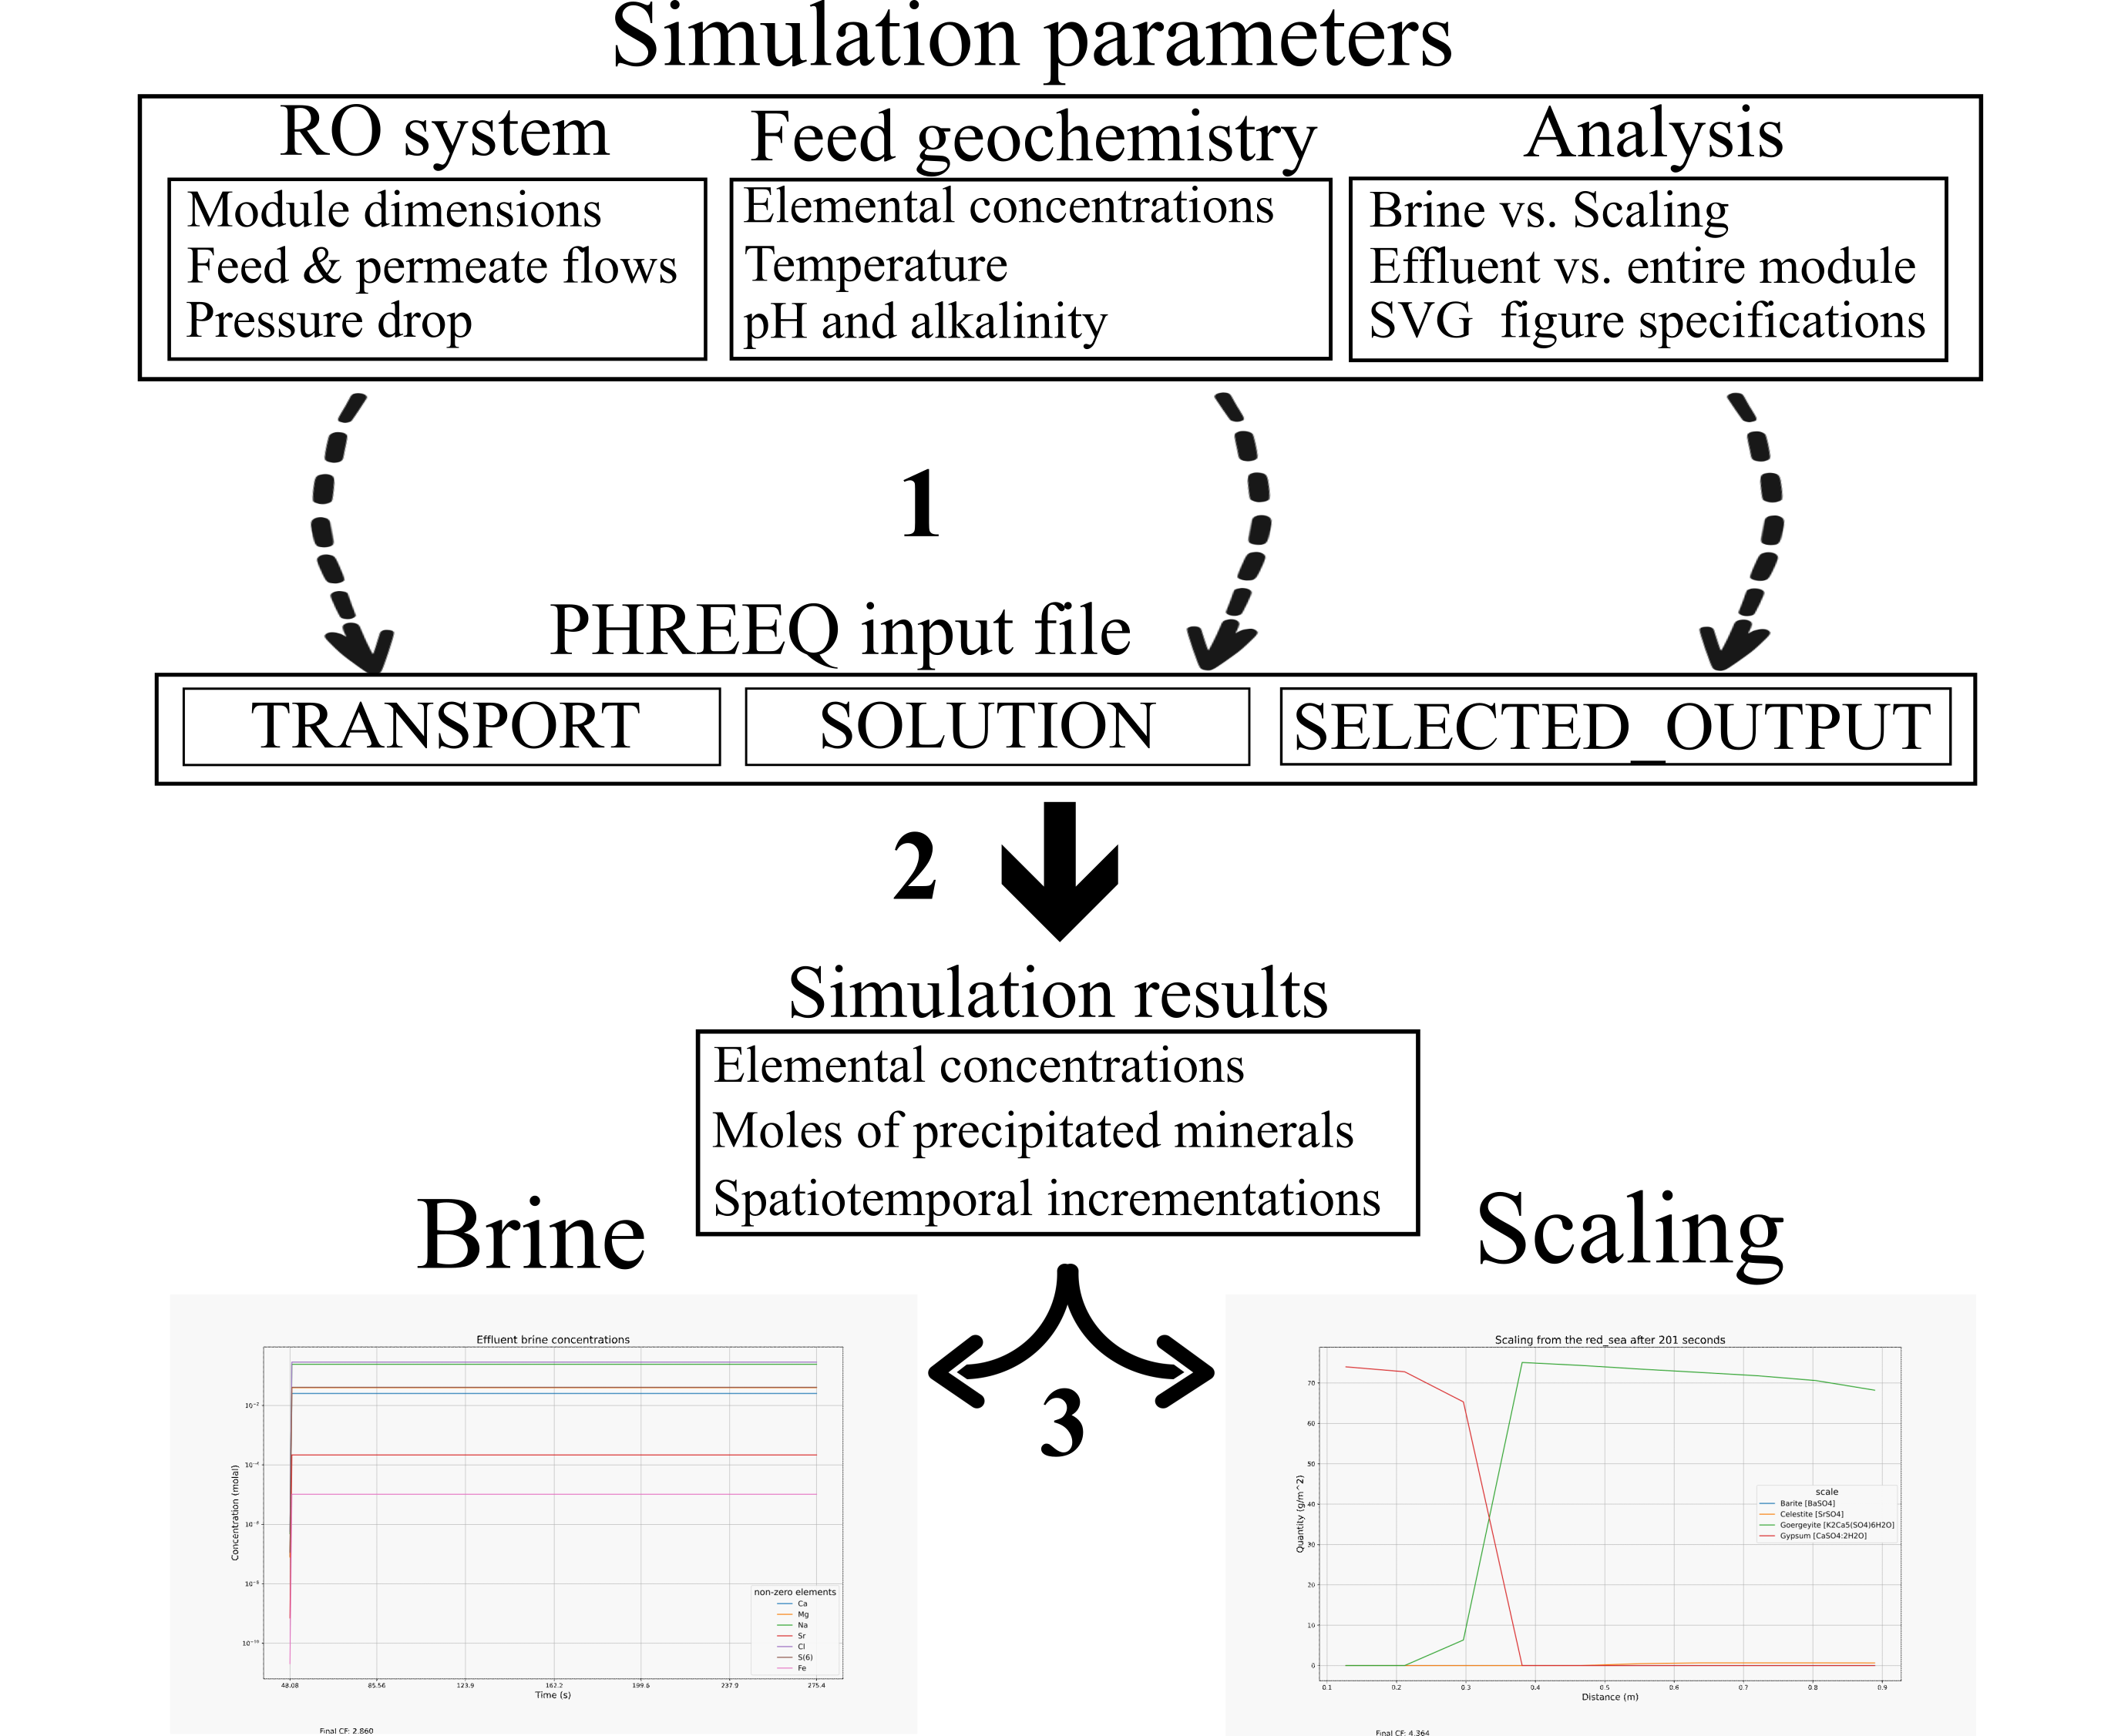
\includegraphics[width = \linewidth]{images/ROSSpy/rosspy_workflow_1.PNG}
    \caption{
        The ROSSpy workflow. Step 1 describes the translation of parameters -- i.e. module specifications, feed geochemistry, and simulation analysis -- into the corresponding code blocks of a PHREEQ input file. Step 2 describes executing the PHREEQ input file via either PHREEQpy in ROSSpy, or via the PHREEQC batch software in the interactive version of ROSSpy (iROSSpy) that is under development. Step 3 describes processing the predictions of brine concentrations or scaling quantities into representative figures and datatables, which are ultimately exported.
    }
    \label{workflow}
\end{figure}

\section{Conclusion}

A one-dimensional approximation of RO reactive transport geochemistry, executed in PHREEQC, is a practical and accurate representation of mineral scaling during desalination. The simulation predictions of this model were quantitatively and qualitatively verified for a few use cases, with both theoretical expectations and experimental data where it was available. The API implementation of this model (ROSSpy) furthermore meets identified needs of the community -- e.g. rapidly designing, executing, processing, and exporting simulations of RO scaling -- while maintaining accessibility through its light-weight design and its open-source code. We expect that this one-dimensional model and the unique attributes of ROSSpy  will facilitate scaling research and ultimately improve the efficiency of RO desalination towards alleviating chronic water insecurities in the world. 

\section{Funding}
This work was prepared in partial fulfillment of the requirements of the Berkeley Lab Undergraduate Research (BLUR) Program, managed by Workforce Development \& Education at the Berkeley Lab. The project was also partly funded by NSERC Discovery, MITACS Accelerate, CEWIL, and Canada Summer Jobs. 

% Acknowledgements section
\section{Acknowledgement}
The authors thank Ethan Sean Chan for his technical assistance in developing a graphical interface of ROSSpy (iROSSpy) that will be released in a future version. 
\newpage


% \layout
%     \setlength{\hoffset}{0pt}
%     \setlength{\voffset}{0pt}
%     \setlength{\topmargin}{0pt}
%     \setlength{\oddsidemargin}{0pt}
%     \setlength{\marginparwidth}{0pt}
%     \setlength{\marginparsep}{0pt}
%     \setlength{\textwidth}{465pt}
%     \setlength{\textheight}{600pt}
% \layout*


\section{Supporting Information}

\begin{supplementary}

\subsection{ROSSpy}

The variables and terms that comprise our model are defined in Table \ref{glossary}.

\begin{longtable}{c|c|c}
    \caption{
        Glossary of ROSSpy variables.  
        \label{glossary} 
    } \\ \toprule
    
    \textbf{variable} & \textbf{name} & \textbf{description} \\ \toprule
    \endfirsthead
    \multicolumn{3}{c}{continuation of Table \ref{glossary}} \\  \toprule
    \textbf{variable} & \textbf{name} & \textbf{description} \\ \toprule
    \endhead
    
    \multirow{2}{1.5em}{$l$} & \multirow{2}{3em}{length} & longitudinal dimension of the\\& & module or module cell \\ \midrule
    \multirow{2}{1.5em}{$n$} & number of & quantity of discretizations of the module \\ & module cells & \\ \midrule
    $\Phi_e$ & moles & the $moles_{H_2O}$ that exist in cell $e$ \\ \midrule  
    $\Delta \Phi_e$ & permeate flux & the $moles_{H_2O}$ that are removed in cell $e$ \\ \midrule  
    $HL$ & head loss & reduction of pressure over the module distance \\ \midrule
    \multirow{2}{2em}{$PE$} & \multirow{2}{3em}{permeate efficiecy} & attenuation of permeate flux \\& & from pre-existing inefficiencies \\ \midrule  
    \multirow{2}{2em}{$CF$} & \multirow{2}{3em}{concentration factor} & solution concentration of cell $e$ normalized \\& & to the influent concentration \\ \midrule
    $X$ & mass & water mass in the maximally filled feed channel \\ \midrule
    $V$ & velocity & feed velocity through the feed channel \\ \midrule
    $A$ & area & cross-sectional area of the RO module \\ \midrule
    $th$ & thickness & thickness of a module dimension \\ \midrule
    $Q$ & volumetric flow & feed flow through a maximally filled feed channel \\ \midrule
    \multirow{2}{1.5em}{$\Delta t$} & \multirow{2}{3em}{time} & timestep of the simulation that \\& & adheres to the Courant condition \\ \midrule
    \multirow{2}{2em}{$C_{max}$} & \multirow{2}{3em}{Courant constant} & maximal value of the Courant constant \\& & to meet the Courant condition \\ \midrule
    $\phi$ & total concentration & total ionic concentrations in the simulation \\ \midrule
    $C$ & specie concentration & concentration of an individual specie \\ \midrule
    \multirow{2}{1em}{$v$} & \multirow{2}{3em}{stoichiometry coefficient} & coefficient for the respective compound \\& & in the balanced equilibrium reaction \\ \midrule
    \multirow{2}{1em}{$N$} & number of & quantity of reactions that \\& reactions & contain a respective compound \\ \midrule
    $R$ & reaction flux & $\frac{mmol}{hour}$ flux of an equilibrium reaction \\ \midrule
    \multirow{2}{1em}{$\Omega$} & thermodynamic & logarithm of the $\frac{Q_{dissolution}}{K_{sp}}$ \\& displacement & \\ \midrule
    $k_m$ & rate constant & dissolution and precipitation rate constant \\ \midrule
    $a$ & activity & chemical activity of the respective compound \\ \midrule
    $\eta$ \& $p$ & parameter & experimentally determined parameter \\ \midrule
    \multirow{2}{2em}{$\Delta G$} & \multirow{2}{5em}{Gibbs free energy} & Gibbs free energy of the dissolution \\& & and precipitation reactions \\ \midrule
    $K$ & equilibrium constant & thermodynamic equilibrium of the respective reaction \\ \midrule
    $M$ & number of minerals & quantity of minerals in the studied system \\ \midrule
    $\gamma$ & activity coefficient & coefficient of metabolite activity in a respective system \\ \midrule
    $z$ & charge & compound charge of the respective metabolite \\ \midrule
    $\mu$ & ionic strength & charge-weighted concentration of a solution \\ \midrule
    $A$ \& $B$ & parameter & experimentally determined parameter \\ \midrule
    $a_j$ \& $b_j$ & fitted parameter & geochemical parameter that is fit to the system \\ \midrule
    $W_{aq}$ & water mass & mass of water in the system \\ \bottomrule
\end{longtable} 

The distinctions between slicing the simulation data through time or module distance is exhibited with brine in Figure \ref{brine_perspectives} and scaling in Figure \ref{scaling_perspectives}, respectively.

\begin{figure}
    \centering
    \begin{tabular}{c}
        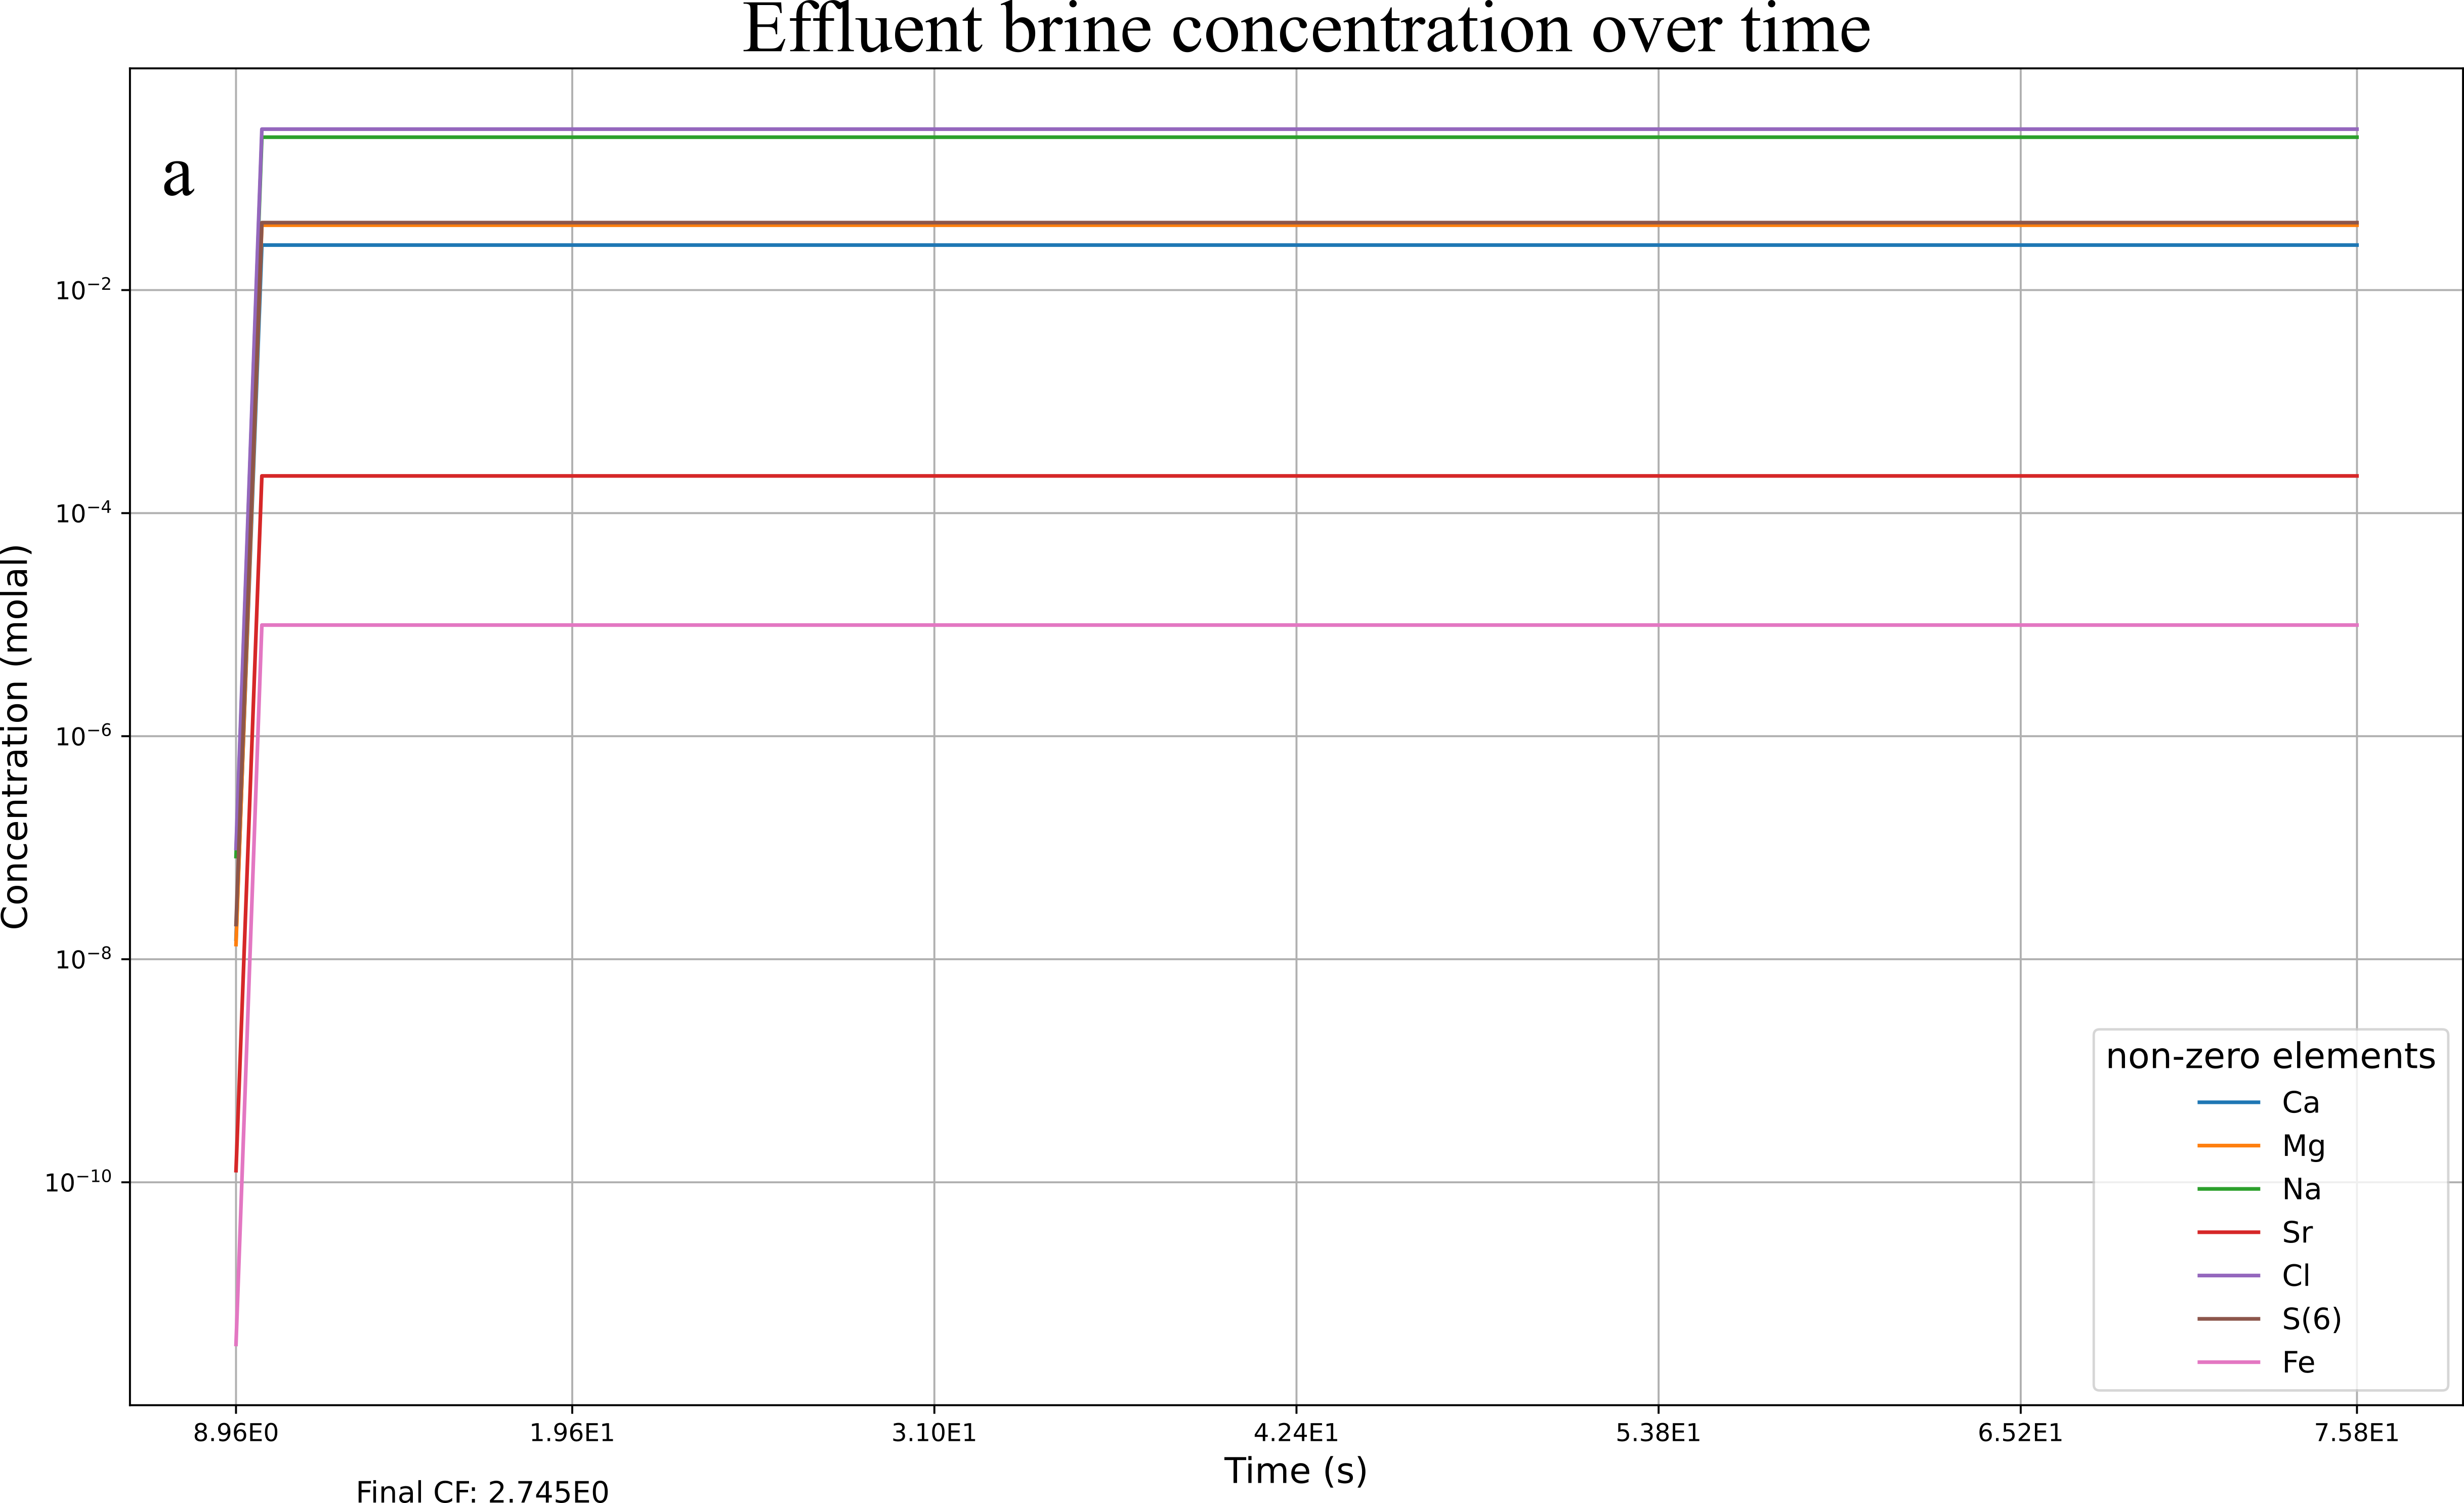
\includegraphics[width=0.8\linewidth]{images/ROSSpy/sensitivity_analyses/simulation_perspective/all_time_brine.png} \\ \midrule
        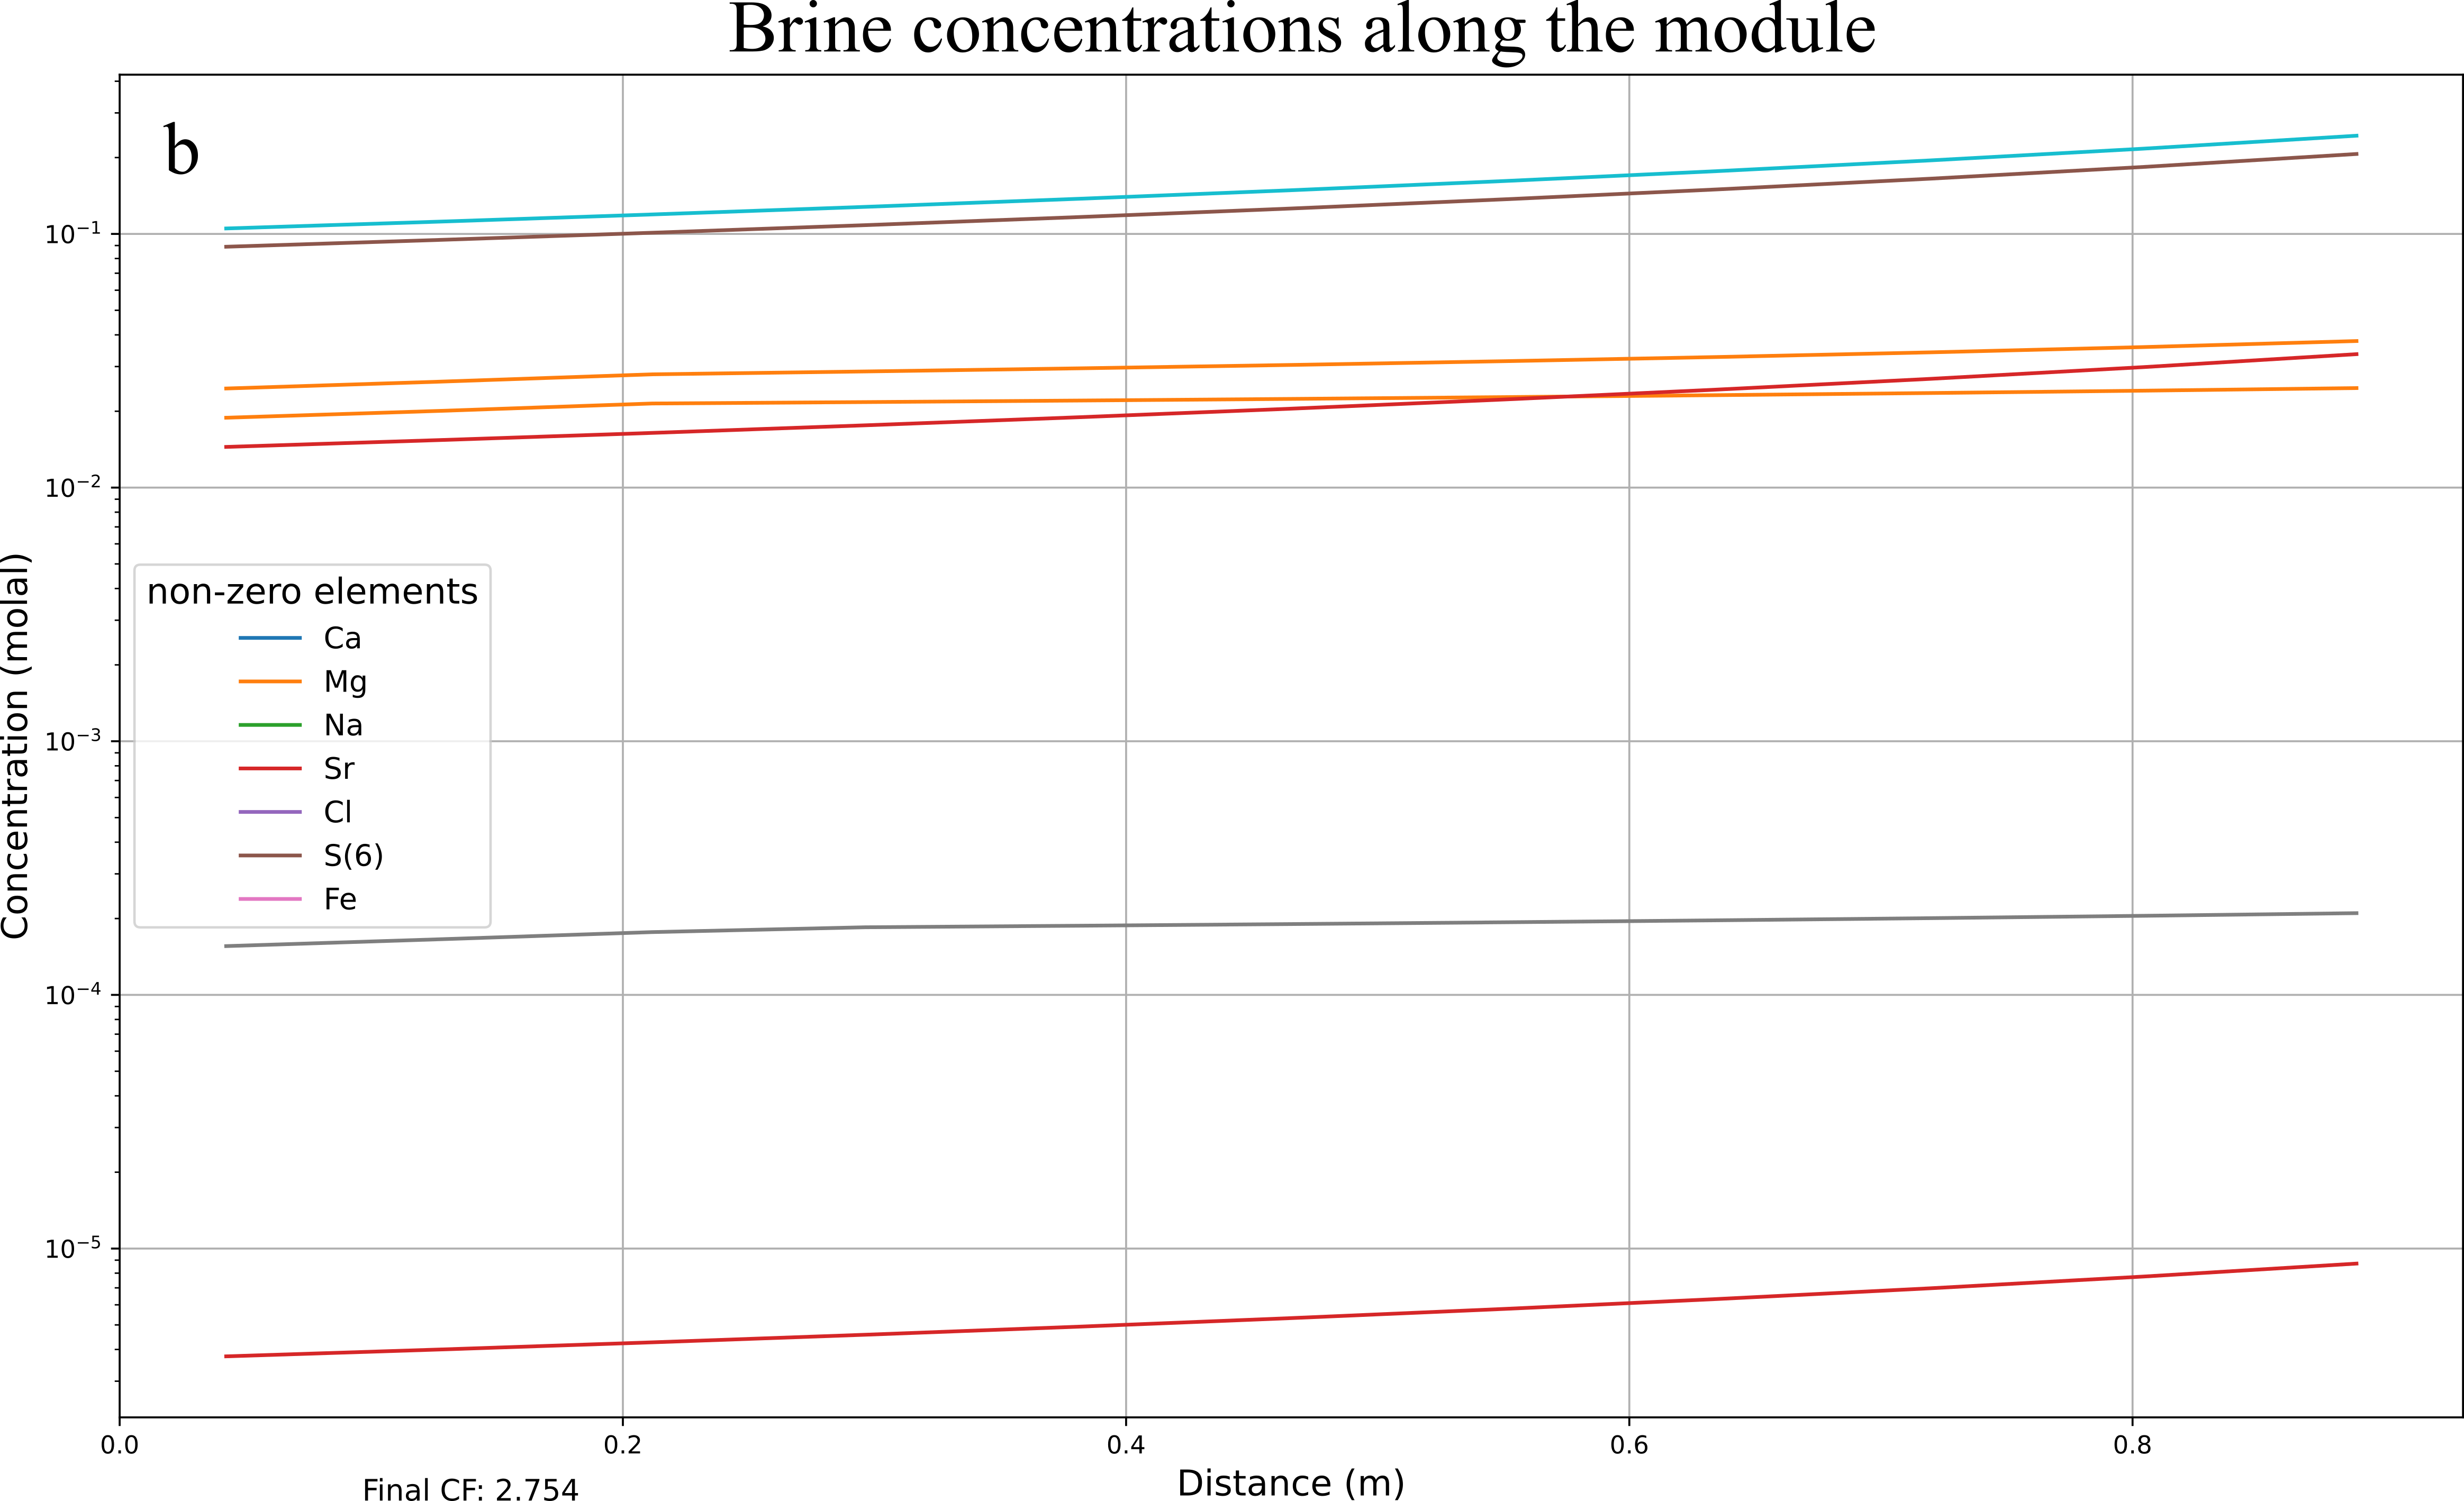
\includegraphics[width=0.8\linewidth]{images/ROSSpy/sensitivity_analyses/simulation_perspective/all_distance_brine.png}
    \end{tabular}
    \caption{
        Brine formation while slicing through either a) time at the final cell or b) distance at the final time. The end concentrations slightly differ between these two simulation perspectives, where the all\_time perspective calculates the true end of the last cell while the all\_distance perspective calculates the mid-point of the last cell and thus has a slightly lower concentration. The brine represents desalination of the Red Sea through the BW30-400 module.
    }
    \label{brine_perspectives}
\end{figure}

\begin{figure}
    \centering
    \begin{tabular}{c}
        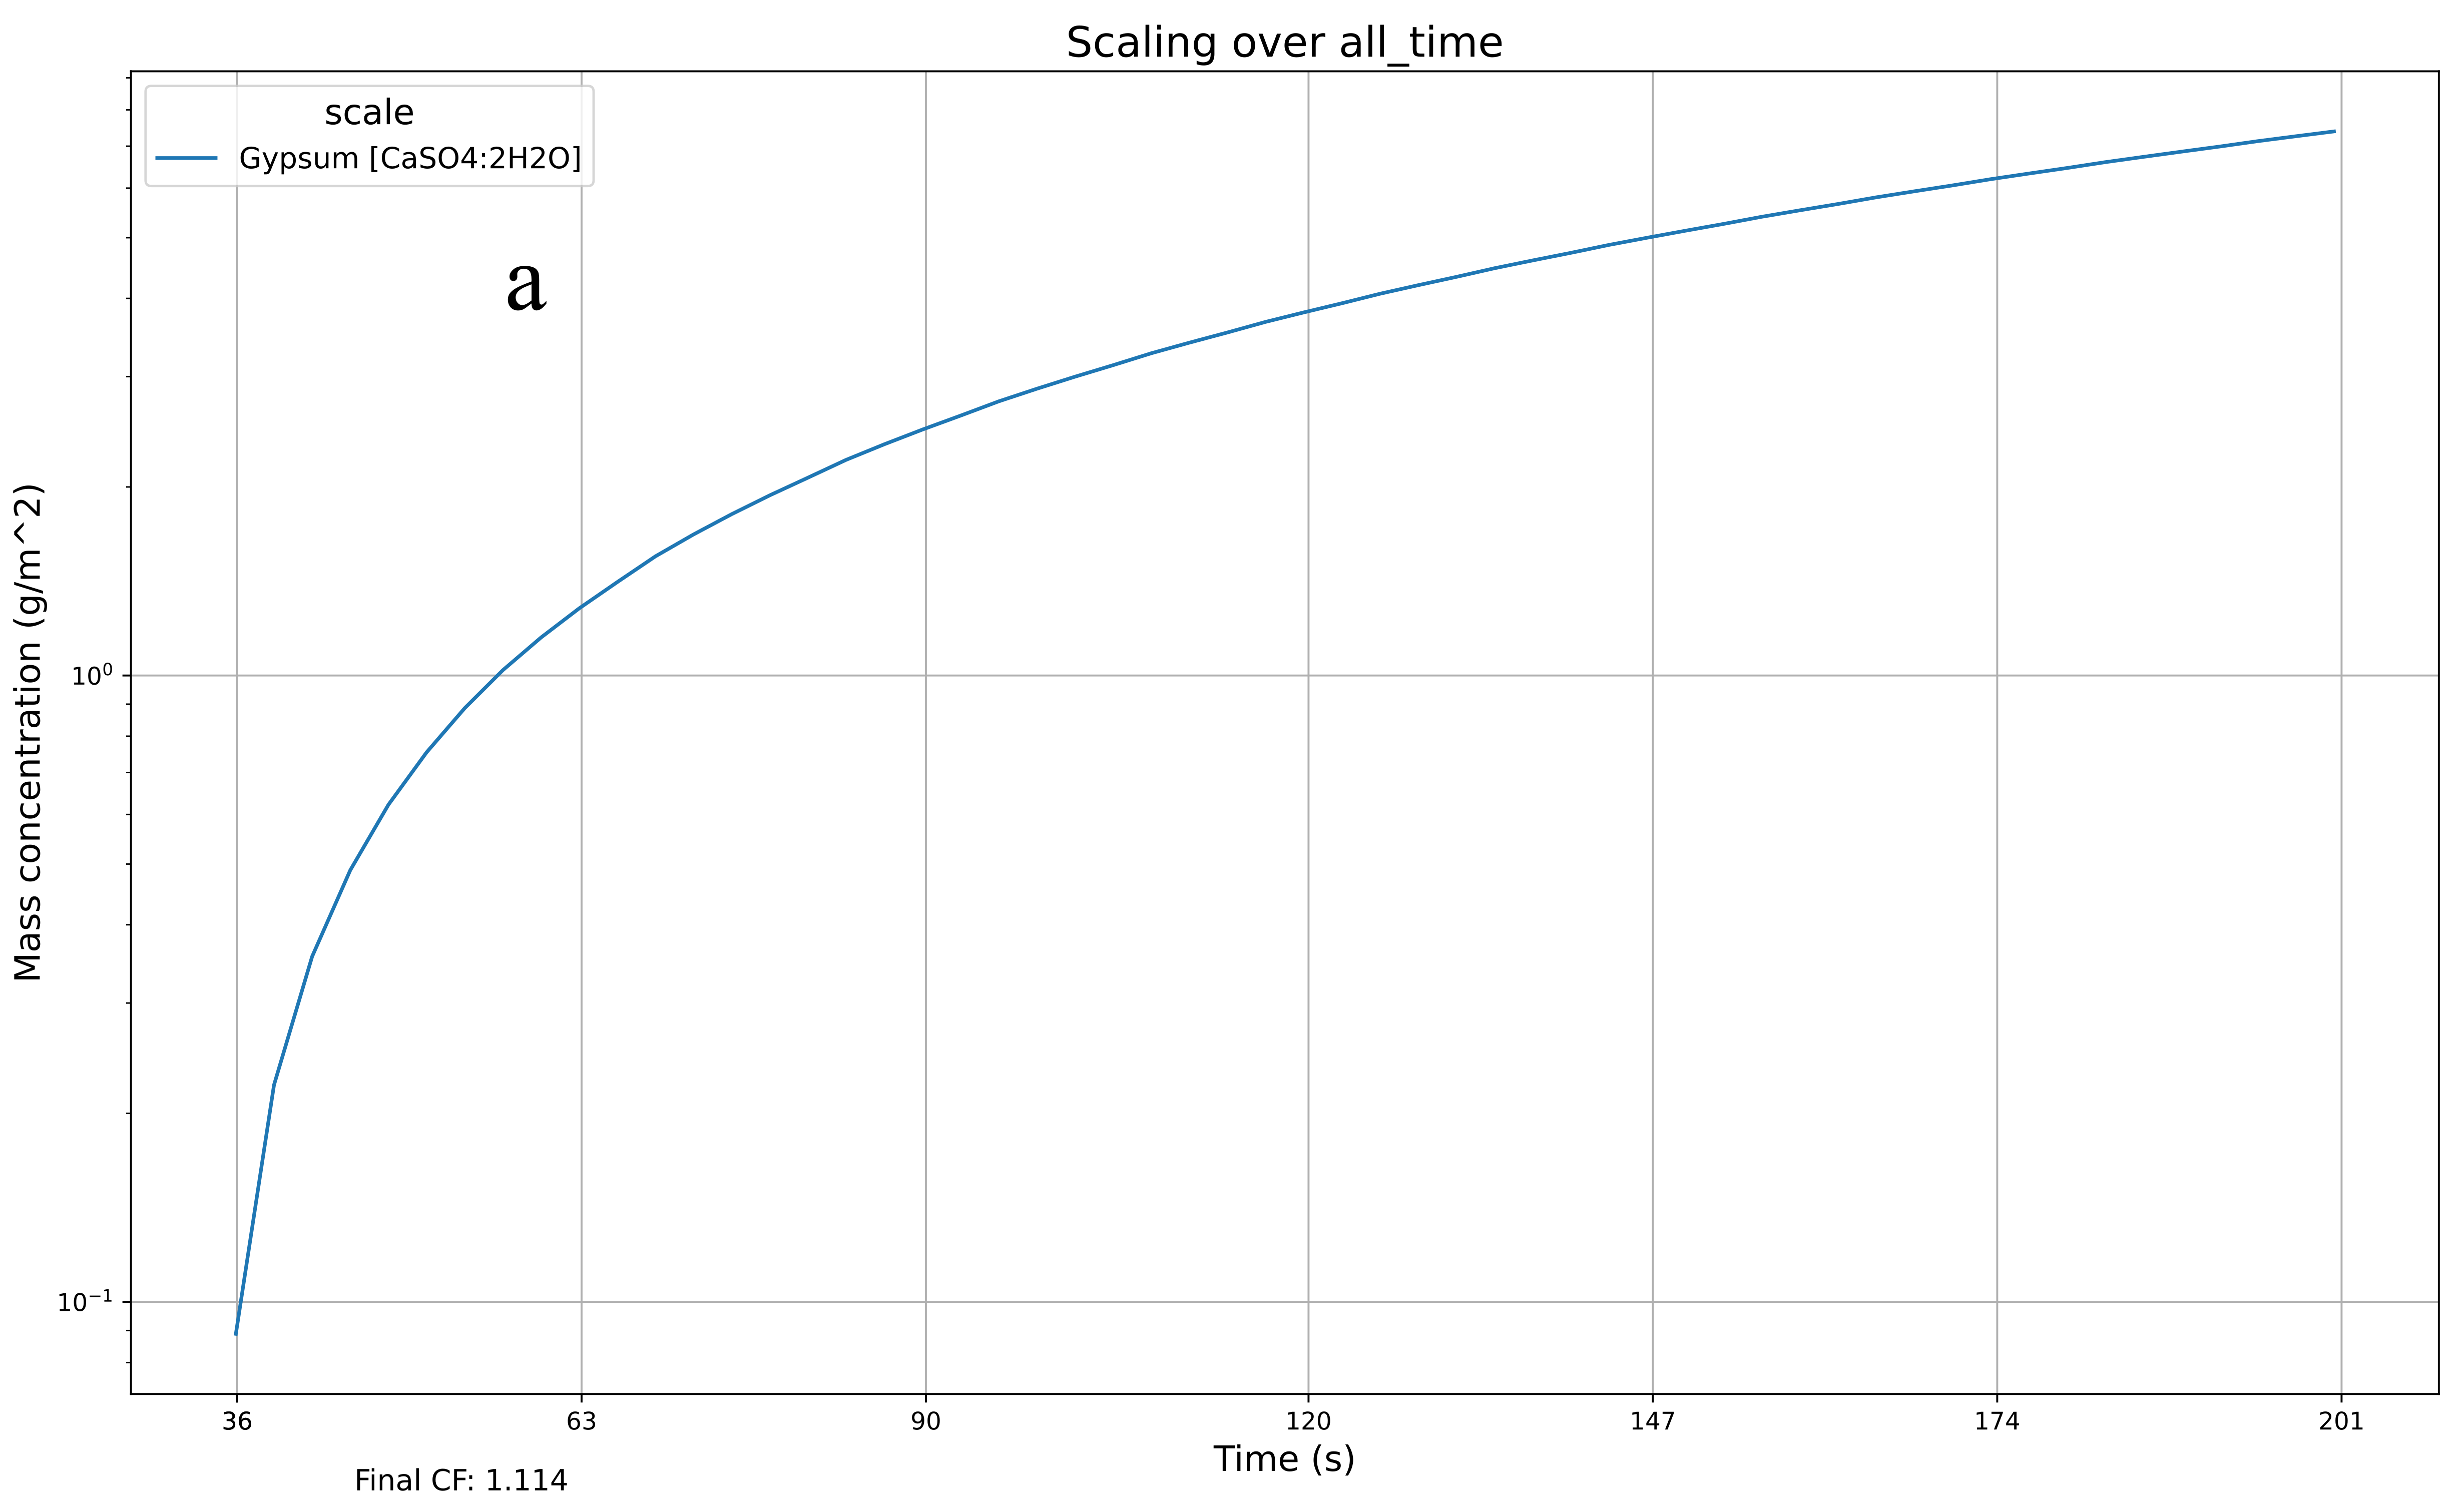
\includegraphics[width=\linewidth]{images/ROSSpy/sensitivity_analyses/simulation_perspective/all_time.png} 
        \\ \midrule
        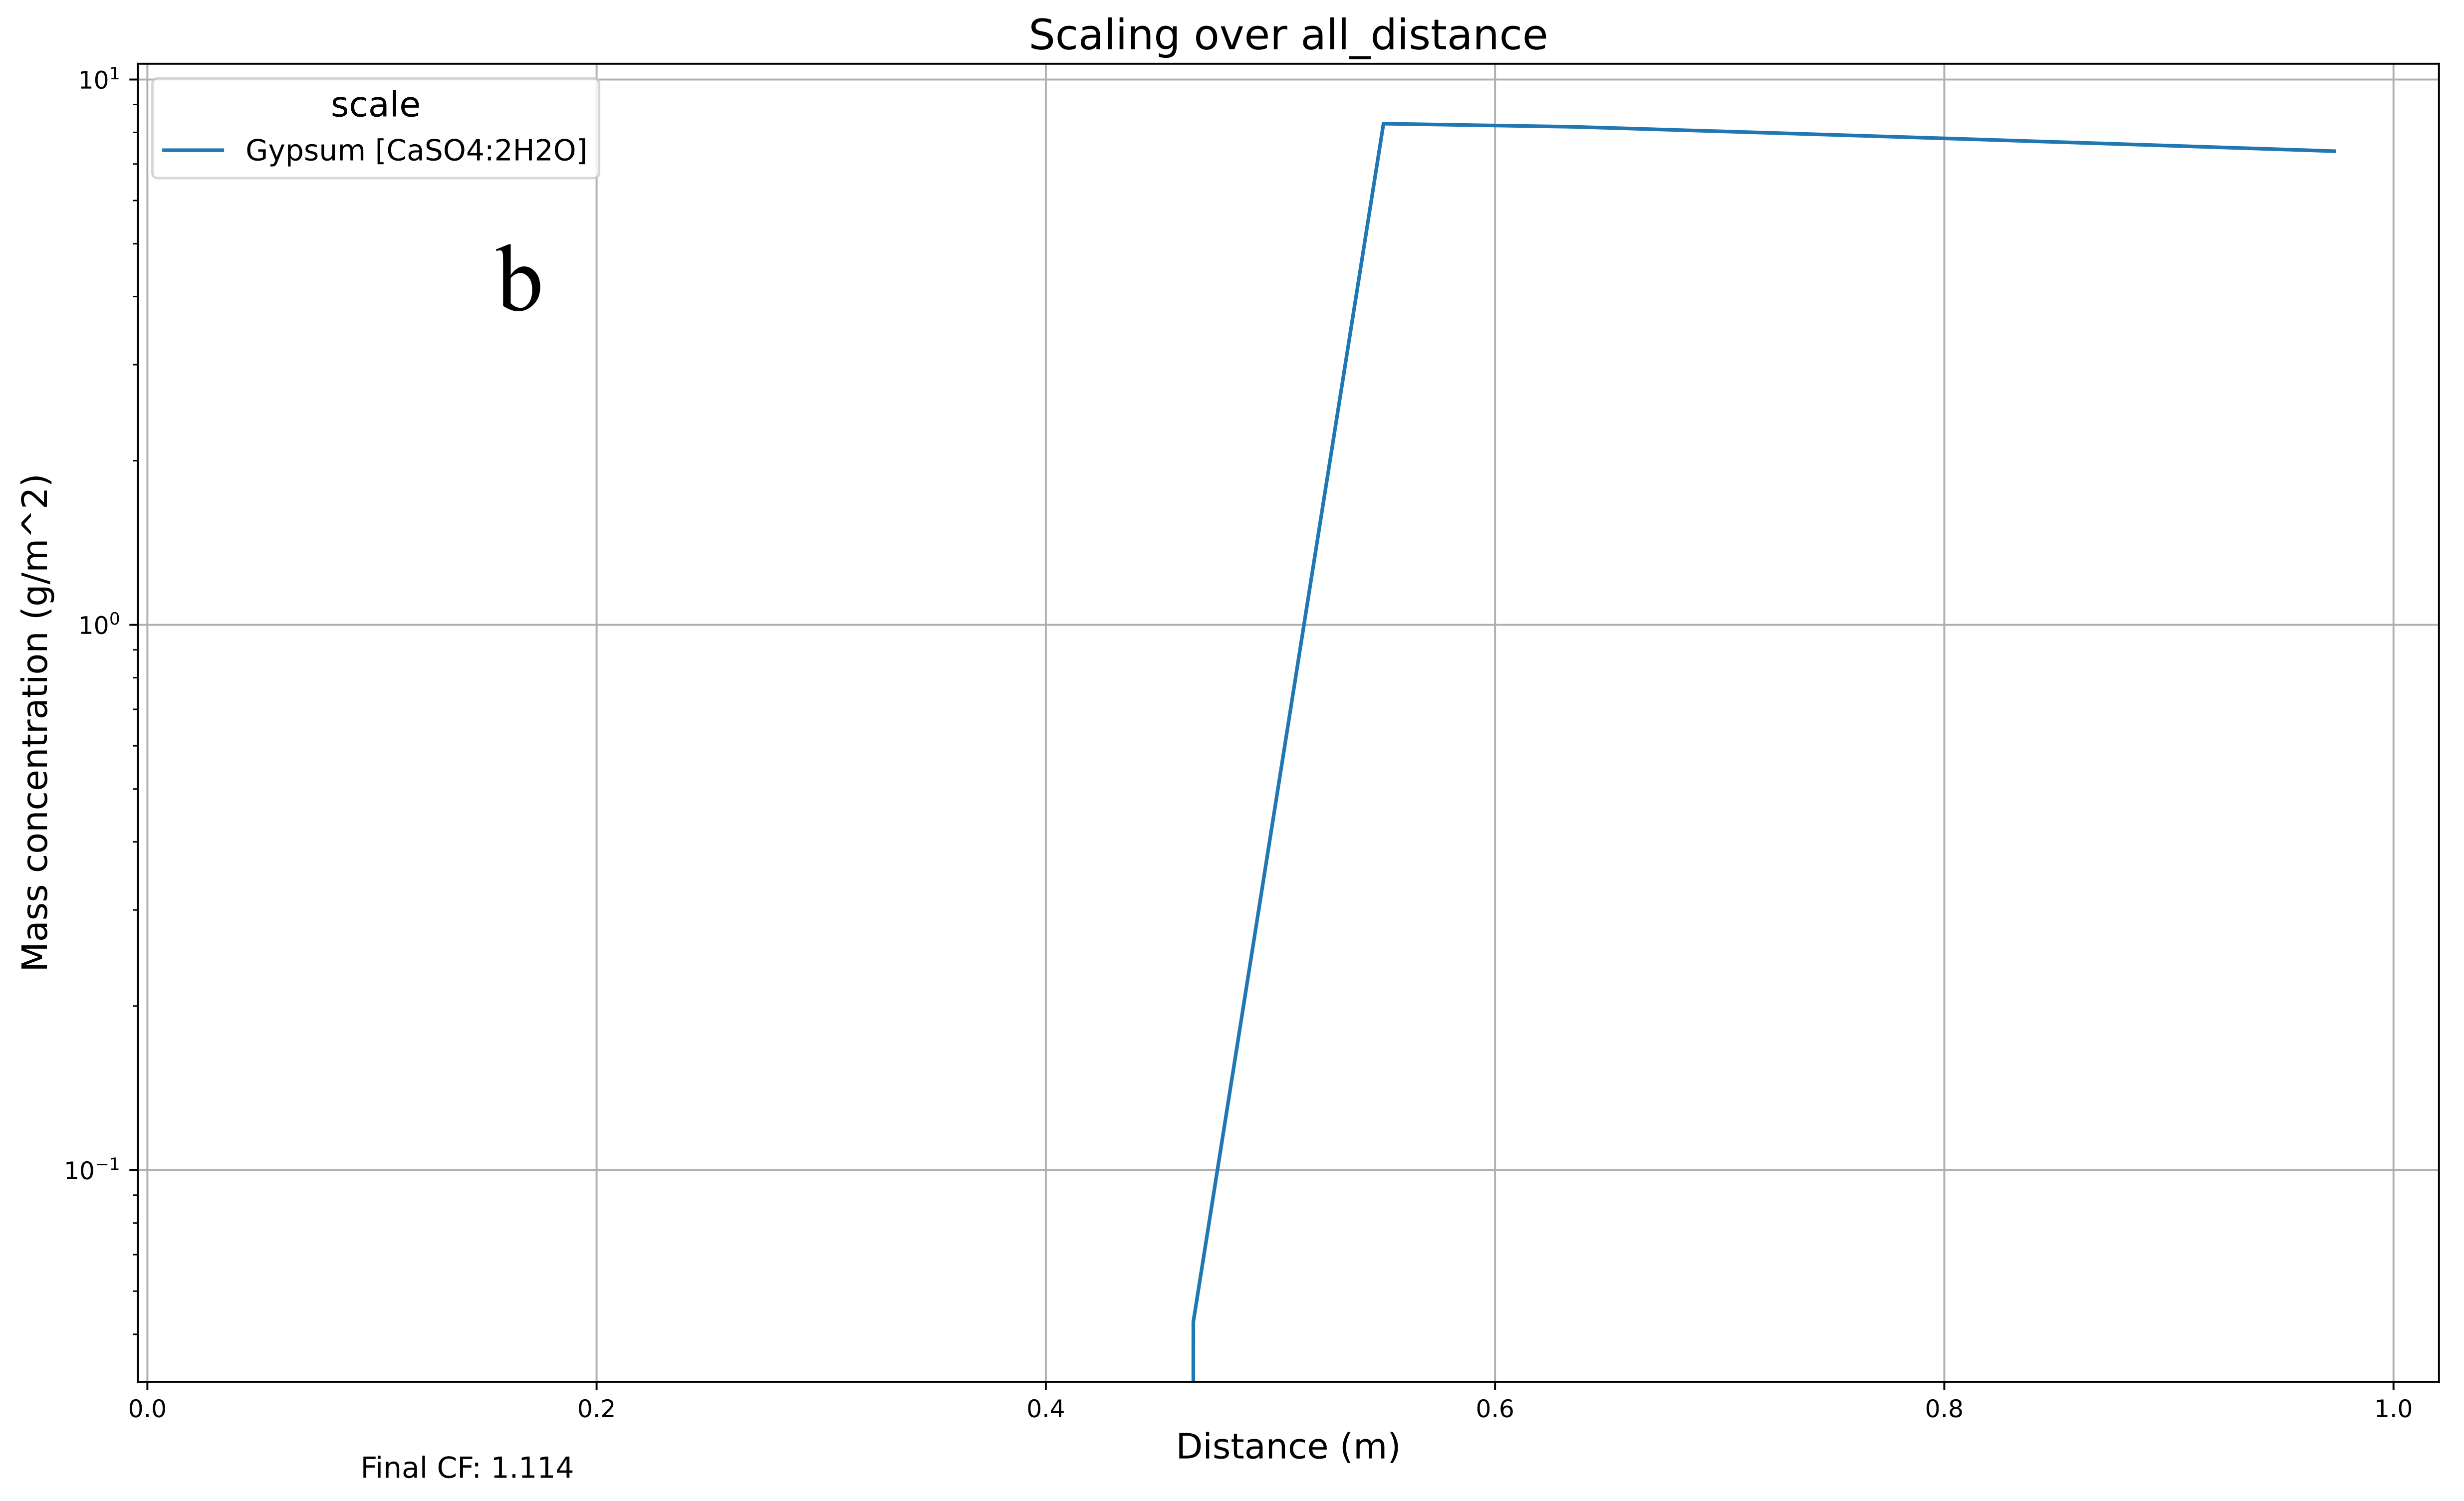
\includegraphics[width=\linewidth]{images/ROSSpy/sensitivity_analyses/simulation_perspective/all_distance.png} 
    \end{tabular}
    \caption{
        Scaling while either slicing through a) time at the final cell or b) distance at the final time. The underlying simulation was of the Red Sea through the BW30-400 module.
    }
    \label{scaling_perspectives}
\end{figure}

A cross-section of an RO module, which highlights boundaries of the single- and dual-domain solution models, is depicted in Figures \ref{single_dual_domain}.

\subsection{Software}

\subsection{PHREEQC consistency}

\subsubsection{ICE table calculations}
The expected precipitation in the presented ICE table of Table \ref{ice_table} was determined as $x$ in the following derivation:

\begin{equation} \label{ice_calculations}
    \begin{split}
        K_{sp} &= [a_{Ca^{2+}} - x]^1 * [a_{SO_4^{2-}} - x]^1 \\ 
        K_{sp} &= (\gamma*[Ca^{2+}] - x) * (\gamma*[SO_4^{2-}] - x) \\ 
        10^{-4.58} &= ((0.19*0.020594) - x) * ((0.06*0.105462) - x) \\ 
        10^{-4.58} &= (0.003913 - x) * (0.00633 - x) \\
        10^{-4.58} &= 2.477E-5 - 0.01024 + X^2 \\
        0 &= -1.54E-6 - 0.01022x + x^2 \\
         \therefore ~~ x &= 0.0104~molal = \frac{\fbox{0.181~moles}}{17.67~kg~water}~~.
    \end{split}
\end{equation}

The activity coefficients ($\gamma$) for $Ca^{2+}$ and $SO_4^{2-}$ were sourced from PHREEQC for this specific solution system. The $17.67~kg$ mass of water corresponds to the mass maximum capacity of the simulated BW30-400 module.  

The predicted precipitation in the presented ICE table of Table 1b ($gypsum\_pore\_volume$) are similarly derived:
\begin{equation} \label{PHREEQC_output_precipitation}
    \begin{split}
        gypsum\_pore\_volume &= gypsum\_all\_shifts * \frac{cells\_per\_module}{total\_simulation\_shifts} \\
         &= \sum_{i=1}^n (Gypsum_i) * \frac{12}{51} \\ 
         &= 0.823 * \frac{12}{51} \\ 
         &= 0.194 ~moles ~~.
    \end{split}
\end{equation}
The $\frac{12}{51}$ is the fraction of simulation shifts that correspond to a single module or pore volume, where the simulated module was discritized into $12$ cells. This isolates scaling from a single module, instead of the accumulation of scaling from multiple pore volumes, which renders the quantity directly comparable with the expected quantity.

\begin{table}[h]
    \centering
    \begin{tabular}{c|ccccc}
      \toprule
       & $Ca^{2+}$ & $+$ & $SO_4^{2-}$ & $\leftrightharpoons$ & $CaSO_4$ \\
      \midrule
      I & $0.003913$ && $0.00633$ && $0$ \\
      C & $-x$ && $-x$ && $+x$ \\
      F & $0.003913-x$ && $0.00633-x$ && $x$ \\
      \bottomrule
    \end{tabular}
    \caption{
        Gypsum precipitation according to the ICE (Initial, Change, Equilibrium) framework, except that "Equilibrium" (E) is replaced with "Final" (F) since the system does not reach equilibrium while within the module. The estimated Gypsum precipitation from a solution of $Ca^{2+}$ \& $SO_4^{2-}$ -- based upon the $K_{sp}$ of Gypsum and the activity coefficients of this solution from iPHREEQC -- is derived in \ref{ice_calculations} for the system in this table. 
        }
    \label{ice_table}
\end{table}

\subsubsection{Evaporation versus transport desalination}

The mechanism of concentrating a solution, either via evaporation or desalination, should not alter scaling predictions, ceterius paribus. Figure \ref{evaporation} contrasts scaling predictions from evaporation and desalination of the Red Sea, where the two mechanisms are approximately equivalent. Differences are postulated to originate from the consideration of advection in the latter but not the former.

\begin{figure}
    \centering
    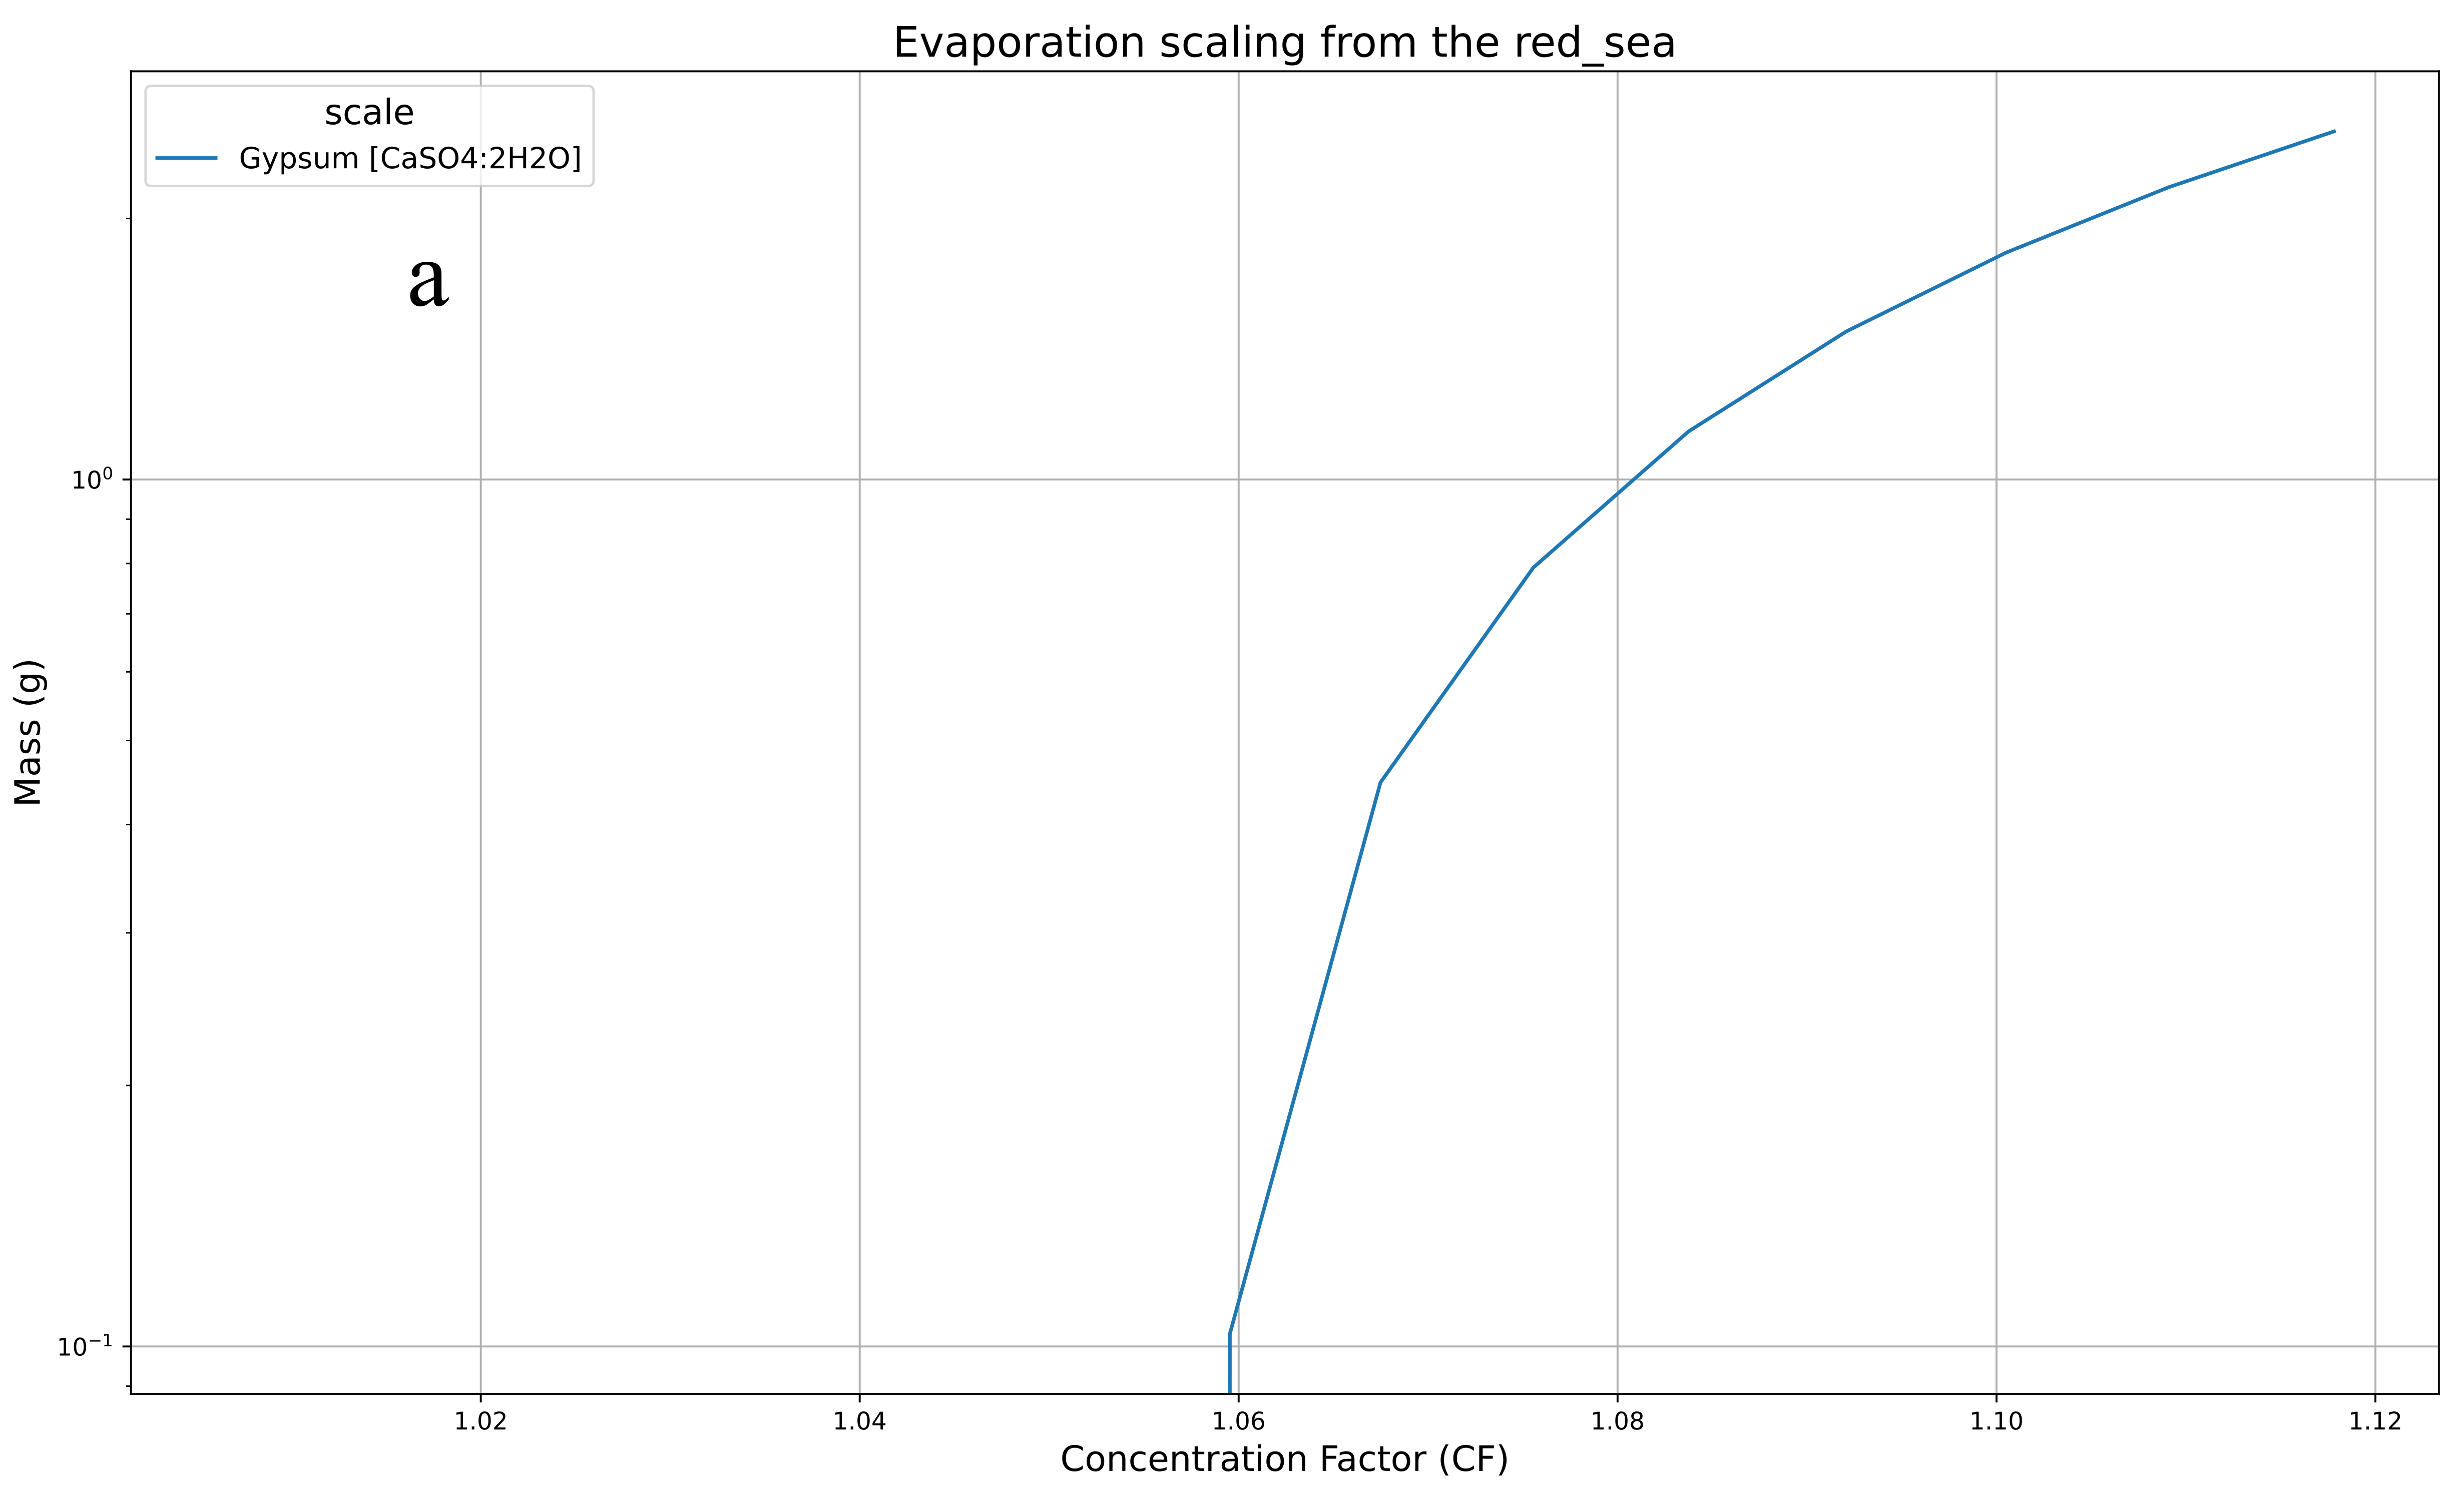
\includegraphics[width=\linewidth]{images/ROSSpy/sensitivity_analyses/evaporation/evaporation.png} \\ \midrule
    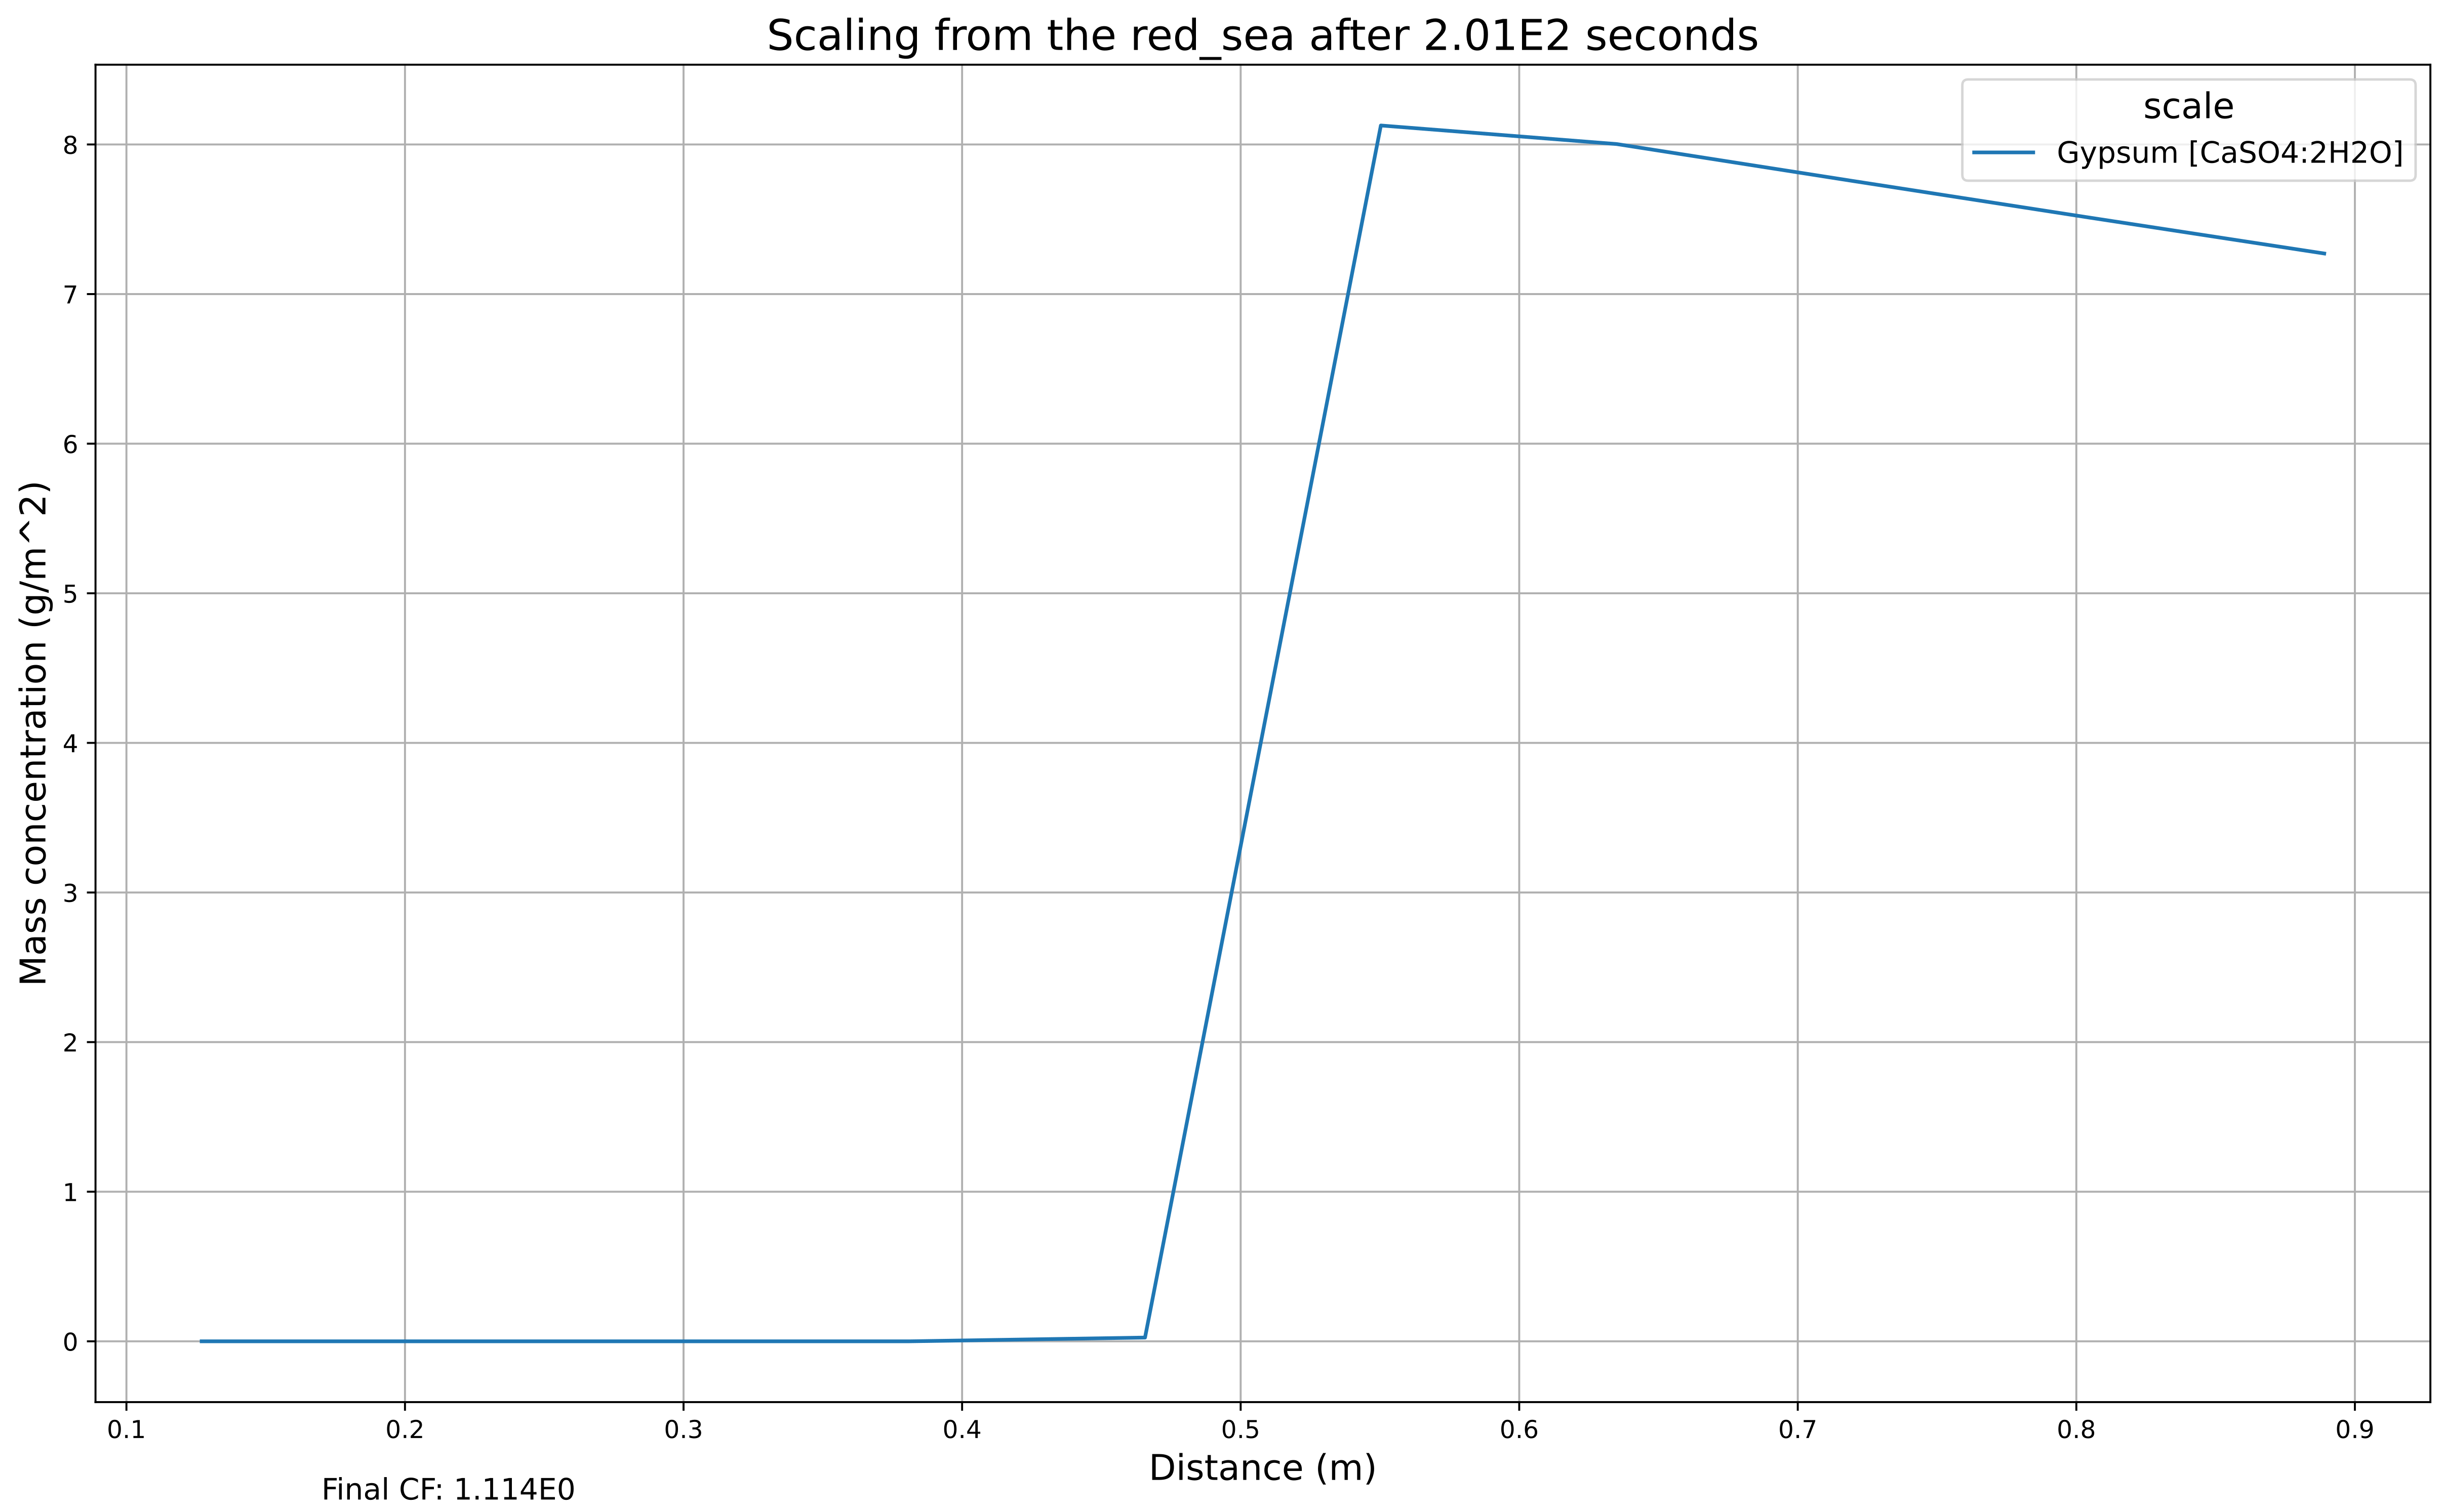
\includegraphics[width=\linewidth]{images/ROSSpy/sensitivity_analyses/evaporation/desalination.png}
    \caption{
        Scaling while a) evaporating and b) desalinating the Red Sea. The two scaling predictions are qualitatively similar, however, even after accounting for the accumulation amongst different pore volumes, the evaporation predictions ($3.36g$) are less than those of the reaction transport simulation ($5.27g$). The difference may be the absence of advection in the evaporation analysis.
    }
    \label{evaporation}
\end{figure}


\subsection{In-series RO arrangements}

In-series arrangements of multiple RO modules are represented by compounding individual modules. We determined that this approach is preferential to a few other methods: e.g. amplifying the characteristics of a single RO module, such as those in Table \ref{RO_dimensions}, by a scalar $r=\frac{\Phi_{\Delta multi-module}}{\Phi_{\Delta module}}$, where the $\Delta \Phi_{multi-module}$ is the total permeate flux of the multi-module system that can be parameterized or approximated through eq. (8). The substitution of $CF_{multi}$ for $CF_e$ and $\Delta \Phi_{multi-module}$ for $\Phi_e$ into eq. (9) permits calculating the $\Delta \Phi_{multi-module}$. 

\begin{savenotes}
\begin{table}[!h]
    \centering
    \begin{tabular}{|c|c|c|}
        \toprule
        \textbf{Parameter} & \textbf{Value} & \textbf{Source} \\ \midrule
        
        \multicolumn{3}{c}{Module (m)} \\ \midrule
        length & 1.016 & BW30-400 \cite{2020FilmTecElement} \\ 
        diameter & 0.201 & BW30-400 \cite{2020FilmTecElement}\\
        permeate tube diameter & 0.029 & BW30-400 \cite{2020FilmTecElement}\\ \midrule
        
        \multicolumn{3}{c}{Membrane (mm)} \\ \midrule
        filtration layer & 0.00025 & \cite{Pacheco2010CharacterizationTechniques,Jeong2007InterfacialMembranes} \\
        Feed spacer & 0.8636 & BW30-400 \cite{2020FilmTecElement} \& \cite{Sablani2002InfluenceSystems} \\
        Permeate spacer & 0.3 & \\
        Polysulphonic layer & 0.05 &  \\
        Support layer & 0.15 &  \\
        Windings $\left( \frac{th_{total}}{th_{membrane}} \right) $ & 86 & BW30-400 \cite{2020FilmTecElement} \\ \midrule
        
        \multicolumn{3}{c}{Membrane cross-section ($m^2$)} \\ \midrule
        Module & 0.0317 & BW30-400 \cite{2020FilmTecElement}\\
        Permeate tube & 0.000661 & BW30-400 \cite{2020FilmTecElement}\\
        Filtration section & 0.0311 & BW30-400 \cite{2020FilmTecElement}\\
        Feed channel & 0.0157 & BW30-400 \cite{2020FilmTecElement}\\ \midrule
        
        \multicolumn{3}{c}{Feed channel capacity} \\ \midrule
        Volume ($m^3$) & 0.0159 & BW30-400 \cite{2020FilmTecElement}\\
        Mass (kg) & 15.86 & BW30-400 \cite{2020FilmTecElement}\\ \midrule

        \multicolumn{3}{c}{Fluid flow ($\frac{m^3}{second}$)} \\ \midrule
        Permeate & 0.000463 & BW30-400 \cite{2020FilmTecElement}\\
        Max Feed & 0.00442 & BW30-400 \cite{2020FilmTecElement}\\ \bottomrule
        
    \end{tabular}
    \caption{
        Default dimensions of an RO module, with corresponding citations, that are primarily based upon the DOW FILMTEC BW30-400 RO module, following precedence from other software \cite{Li2012OptimalDesalination}.
    }
    \label{RO_dimensions}
\end{table}
\end{savenotes}

\subsection{Water bodies}

Additional feed parameter files can be composed by emulating the structure of the default feed parameter files. Literature sources that may foster the development of such feed parameter files for numerous potential feed sources are provided in Table \ref{new_water_bodies} with the respective citations of the experimental geochemical data. 

\begin{table}[h!]
    \centering
    \begin{tabular}{|c|c|}
        \toprule
        \textbf{Water body} & \textbf{Geochemical measurements} \\
        \midrule
        Indian Ocean & \cite{Danielsson1980CadmiumWater,Nisha2014GeochemicalIndia,Stephen-Pichaimani2008EnrichmentIndia,Selvaraj2004EvaluationApproaches,Thangadurai2005Pre-tsunamiIndia,ParvezAl-Usmani2015TraceIndia,Sabine2002InorganicProcesses,Singh2013InternalBengal} \\
        Sargasso Sea & \cite{Bender1976DissolvedSea,Stoffyn-Egli1984MassOceans} \\
        South China Sea & \cite{Calvert1993GeochemistrySeas,Wen2006PhysicochemicalSea,Du2020DynamicsStudy,Chen2001NutrientBasin,Nakaguchi2004DissolvedSea} \\
        Greek Coast & \cite{Chester1981TheSediments,Voutsinou-Taliadouri1983DistributionGreece,Voutsinou-Taliadouri1997DissolvedSeawater} \\
        Toyko Bay & \cite{Fukushima1992TraceJapan} \\
        California Coast & \cite{Hershelman1981MetalsOutfall,Luoma1988DistributionBay,Biller2013SourcesSeason} \\
        North Atlantic & \cite{Loring1978GeochemistryLawrence.,Loring1979GeochemistryLawrence,Yeats1983PotentialAtlantic,Bothner1998MetalTime,Campbell1980BaselineBay,Gaulier2019TraceWaters,Statham1986Dissolved0-35N,Mohamed2011DissolvedOcean,Guay1998ASeas} \\
        Baltic Sea & \cite{Szefer1995DistributionSea,Kremling1978TheStation} \\
        North Pacific & \cite{Tanita2015SurfacePacific,Sim2019Annual20102013} \\
        South Pacific & \cite{Boyle1975CopperZealand,Boyle1976OnCadmium} \\
        General natural waters & \cite{Alibo1999RareOxidation,Klinkhammer1983RareVents,Garcia-Solsona2020RareSea,Longinelli1967Oxygen-18Lakes,Llyod1967Oxygen-18Sulfate,Culkin1966SodiumWater,Krumgalz1982CalciumWaters} \\
        Mississippi Salt Dome Basin & \cite{Kharaka1987GeochemistryU.S.A.} \\
        \bottomrule
    \end{tabular}
    \caption{
        Proposed literature of potential feed water that can be adapted into parameter files for simulation in our model, or specifically ROSSpy.
    }
    \label{new_water_bodies}
\end{table}

\subsection{Dual domain}

\begin{figure}
    \centering
    \begin{tabular}{c|c}
        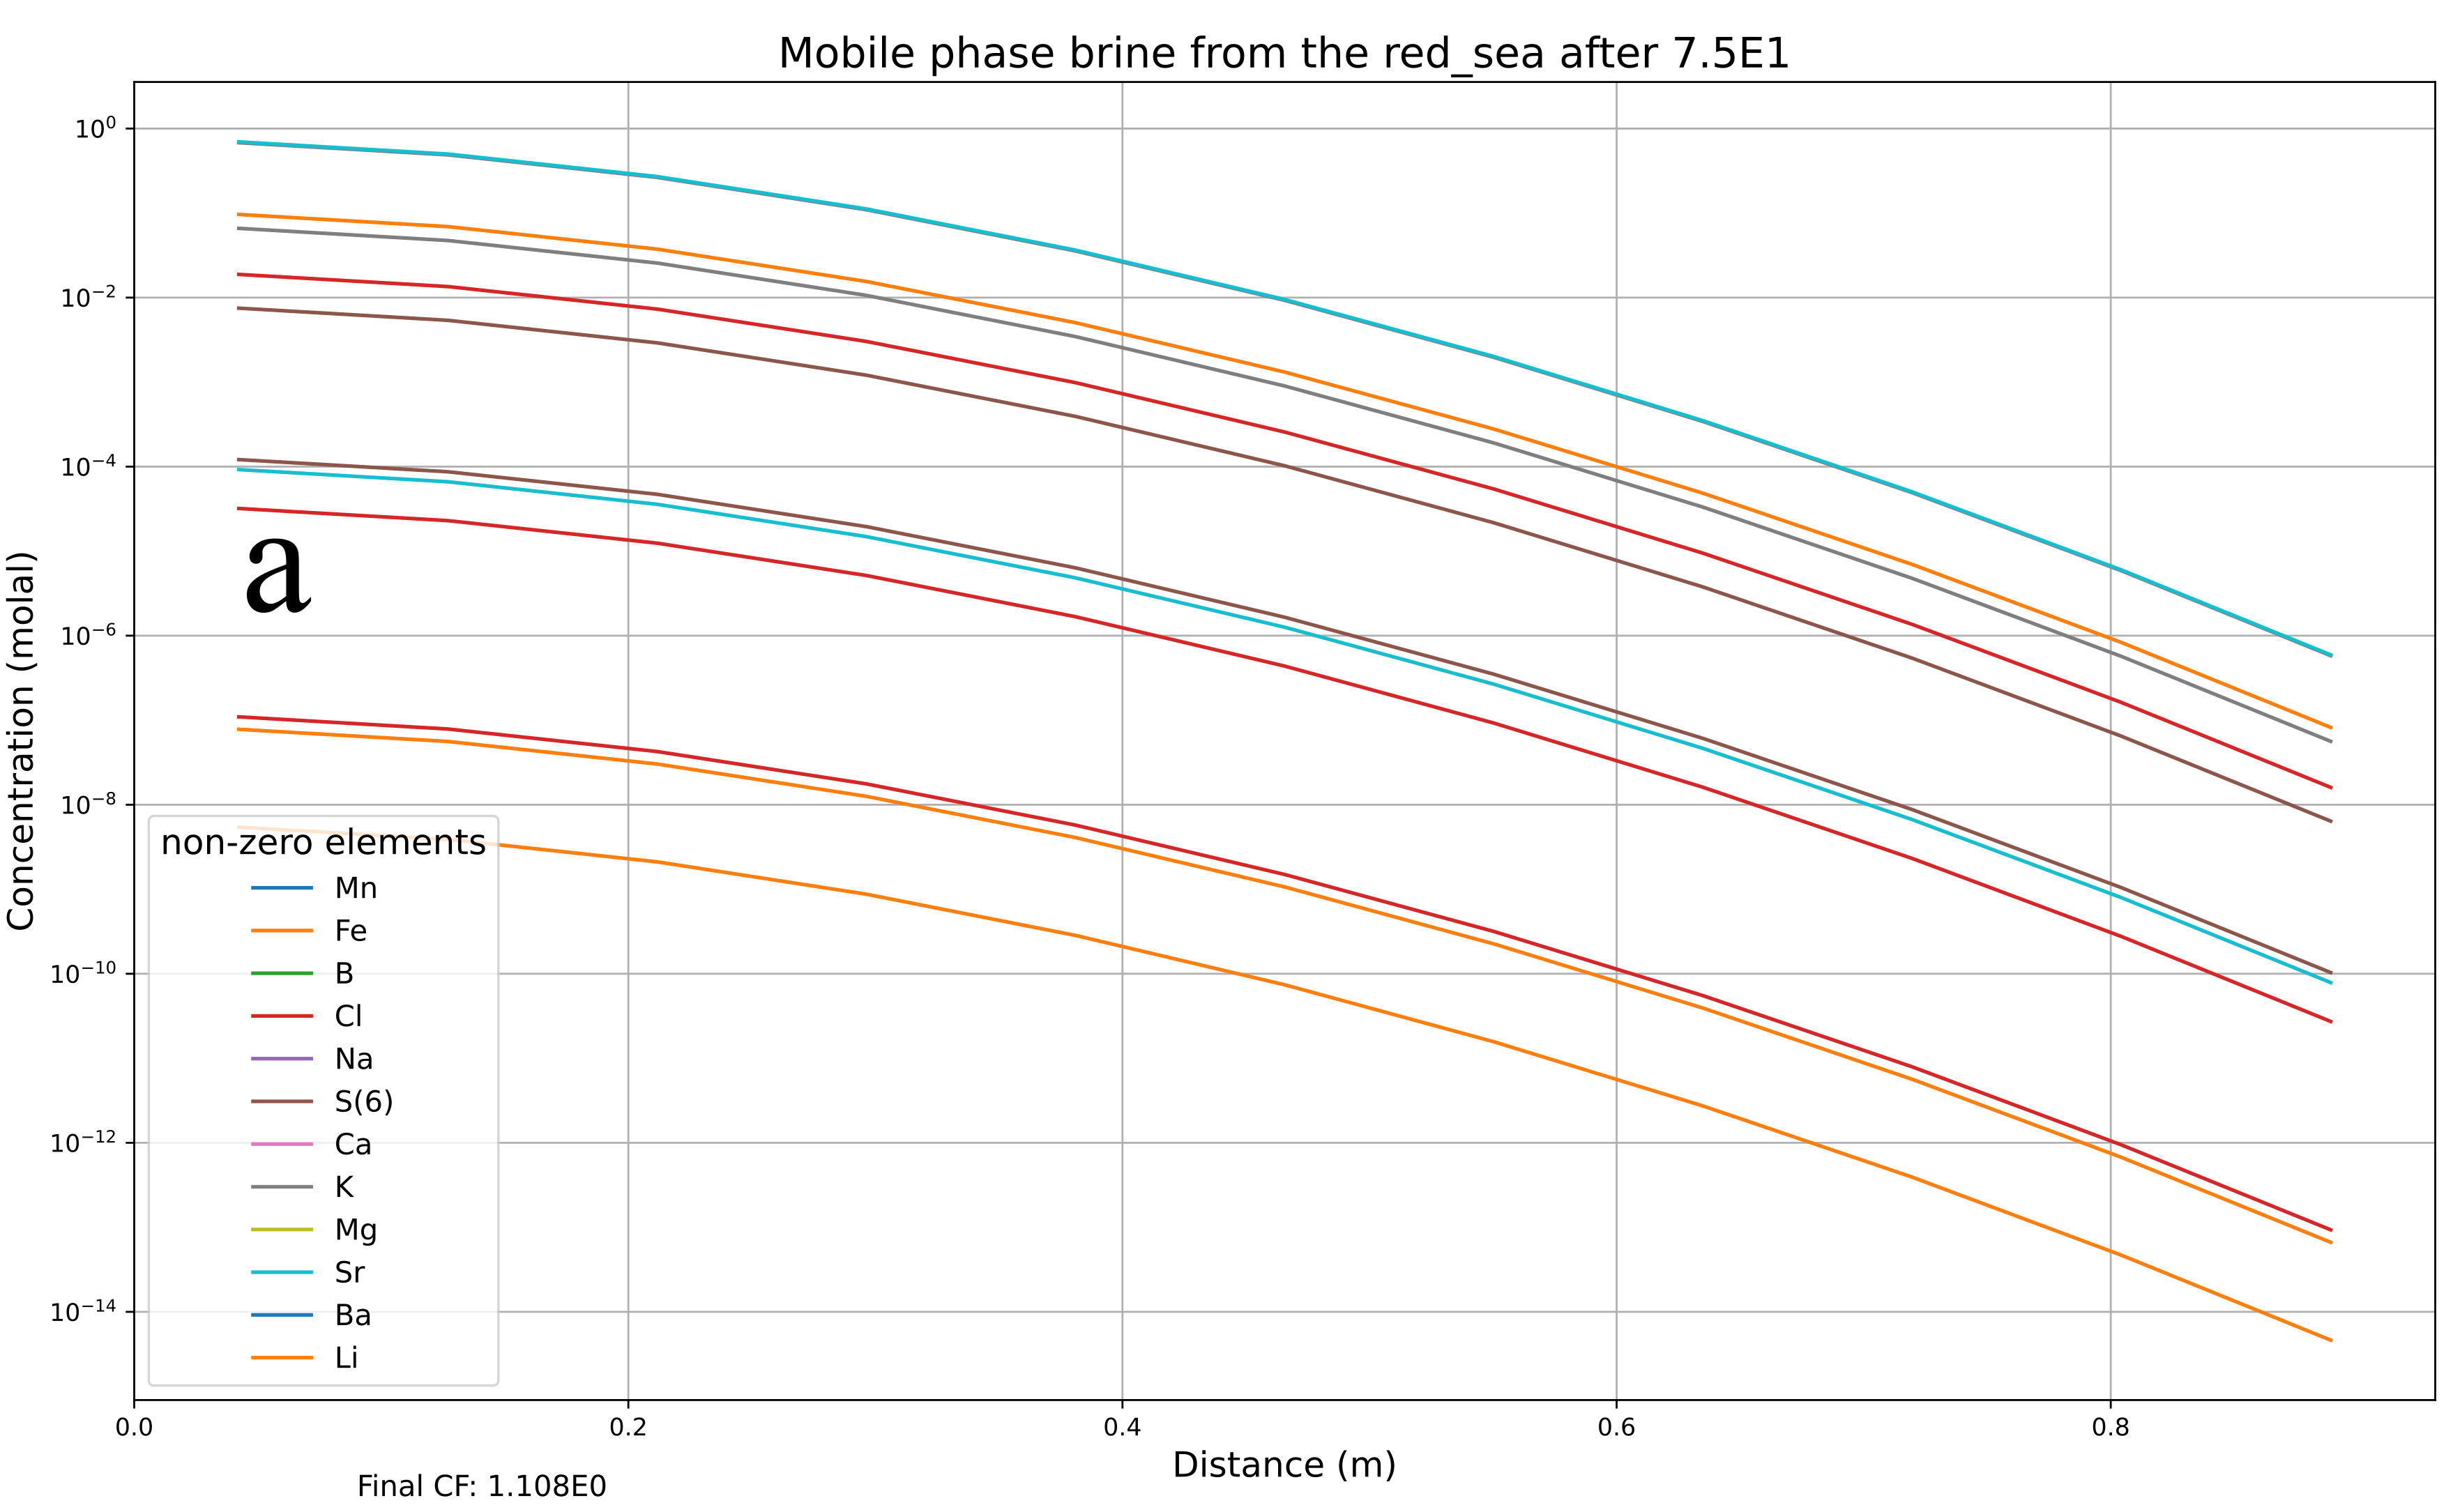
\includegraphics[width=0.49\textwidth]{images/ROSSpy/sensitivity_analyses/EF/mobile_large_ef.png} &
        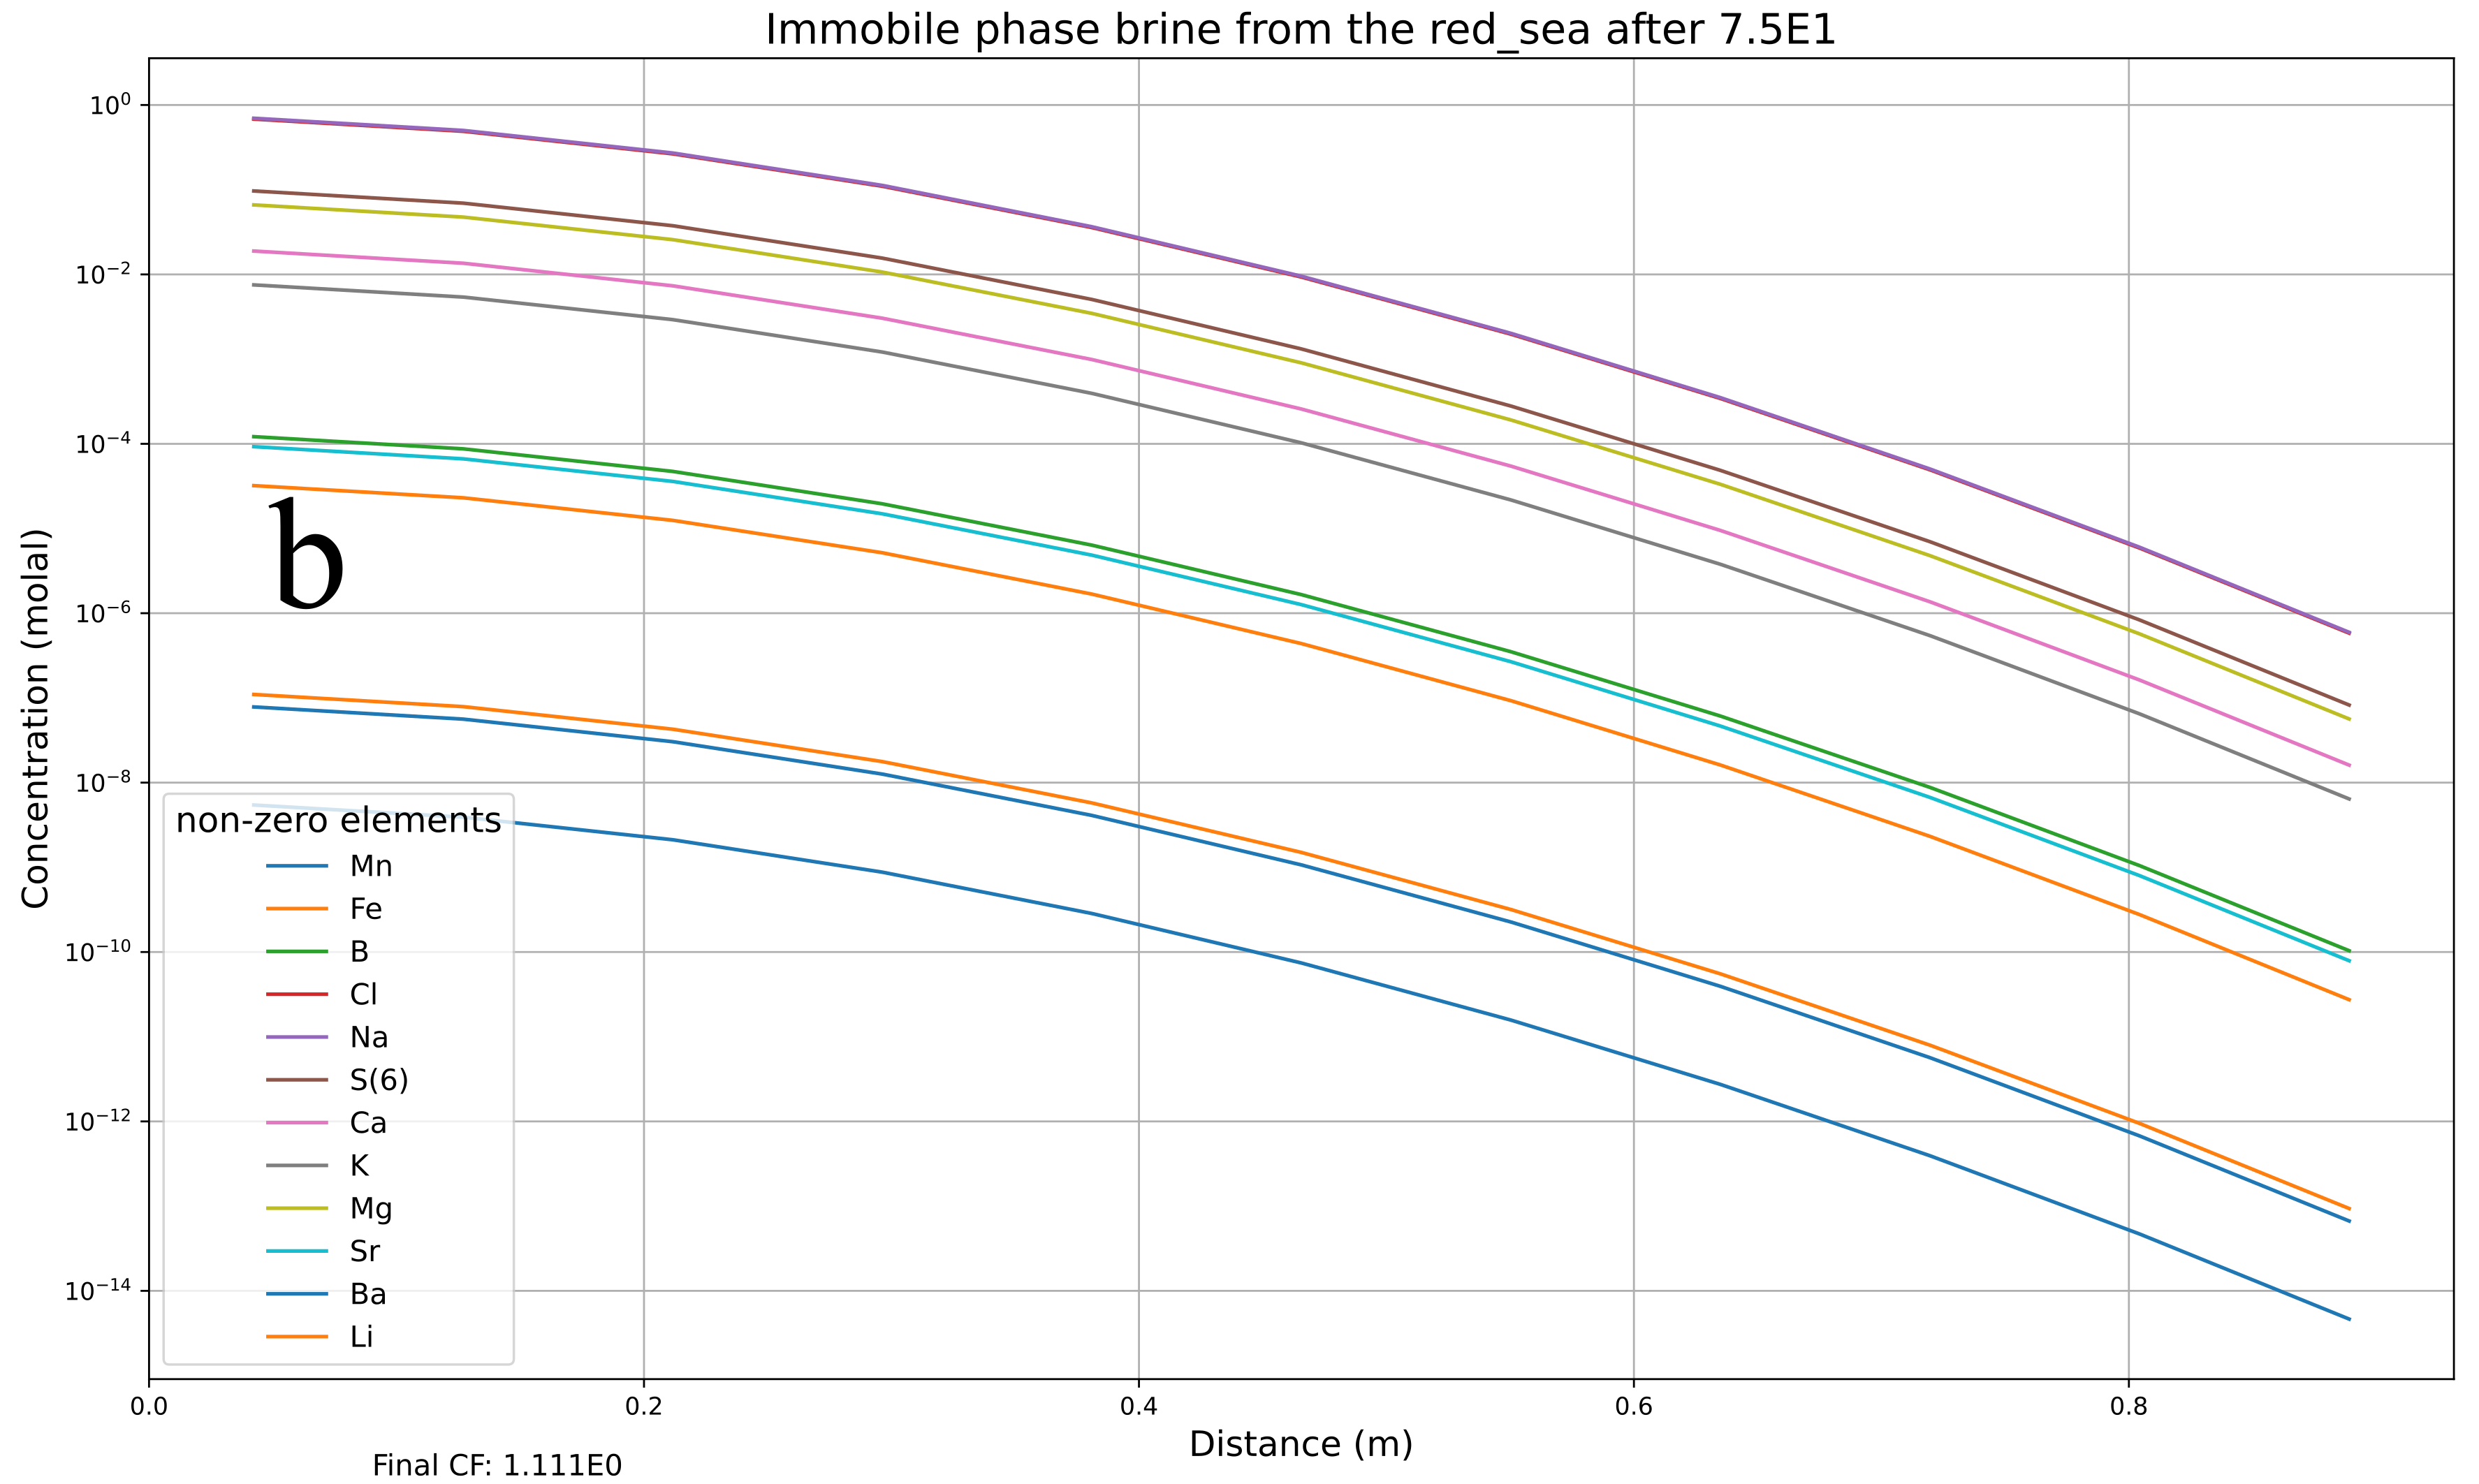
\includegraphics[width=0.49\textwidth]{images/ROSSpy/sensitivity_analyses/EF/immobile_large_ef.png} \\ \midrule
        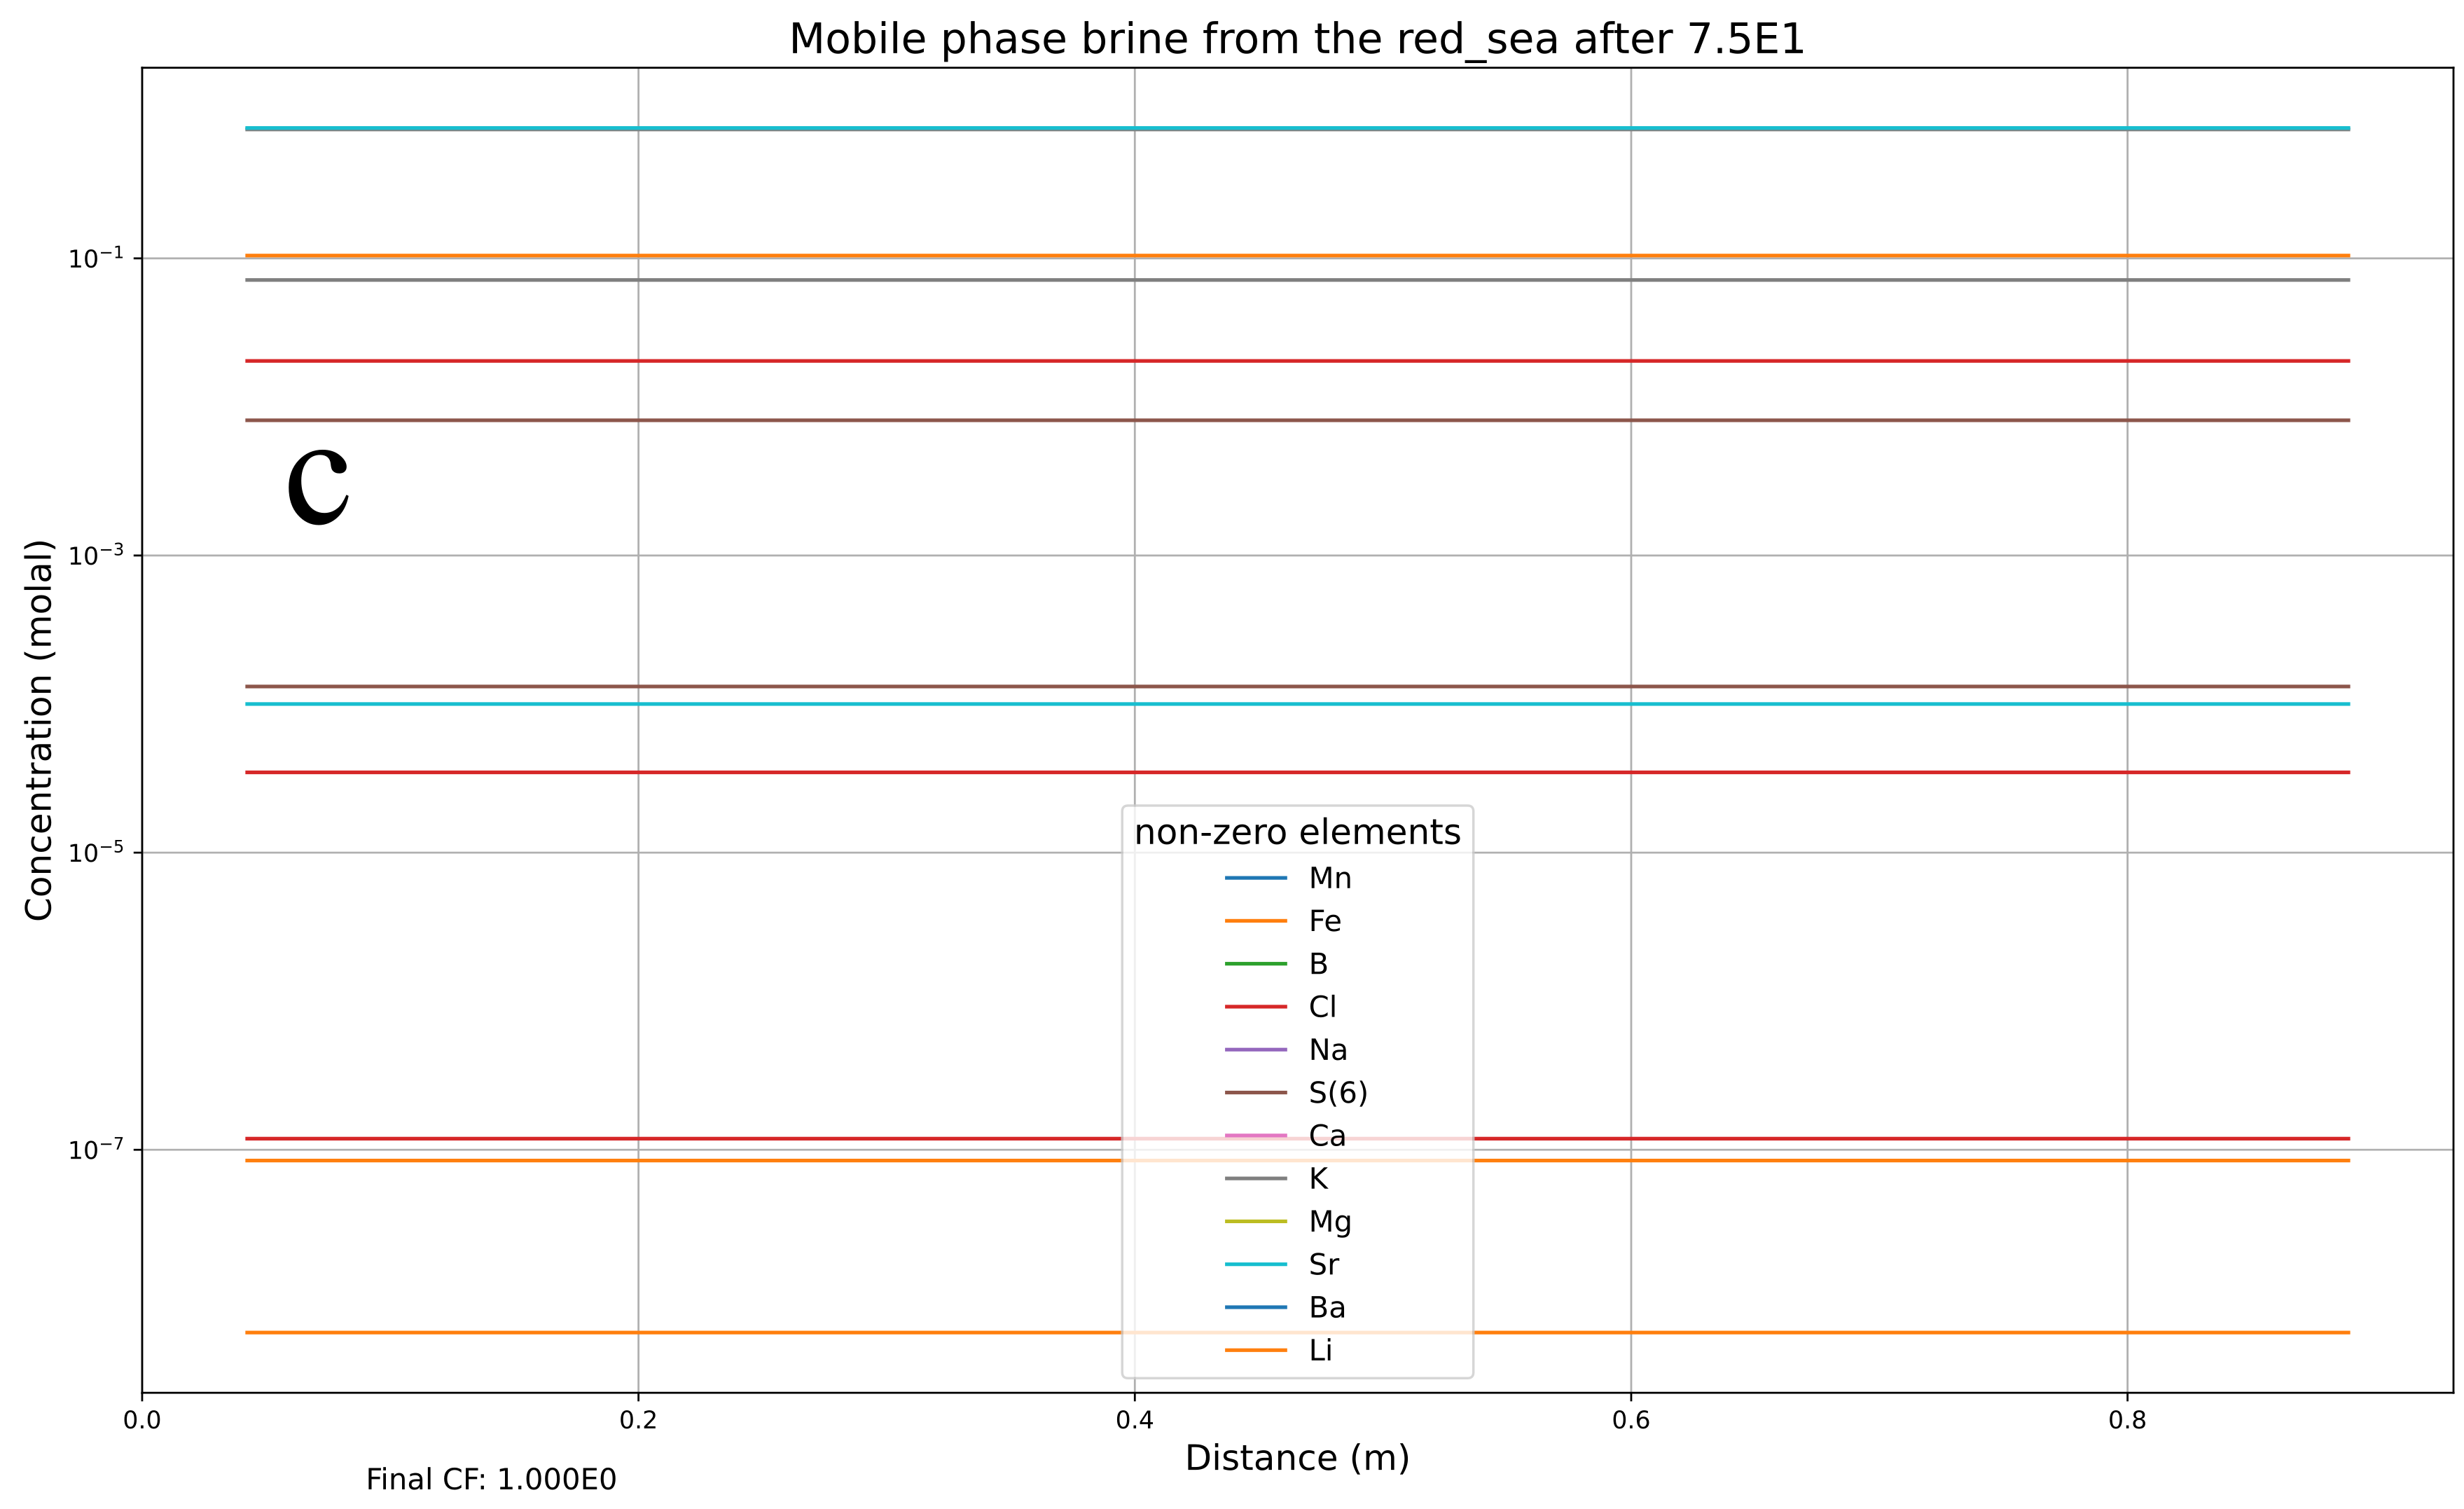
\includegraphics[width=0.49\textwidth]{images/ROSSpy/sensitivity_analyses/EF/mobile_small_ef.png} & 
        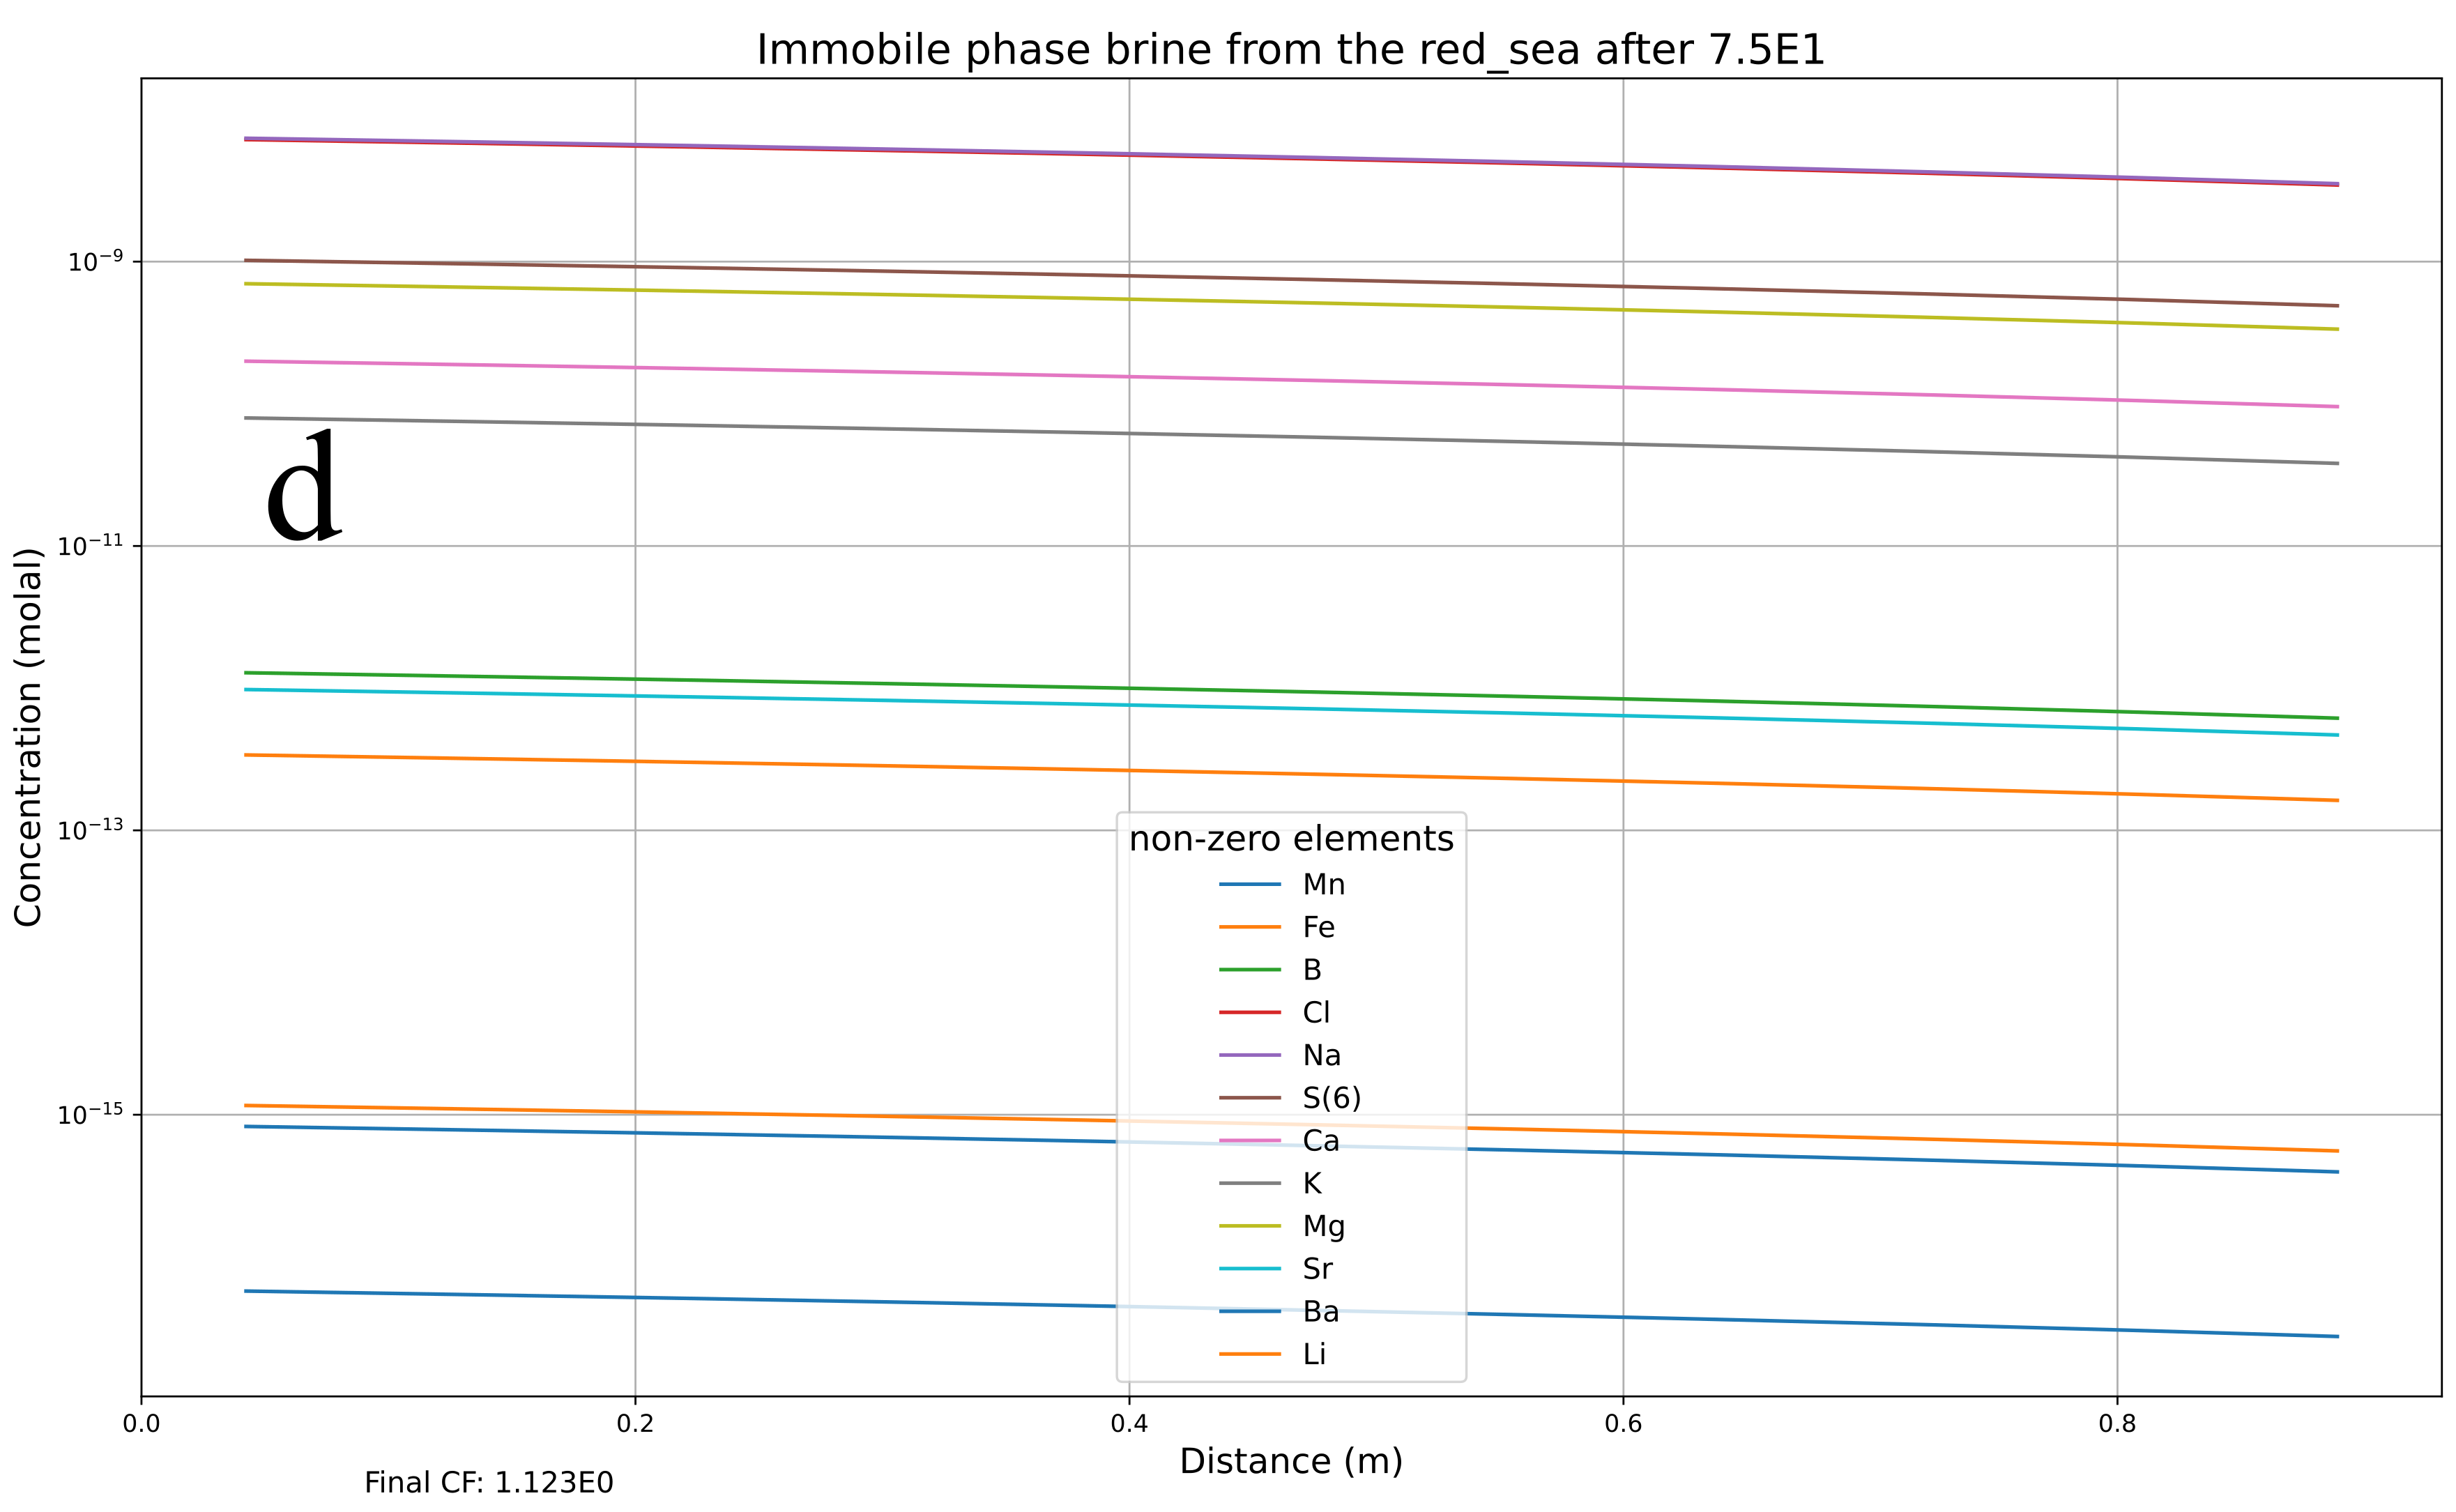
\includegraphics[width=0.49\textwidth]{images/ROSSpy/sensitivity_analyses/EF/immobile_small_ef.png} \\ \bottomrule
    \end{tabular}
    \caption{
        Counter-intuitive brine predictions from dual domain simulations with different exchange factor (EF) values, which is the $\frac{1}{s}$ rate constant of solvent exchange between the mobile and immobile solution phases. Panels a) and b) depict the mobile (bulk) and immobile (CP) phases when $EF=1E10$, while panels c) and d) depict the mobile and immobile phases when $EF=1E-10$, respectively. These non-sensible results motivated our use of the single-domain model to represent RO feed flow. 
    }
    \label{ef_values}
\end{figure}

Our model represents the feed solution with the single-domain model, despite that the dual-domain model in the module cross-section of Figure \ref{single_dual_domain} is more fundamentally accurate, since our attempts to encode the latter in PHREEQC have been unsuccessful. We represent the mobile phase (bulk solution) as one set of membrane cells -- $[1,n]~n\in W$ -- and the immobile phase (CP layer) as a separate set of cells -- $[n+2,m]~m \in W>n+2$. These cell sets exchange solvent at a parameterized rate -- the Exchange Factor $\frac{1}{s}$ (EF) -- which in Figure \ref{ef_values} is very influential upon the simulation predictions; however, the brine concentrations dilute in both solution compartments during desalination simulation. The scaling predictions are equally non-sensible. Our model therefore uses the single-domain model, which appears to be an acceptable approximation per our validations. The developer of PHREEQC -- David Parkhurst -- is uncertain whether the dual-domain model is compatible with the PHREEQ code, which assures us that the single domain model may be the best approximation of desalination reactive transport that is accessible to our open-source framework.

\begin{figure*}
    \centering
    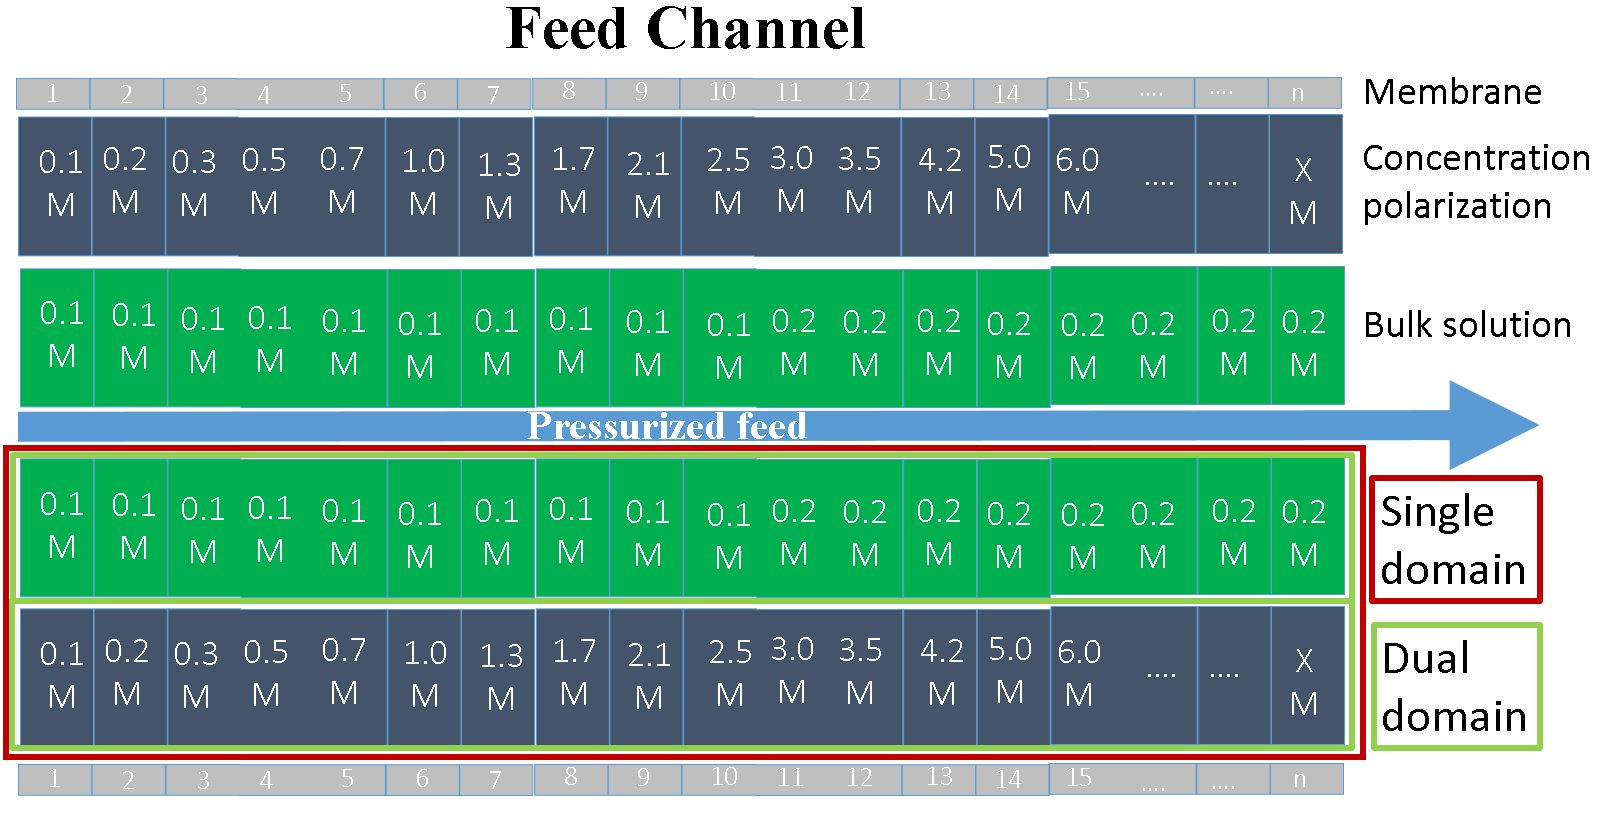
\includegraphics[width = \textwidth]{images/ROSSpy/supporting_information/single_dual_domain.jpg}
    \caption{
        A conceptual cross-section of the RO module. The membrane layers on top and bottom of the figure are discretized into an arbitrary $n$ cells. The figure illustrates the reactive transport phenomena, where the feed solution progressively becomes more concentrated as it transports through the module. The CP layer becomes much more concentrated than the bulk solution as a consequence of the no-slip boundary condition, where the velocity gradient reaches zero at the membrane surface and thus does not diffuse. These bulk and CP solutions are resolved in the dual-domain model (green boxed regions) and are granulated into a single solution by the single-domain model (red boxed regions). The latter was implemented in our model by necessity of PHREEQC.
    }
    \label{single_dual_domain}
\end{figure*}

\subsection{PHREEQ}
The most pertinent calculations of PHREEQC for our model are summarized in the following sub-section, while the version 3 PHREEQC User's manual provides a rigorous description of all PHREEQC operations.

\subsubsection{PHREEQ calculations}
\subsection{PHREEQ calculations}
The total concentration $\Psi_i$ of ionic species $i$ is calculated in each timestep, 
\begin{equation} \label{total_species_concentration}
    \Psi_i=C_i+\sum_{j=1}^{J}(v_{ij}*C_j),
\end{equation}
where $C_i$ is the molal concentration of dissolved $i$; $J$ is the set of compounds that contain $i$; $C_j$ is the molal concentration of compound $j$ that contains $i$; and $v_{ij}$ is the stoichiometric coefficient for the moles of $i$ per mole of compound $j$. The mineral precipitation equilibria over the simulation time $t$ is calculated through a similar equation, 
\begin{equation} \label{concentration_change}
    \frac{\partial \Psi_i}{\partial t}=\sum_{m=1}^{N_m}(v_{mj}*R_m),
\end{equation}
where $N_m$ is the set of reactions that include specie $i$; $v_{mj}$ is the stoichiometric coefficient for the moles of $i$ per mole of mineral $m$; and $R_m$ is the reaction flux of dissolution or precipitation for $(+)$ and $(-)$, respectively,
\begin{equation} \label{mineral_precipitation_reaction}
    R_m=sgn[\Omega]*A_m*k_m*(\Pi(a^n)) |e^{\frac{\eta*\Delta G}{RT}}-1|^p,
\end{equation}
where $\Omega = log\left(⁡\frac{Q_{dissolution}}{K_{sp}}\right)$ and, for the simulated mineral $m$, $A_m$ is the reacting surface area; $k_m$ is the rate constant of dissolution or precipitation; $Q_m$ is the ion activity product constant; and $\eta$ and $p$ are experimentally determined parameters. The $|e^{\frac{\eta * \Delta G}{RT}}-1|^p$ term simplifies to $1$ for irreversible precipitation or dissolution. The set of \cref{total_species_concentration,concentration_change} necessitates that any perturbations to ionic concentrations $\frac{\partial \Psi_i}{\partial t}$ manifest from complexation equilibria. The molal concentration $C_j$ of compound $j$ is discerned,
\begin{equation}
    C_j=\frac{\Pi_{j=1}^{N_c} (\gamma_j*K_j )^{v_{ij}}}{\gamma_j*K_j},
\end{equation}
where $N_c$ is the set of linearly independent chemical reactions; $\gamma_j$ is the activity coefficient of compound $j$; and $K_j$ is the equilibrium constant
\begin{equation}
    K_j=a_j \Pi_m^{M_{aq}} (a_m)^{-v_{m,j}},
\end{equation}
where $M_{aq}$ is the number of minerals in the aqueous system; $v_{m,i}$ is the stoichiometric coefficient of compound $j$ per mole of mineral $m$; and $a_j$ and $a_m$ are the activity coefficients of compound $j$ and mineral $m$, respectively. The activity coefficient $\gamma_j$ is calculated through either the Debye-Hückel model \cite{Aqion2016ActivityModels},
\begin{equation}
    log⁡(\gamma_j)=-A*z_j^2\sqrt{\mu},
\end{equation}
the WATEQ Debye-Hückel model \cite{Aqion2016ActivityModels},
\begin{equation}
    log⁡(\gamma_j)=\frac{-A*z_j^2*\sqrt{\mu}}{1+B*a_j^0*\sqrt{\mu}}+b_j \mu,
\end{equation}
the Davies model \cite{Davies1938TheSulphates},
\begin{equation}
    log⁡(\gamma_j)=-A*z_j^2 (\frac{\sqrt{\mu}}{1+\sqrt{\mu}}-0.2\mu),
\end{equation}
or the empirical Pitzer model \cite{Pitzer1973ThermodynamicsEquations}, where $A$ and $B$ are experimentally determined parameters; $a_j^0$ and $b_j$ are fitted parameters; $z_j$ is the charge of compound $j$; and $\mu$ is the ionic strength of the solution
\begin{equation}
    \mu=\frac{1}{2}\sum_{j=1}^{N_{aq}}z_j^2 \frac{n_j}{W_{aq}},
\end{equation}
where $W_{aq}$ is the simulated water mass and $n_j$ 
\begin{equation}
    n_j=C_j*W_{aq}=\frac{K_i*W_{aq}}{\gamma_j*(\Pi_m^{M_{aq}} (a_m)^{v_{m,j}}}
\end{equation}
is the moles of compound $j$. These calculations and geochemical models are more thoroughly described in the PHREEQC manual and in the cited literature.


\end{supplementary}

\newpage
\startchapter{A kinetic model and API of PDI}
\label{PDIpy_chapter}

\section{Introduction}
Antibiotic resistant infections are projected to exceed cancer in annual deaths, and globally cost $10^{13}~USD$ in lost economic production, by mid-21st century \cite{ONeill2014AntimicrobialNations}. Methicillin-resistant \textit{Staphylococcus aureus} (MRSA) \cite{Song2011SpreadStudy,Borg2007PrevalenceCountries} and fluoroquinolone-resistant \textit{Salmonella} \cite{Moghnieh2018EpidemiologyLeague} are two worrisome examples of virulent pathogens that are developing resistance to the antibiotics that subdued them during the 20th century. Antimicrobial resistance (AMR) evolution can be slowed by reducing excessive and incomplete use of antibiotics for human illness and animal agriculture (which is globally the primary consumer of antibiotics \cite{VanBoeckel2017ReducingAnimals,Eggleton2020TheWorld}); however, the fundamental cause of AMR is the conventional strategy of targeting a specific microbial vulnerability. This high selectivity can mitigate off-target effects, however, it places evolutionary pressure on the pathogen to fortify the targeted biochemical vulnerability and thus become immune to the treatement. This arms race of medicinal chemists against microbial evolution must therefore be replaced with a more efficient and sustainable medical strategy, and one that ideally also avoids the persistent ecotoxicity  \cite{Thomas2001AntifoulingEffects,Niu2016RolesIrradiation,Winters1983ControlDesalination}.

\subsection{Photodynamic inactivation}

Photodynamic inactivation (PDI), which differs from photodynamic therapy (PDT) for cancer treatment \cite{Lange2019ComparisonLines} only in its application, offers an effective alternative for treating prokaryotic \cite{Hamblin2004PhotodynamicDisease} and viral \cite{Wigginton2010OxidationInactivation,Lebedeva2020TheViruses} pathogens. PDI describes a photochemical process where reactive oxygen species (ROSs) \cite{Zepp1992HydroxylReaction,Koppenol2001TheLater}, primarily singlet state oxygen ($\ce{^1O2}$, the lowest excitation state of diatomic oxygen) \cite{Ergaieg2008InvolvementPorphyrin, Allen2004IntroductionSimulations, Henze2019Multi-scaleCheckpoint, Zaman2005ComputationalMatrices,Gillespie2007StochasticKinetics}, non-selectively oxidize biological substrate \cite{Choe2006MechanismsOxidation,Frankel1980LipidOxidation}. This mechanism enables PDI to simultaneously 1) avoid resistance evolution \cite{Tavares2010AntimicrobialTreatment,Lauro2002PhotoinactivationConjugates,Pedigo2009AbsenceTherapy}; 2) treat recalcitrant biofilms \cite{Beirao2014PhotodynamicPorphyrin,Ghorbanzadeh2020ModulationModel}, where the biofilm matrix is itself oxidized by $\ce{^1O2}$; and 3) avoid ecological presistence, since $\ce{^1O2}$ has only a $\approx 100 nm$ diffusion distance and a $\approx 10^{-6} s$ lifetime \cite{Moan1984TheOxygen, Moan1990OnTissues,Rodgers1982LifetimeMeasurements} in aqueous environments. The last quality encourages the use of PDI in wastewater treatment \cite{Kohn2007AssociationOxygen,Mostafa2013SingletMatter,Jimenez-Hernandez2006SolarSensitizers} and surfaces \cite{McCoy2014PhotodynamicControl} or industrial polymers \cite{Kim2003DesignProblem} where $\ce{^1O2}$ won't leach into the environment or human consumables. 

The distinction between $\ce{^1O2}$ and triplet state oxygen ($\ce{^3O2}$, the ground conformation of diatomic oxygen) is explained by their quantum multiplicities. The singlet state, of any molecule, contains only paired electrons (couples of electrons with up and down spins) and is named after its multiplicity of $1$: from 
\begin{equation} \label{multiplicity}
    multiplicity = 2(S)+1
\end{equation}
when $S=0$. The $S$ variable in \cref{multiplicity} describes the total angular momentum of the molecule -- the sum of electron spins, where up is $+\frac{1}{2}$ and down is $-\frac{1}{2}$ -- which in the case of a singlet molecule is 0 since the complete pairing of electrons necessitates that the quantities of up and down electrons are equivalent (Figure S1). The molecular triplet state, in contrast, contains two unpaired (radical) electrons that result in a multiplicity of $3$ from $S=1$ in \cref{multiplicity}. These unpaired electrons in $\ce{^3O2}$ increase shielding of the nuclear charges \cite{Katriel1972ARule} and consequently stabilize $\ce{^3O2}$ by $0.98$ eV \cite{Jockusch2008SingletExcitation} relative to $\ce{^1O2}$ that contains lacks this shielding.

The excitation of $\ce{^3O2}$ to $\ce{^1O2}$ is controlled and augmented in PDI by photosensitizer catalysts (PSs). The PS advantageously 1) is a means of localizing oxidation, 2) is a means of controlling the timing and magnitude of excitation; and 3) is a means of generating antimicrobial concentrations of $\ce{^1O2}$ that would not occur by direct excitation $\ce{^3O2 ->[{hv}] ^1O2}$ \cite{Krasnovsky2012PhotochemicalEnvironment}, since the formal selection rules \cite{Bowen1936ForbiddenLines} describe that likely excitations are those which preserve the electronic state: i.e. ground triplet to excited triplet. The $\ce{^3O2}$ could potentially excite to another triplet state and then relax into $\ce{^1O2}$ \cite{Long2003SelectionOxygen}; nevertheless, the PS catalyst accelerates $\ce{^3O2}$ excitation through energy transfers \cite{You2018ChemicalOxygen,Schalk2008Near-infraredTetratolyl-porphyrins,Jockusch2008SingletExcitation}.

The first mechanistic step of PDI describes the ground-state PS ($\ce{^1PS}$) absorbing a photon ($hv$) and entering an excited singlet state ($\ce{^1PS^*}$), according to the selection rules. This excited state then relaxes through intersystem crossing, instead of fluorescing \cite{Kessel1982DeterminantsSpectra}, to an excited triplet state ($\ce{^3PS}$),
\begin{equation} \label{ps_excitation_steps}
    \ce{^1PS <=>[{excitation}][{fluorescence}] ^1PS^* ->[][{intersystem-crossing}] ^3PS}~.
\end{equation}
The second step describes relxation via an energy transfer from $\ce{^3PS}$ to $\ce{^3O2}$, instead of phosphorescence \cite{Mcrae1958Enhancement6}, and thereby generates $\ce{^1O2}$ while regenerating the ground-state $\ce{^1PS}$ catalyst,
\begin{equation} \label{excited_ps_steps}
    \ce{^1 PS <-[{phosphorescence}] ^3 PS ->[^3O2] ^1 PS + ^1O2}
\end{equation}
The combined efficiency of \cref{ps_excitation_steps,excited_ps_steps} is encapsulated in a quantum yield of $\ce{^1O2}$ production \cite{Bakalova2004QuantumPhotosensitizers} ($0\le \Phi_{\ce{^1O2}}\le 1 ~;~ \frac{\ce{^1O2} ~molecules ~produced}{photon ~absorbed}$). The $\ce{^3PS}$ and $\ce{^1O2}$ excited states engage in energy transfers instead of $\ce{^1PS^*}$ and $\ce{^3O2^*}$ since they have longer lifetimes as a consequence of fluorescence being more favorable than phosphorescence. The third step and final of PDI describes $\ce{^1O2}$ reacting with biological substrates through Type II oxidation mechanisms, which are concerted Schenck \cite{Prein1996TheApplications} or Alder-ene \cite{Fernandez-torquemada2012DispersionPlants} reactions that produce organic peroxides \cite{Foote1965ChemistrySelectivity}, as opposed to Type I mechanisms \cite{Bolland1949KineticsOxidation,Farmer1943TheRubber,Grynova2011RevisingAutooxidation} that only affect radical substrates \cite{Litwinienko1999DifferentialEsters}. The Type II mechanism most readily affects allylic positions of unsaturated molecules \cite{Ellison1996ThermochemistryIons,Sehon1950TheRadical}, although, saturated molecules, like those in bacterial phospholipids \cite{ODonnell1985NumericalStaphylococci}, are also oxidized by $\ce{^1O2}$,. 

\begin{figure}[t]
    \centering
    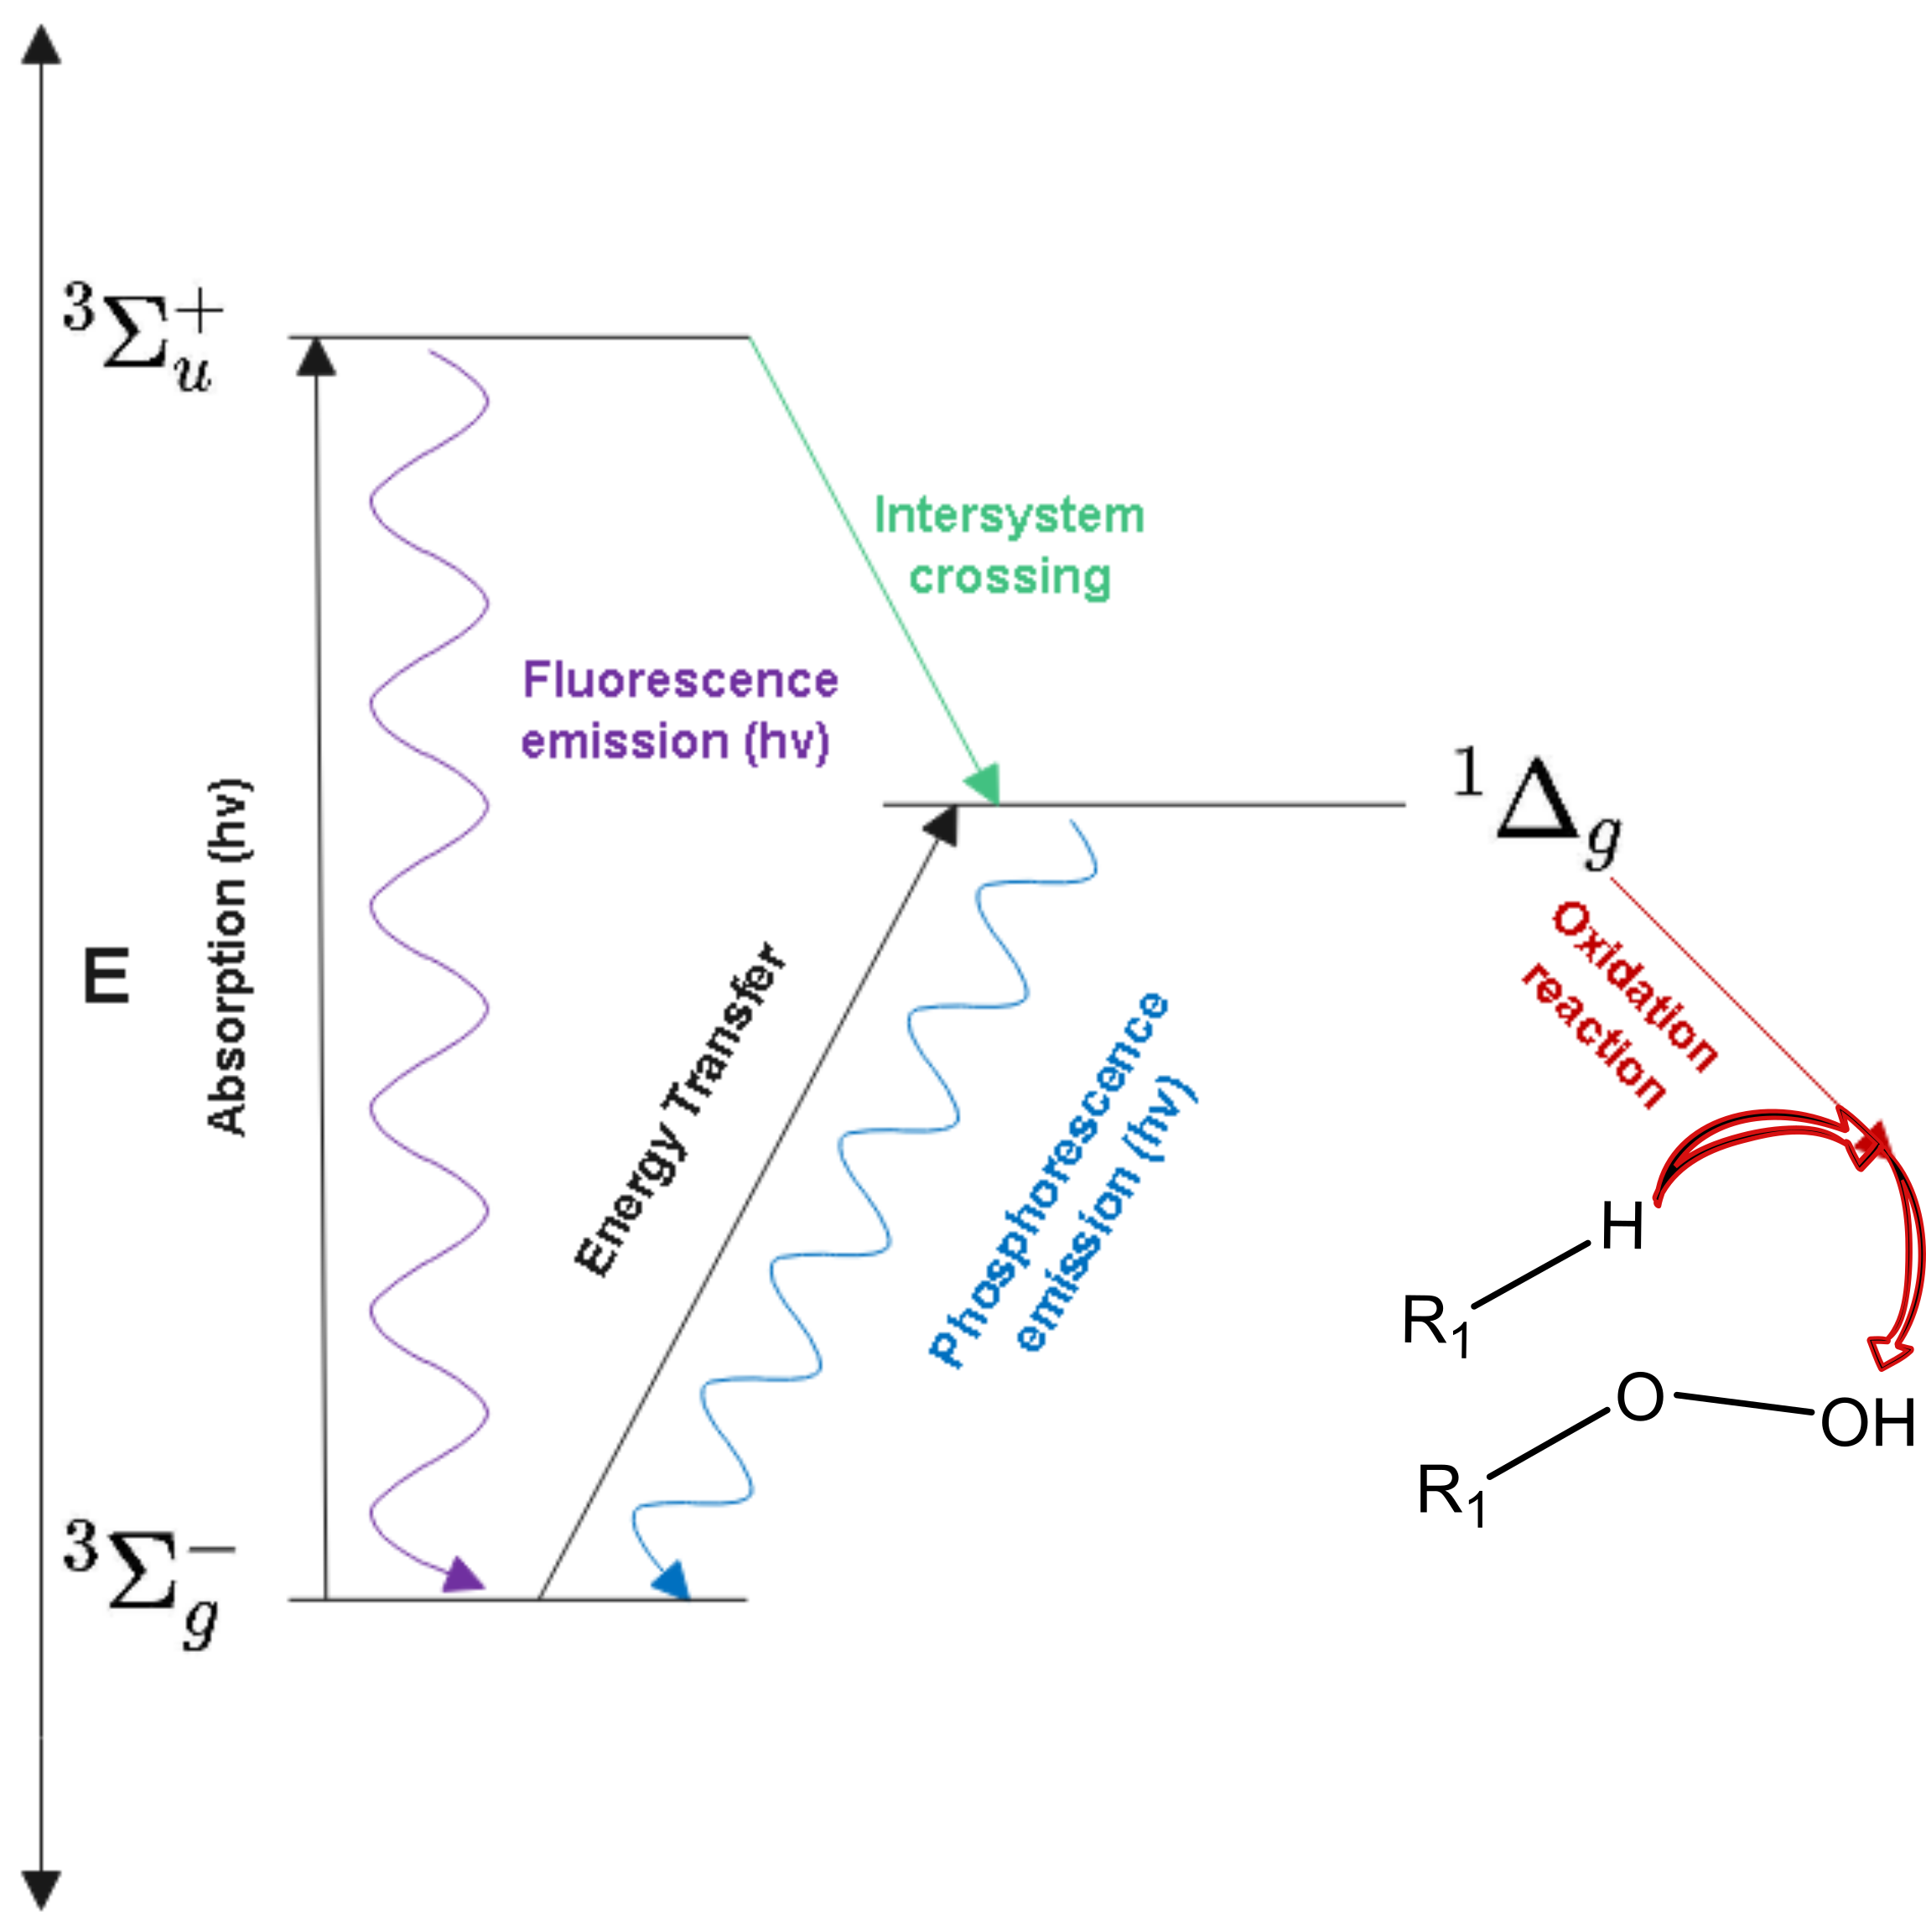
\includegraphics[width = \textwidth]{images/PDIpy/background/jablonski_diagram.png}
    \caption{
        A qualitative Jablonski energy diagram of photosensitization. The initial electronic absorption of a photon ($h\nu$) by $\ce{^3O2}$ forms a $\ce{^3O2}$* molecule, following the selection rules of excitation, which is followed with either fluorescence relaxation or an intersystem-crossing relaxation to form the reactive $\ce{^1O2}$. The singlet $\ce{^1O2}$ molecule either relaxes through phosphorescence or it reacts with an organic substrate to form a peroxide, like the illustrated hydroperoxide with a generic “R” organic group. 
    }
    \label{jablonski_diagram}
\end{figure}

\subsubsection{Photosensitizer}
The $\Phi_{\ce{^1O2}}$ efficiency is primarily dependent upon the chemical structure of the photosensitizer catalyst (PS), notwithstanding minor influence of the chemical conditions \cite{Kruk1998PhotophysicsLuminescence,Kullmann2012UltrafastBisporphyrin}. Two primary inefficiencies of PSs are its propensity to relax through fluorescence or phosphorescence, in Figure \ref{jablonski_diagram}, and to photobleach, where irradiation irreversibly compromises molecular absorptivity \cite{Bonnett2010ChemInformTherapy,Wasser1973TheMetallochlorins}. The functionality and charge of the PS should furthermore optimize its association with the targeted cells \cite{VanDerWal1997DeterminationBacteria,Dickson1989CellSurfaces} and minimize off-target oxidation \cite{Lambrechts2005PhotodynamicMice} and host toxicities \cite{Quishida2016PhotodynamicLight} in medical applications. Material applications of PDI \cite{Peddinti2018PhotodynamicThreat,Gottenbos2001AntimicrobialBacteria}, for applications in either biofouling or sterile medical surfaces, further require that the PS is amenable to permanent surface attachment in a manner that retains material properties \cite{McCoy2014PhotodynamicControl}. 

The PS finally influences the biological targets of PDI. Impermeable PSs, which cannot penetrate a cell, generally oxidize the cytoplasmic membrane \cite{Specht1990DepolarizationAction,Ehrenberg1993ElectricAlterations} instead of cytoplasmic contents \cite{Maisch2004AntibacterialDermatology}. This mechanism, which primarily affects the phospholipid fatty acids in Figure \ref{schenck_mechanism}, manifests in cell death through lysis \cite{Sahu2009AtomicColi,Bertoloni1987RoleCells} and generally affects gram-positive bacteria more than gram-negative bacteria \cite{Lauro2002PhotoinactivationConjugates,Merchat1996Meso-substitutedBacteria} since the latter possess a superficial lipopolysaccharide layer that protects the cytoplasmic membrane. Permeable PSs, by contrast, can penetrate a cell and thus generate $\ce{^1O2}$ within the cytoplasm where cytoplasmic chemicals \cite{Bagchi1979RoleAcriflavine} such as guanine nucleotides \cite{Prat1997Determination9,Devasagayam1991FormationOxygen} are fatally oxidized. This mechanism is more effective with prokaryotes than eukaryotes \cite{Quishida2016PhotodynamicLight}, since the latter have a nuclear membrane that protects DNA, particularly guanine, from oxidation \cite{Pereira2013PhotodynamicVitro}.

A narrow range of chemicals meet these criteria of an ideal PS. Semiconductors \cite{Nelson2002PhotoconductivityDioxide,Peiro2006PhotochemicalPreparations,Linsebigler1995PhotocatalysisResults}, and some amino acid residues \cite{Lippincott-schwartz2003PhotobleachingTechniques,Jin1995PhotolysisSolution}, can electrocatalytically generate $\ce{^1O2}$; however, these molecules are inefficient and/or impractical, particularly for medical applications. The most efficacious PS in nature is chlorophyll \cite{Ramel2012ChemicalPlants}, which is an organometallic porphyrinoid (Figure \ref{zinc_porphyrin}) that evolution has tuned for low rates of photobleaching and absorption of visible light -- specifically blue-violet radiation \cite{Mtangi2017ControlSplitting} via the Soret absorption band \cite{Carre1999FungicidalCerevisiae,Pereira2014InfluencePorphyrin,Ashkenazi2003PhotodynamicBacteria,Moan1986PorphyrinShGroups,Nitzan1992InactivationPorphyrins,Durantini2006PhotodynamicBacteria,Salmon-Divon2004MechanisticTetra-mesoN-methylpyridylporphine} and green-orange radiation \cite{Bertoloni2000PhotosensitizingCells} via the Q absorption band \cite{Bonnett1999PhotobleachingStudy,Jori2006PhotodynamicApplications,Gad2004TargetedMice,Zhao2019Porphyrin-basedAbsorption}. Chlorophyll, however, has not evolved traits that optimize its association with cellular targets or its compatibility with material surfaces; therefore, synthetic porphyrins \cite{Orenstein1997TheInfections,Beirao2014PhotodynamicPorphyrin,Merchat1996StudiesPorphyrins} that emulate the successful conjugated structure \cite{Huang2008Porphyrin-dithienothiopheneCells} of chlorophyll, while introducing other metal centers \cite{Mosinger1997QuantumPorphine} and functional handles  \cite{Hirao1999TheoreticalDerivatives,Wu2014BODIPY-basedSolution,Chacon1988SingletArachidonic} (e.g. Figure \ref{zinc_porphyrin}) that improve its utility in PDI \cite{Jager2016QScales,Karolczak2004PhotophysicalTetraphenylporphyrin,Mathai2007SingletTherapy}, is an appealing direction for PDI research. 

\begin{figure}
    \centering
    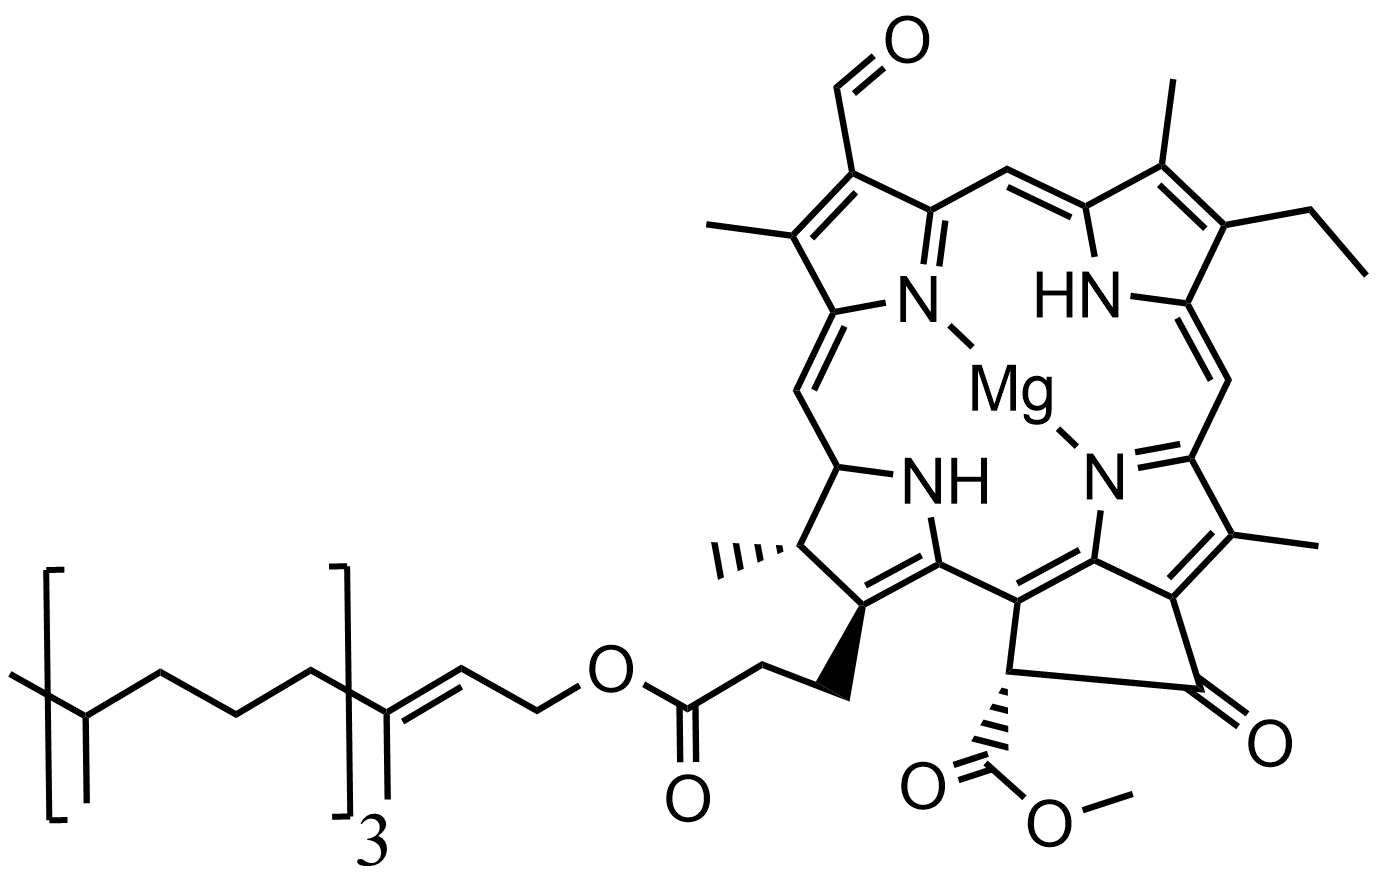
\includegraphics[width = \textwidth]{images/PDIpy/background/chlorophyll.png} \\ \midrule
    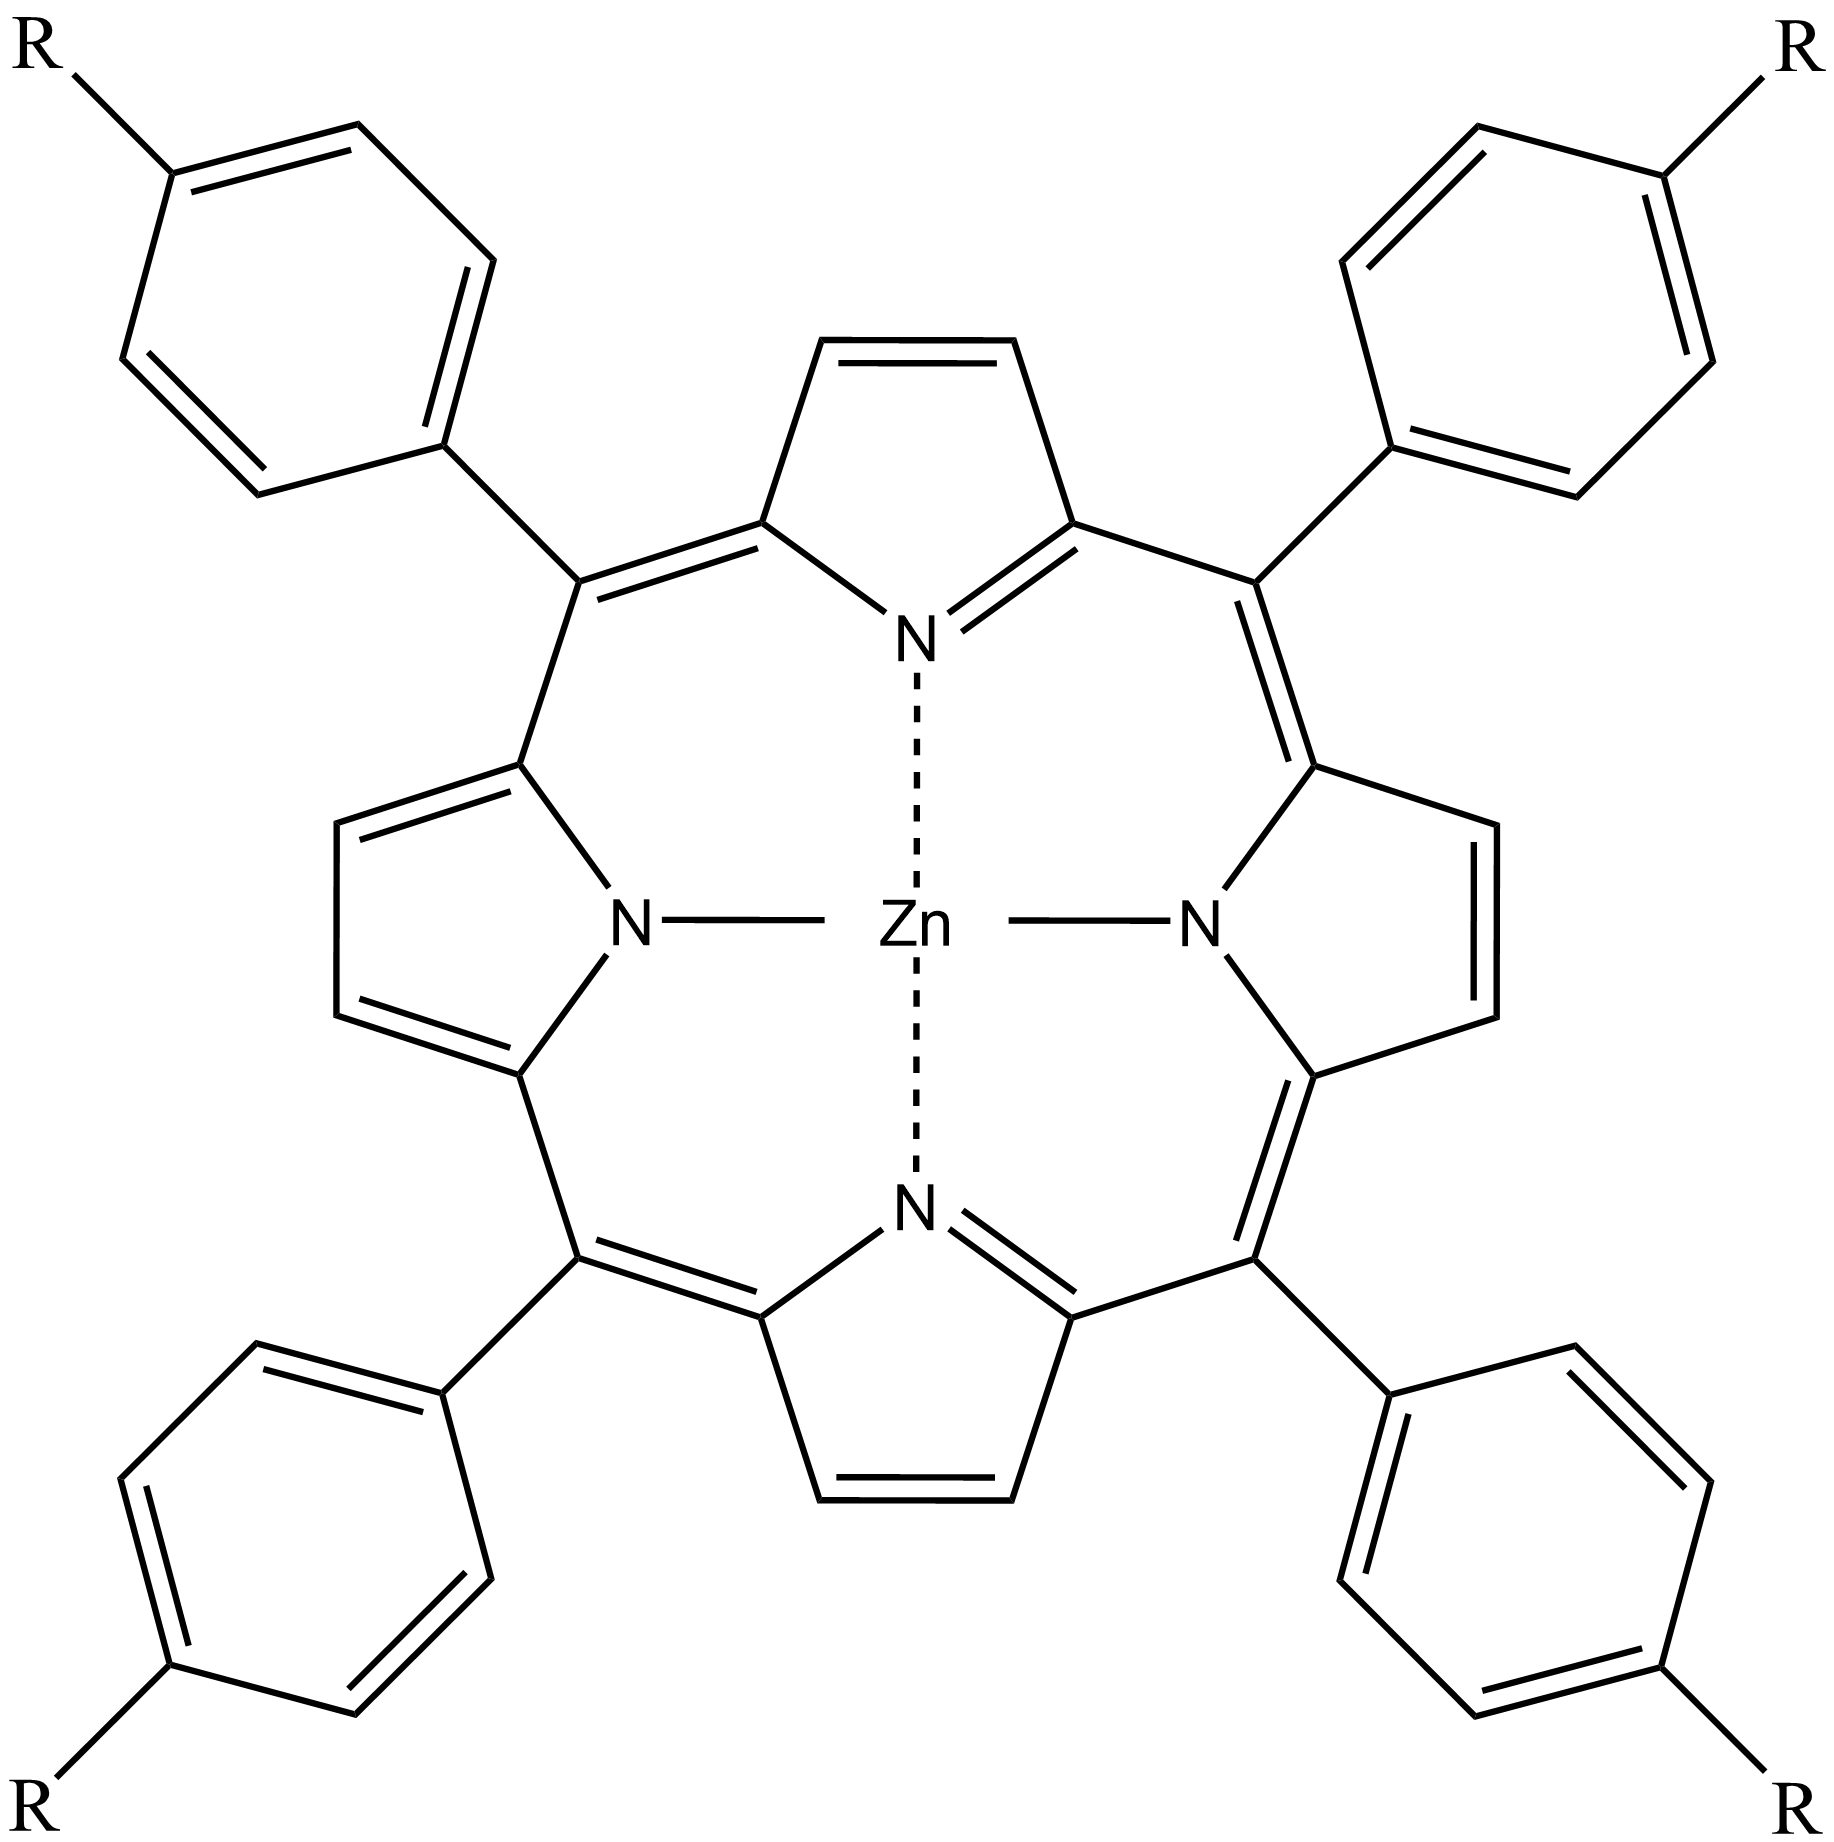
\includegraphics[width = 0.5\textwidth]{images/PDIpy/background/zinc_porphyrin.png}
    \caption{
        The chemical structure of porphyrinoid chlorophyll (top) juxtaposed with the core motif of a synthetic porphyrin analogue (bottom).
    }
    \label{zinc_porphyrin}
\end{figure}

\begin{figure}[t]
    \centering
    \includegraphics[width =0.9 \textwidth]{images/PDIpy/background/BCFA_schenck_oxidation_2.png}
    \caption{
         The Schenck reaction and associated byproduct decompositions. Step (1) depicts the concerted\cite{Foote1968PhotosensitizedOxygen} Schenck reaction. Step (2) depicts the homolytic cleavage of the hydroperoxide bond to form $\ce{OH^.}$ and an oxy radical that may enter autoxidation mechanisms. Step (3) depicts radical propagation via hydrogen abstraction to form another radical substrate and an alcohol byproduct as part of the autoxidation mechanism. Step (4) is a concerted Russell reaction\cite{Russell1957Deuterium-isotopeRadicals,Howard1968TheMechanism} between two hydroperoxides that forms a $\ce{H2O2}$, an $\alpha,\beta$-ketone, and an alcohol. The reactions of Steps (2-4) sample the wide array of possible oxidative decompositions that follow the Schenck or autoxidation mechanisms.
    }
    \label{schenck_mechanism}
\end{figure}

\subsection{PDI modeling}
Computational models of PDI that allow experimentalists, biologists and chemists alike, to explore the efficacies of different PSs and system conditions are scarce. Santos et al. \cite{Santos2020ApplicationAureus} developed a second-order polynomial to mathematically describe the inactivation of \textit{S. aureus} as a function of time at a particular wavelength and PS concentration. The predictions were demonstrated to be accurate, however, the model is bound to a narrow range of conditions, and does not permit the investigator to explore different parameters such as PS characteristics. Brasel et al. \cite{Brasel2020AnAgalactiae} developed a sigmoidal logistic model to assess the sensitivity of PDI inactivation to incident irradiance $\frac{mW}{cm^2}$ and exposure time; however, the model likewise does not permit investigations of alternative PDI systems. Finally, Sabino et al. \cite{Sabino2019InactivationTherapy} developed a Weibull power-law function from fitted inactivation data to practically predict lethal doses and the tolerance factor of a PDI system; yet, the mathematical model is limited in scope and does not describe the fundamental chemistry of PDI. 

We therefore developed a mechanistically resolved kinetic model of PDI for an impermeable PS and encapsulated into a Python API (PDIpy) that allow investigators to efficiently explore a continuum of values for numerous parameters. The means of editing and customizing the extensive list of parameters, and understanding the default values, is detailed in the API documentation. PDIpy uses Tellurium \cite{Choi2018Tellurium:Biology} to concisely construct SBML \cite{Keating2020Models}, SED-ML \cite{Waltemath2011ReproducibleLanguage}, and COMBINE OMEX \cite{Bergmann2014COMBINEProject} descriptions of the simulations and their results. These conventional formats in computational biology support transparency and reproducibility of the simulation results. The logistic (sigmoidal) Hill equation is then fitted to simulation predictions of cytoplasmic oxidation to systematically construct the inactivation plot based upon the oxidation predictions. We exemplify the model through replicating experimental studies and conducting a sensitivity analyses of key API parameters. We expect that the open-source project will foster experimental progress without expending resources, and will inspire computational biologists to refine tools for this field of medical research, towards expediting the scientific response to the looming medical crisis of antibiotic resistance. 

\section{Methods}
\subsection{Conceptual model}
PDIpy conceptually represents an experimental PDI system with a coccus (spheroid) bacterium like \textit{S. aureus}. Each simulation accepts parameters for each aspect of PDI: the light source and incident intensity; the PS absorptivity, structural dimensions, and $\frac{mol}{vol}$ or $\frac{mol}{area}$ concentration; the bacterial specie, membrane composition, and $\frac{CFU}{mL}$ for planktonic experiments; the solution dimensions; and kinetic constants for the PDI reactions. Default values for many of these parameters supplement user-defined parameters.

\subsection{Kinetic reactions}
Our model is predicated upon a set of three chemical processes that embody the essence of PDI. 1) A photoelectric interaction \cite{Wheaton2009PhotoelectricEffect} from \cref{ps_excitation_steps} occurs after $\ce{^1PS}$ is struck by a photon ($h\nu$) and undergoes intersystem crossing per to form $\ce{^3PS}$. 2) An energy transfer in \cref{excited_ps_steps} occurs from $\ce{^3PS}$ to $\ce{^3O2}$. 3) The $\ce{^1O2}$ oxidizes biological substrates, which includes both cytoplasmic phosholipids and biofilm polymeric substances, or it irreversibly disrupts PS absorptivity through photobleaching 
\begin{equation} \label{bleaching}
    \ce{^1PS -> ^1PS_{bleached}}~.
\end{equation}
A complete description of this kinetic system is represented in Table \ref{reactions_table}, and each of the reactions are each detailed in the following sub-sections.

\subsubsection{User inputs}
The PDIpy API accepts a variety of parameters that allow the user to customize almost every aspect of the PDI system. These parameters of the simulated PDI system can be provided through either a dictionary argument in the \pyobject{define\_conditions} function, or through a JSON parameter file for each category of parameters -- e.g. light, PS, bacterium, and solution space -- that elaborate the simulated system in a more reproducible and transparent manner than dictionary arguments. The complete list of accepted parameters and formats are detailed in the PDIpy documentation (\url{https://github.com/freiburgermsu/PDIpy/blob/main/README.rst}).

\begin{table}[]
    \centering
    \begin{tabular}{c|c}
        \textbf{Name} & \textbf{Reaction} \\
        \toprule
        Photoexcitation & \ce{^1PS <=> ^3PS} \\
        Photobleaching & \ce{^1PS -> ^1PS_{bleached}} \\
        Energy transfer & \ce{^3PS + ^3O2 -> ^1PS + ^1O2} \\
        Phosphorescence & \ce{^1O2 -> ^3O2} \\
        Membrane oxidation & \ce{^1O2 + FA -> oFA} \\
        EPS oxidation & \ce{^1O2 + EPS -> oEPS} \\
    \end{tabular}
    \caption{
        Each of the chemical reactions that define the PDI model of PDIpy. These reactions are individually detailed in dedicated subsections.
    }
    \label{reactions_table}
\end{table}

\subsubsection{Photoelectric}
\paragraph{PS excitation}
PDI begins with the excitation of the PS. This occurs as the combined result of an incident photon i) entering the aqueous solution, ii) striking a PS, and then iii) exciting an electron. This sequence is encapsulated in the kinetic expression
\begin{multline} \label{ps_excitation_kinetics}
    \frac{d[\ce{^3PS}]}{dt} =  k_{excitation}*\frac{photons_{PS}}{photons_{total}} \\ 
    *\Phi_{excitation}*[\ce{^1PS}] - k_{fluorescence}*[\ce{^3PS}]~. 
\end{multline}
The $k_{excitation}$ \& $k_{fluorescence}$ rate constants are estimated as the inverse of the rise and decay times for the selected PS, respectively. The approximate rise time for a porphyrin PS is $50 fs$, which is consistent with estimates of $<100 fs$ \cite{Andersson1999PhotoinducedState} and $60-90 fs$ in ethanol solvent \cite{Gurzadyan1998Time-resolvedZn-tetraphenylporphyrin} which elongates the lifetime of excited molecules relative to water. The decay time, as the S2 fluorescence \cite{Akimoto1999UltrafastPorphyrins}, and $\Phi_{excitation}$ ($\frac{PS excited}{photon absorbed}$) are approximated for a porphyrin PS as $1.5 ns$ and $\approx 0.7$ \cite{Krasnovsky2012PhotochemicalEnvironment}, respectively. The $\frac{photons_{PS}}{photons_{total}}$ \cite{Brasel2020AnAgalactiae}, which is the proportion of photons in the solution that strike a photosensitizer, is calculated through a series of steps. 1) The reported intensity of incident light from the respective light source -- i.e. either irradiance ($\frac{mW}{cm^2}$), lux ($\frac{lumen}{m^2}$), or lumens (lumens) -- is converted into $watts_{incident}$ ($\frac{J}{s}$). 2) This wattage is attenuated by the proportion of the emission spectrum $light_{incident}$ that resides within the excitation spectrum of the parameterized photosensitizer $light_{excitation}$, 
\begin{equation}
    watt_{excitation} = \frac{light_{excitation}}{light_{incident}}*watts_{incident}.
\end{equation}
3) The $watt_{excitation}$ is used to calculate the moles of incident photons that strike photosensitizers per timestep 
\begin{multline} \label{photons_per_second}
    \frac{photons_{PS}}{timestep}=\frac{<h\nu_{excitation}>}{h*c}*watts_{excitation} \\
    *\frac{second}{timestep}*reflection*scattering*\frac{1 mole}{N_A}*\frac{vol_{PS}}{vol_{total}},
\end{multline}
where $reflection \approx 96 \%$ represents the proportion of incident photons that penetrate an aqueous solution \cite{Gross1993SingletLiposomes}; and $scattering$ represents the proportion of light that reaches a specified depth \cite{RobertW.1973TheSea}, which is calculated by 
\begin{equation}
    I_z = I_0*e^{-k*z}~,
\end{equation}
where $I_z$ is the light intensity relative to the $I_0$ after depth $z$, and $k$ is the attenuation coefficient, which is $\approx 0.04~(\frac{1}{m})$ \cite{Lorenzen1972ExtinctionPhytoplankton} for clear waters. The $\frac{vol_{PS}}{vol_{total}}$ represents the volume proportion of the PS ($vol_{PS}$) -- calculated as the product of the quantity of PS molecules and the volume per molecule per its structure -- to the total volume of the solution in which the PS resides ($vol_{total}$) \cite{Santos2020ApplicationAureus}. The average excitation wavelength of the PS ($<h\nu_{excitation}>$) is calculated as the weighted average of the Soret and Q excitation bands, in proportion to their relative contribution in generating $\ce{^1O2}$ \cite{Nitzan2001PhotoinactivationWavelengths,Hoenes2020PhotoinactivationWavelength}, since this averaged wavelength simultaneously embodies contributions of both excitation bands. The resultant $\frac{photons_{PS}}{timestep}$ from \cref{photons_per_second} is then divided by the $\frac{photons_{total}}{timestep}$ to complete the kinetic expression in \cref{ps_excitation_kinetics} that calculates the excitation of PS in each timestep. 

\paragraph{Photobleaching}
The collision of a PS and a photon may alternatively disrupt the conjugated PS system and prevent further excitation, which is depicted in \cref{bleaching}. The kinetic expression 
\begin{equation} \label{bleaching_kinetics}
    \frac{d[\ce{^1PS_{bleached}}]}{dt} = k_{bleaching}*[\ce{^1PS}]*[\ce{^1O2}]~,
\end{equation}
represents this process. The $k_{bleaching}$ rate constant for the oxygen-dependent photobleaching reaction of \cref{bleaching_kinetics} -- as opposed to the oxygen-independent, first-order, photobleaching reaction \cite{Bonnett1999PhotobleachingStudy,Mang1987PhotobleachingTherapy} -- possesses a rate constant of $\approx 600 \frac{cm^2}{J*M}$ \cite{Dysart2005CalculationCells} for porphyrins, which is a function of light exposure $\frac{J}{cm^2}$.

\subsubsection{Energy Transfer}
The energy transfer from $\ce{^3PS}$ to $\ce{^3O2}$  in \cref{excited_ps_steps} is described with by the kinetics expression
\begin{equation} \label{energy_transfer_kinetics}
    \frac{d[\ce{^1O2}]}{dt} = k_{transfer}*\Phi_{transfer}*[^3PS]*[\ce{^3O2}]. 
\end{equation}
The rate constant $k_{transfer}$ is the inverse of the decay time of $\ce{^3PS}$, which for a porphyrin PS appears to be $100 ns$ in aqueous after accounting for the reported value \cite{Kupper2002KineticsOxygen} in acetone solvent that significantly increases the lifetime of excited states \cite{Spikes1992QuantumUroporphyrin}. The $\ce{^1O2}$ phosphorescence side reaction, which often emits a specific infrared wavelength that can be measured to approximate the $[\ce{^1O2}]$ \cite{Macpherson1993DirectCentres}, is kinetically represented 
\begin{equation}
    \frac{d[\ce{^3O2}]}{dt} = k_{phosphorescence}*[\ce{^1O2}]
\end{equation}
where $k_{phosphorescence}$ is a function of $\frac{CFU}{mL}$, since the $\ce{^1O2}$ lifetime is greater in biological material and thus it is proportional with the bacterial concentration in planktonic simulations \cite{Maisch2007TheBacteria}. The minimum lifetime is limited to $3.5\mu s$ for pure water \cite{Baier2005Time-resolvedCells}.

\subsubsection{Oxidation}
The oxidation reactions are the primary consumers of oxygen in the kinetic system. The simulated system, however, is assumed to possess an equilibrium between the solution and the atmosphere, which prevents the depletion of oxygen in the system. This is represented by replacing each oxygen molecule that is consumed during the oxidation of biological substrate in \cref{membrane_oxidation,EPS_oxidation}.

\paragraph{Cytoplasmic membrane} 
The oxidation of cytoplasmic phospholipids, which we approximate as fatty acid chains, is represented as an irreversible second-order reaction \cite{Watabe2007OxidationMembranes.}
\begin{equation} \label{membrane_oxidation}
    \ce{^1O2 + FA -> oFA}.
\end{equation}
and a second-order kinetic expression
\begin{equation} \label{membrane_oxidation_kinetics}
    \frac{d[oFA]}{dt} = k_{fa}*[\ce{^1O2}]*[FA]~.
\end{equation}
The rate constant $k_{fa} \approx 769 \frac{L}{g*s}$ \cite{Mukai2019KineticSolution} and the concentration of fatty acid chains in the cytoplasmic membrane is described in units of $\frac{g}{L}$, after calculating the weighted average MW of fatty acids within the membrane. 

\paragraph{Biofilm matrix} 
The oxidation of EPS is reported to be significant during PDI \cite{Beirao2014PhotodynamicPorphyrin}. This process is represented through an irreversible reaction
\begin{equation} \label{EPS_oxidation}
    \ce{^1O2 + EPS -> oEPS},
\end{equation}
which competes with \cref{membrane_oxidation} for $\ce{^1O2}$ and thereby lessens the efficacy of PDI upon biofilms relative to planktonic organisms. The oxidation of bioiflm polymers is kinetically represented  
\begin{equation} \label{EPS_oxidation_kinetics}
    \frac{d[oEPS]}{dt} = k_{EPS_{oxidation}}*[\ce{^1O2}]
\end{equation}
with an empirical rate constant that we approximated as $37.75~\frac{1}{s}$ for \textit{S. aureus}, and an initial concentration of EPS that is $9x$ greater than the cellular mass, in proportion to mass distributions of biofilms \cite{Flemming2010TheMatrix}.

\subsection{Inactivation fitting}

Simulation results of chemical concentrations over time are processed into predictions of bacterial inactivation through a series of mathematical steps. 1) The proportion of oxidized substrate
\begin{equation} \label{oxidation_proportion}
    ox_{proportion} = \frac{[oFA]}{[oFA]+[FA]}
\end{equation}
is fitted to a sigmoidal curve, similar to other models \cite{Xiong1999AInactivation}. We used the signmoidal Hill-equation \cite{Gesztelyi2012ThePharmacology} as a biochemical kinetic model that derives from mass-action kinetics similar to the Michaelis-Menten kinetic model, however, a fitting module for the Hill-equation did not exist; hence, the HillFit Python module was developed with a variation of the Hill-equation \cite{Inoue2016OscillationActivation} 
\begin{equation} \label{hill_eq}
    y=bottom+\frac{(top-bottom)*x^n}{EC50^n+x^n}~,
\end{equation}
that improves its fit to data, to fit the oxidation data from PDIpy simulations. The regression parameters from the fitted Hill equation are then systematically adjusted to construct an inactivation plot that replicates experimental results while preserving the underlying Hill-equation relationship. These parameter adjustments are presented in Table \ref{hill_parameters} for both simulations of planktonic and biofilm bacteria, since biofilms factors such as impaired diffusion that are not explicitly accounted in our kinetic model and thus must be compensated through other means. The top parameter of \cref{hill_eq} is adjusted asymptotically to a limit that follows an subtly different empirical expression for planktonic $1-10^{-\Omega}$ than biofilm $1-10^{-0.7-\Omega }$ simulations, where $\Omega = wattage^{\frac{1}{5}}-log10(1-final_{oxidation\_proportion})$. This top limit is empirically determined to manifest in the log-inactivation predictions being 1-2 greater than the log-oxidation from \cref{oxidation_proportion}, which embodies our assumption -- and an implicit observation in experimental studies -- that $1-10\%$ of membrane phospholipids must experience oxidation for the cell to lyse. 

\begin{table}[]
    \centering
    \begin{tabular}{l|c|c}
        \textbf{Bacterial state} & \textbf{Hill parameter} & \textbf{Adjustment} \\
        \multirow{2}{}{Planktonic} & EC50 & -76\% \\
         & nH & +100\% \\
         \midrule
         \multirow{2}{}{Biofilm} & EC50 & -65\% \\
         & nH & +120\% \\
    \end{tabular}
    \caption{
        The Hill parameters adjustments that are enacted to create the inactivation plot for both planktonic and biofilm systems. 
    }
    \label{hill_parameters}
\end{table}

% \subsubsection{Cross-linked systems}

% \paragraph{iPDIpy}
% The PDIpy API is graphically interactive through a user interface iPDIpy, which is depicted in Figure \ref{}. This interface provides a convenient means for parameterizing a PDIpy simulation, exporting and importing sets of parameters, parsing the processed simulation data, viewing error messages and calculated values, viewing the output figure of bacterial reduction over time, and parsing the processed data through a build-in function. The iPDIpy version of PDIpy is downloadable from our GitHub repository.

% \begin{figure}
%     \centering
%     \includegraphics{}
%     \caption{
%         The left pane of the GUI will contain command buttons like restarting the simulation or export results, while the right pane will edit the simulation data and or bacterial qualities/species.
%     }
%     \label{iPDIpy_interface}
% \end{figure}


\section{Case Studies}
A PDI experiment from literature that thoroughly described its expeirmental procedure was parameterized in PDIpy to compare the predicted results with the reported results. These comparisons in the following sections all pertain to \textit{S. aureus}, which is a model coccus bacterium that is abundantly described in studies of PDI and AMR infectants as MRSA.

% \subsection{Cross-linked PS}
% Experimental data from our lab with cross-linked PSs (unpublished) was parameterized, in Table \ref{}, into PDIpy. The predicted reduction curve over time in Figure \ref{} agreed with the experimental data at the measured time of 6 hours and 98\% reduction, which supports that the software yields accurate predictions. 

% \paragraph{}
% .

\subsection{Solution PS}

\paragraph{Beirao et al.\cite{Beirao2014PhotodynamicPorphyrin}}
This paper experimentally examines the efficacy of a dissolved PS, over a range of concentrations, against both planktonic and sessile states. The ample experimental details were parameterized into PDIpy, and the predicted log-inactivation was contrasted with the reported log-inactivation at various times, concentrations, and bacterial states in Table \ref{beirao_et_al_data}. The predicted log-oxidation and log-inactivation for a few of the simulated conditions from the study are plotted in Figure \ref{beirao_et_al}, with the respective regression plots from fitting the Hill-equation to the log-oxidation results in Figure \ref{hill_regression}. The very precise fitting of the data -- $R^2 > 0.996$ -- supports that our kinetic model of PDI fundamentally recreates the biochemical relationship that is predicted by the Hill model of kinetics.

\begin{table}[h]
    \centering
    \begin{tabular}{c|c|c|c|c|c}
        Bacterial & [PS] & Inactivation & Reported & Predicted & \multirow{2}{1.2cm}{\%-error}\\
        state & ($\mu m$) & (-log10) & (min) & (min) & \\
        \toprule
        \multirow{3}{1.5cm}{planktonic} & 5 & 7.6 & 51 & 117 & 119\\
        & 10 & 7.6 & 51 & 36 & -29\\
        & 20 & 7.6 & 42 & 12 & -71\\
        \midrule
        \multirow{3}{1.5cm}{sessile} & 5 & 3.6 & 390 & 566 & 45\\
        & 10 & 5 & 390 & 310 & -20\\
        & 20 & 6.3 & 390 & 247 & -37\\
        \bottomrule
    \end{tabular}
    \caption{
        A quantitative comparison of published inactivation data, with both planktonic and sessile, \textit{S. aureus}, with predictions from PDIpy. The \%-error for each prediction is provided in the table as a metric of accuracy
    }
    \label{beirao_et_al_data}
\end{table}

\begin{figure}
    \centering
    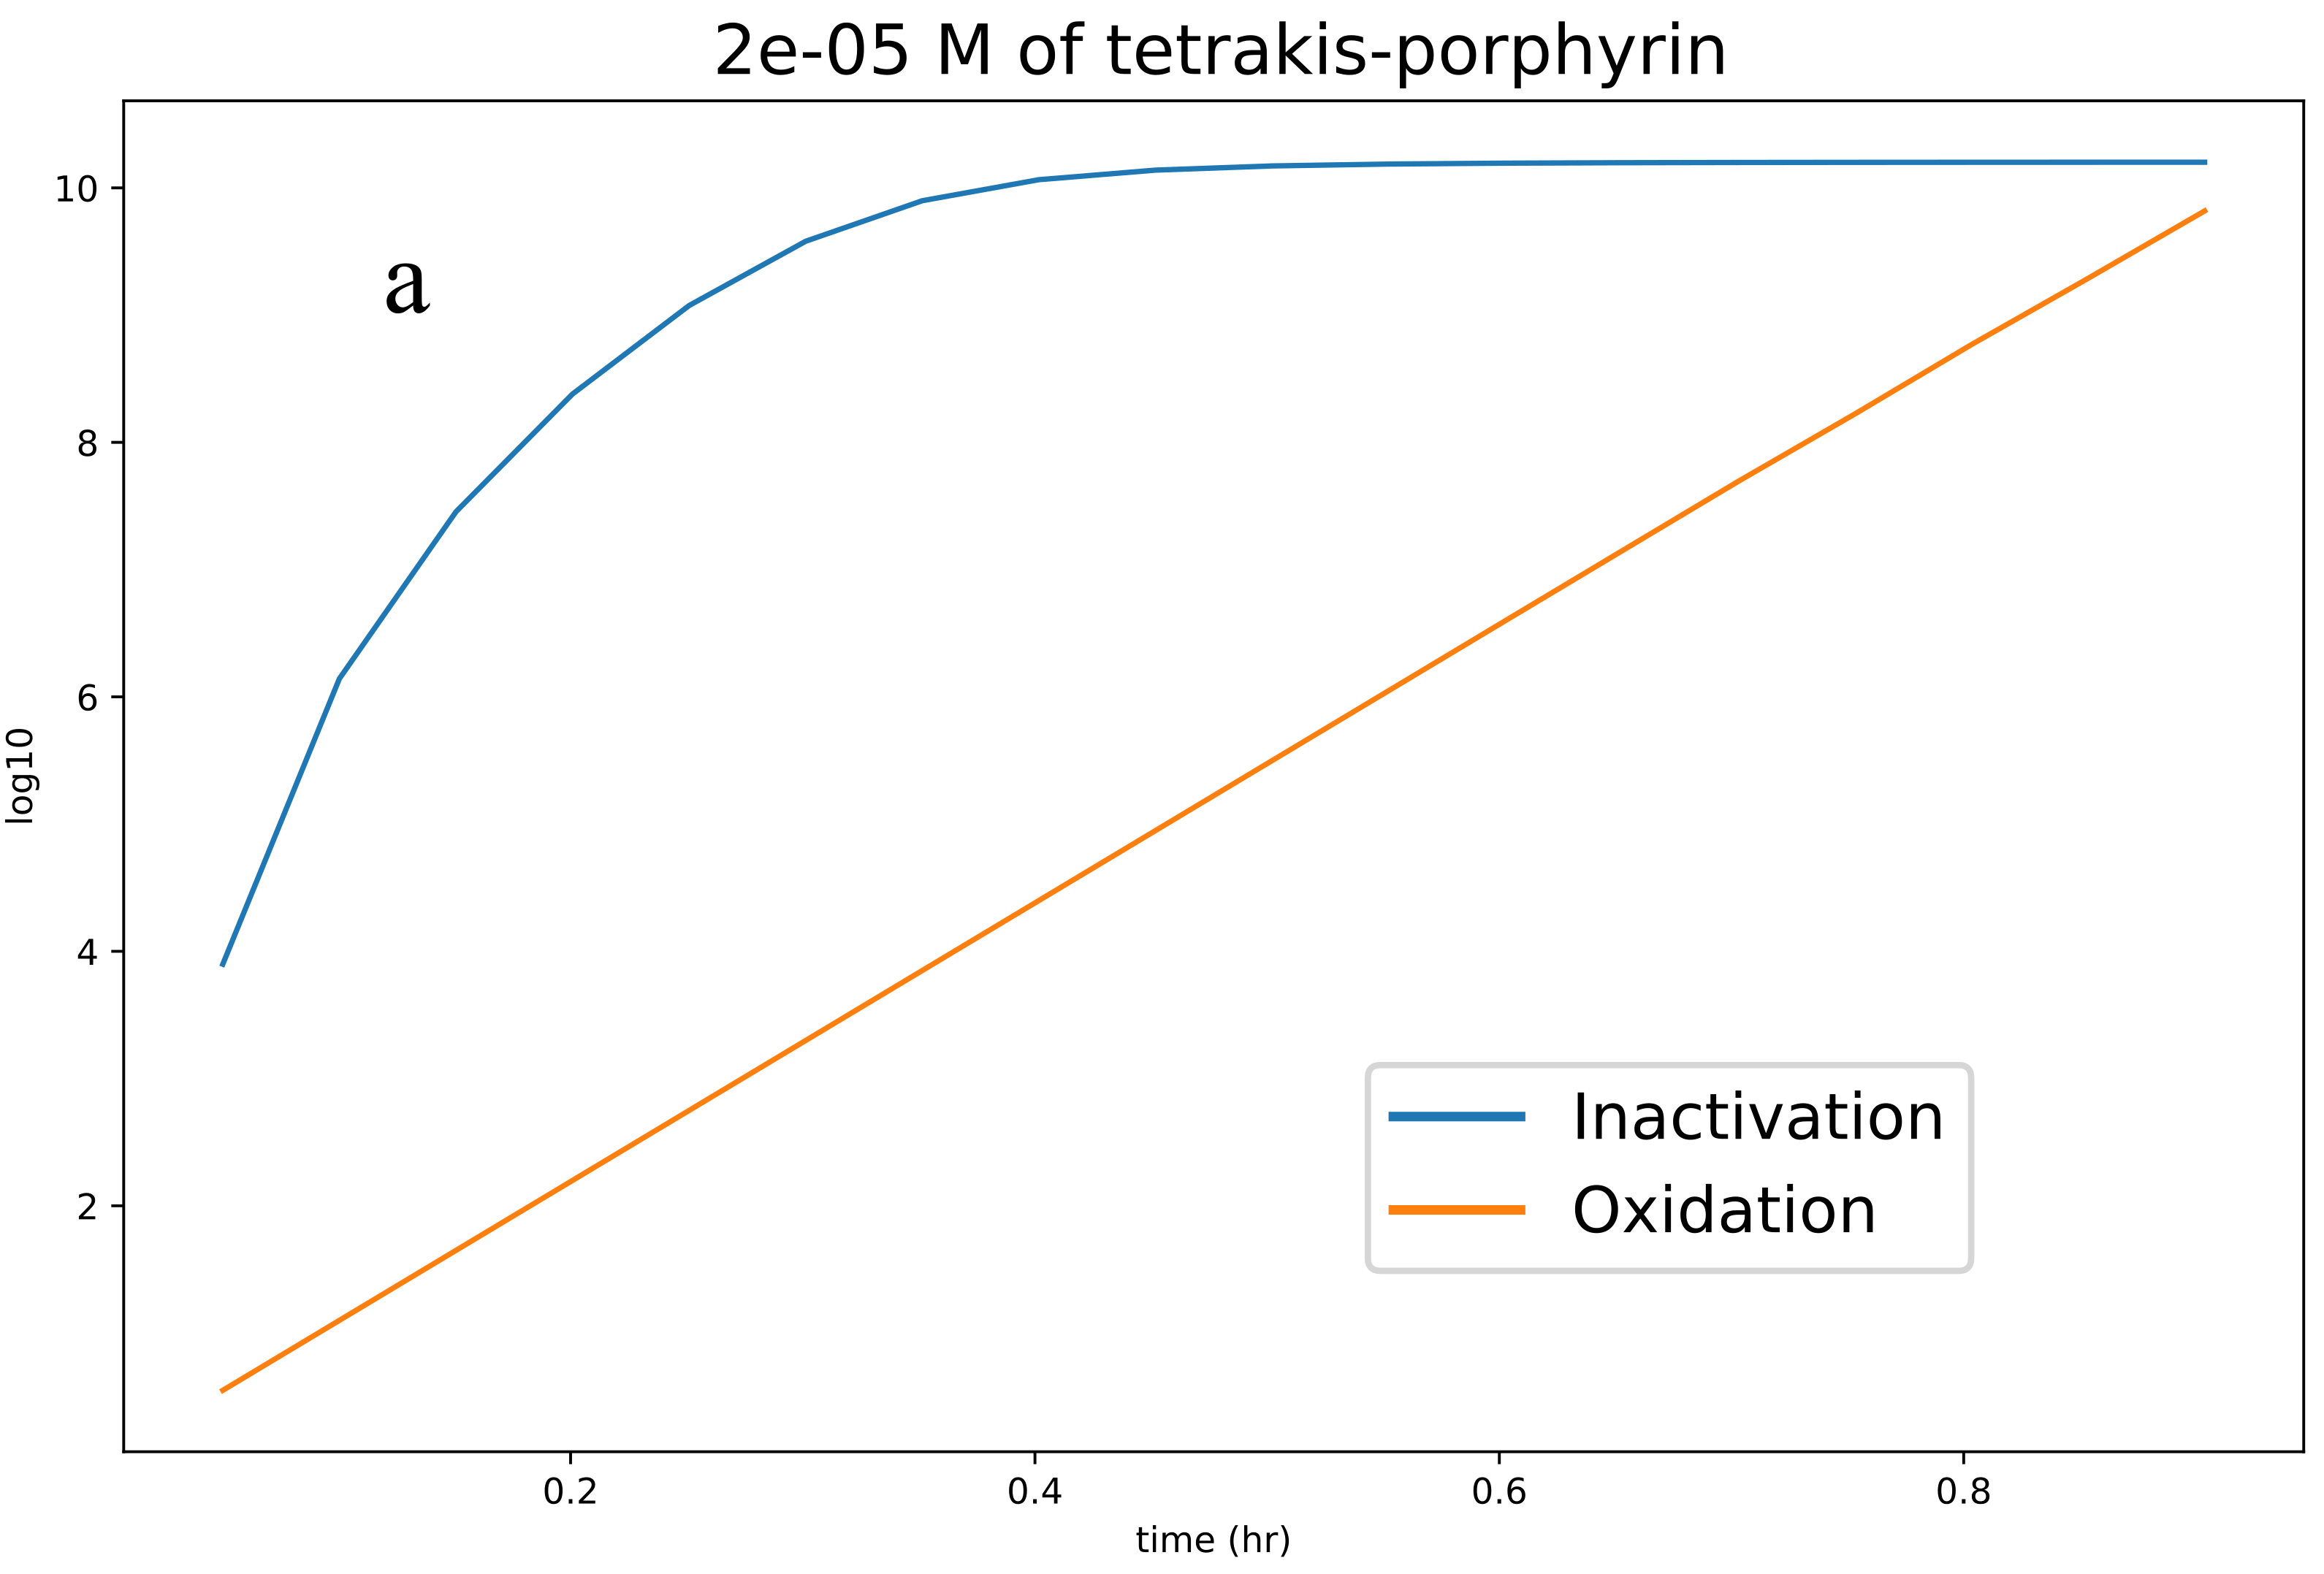
\includegraphics[width = 0.9\textwidth]{images/PDIpy/examples/20uM.png}
    \vspace{5mm}
    \midrule
    \vspace{5mm}
    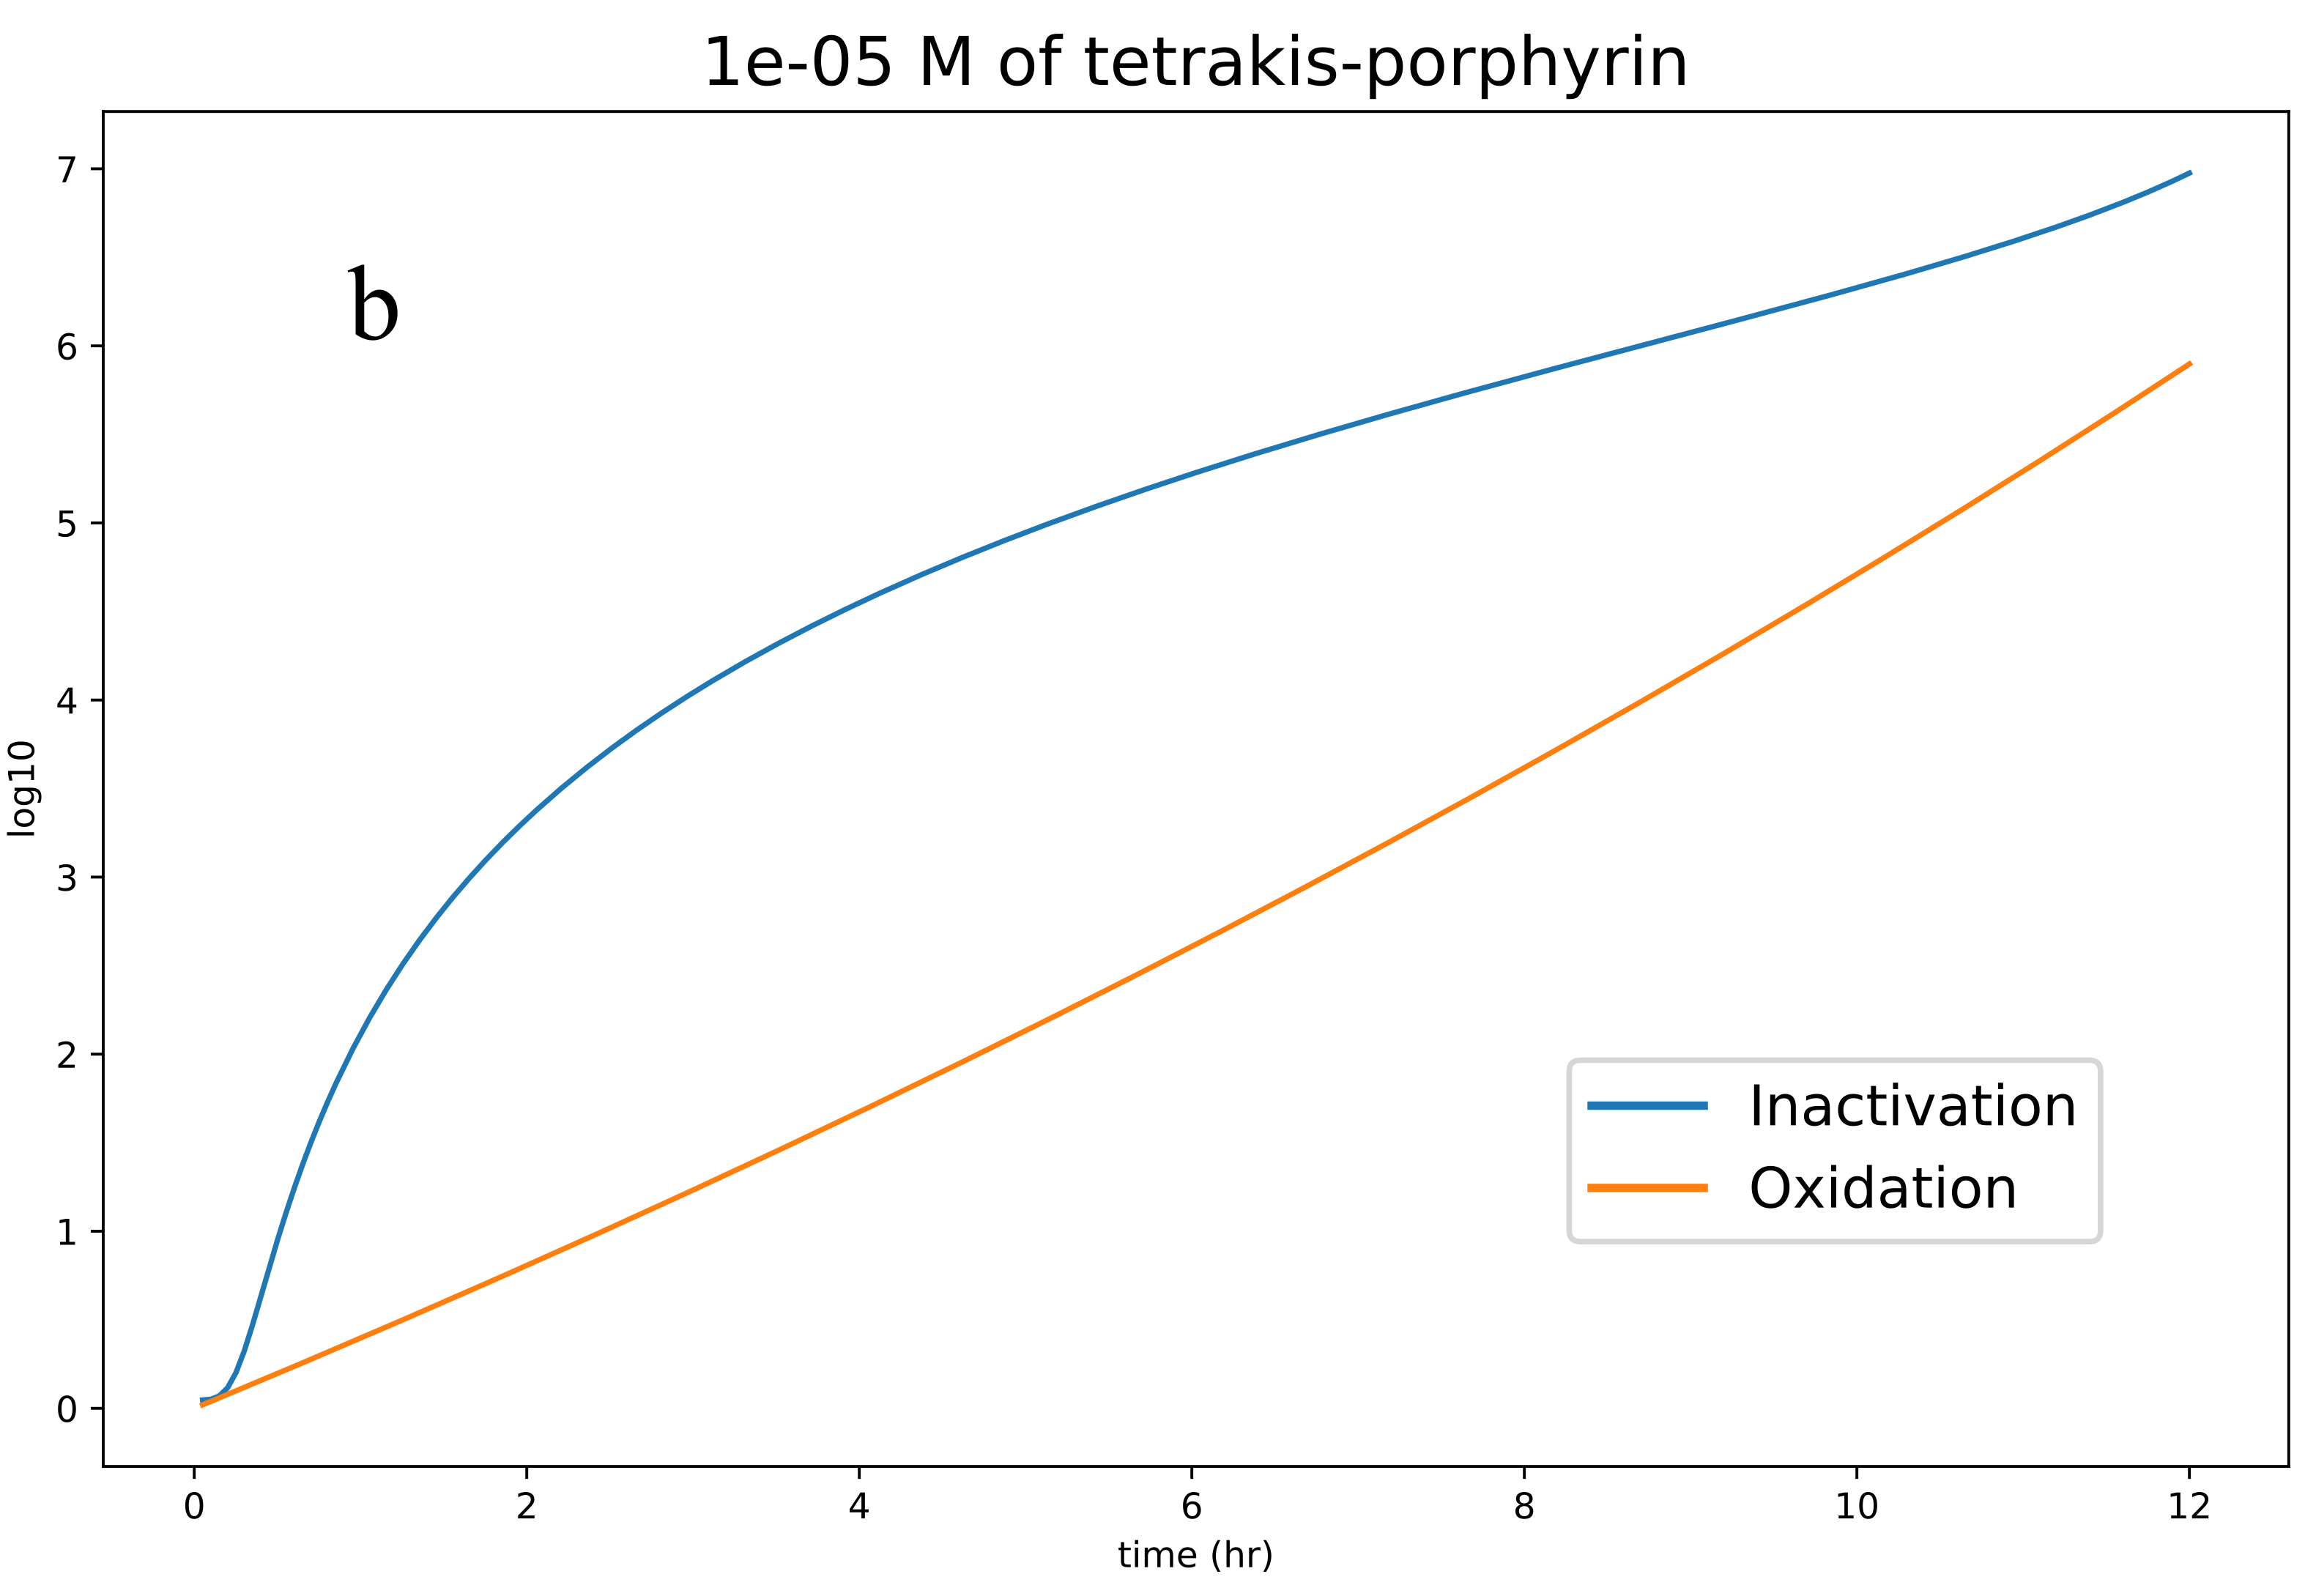
\includegraphics[width = 0.9\textwidth]{images/PDIpy/examples/10uM_biofilm.png}
    \caption{
        Two exemplary figures of PDIpy replications of the Beirao et al. data for a) planktonic and b) biofilm bacterial states.
    }
    \label{beirao_et_al}
\end{figure}

\begin{figure}
    \centering
    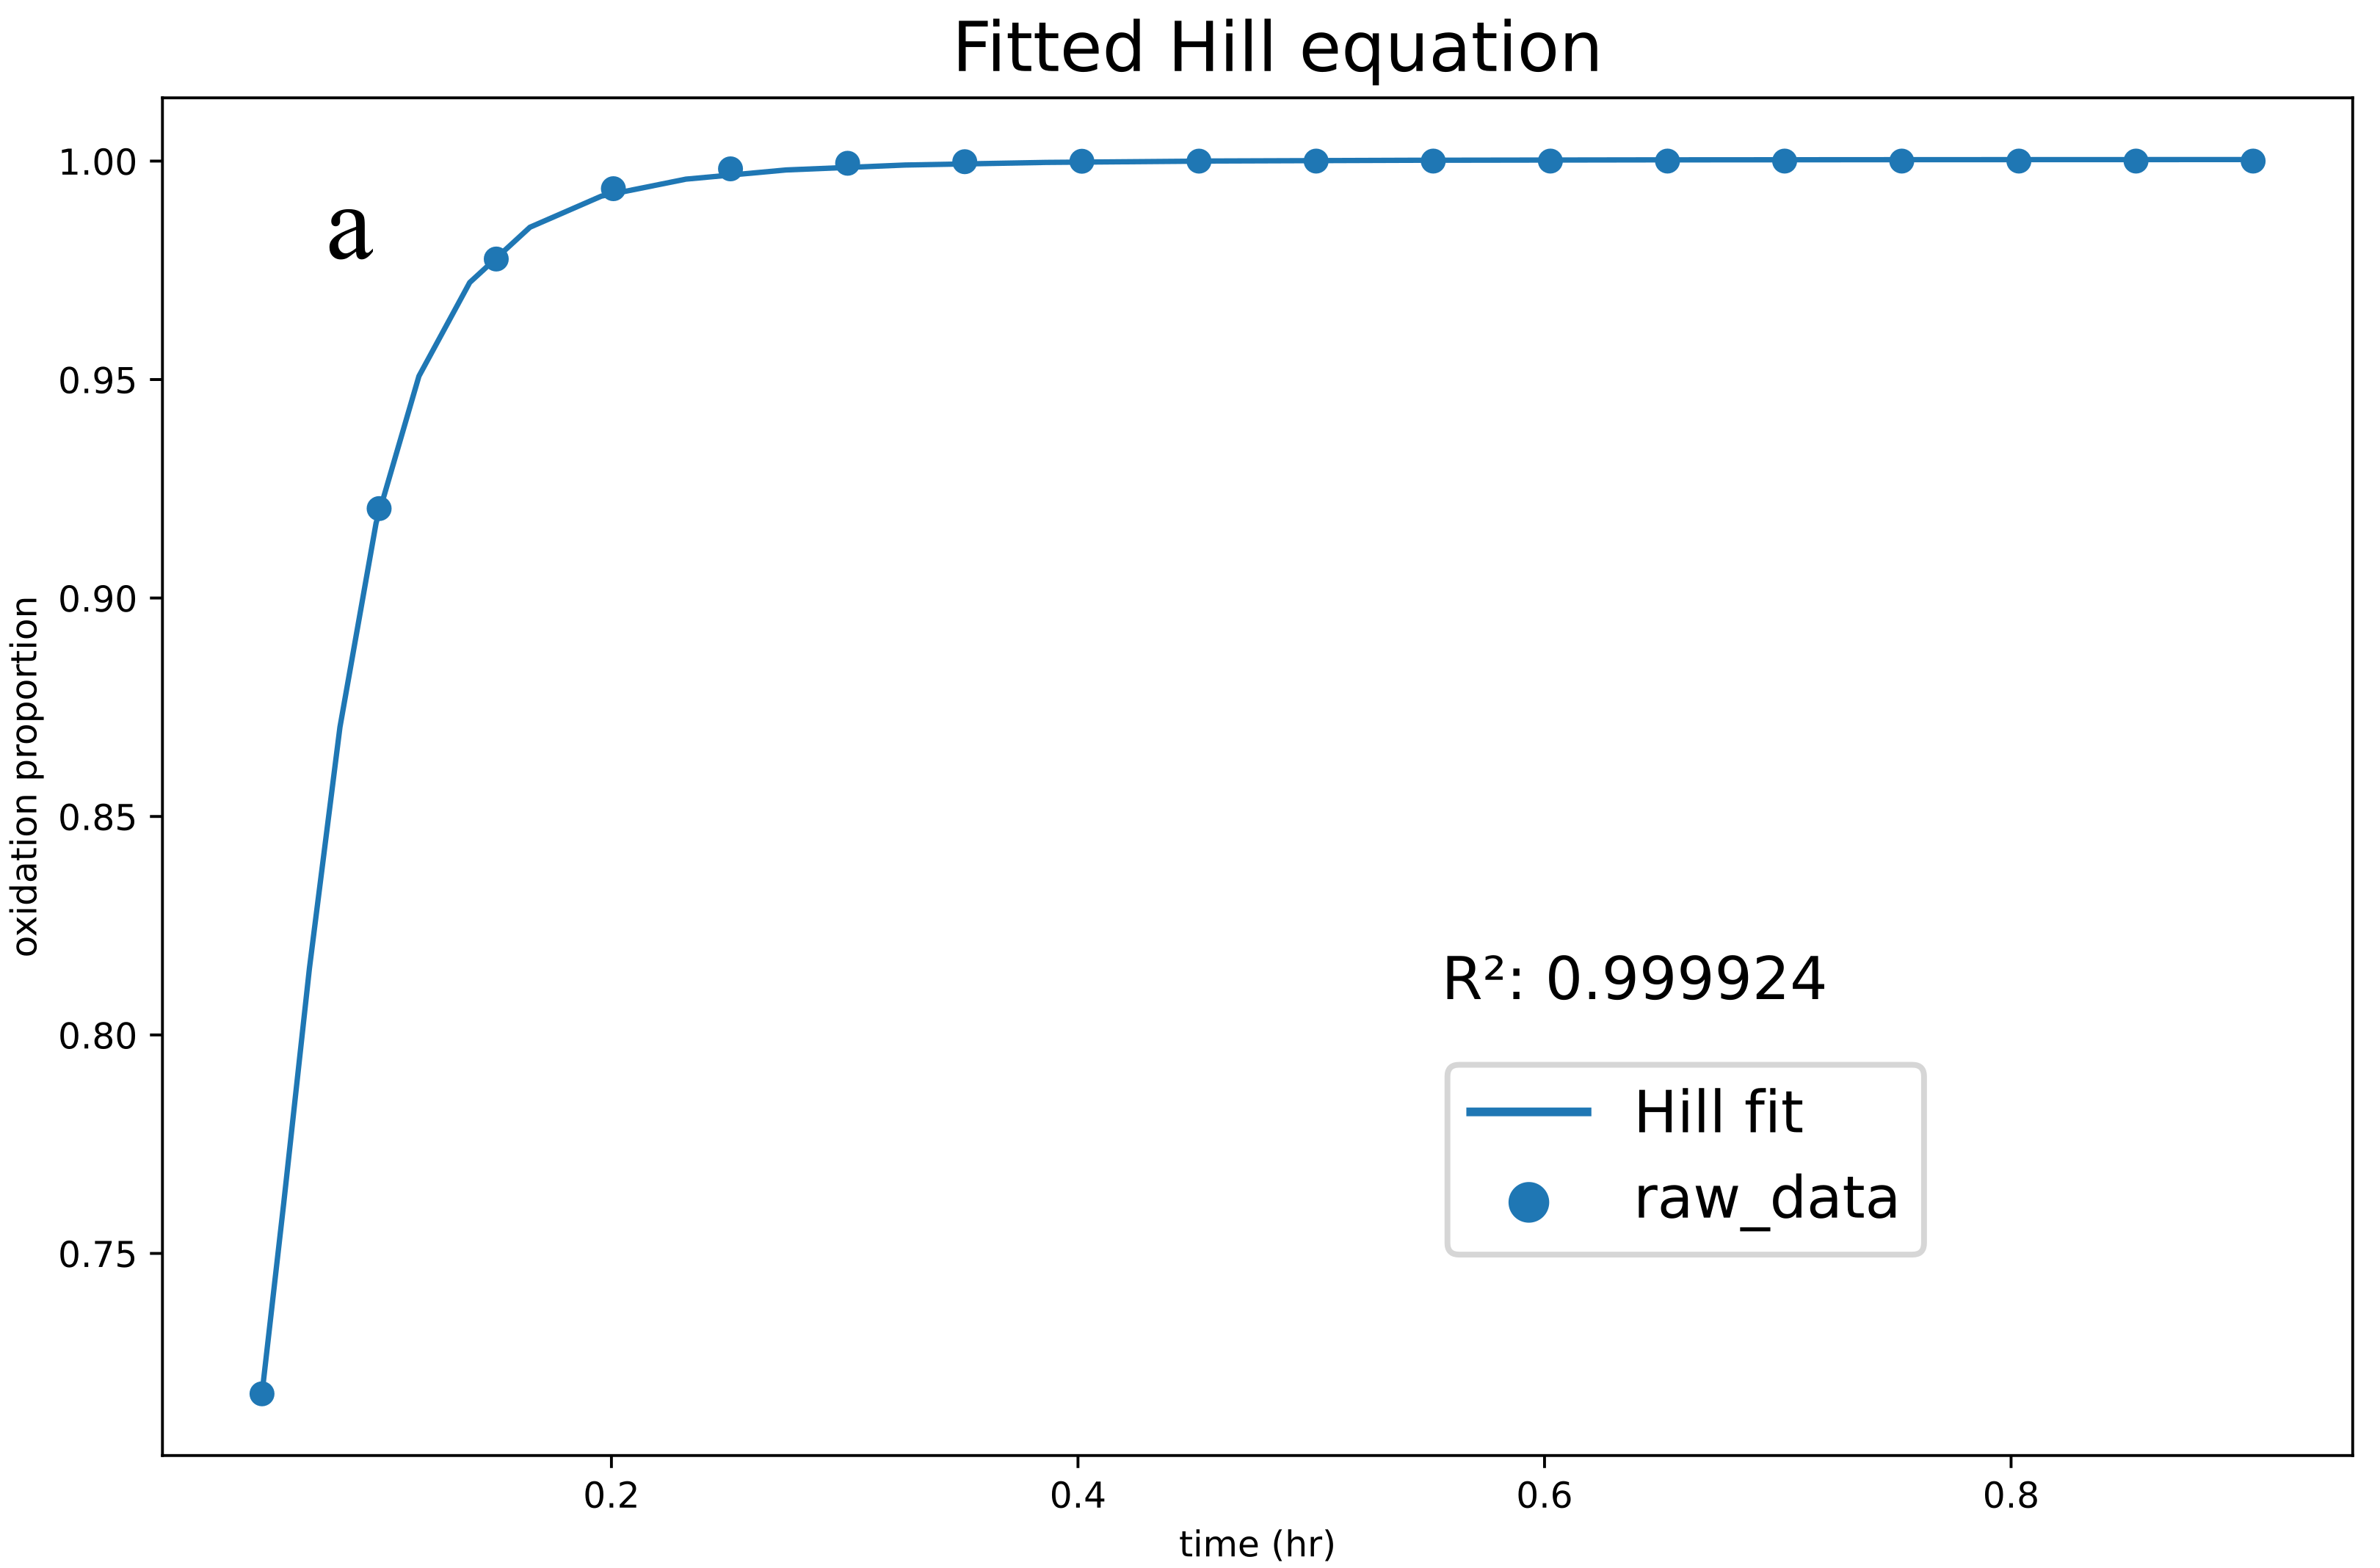
\includegraphics[width = 0.9\textwidth]{images/PDIpy/examples/20uM_regression.png}
    \vspace{5mm}
    \midrule
    \vspace{5mm}
    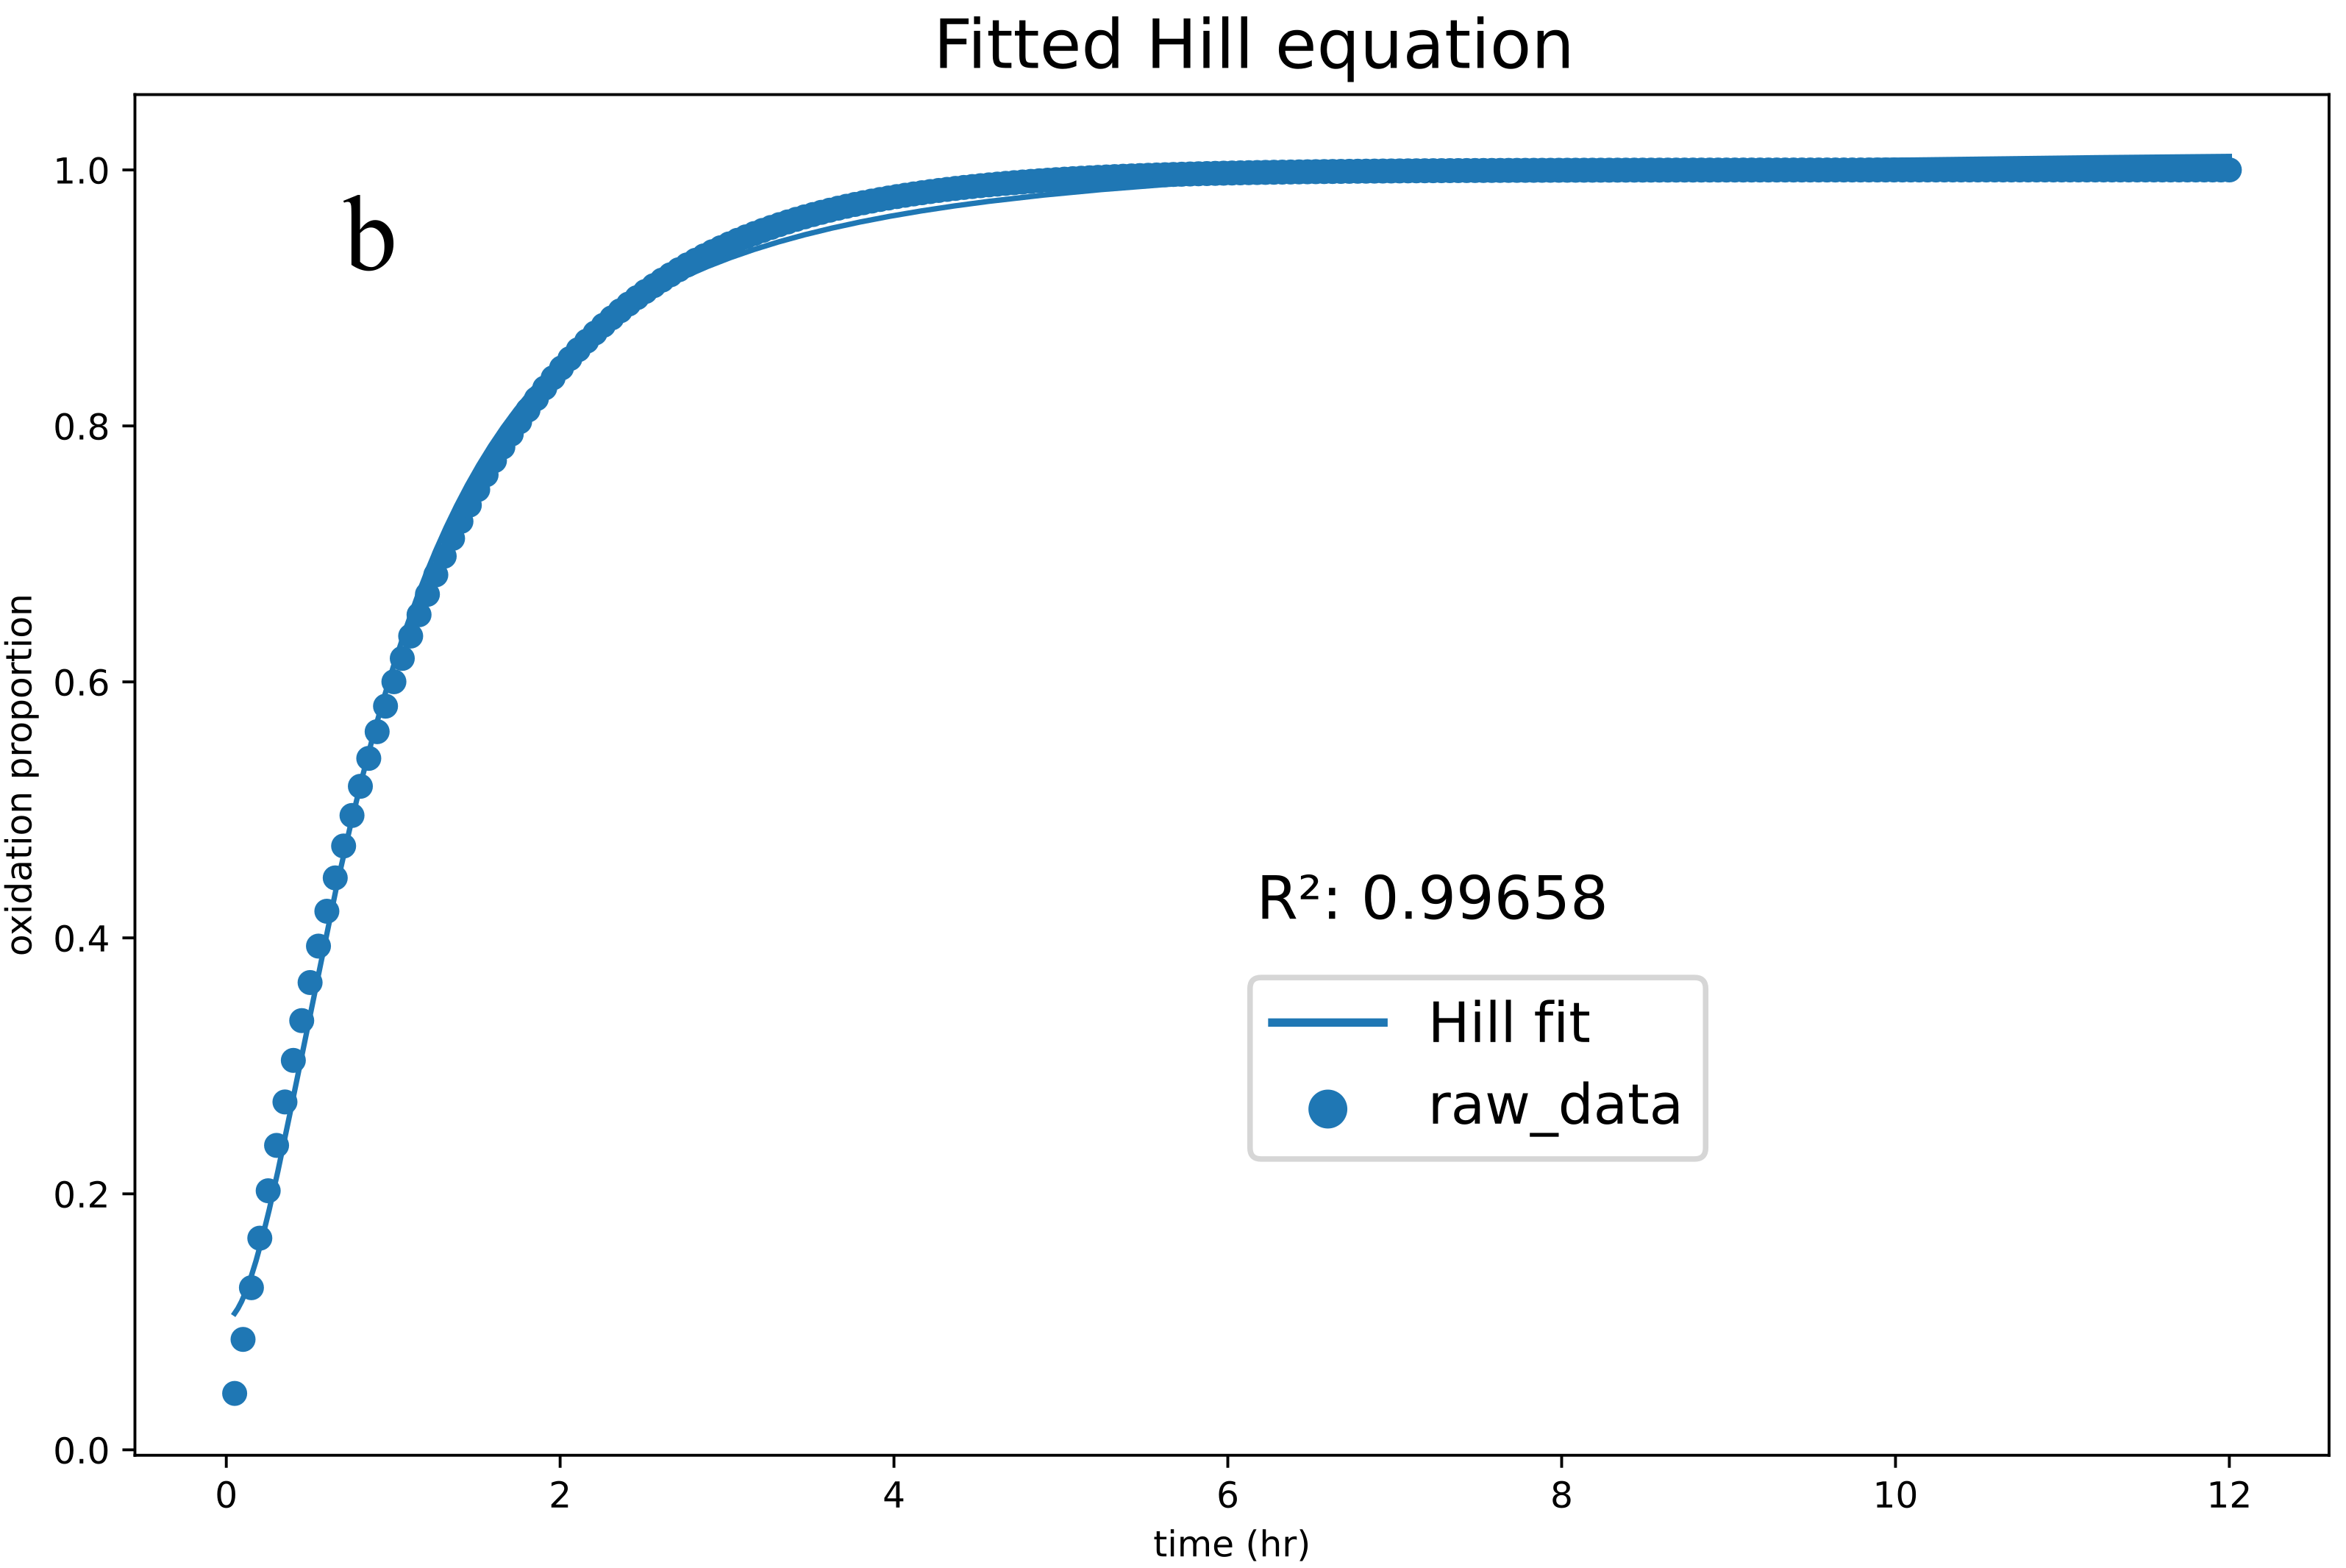
\includegraphics[width = 0.9\textwidth]{images/PDIpy/examples/10uM_biofilm_regression.png}
    \caption{
        The Hill-equation regression of the oxidation plot from Figure \ref{beirao_et_al}a. The high $R^2$ correlation supports that our chemical model of PDI is a sensible recreation of the fundamental biochemistry.
    }
    \label{hill_regression}
\end{figure}


\section{Sensitivity analyses}

\paragraph{Light intensity}
The sensitivity of simulation results to light intensities, across the range of $[10, 100,000] Lux$, was explored. The trend over this 3-log range, which is represented by Figure \ref{light_intensities}, is that the proportion of excited PS asymptotically approches 100\%. The influence of photobleaching appears to be negligible at the examined time length and light intensity, where a negative slope in the plotted excitation proportion would be expected over time as a decreasing proportion of PSs are able to electronically excite. The analysis further clarifies the minmal value of greater irradiation beyond $\approx 13,000 lux$ from the perspective of exciting PSs, which may be an informative for experimentalists when designing PDI systems.

\begin{figure}
    \centering
    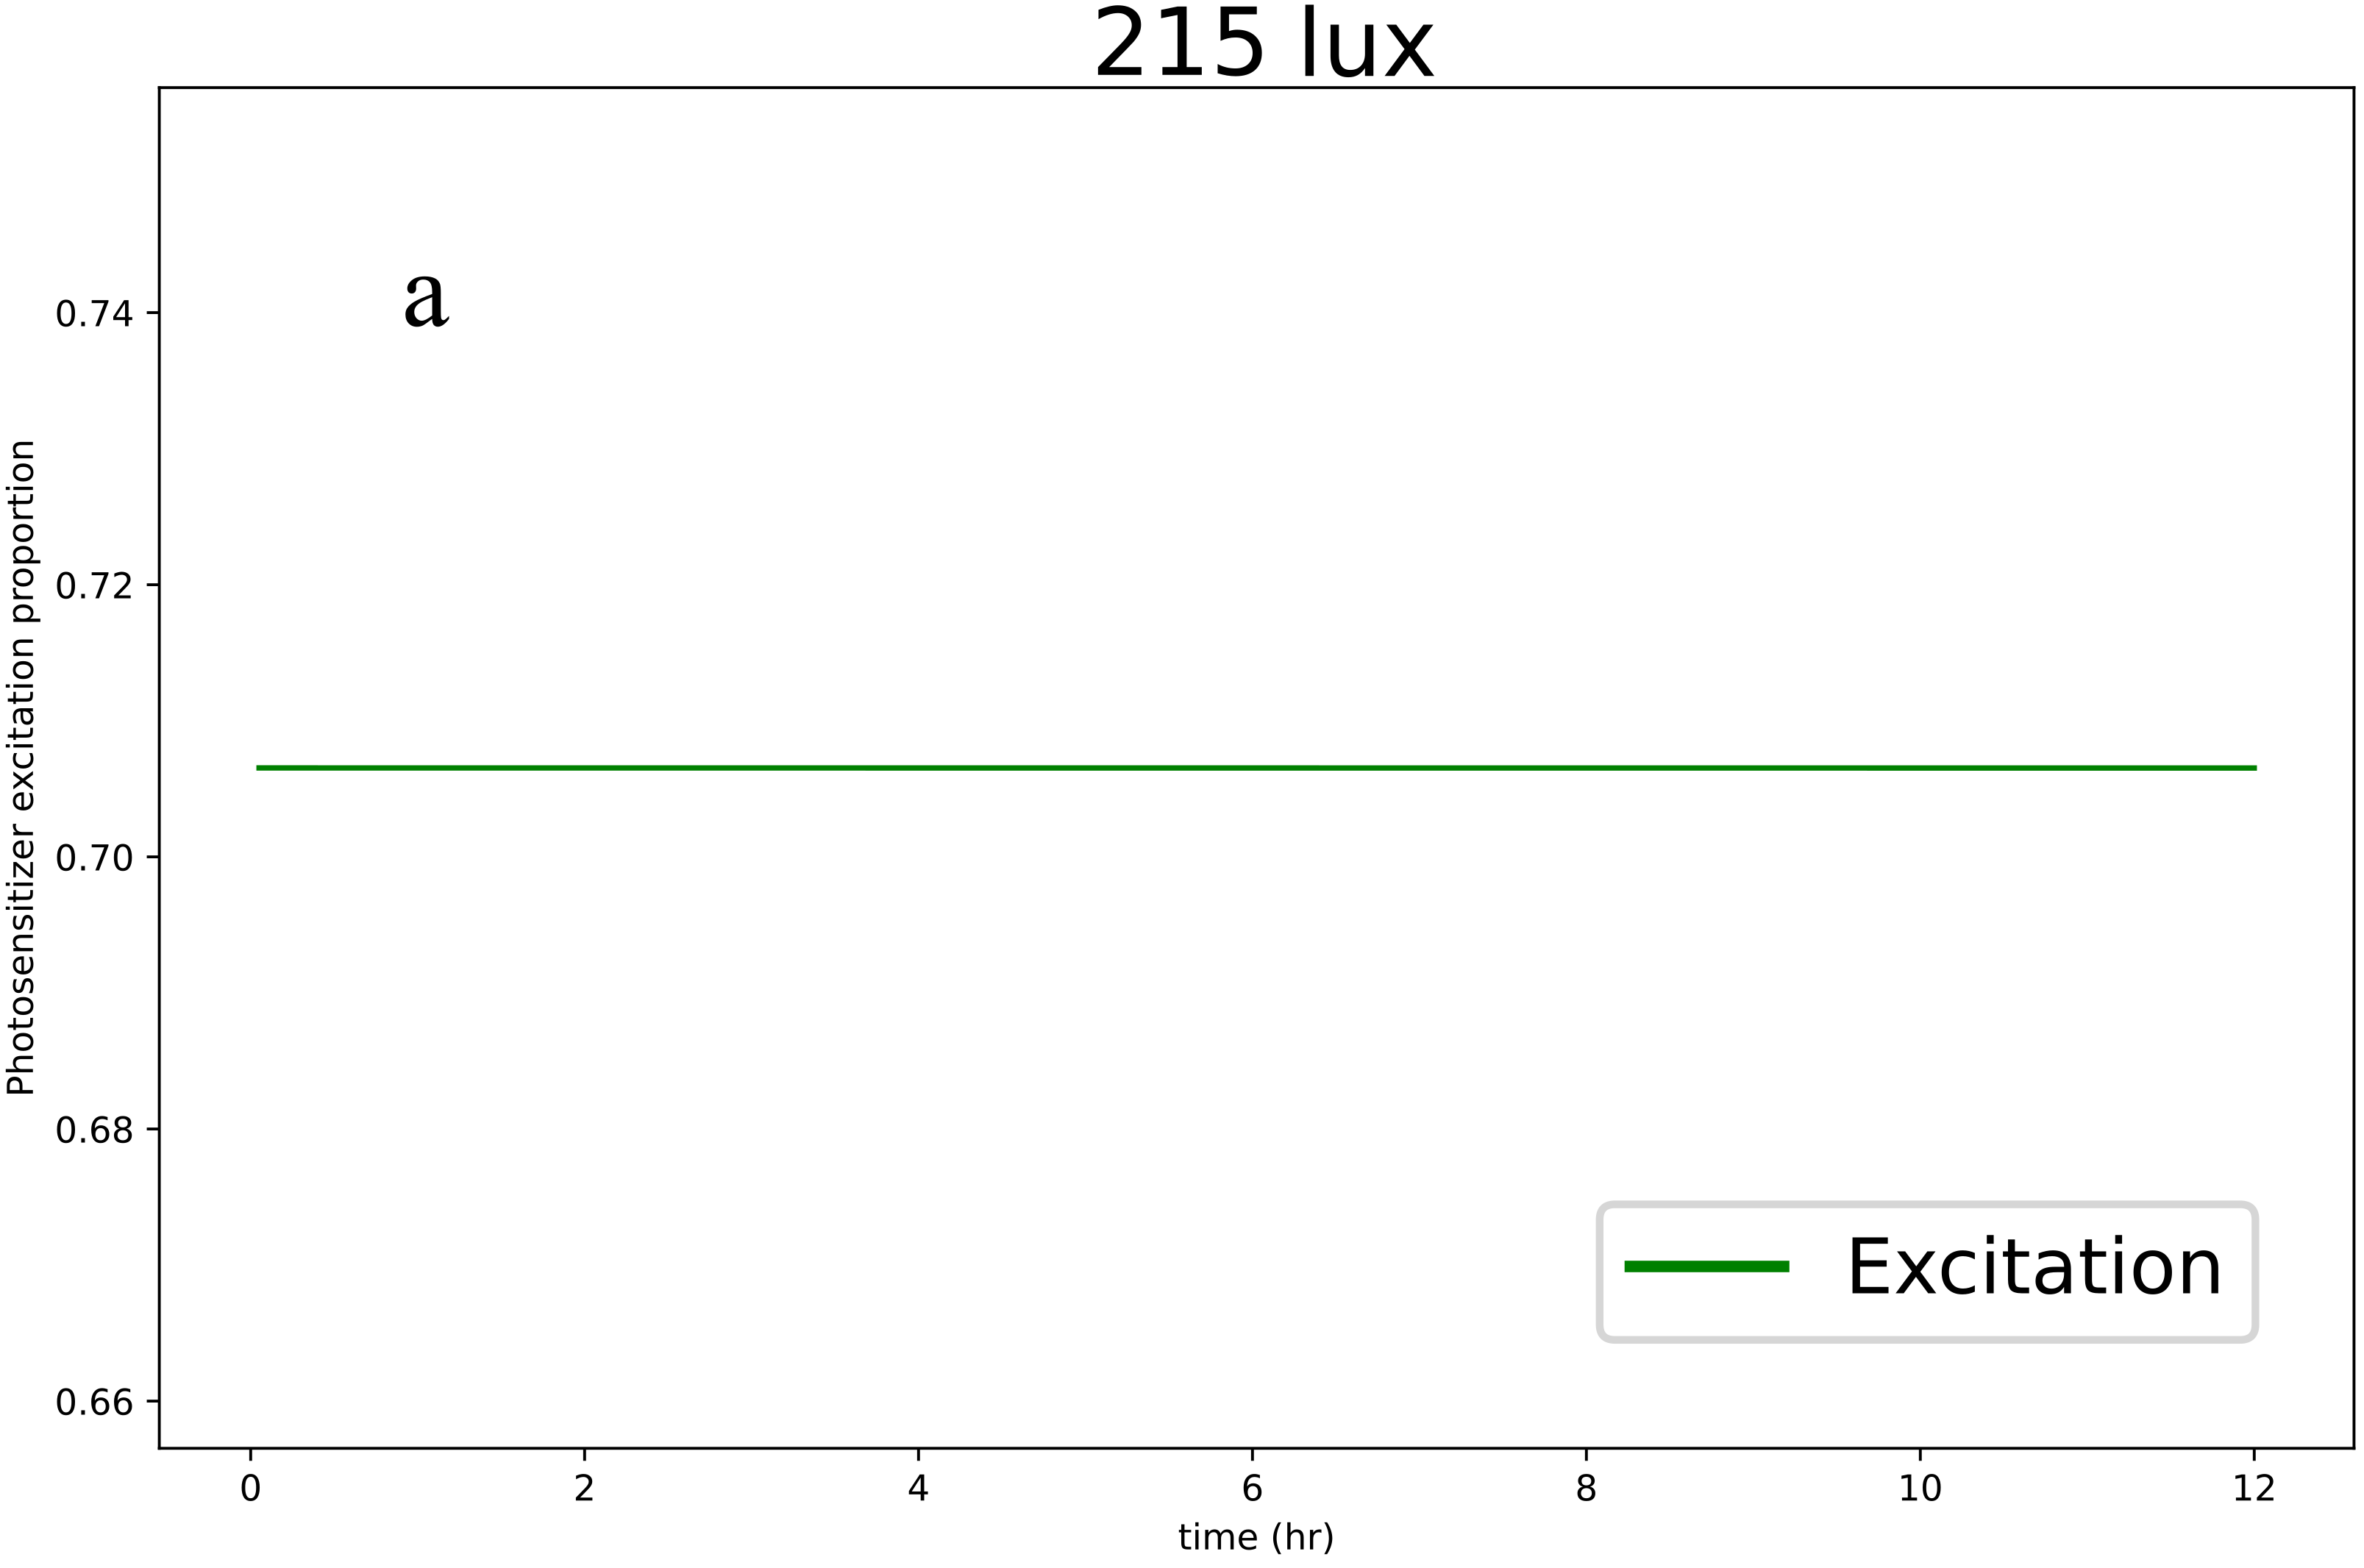
\includegraphics[width = 0.8\textwidth]{images/PDIpy/sensitivity_analyses/215_lux.png} \\
    \vspace{5mm}
    \midrule
    \vspace{5mm}
    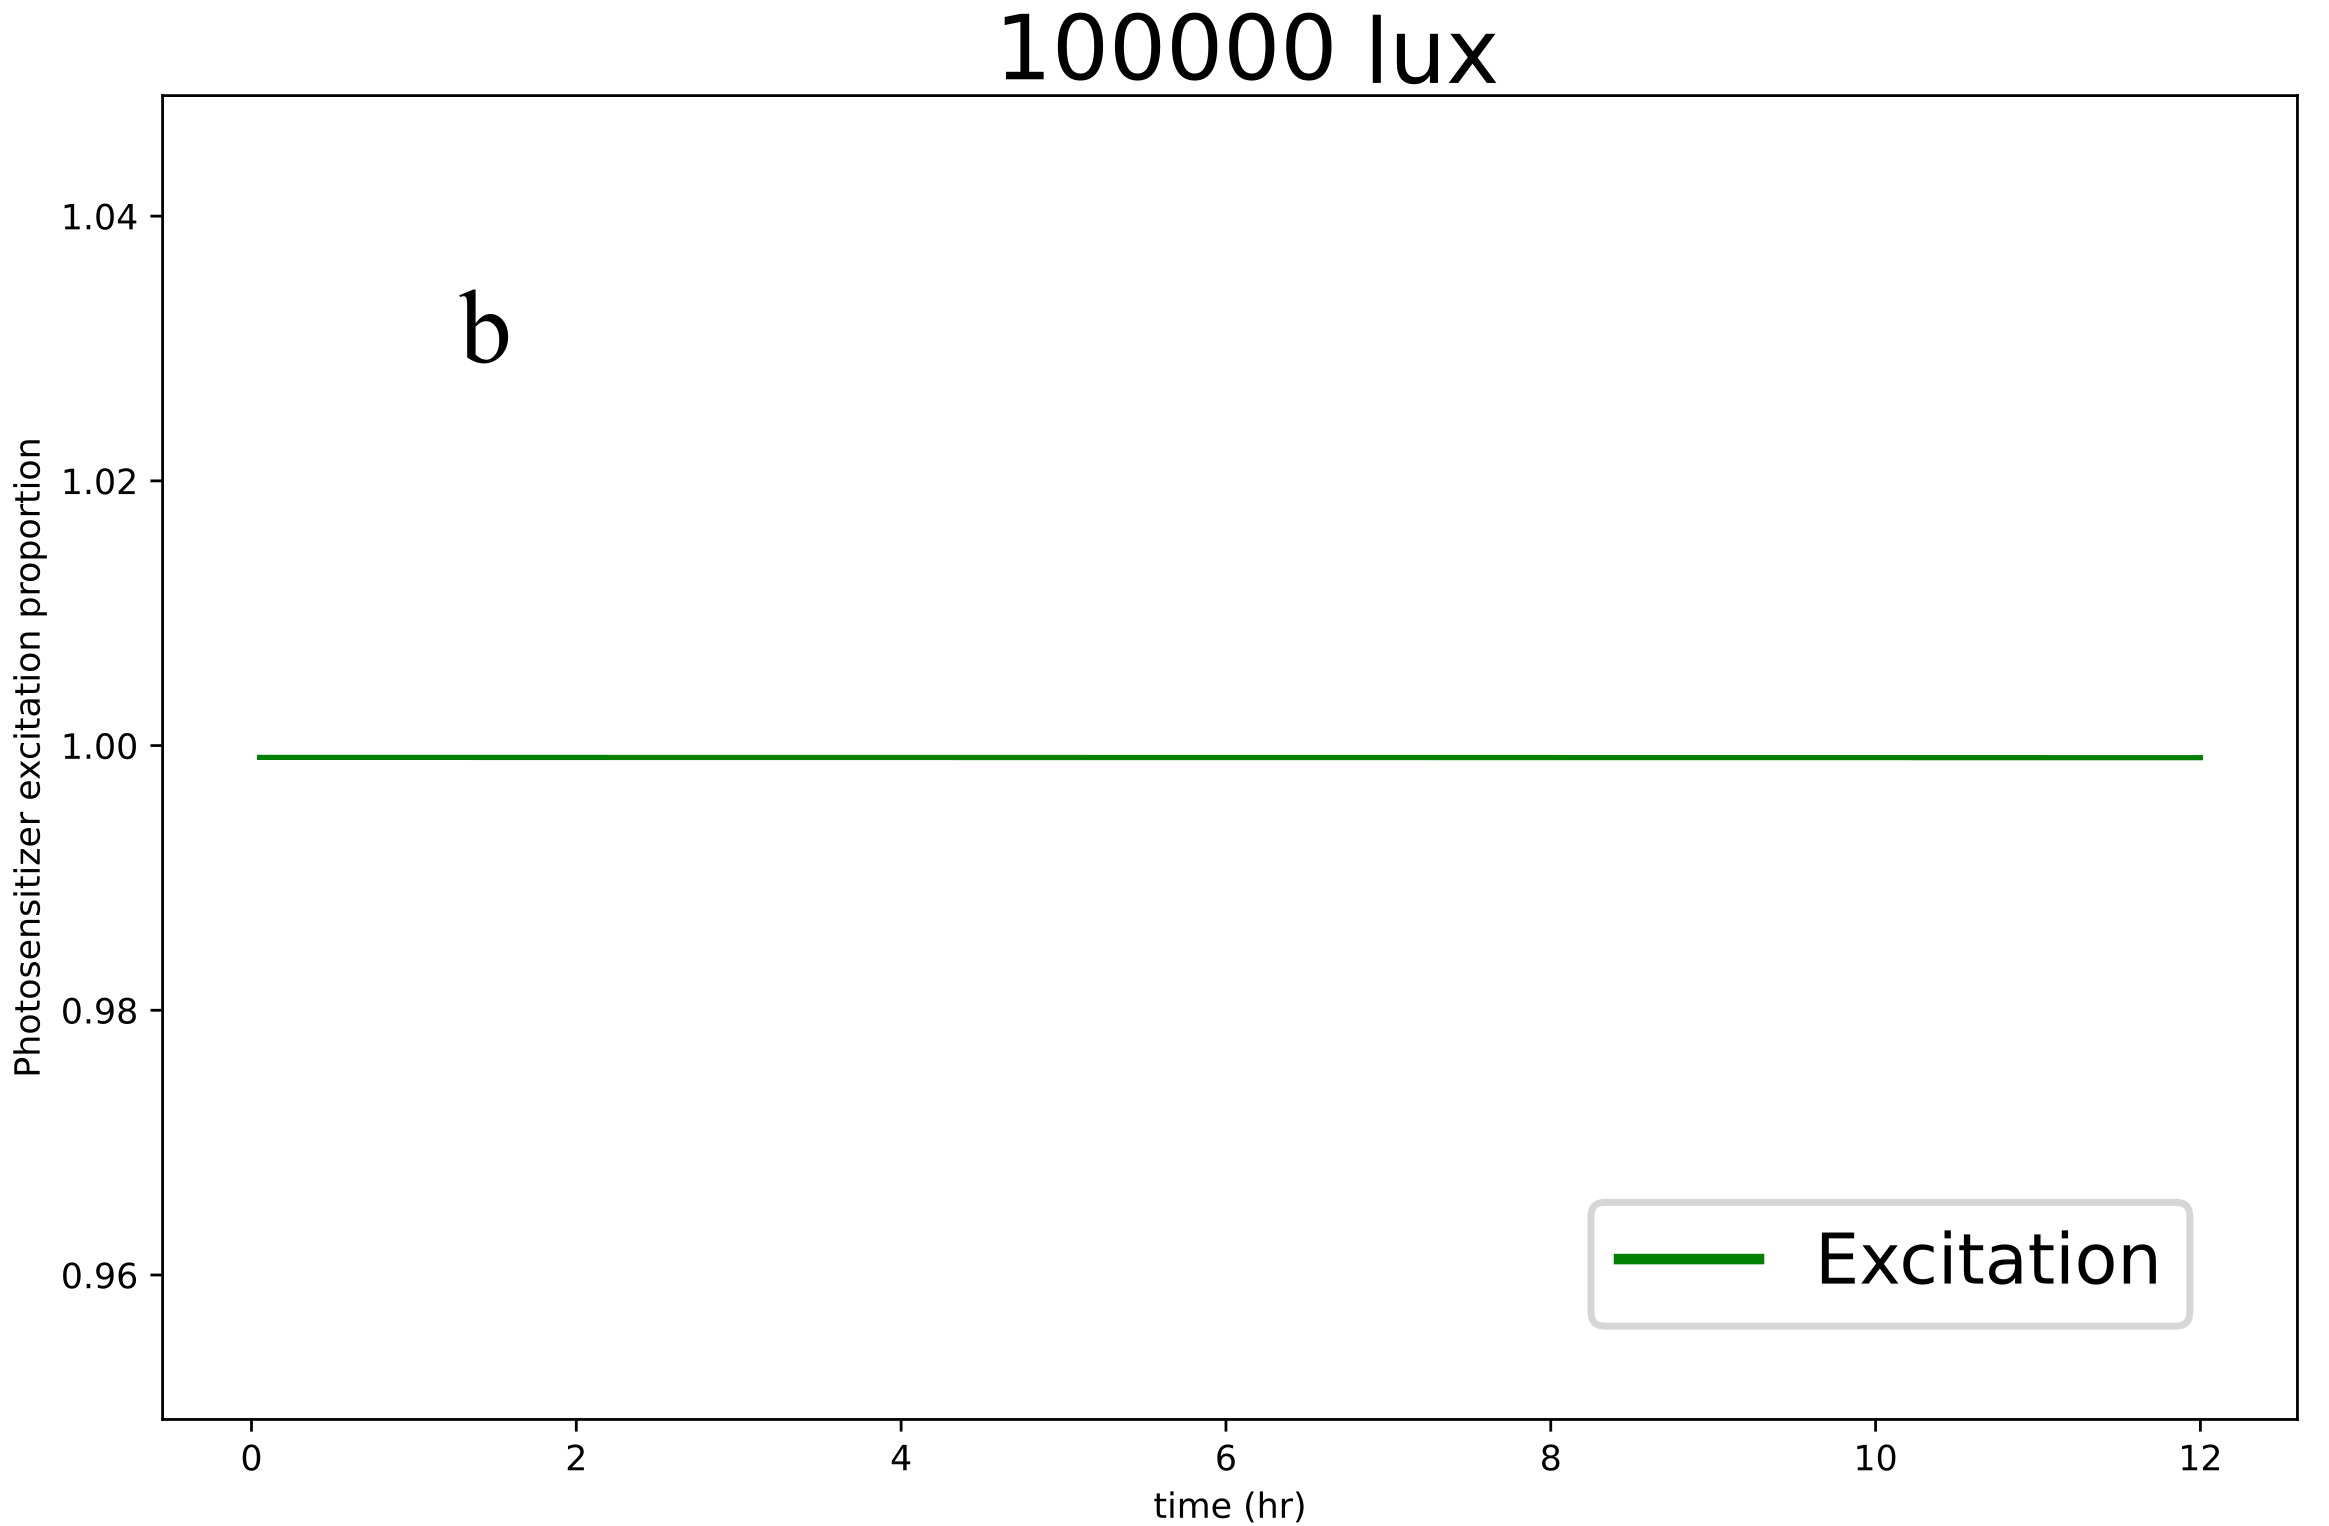
\includegraphics[width = 0.8\textwidth]{images/PDIpy/sensitivity_analyses/100000_lux.png}
    \caption{
        The proportion of excited PS at two contrasting light intensities: a) $215 Lux$ and b) $100000 Lux$. The negative slope of the plots is the consequence of photobleaching, where the quantity of excitable PSs decreases over time. This effect is more prominent in b) since the light intensity is much greater than a), and since photobleaching is a function of light intensity.
    }
    \label{light_intensities}
\end{figure}

\section{Discussion}
The preliminary examples of PDIpy with the study from Beirao et al. support that the underlying kinetic model sufficiently represents PDI. The excessive breadth in the simulation predictions, where the log-inactivation predictions with low concentrations occurs too late while the log-inactivation predictions with high concentrations occurs too early, may be resolved with adjusted the Hill parameters that are defined in Table \ref{hill_parameters}. The tighter spread of the biofilm simulation relative to the planktonic simulation supports this method of improving the predicted results, where the different set of parameter adjustments may be better tailored to inactivation phenomena. 

The sensitivity analysis of the light intensity revealed that the relationship between the proportion of PS excitation and the light intensity plateaus beyond $\approx 10,000 lux$. This insight and this type of broad inquiry over a range of values cannot be replicated with existing PDI models, since they neither consider the fundamental kinetics that results in PS excitation nor are encapsulated in a dynamic interface like the PDIpy API.  

The open-source implementation of this model in PDIpy will practically support experimentalists as they develop PDI technologies, and will ideally inspire other computational biologists to develop programs that can foster discovery of antibiotic methods at an imperative time to prevent antimicrobial resistant epedemics.   


\section{Author Contributions}
\begin{description}
    \item[APF] Designed, executed, and codified the project.
    \item[JRK] Guidance and manuscript edits.
    \item[HLB] Guidance, manuscript edits, and funding.
\end{description}

\section{Acknowledgments}

The authors are grateful to Ethan Sean Chan for his development of the framework for iPDIpy, which will be introduced in a future release of PDIpy. The authors thank the members of the Buckley and Wolff Groups at the University of Victoria for contributing ideas and data that were used to refine this PDI model. Andrew finally thanks Hiroaki Imoto for his contributions and guidance in developing the HillFit module that was used to fit data in PDIpy.
\newpage
\subsection{Supporting Information: PDIpy}

\subsection{Molecular properties and mechanisms}
The electronic difference between $^1\Delta_g$ and $^3\Sigma_g^-$ is best depicted through their respective molecular orbital diagrams in Figure \ref{mo_diagrams}. The photochemical processes of $^1\Delta_g$ generation are depicted in Figure \ref{jablonski_diagram}, while the subsequent oxidation reactions are sampled in Figure \ref{schenck_mechanism}.

\begin{figure}
    \centering
    \begin{tabular}{c|c}
        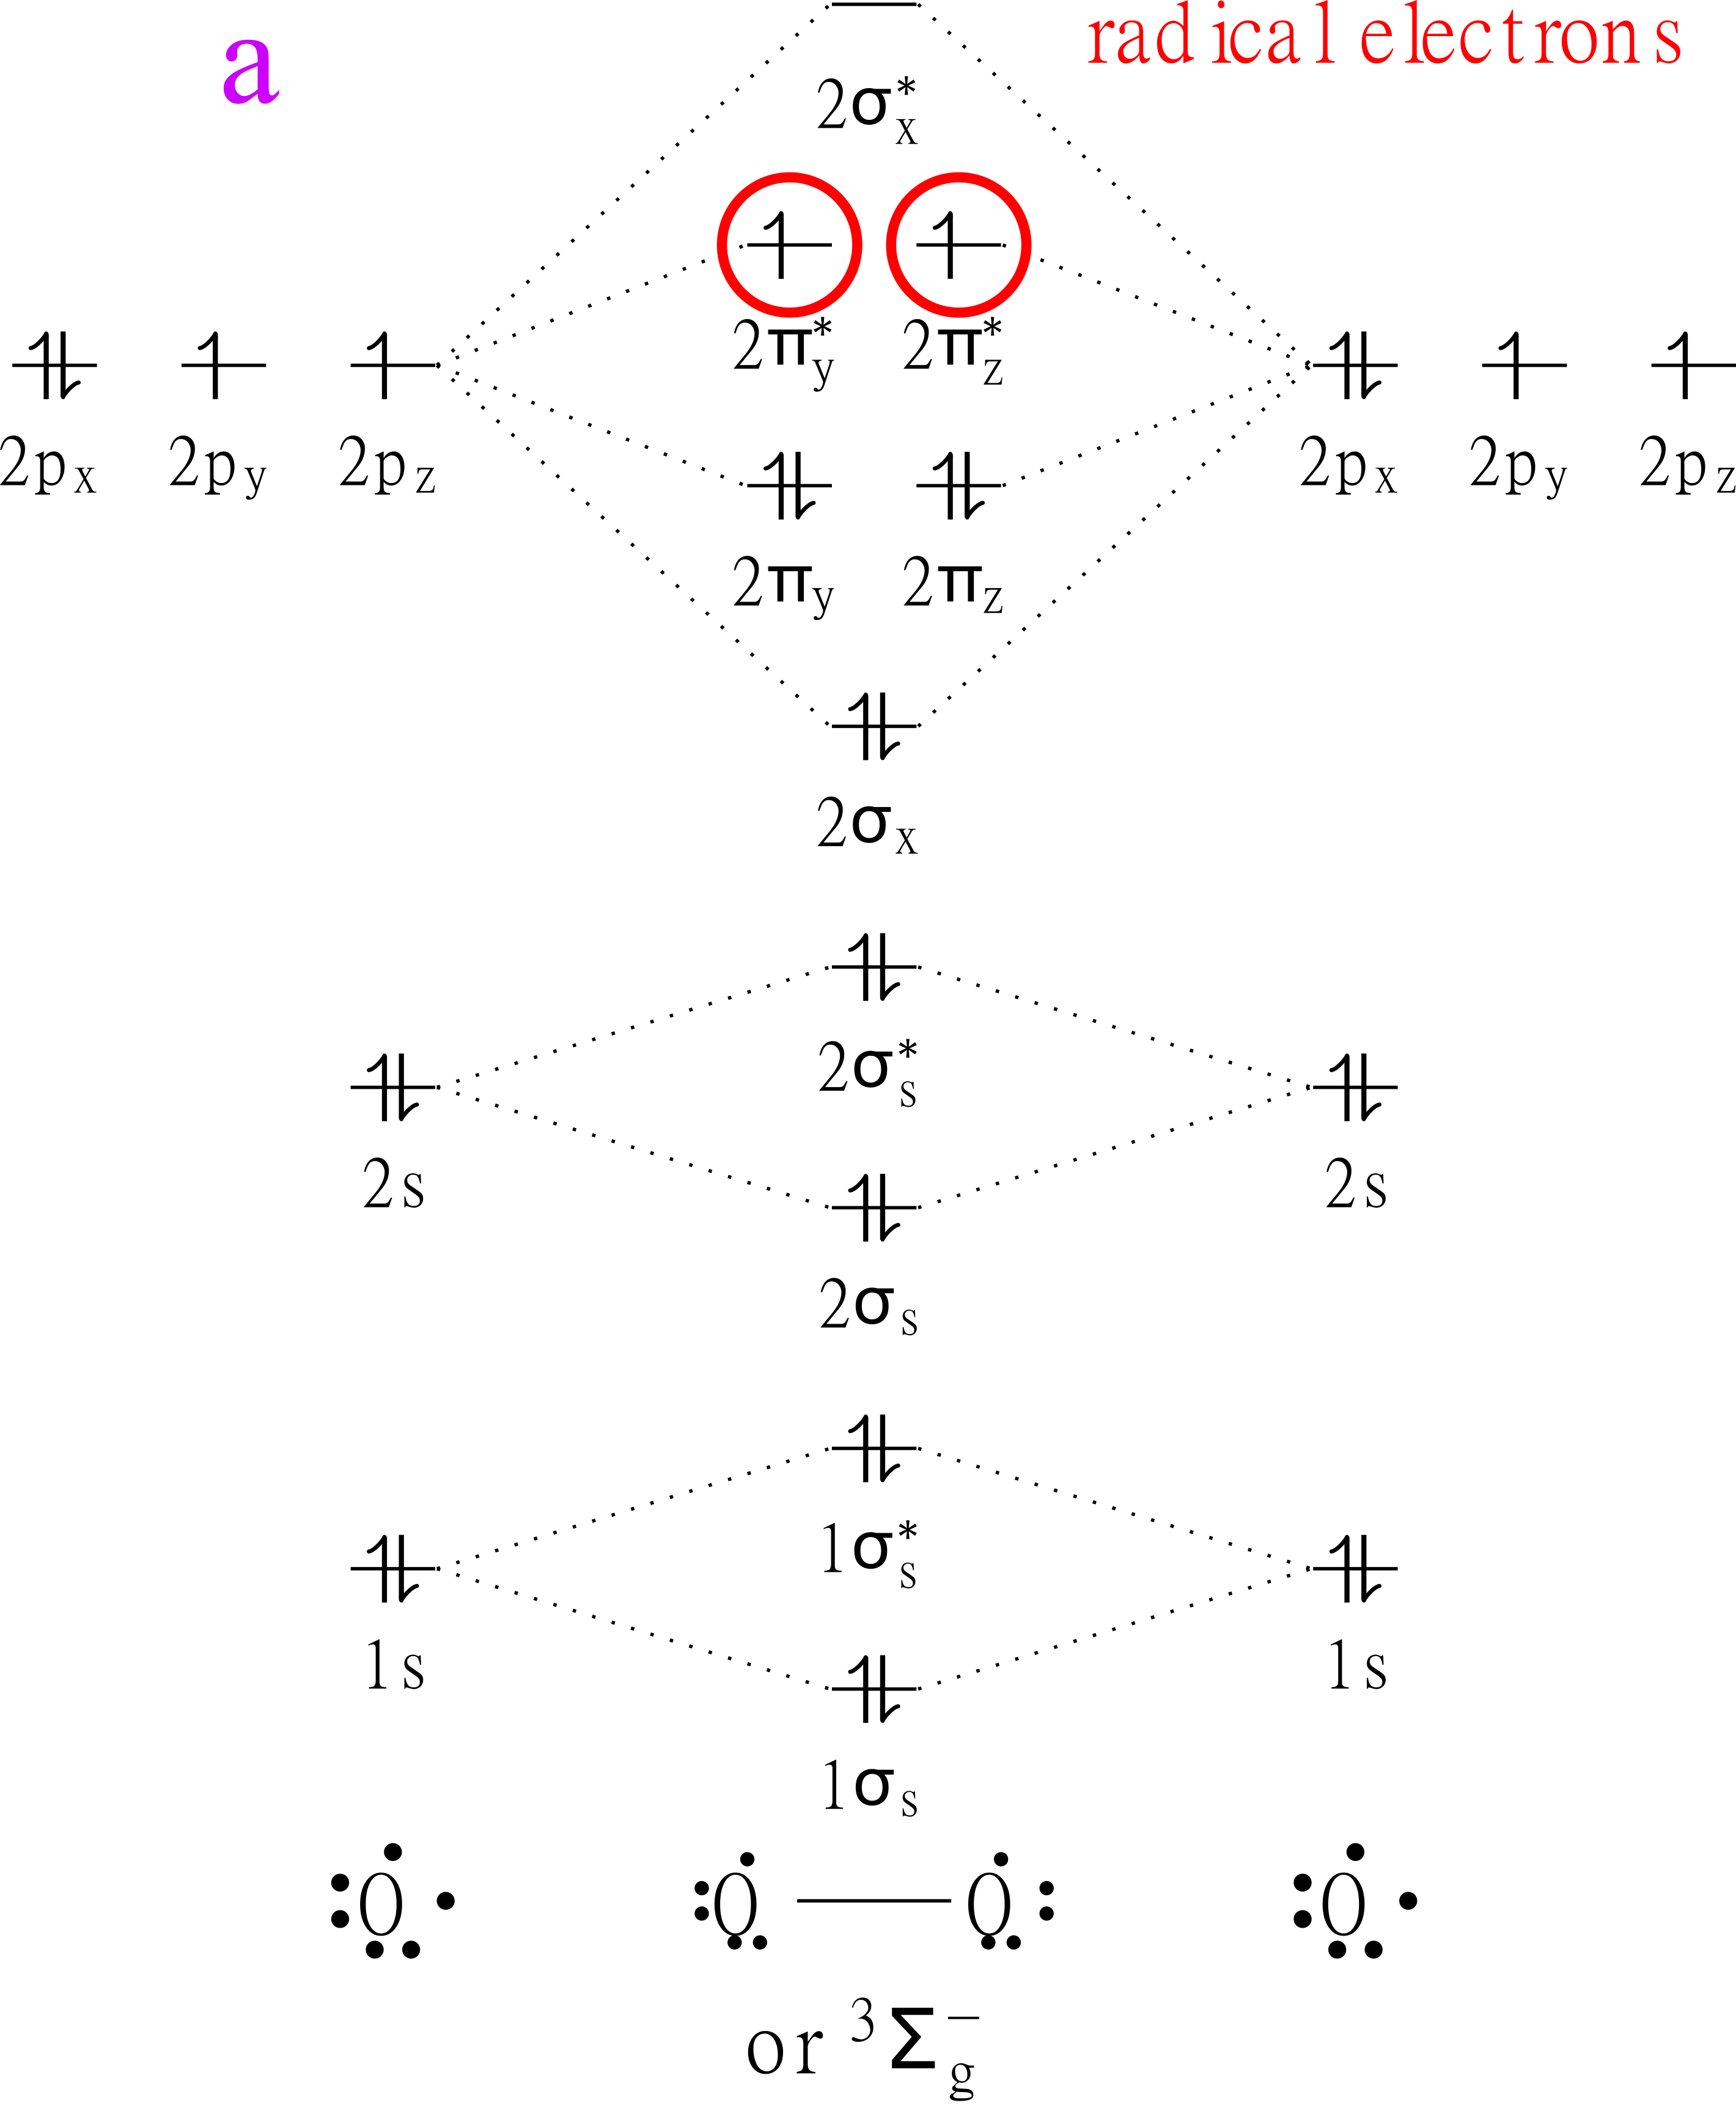
\includegraphics[width = 0.48\textwidth]{images/PDIpy/background/triplet_mo_diagram.png}
        & 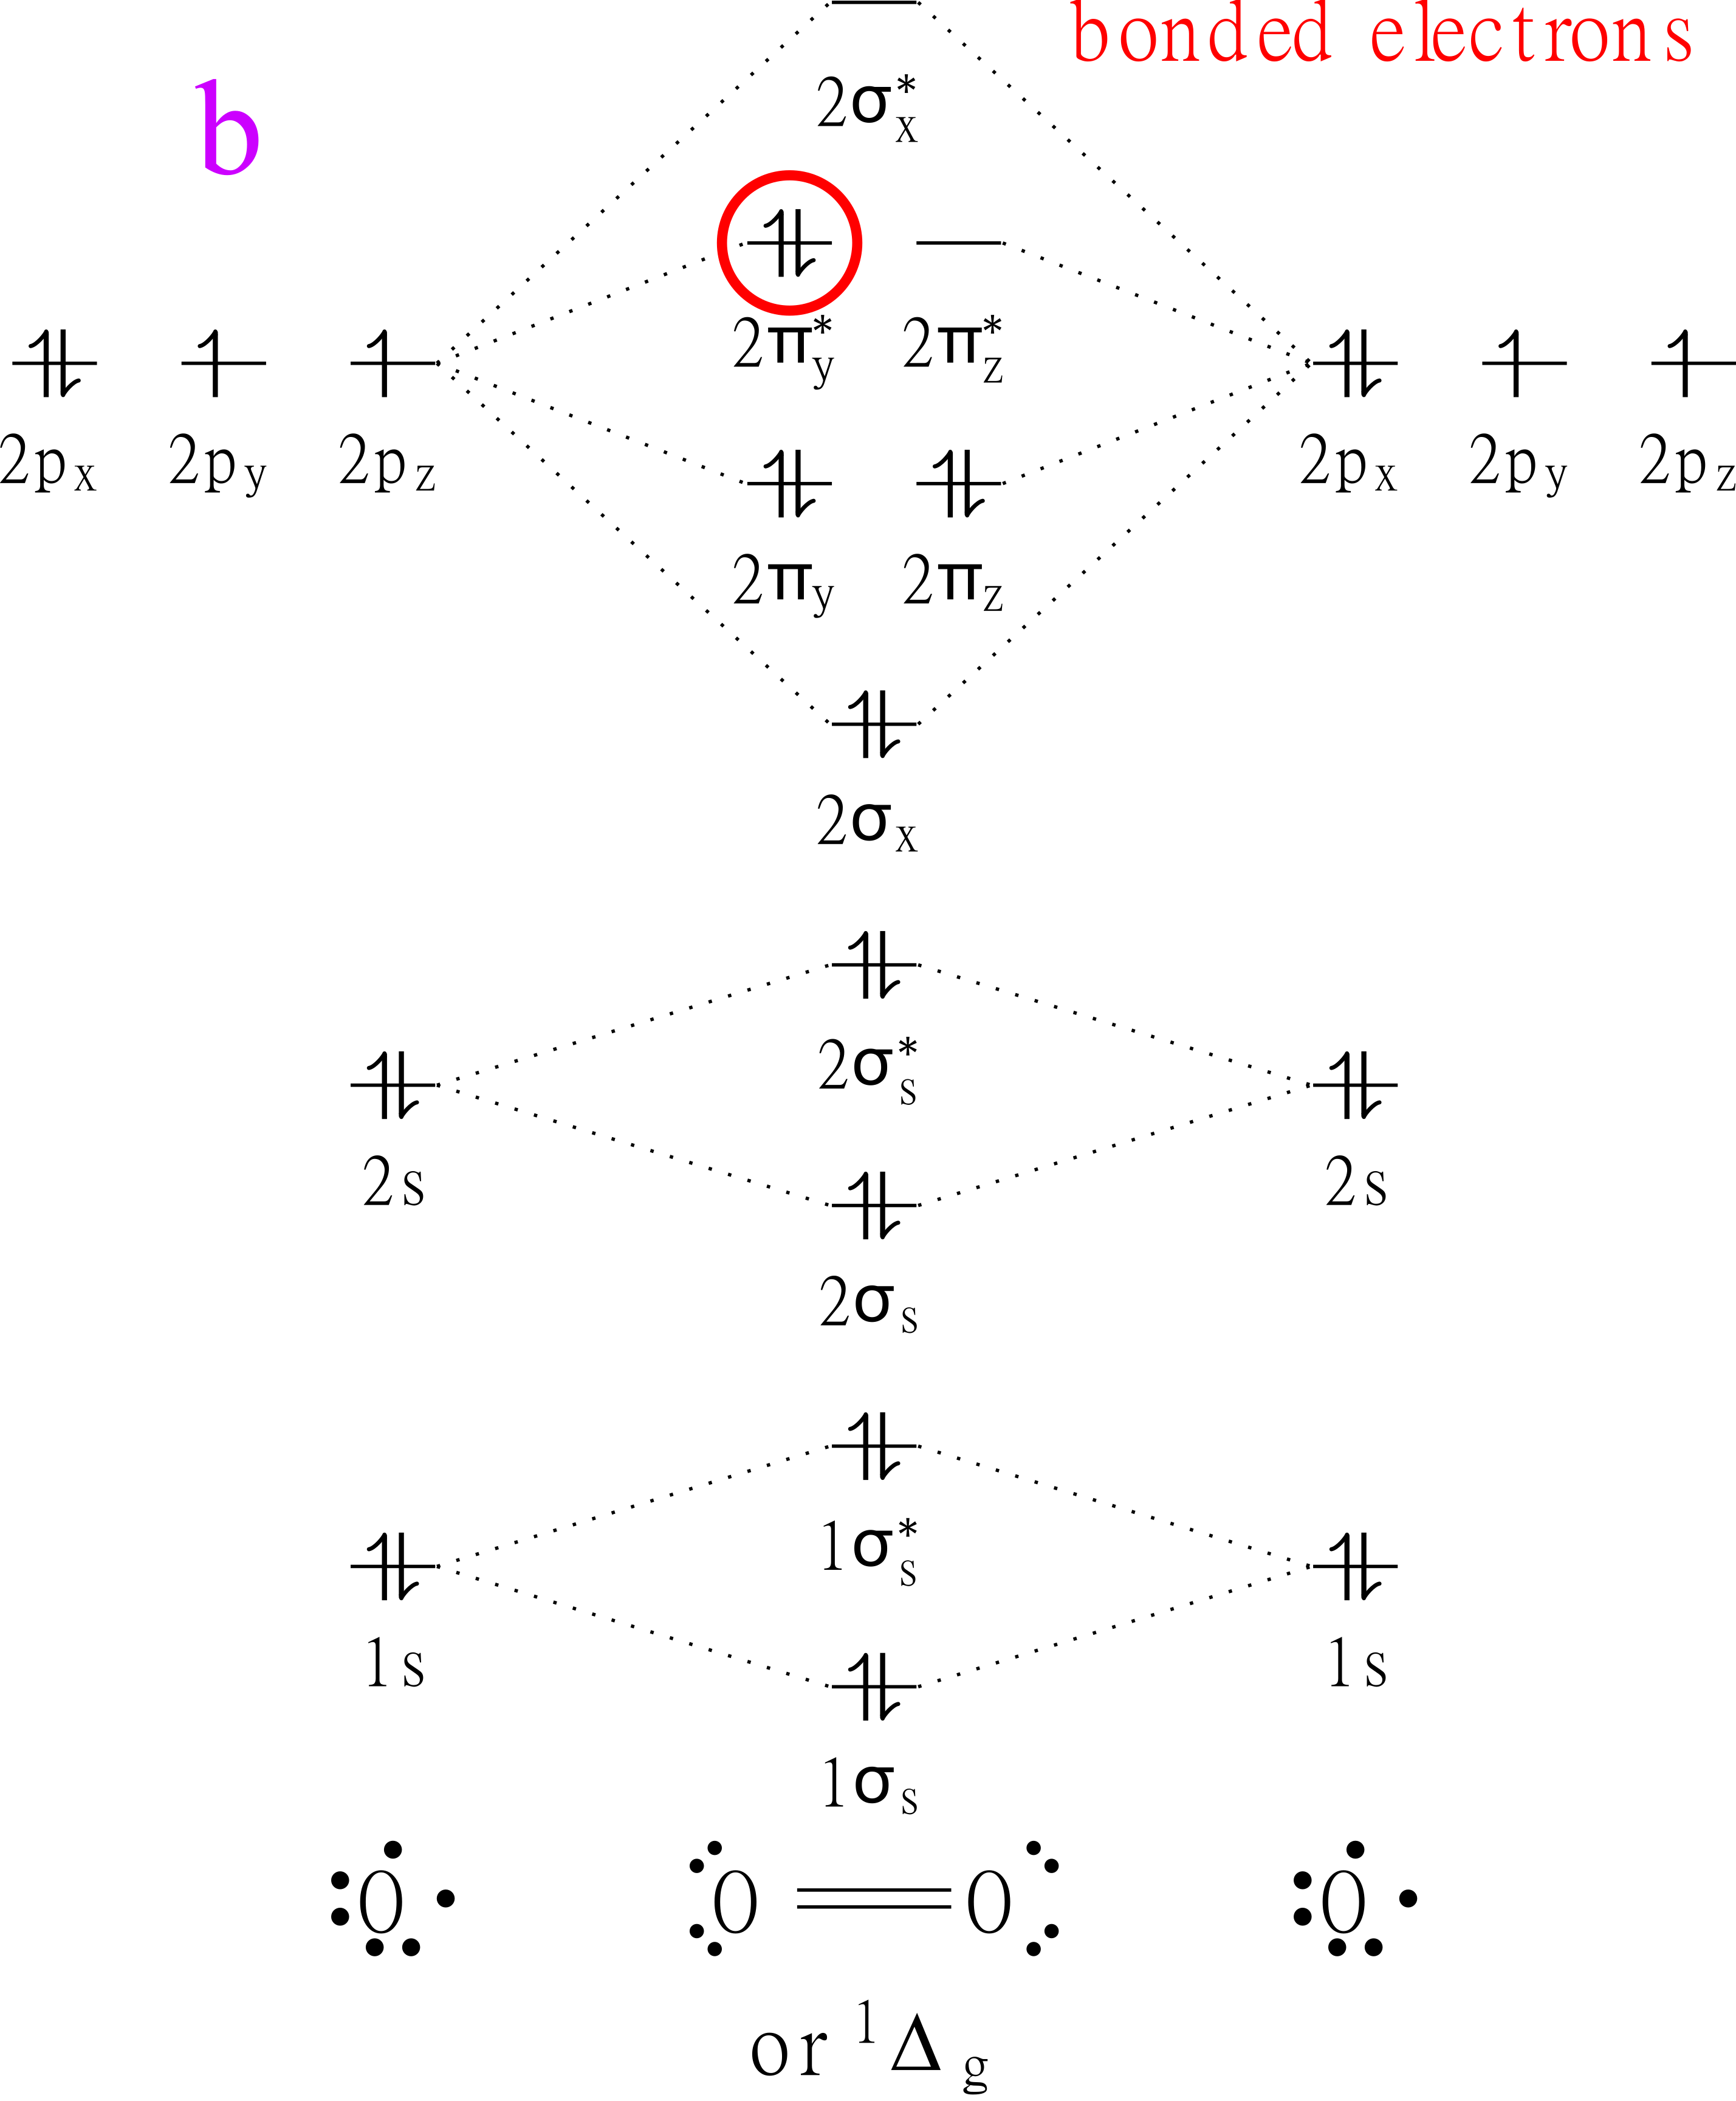
\includegraphics[width = 0.48\textwidth]{images/PDIpy/background/singlet_mo_diagram.png}
    \end{tabular}
    \caption{
        Qualitative orbital diagrams for a) $^3\Sigma_g^-$ and b) $^1\Delta_g$ configurations of diatomic oxygen. Each barbed arrow represents a single electron, and each platform represents the electronic sub-orbital of the respective label, where orbital energy increases vertically in the diagram. The distinction between a) and b) is highlighted by the red circled electrons and labels, where $^1\Delta_g$ possesses an anti-bonding $\pi^*$-bond in its HOMO that destabilizes it relative to $^3\Sigma_g^-$.
    }
    \label{mo_diagrams}
\end{figure}

\begin{figure}[t]
    \centering
    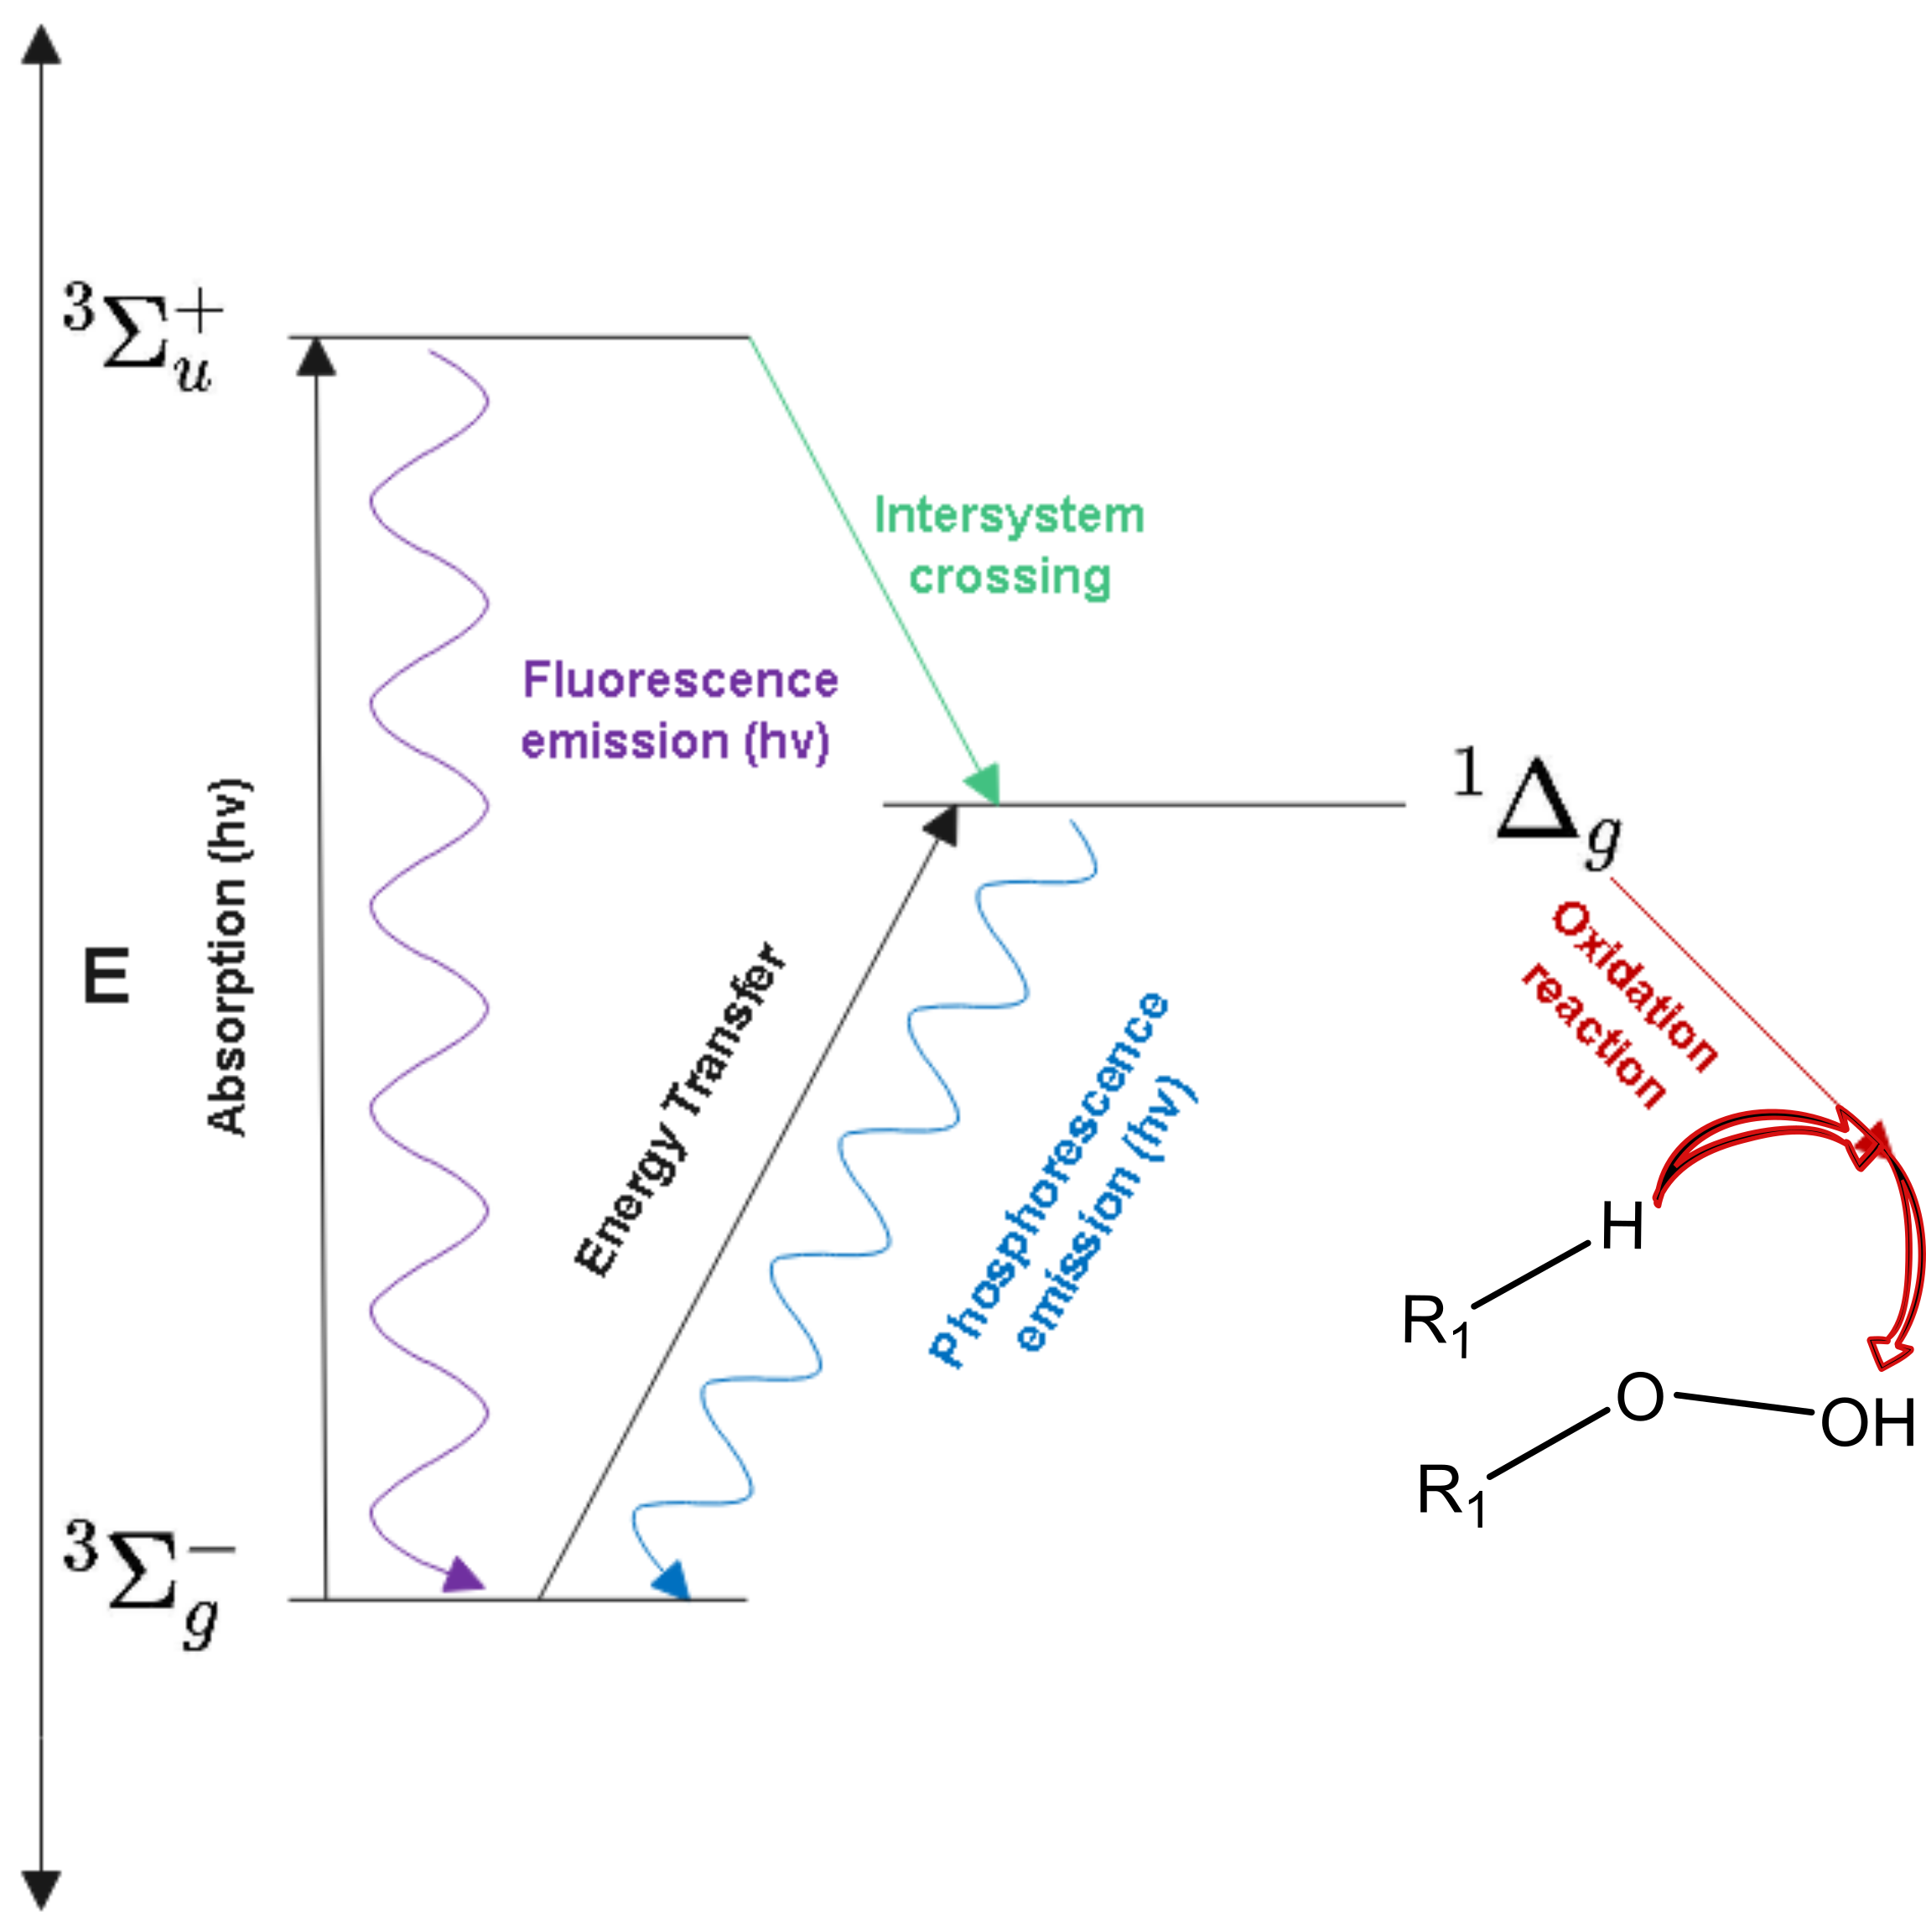
\includegraphics[width = \textwidth]{images/PDIpy/background/jablonski_diagram.png}
    \caption{
        A qualitative Jablonski energy diagram of Steps b-c of PDI. The initial excitation in PDI occurs via an energy transfer $\ce{^3\Sigma_g^- ->[energy transfer] ^1\Delta_g}$. The ROS then, while abstaining from phosphoresce, oxidizes a biological substrate to form a peroxide that gradually compounds to cause lysis.
    }
    \label{jablonski_diagram}
\end{figure}

\begin{figure}[t]
    \centering
    \includegraphics[width = \textwidth]{images/PDIpy/background/BCFA_schenck_oxidation_2.png}
    \caption{
         The reaction mechanisms of Type II oxidation and subsequent decompositions. \textbf{Step (1)} depicts the concerted \cite{Foote1968PhotosensitizedOxygen} Schenck reaction. \textbf{Step (2)} depicts the homolytic cleavage of the hydroperoxide bond to form $\ce{OH^.}$ and an oxy radical that may enter autoxidation (Type I oxidation) mechanisms. \textbf{Step (3)} depicts radical propagation via hydrogen abstraction to form another radical substrate and an alcohol byproduct. \textbf{Step (4)} is a concerted Russell reaction \cite{Russell1957Deuterium-isotopeRadicals,Howard1968TheMechanism} between two peroxides that forms a $\ce{H2O2}$, an $\alpha,\beta$-ketone, and an alcohol. The reactions of Steps (2-4) sample the wide range of possible decompositions that follow oxidation mechanisms.
    }
    \label{schenck_mechanism}
\end{figure}

\subsection{Excitation proportion} \label{excitation_proportion_estimate}

The steps for estimating the absorbed proportion of incident photons by photosensitizers, where absorbance or transmittance measurements are not available, are detailed through the following steps. a) The reported intensity of incident light from the respective light source -- i.e. irradiance ($\frac{mW}{cm^2}$), lux ($\frac{lumen}{m^2}$), or lumens (lumens) -- is converted into a quantity of incident watts $watts_{in}$ ($\frac{J}{s}$). b) This incident wattage is attenuated by the proportion of the emission spectra $spec_{em}$ that resides within the $spec_{ex}$ of the PS, 
\begin{equation}
    watt_{ex} = \frac{spec_{ex}}{spec_{em}}*watts_{in}.
\end{equation}
c) The $watt_{ex}$ is then used to calculate the moles of incident photons that strike photosensitizers per timestep 
\begin{multline} \label{photons_per_second}
    \frac{photons_{strike~PS}}{timestep}=\frac{<h\nu_{ex}>}{h*c}*watts_{ex} *\frac{s}{\Delta t}*reflection*scattering*\frac{1~mole}{N_A}*\frac{vol_{PS}}{vol_{total}},
\end{multline}
where $reflection \approx 96 \%$ and represents the proportion of incident photons that penetrate an aqueous solution \cite{Gross1993SingletLiposomes}; and $scattering \left(\frac{I_z}{I_0} = e^{-k*z}\right)$ represents the proportion of light $\frac{I_z}{I_0}$ that reaches a specified depth $z$ \cite{RobertW.1973TheSea}, where $k$ is the attenuation coefficient that is $\approx 0.04~(\frac{1}{m})$ \cite{Lorenzen1972ExtinctionPhytoplankton} for clear water. The quotient $\frac{vol_{PS}}{vol_{total}}$ describes the fraction of the solution volume where the PS resides ($vol_{total}$) that is comprised of the PS per se ($vol_{PS}$), which is calculated as the product of the quantity of PS molecules and the volume per molecule according to its molecular structure. The average excitation wavelength of the PS ($<h\nu_{excitation}>$) is calculated as the weighted average of the Soret and Q excitation bands, in proportion to their relative contribution in generating $^1\Delta_g$ \cite{Nitzan2001PhotoinactivationWavelengths,Hoenes2020PhotoinactivationWavelength}, which assumes that both excitation wavelengths are excited during the simulation. The resultant $\frac{photons_{strike~PS}}{timestep}$ from \cref{photons_per_second} is then divided by the quantity of photons that enter the system per timestep $\frac{photons_{total}}{timestep}$ to determine which fraction of photons strike a photosensitizer. 

\subsection{Deduction of inactivation via the Hill equation}

Inactivation may alternatively be deduced from oxidation through parameter manuipulation of a fitted sigmoidal curve, similar to other models \cite{Xiong1999AInactivation}. The Hill-equation \cite{Gesztelyi2012ThePharmacology} is a sigmoidal model that derives from mass-action kinetics, similar to the Michaelis-Menten kinetic model, and thus it was selected the signmoidal model for this alternative framework. A Python program for fitting the Hill-equation was developed -- the HillFit module -- with a variation of the Hill-equation \cite{Inoue2016OscillationActivation} 
\begin{equation} \label{hill_eq}
    y=bottom+\frac{(top-bottom)*x^n}{EC50^n+x^n},
\end{equation}
that introduces an additional $bottom$ parameter for more advantageous fitting. The predicted oxidation data was fitted to a hill-equation via HillFit and the parameters were subsequently adjusted in Table \ref{hill_parameters} to optimally meet the training data. The $top$ parameter of \cref{hill_eq} is adjusted asymptotically to a limit that follows an subtly different empirical expression for planktonic $1-10^{-\Omega}$ than biofilm $1-10^{-0.7-\Omega }$ simulations, where $\Omega = wattage^{\frac{1}{5}}-log10(1-final_{oxidation\_proportion})$. This limit manifests in the predicted inactivation being $\approx [1,2]-log$ greater than the predicted oxidation, which implicitly specifies an oxidation thereshold of $\approx [1,10]\%$. The different parameter adjustments between sessile and planktonic systems may be explained that numerous chemical influences, such as diffusion rates, are not explicitly considered in our kinetic model. The regression plots for the fit of the Beirao et al. training data is depicted in Figure \ref{hill_regression}. The very precise fitting -- $R^2 > 0.996$ -- supports that the Hill-equation is an accurate description of our kinetic PDI model, and conversely that our model fundamentally describes a biochemical relationship.

\begin{figure}
    \centering
    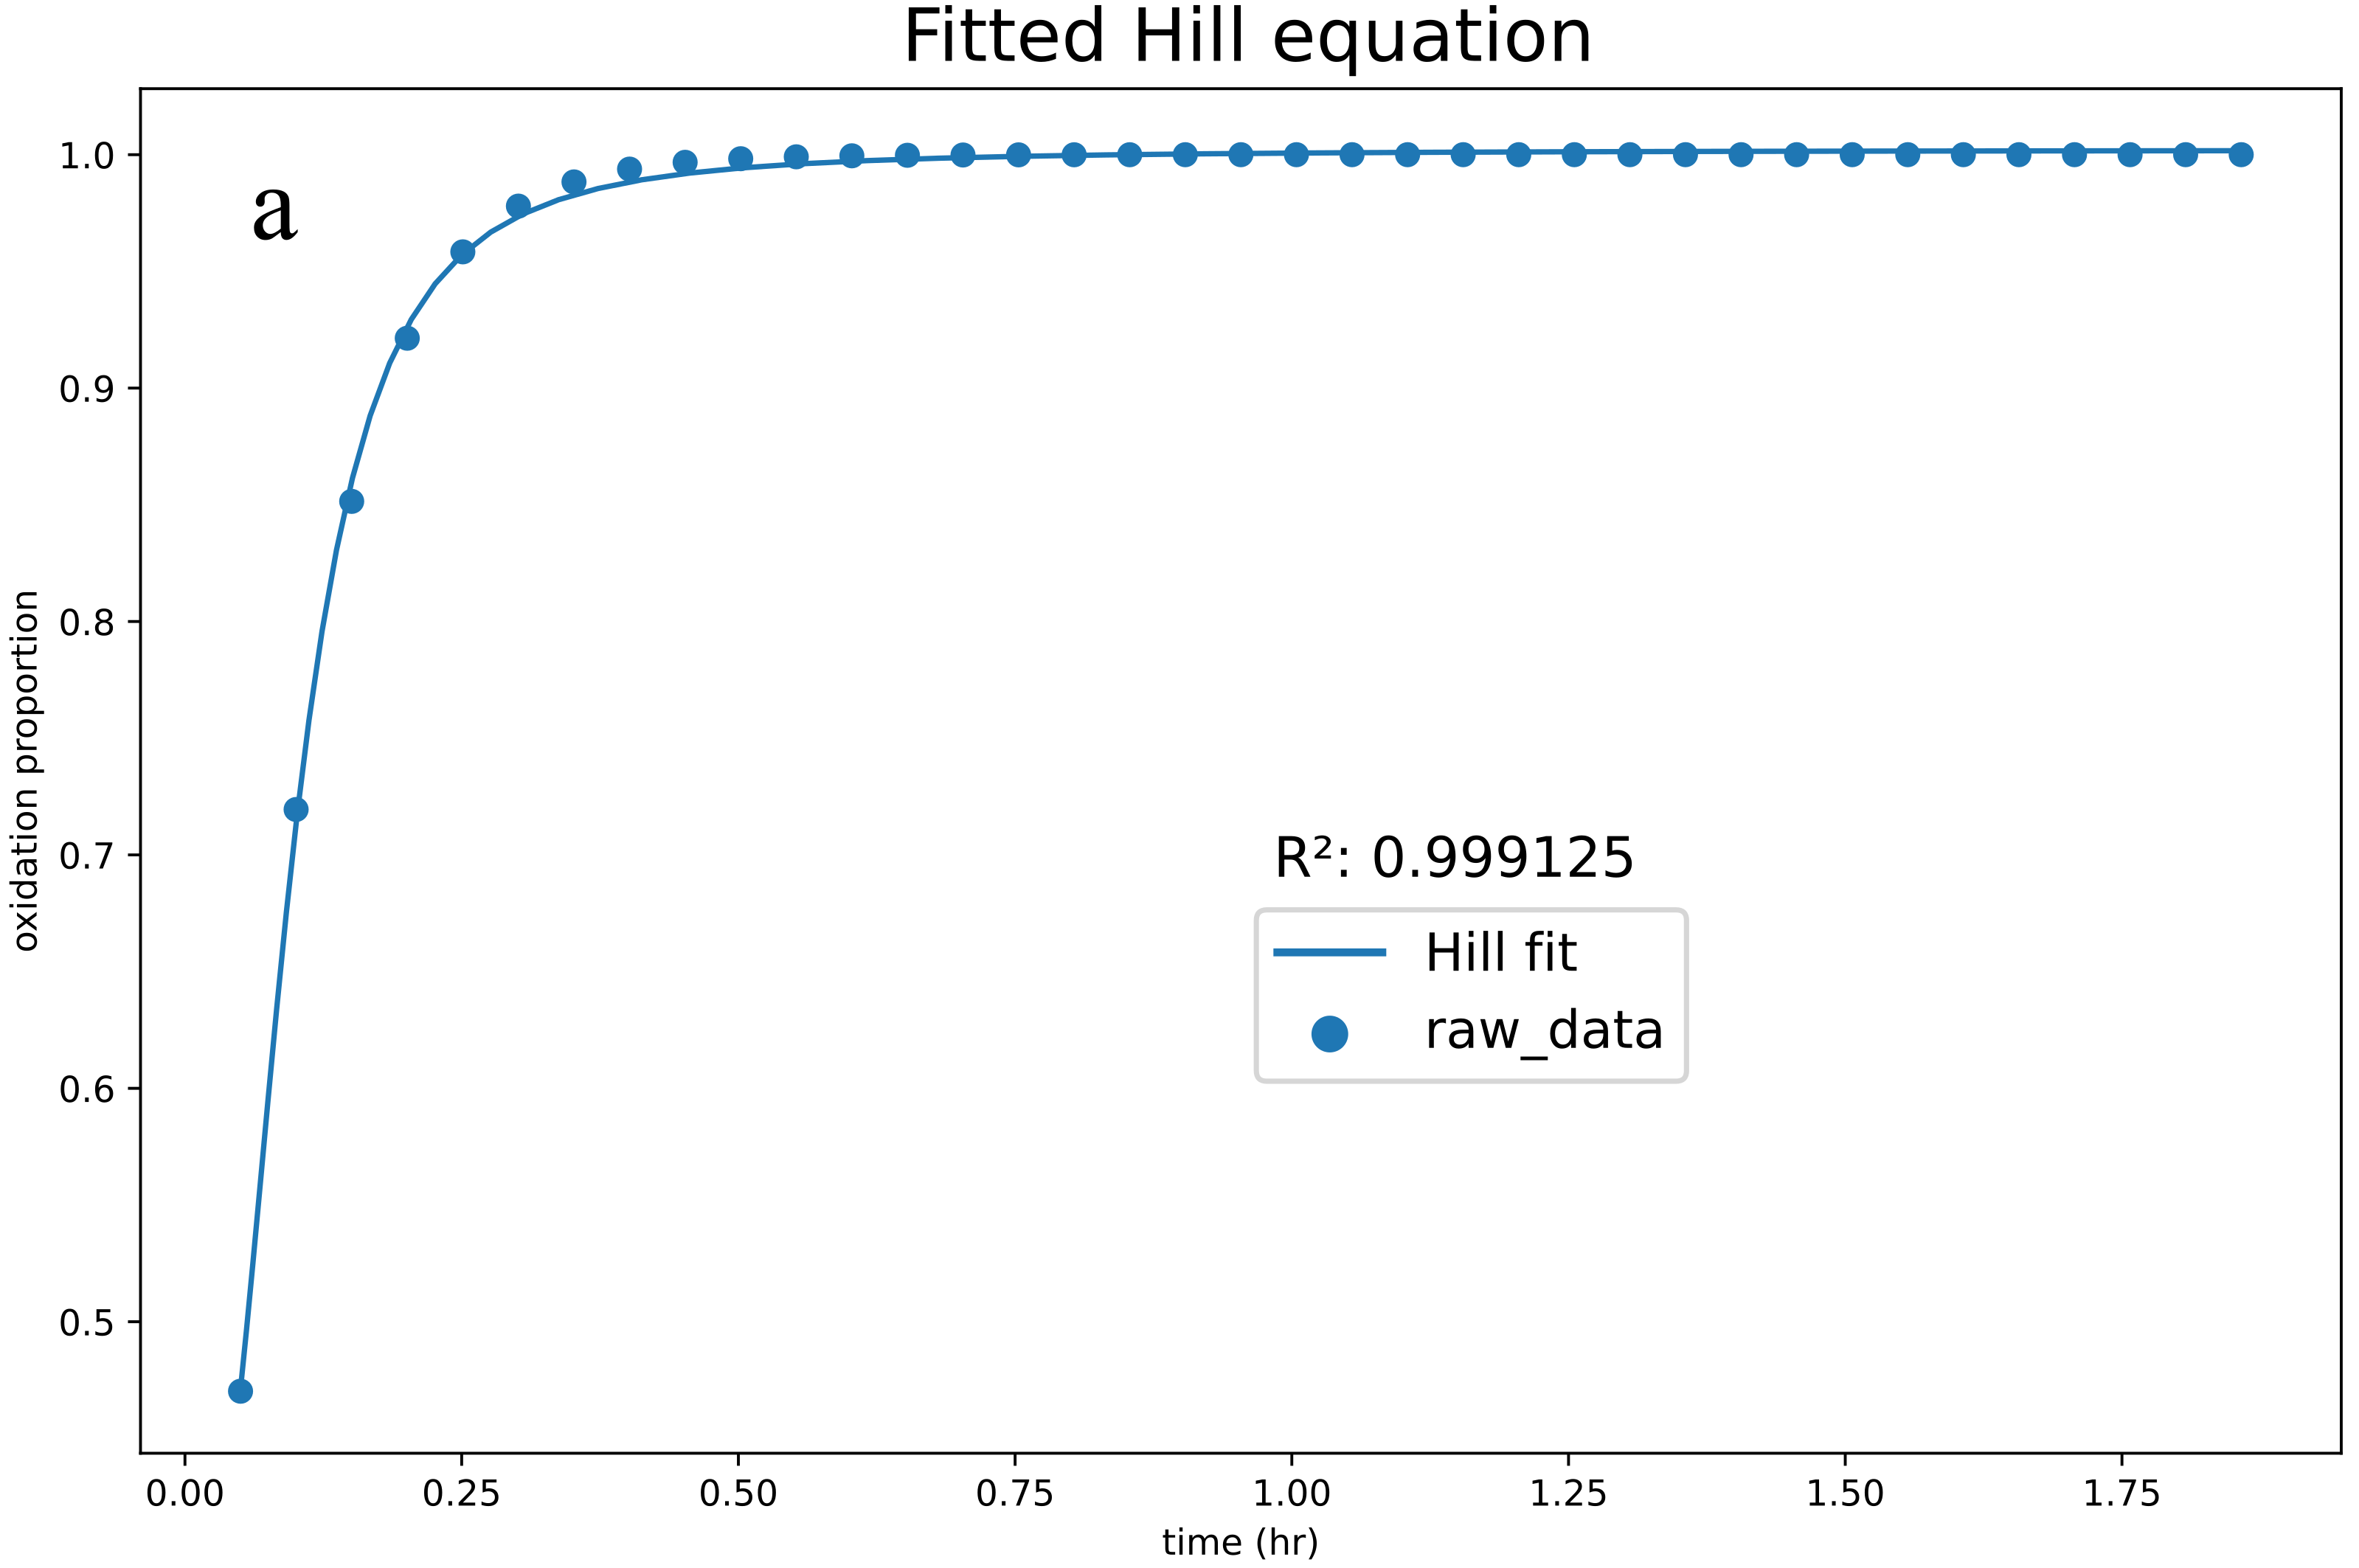
\includegraphics[width = 0.9\textwidth]{images/PDIpy/training/10uM_regression.png}
    \vspace{5mm}
    \midrule
    \vspace{5mm}
    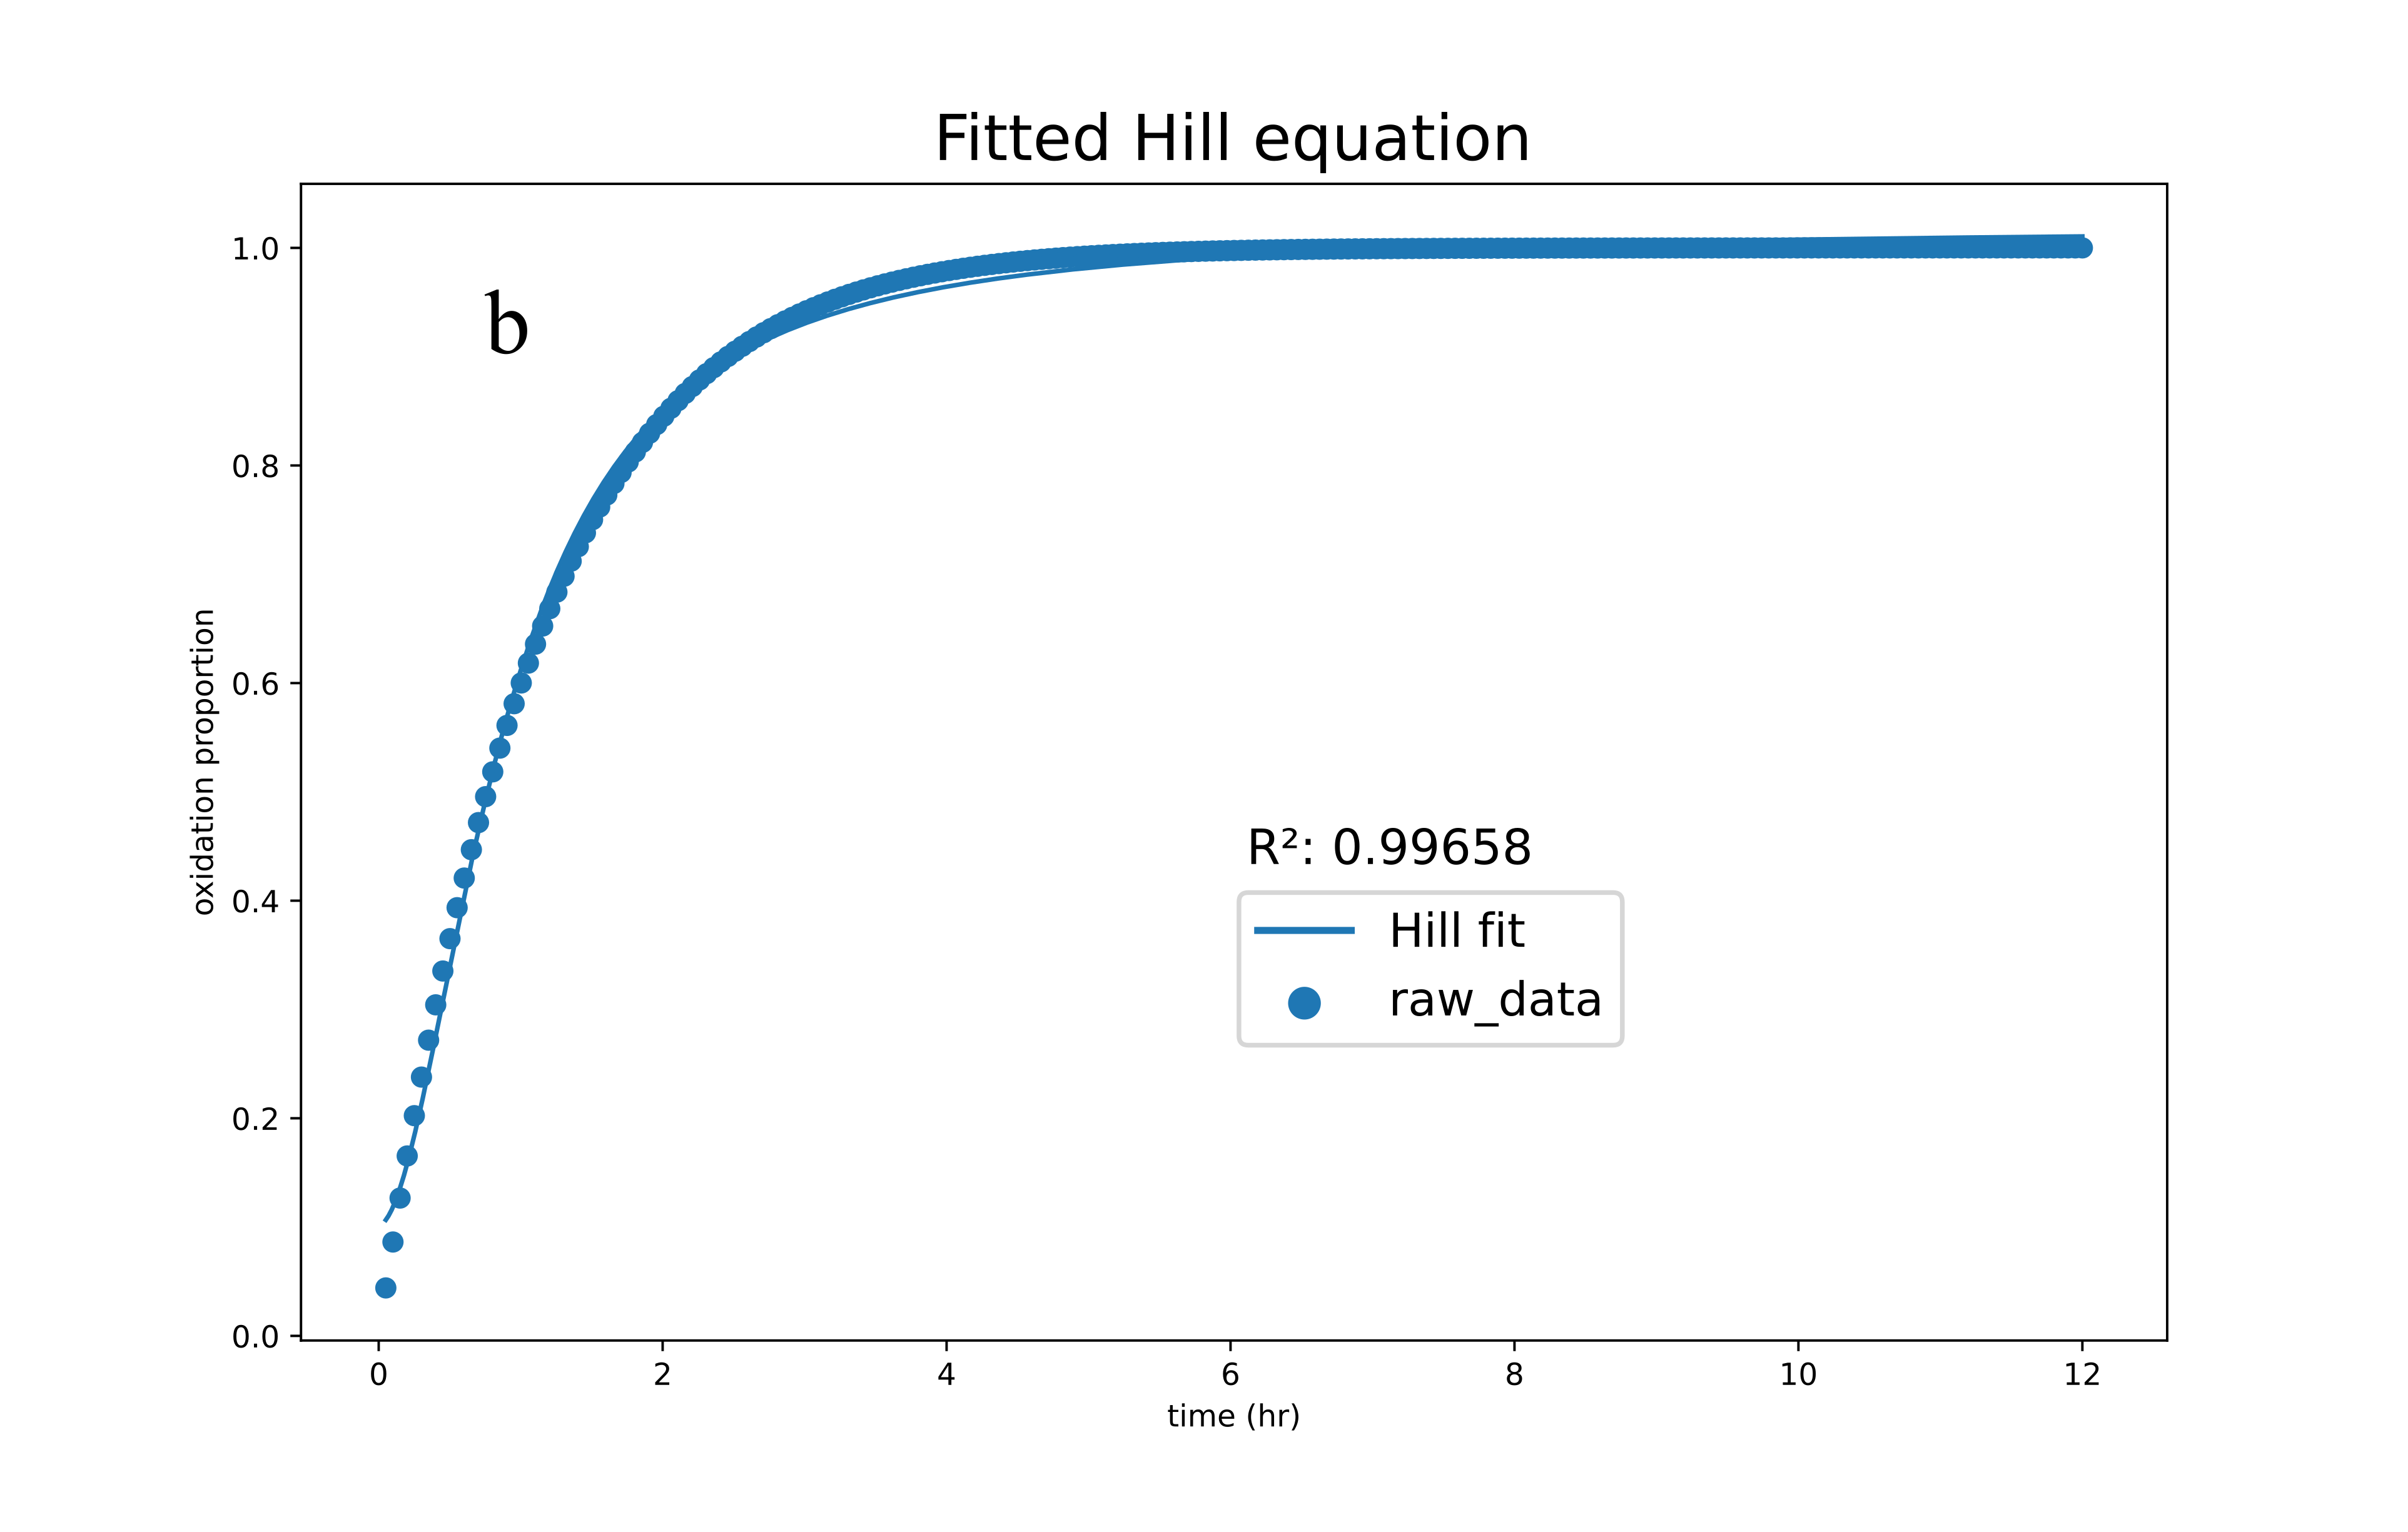
\includegraphics[width = 0.9\textwidth]{images/PDIpy/training/10uM_biofilm_regression.png}
    \caption{
        The Hill-equation regressions for the oxidation plots of the Beirao et al. training data for a) planktonic and b) sessile states. The high $R^2$ correlation supports that our chemical model of PDI recreates a sigmoidal biochemical relationship. The greater number of data points in panel b) is the consequence of a far longer simulation time than the simulation of panel a).
    }
    \label{hill_regression}
\end{figure}

% \begin{table}
%     \centering
%     \begin{tabular}{l|c|c}
%         \textbf{Bacterial state} & \textbf{Hill parameter} & \textbf{Adjustment} \\
%         \multirow{2}{}{Planktonic} & EC50 & -76\% \\
%          & nH & +100\% \\
%     \end{tabular}
%     \caption{
%         The Hill parameters adjustments that are enacted to create the inactivation plot for simulations of planktonic systems. 
%     }
%     \label{hill_parameters}
% \end{table}

\subsection{Oxidized membrane region}
The region of the bacterial membrane that is oxidized by cross-linked PSs may be a small fraction of the total membrane, provided that the bacterium does not have a tremendous angular momentum. This is not presently captured by our model, but the following logic could incorporate this concept into the model. The oxidized region of a coccus bacterial cell can be determined from the cellular radius and volume
\begin{equation}
    radius_{cell} = \sqrt[3]{3*\frac{volume_{cell}}{4\pi}}~.
\end{equation}
The membrane volume is calculated
\begin{equation}
    volume_{membrane} = \frac{4\pi}{3}*(radius_{cell}^3 - (radius_{cell}-th_{membrane})^3)
\end{equation}
there the thickness of the cytoplasmic membrane $\approx 4 nm$. The volume of oxidized membrane is then calculated
\begin{equation}
    volume_{oxidized} = volume_{membrane}*\frac{angle_{oxidized}}{360}~,    
\end{equation}
where the $angle_{oxidized}$ describes the angle in degrees from vertical at which the farthest $^1\Delta_g$ reaches the mebrane. The fraction of the membrane volume that is oxidized is then calculated 
\begin{equation}
    oxidized = \frac{volume_{oxidized}}{volume_{membrane}} 
\end{equation}
and applied to augment the effective oxidation proportion
\begin{equation}
    oxidation_{proportion,new} = \frac{oxidation_{proportion,old}}{oxidized}~.
\end{equation}

\subsection{Sensitivity analyses}

\paragraph{Light source \& emission}
The sensitivity of simulation results to the light source -- incandescent, LED, or fluorescent -- was explored. The comparison of incandescent and LED light sources, where LED and fluorescent were nearly indistinguishable, is depicted in Figure \ref{light_source}. These simulated differences are solely attributed to differences in the proportion of emitted photons that are within the visible spectrum, since PDIpy does not current resolve the intensity of specific emitted wavelengths or consider the inactivation effects of heat from incandescent bulbs. The visible proportion of the emitted wavelengths was determined in Figure \ref{light_emission} to have minimally consequence above 20\%.

\begin{figure}
    \centering
    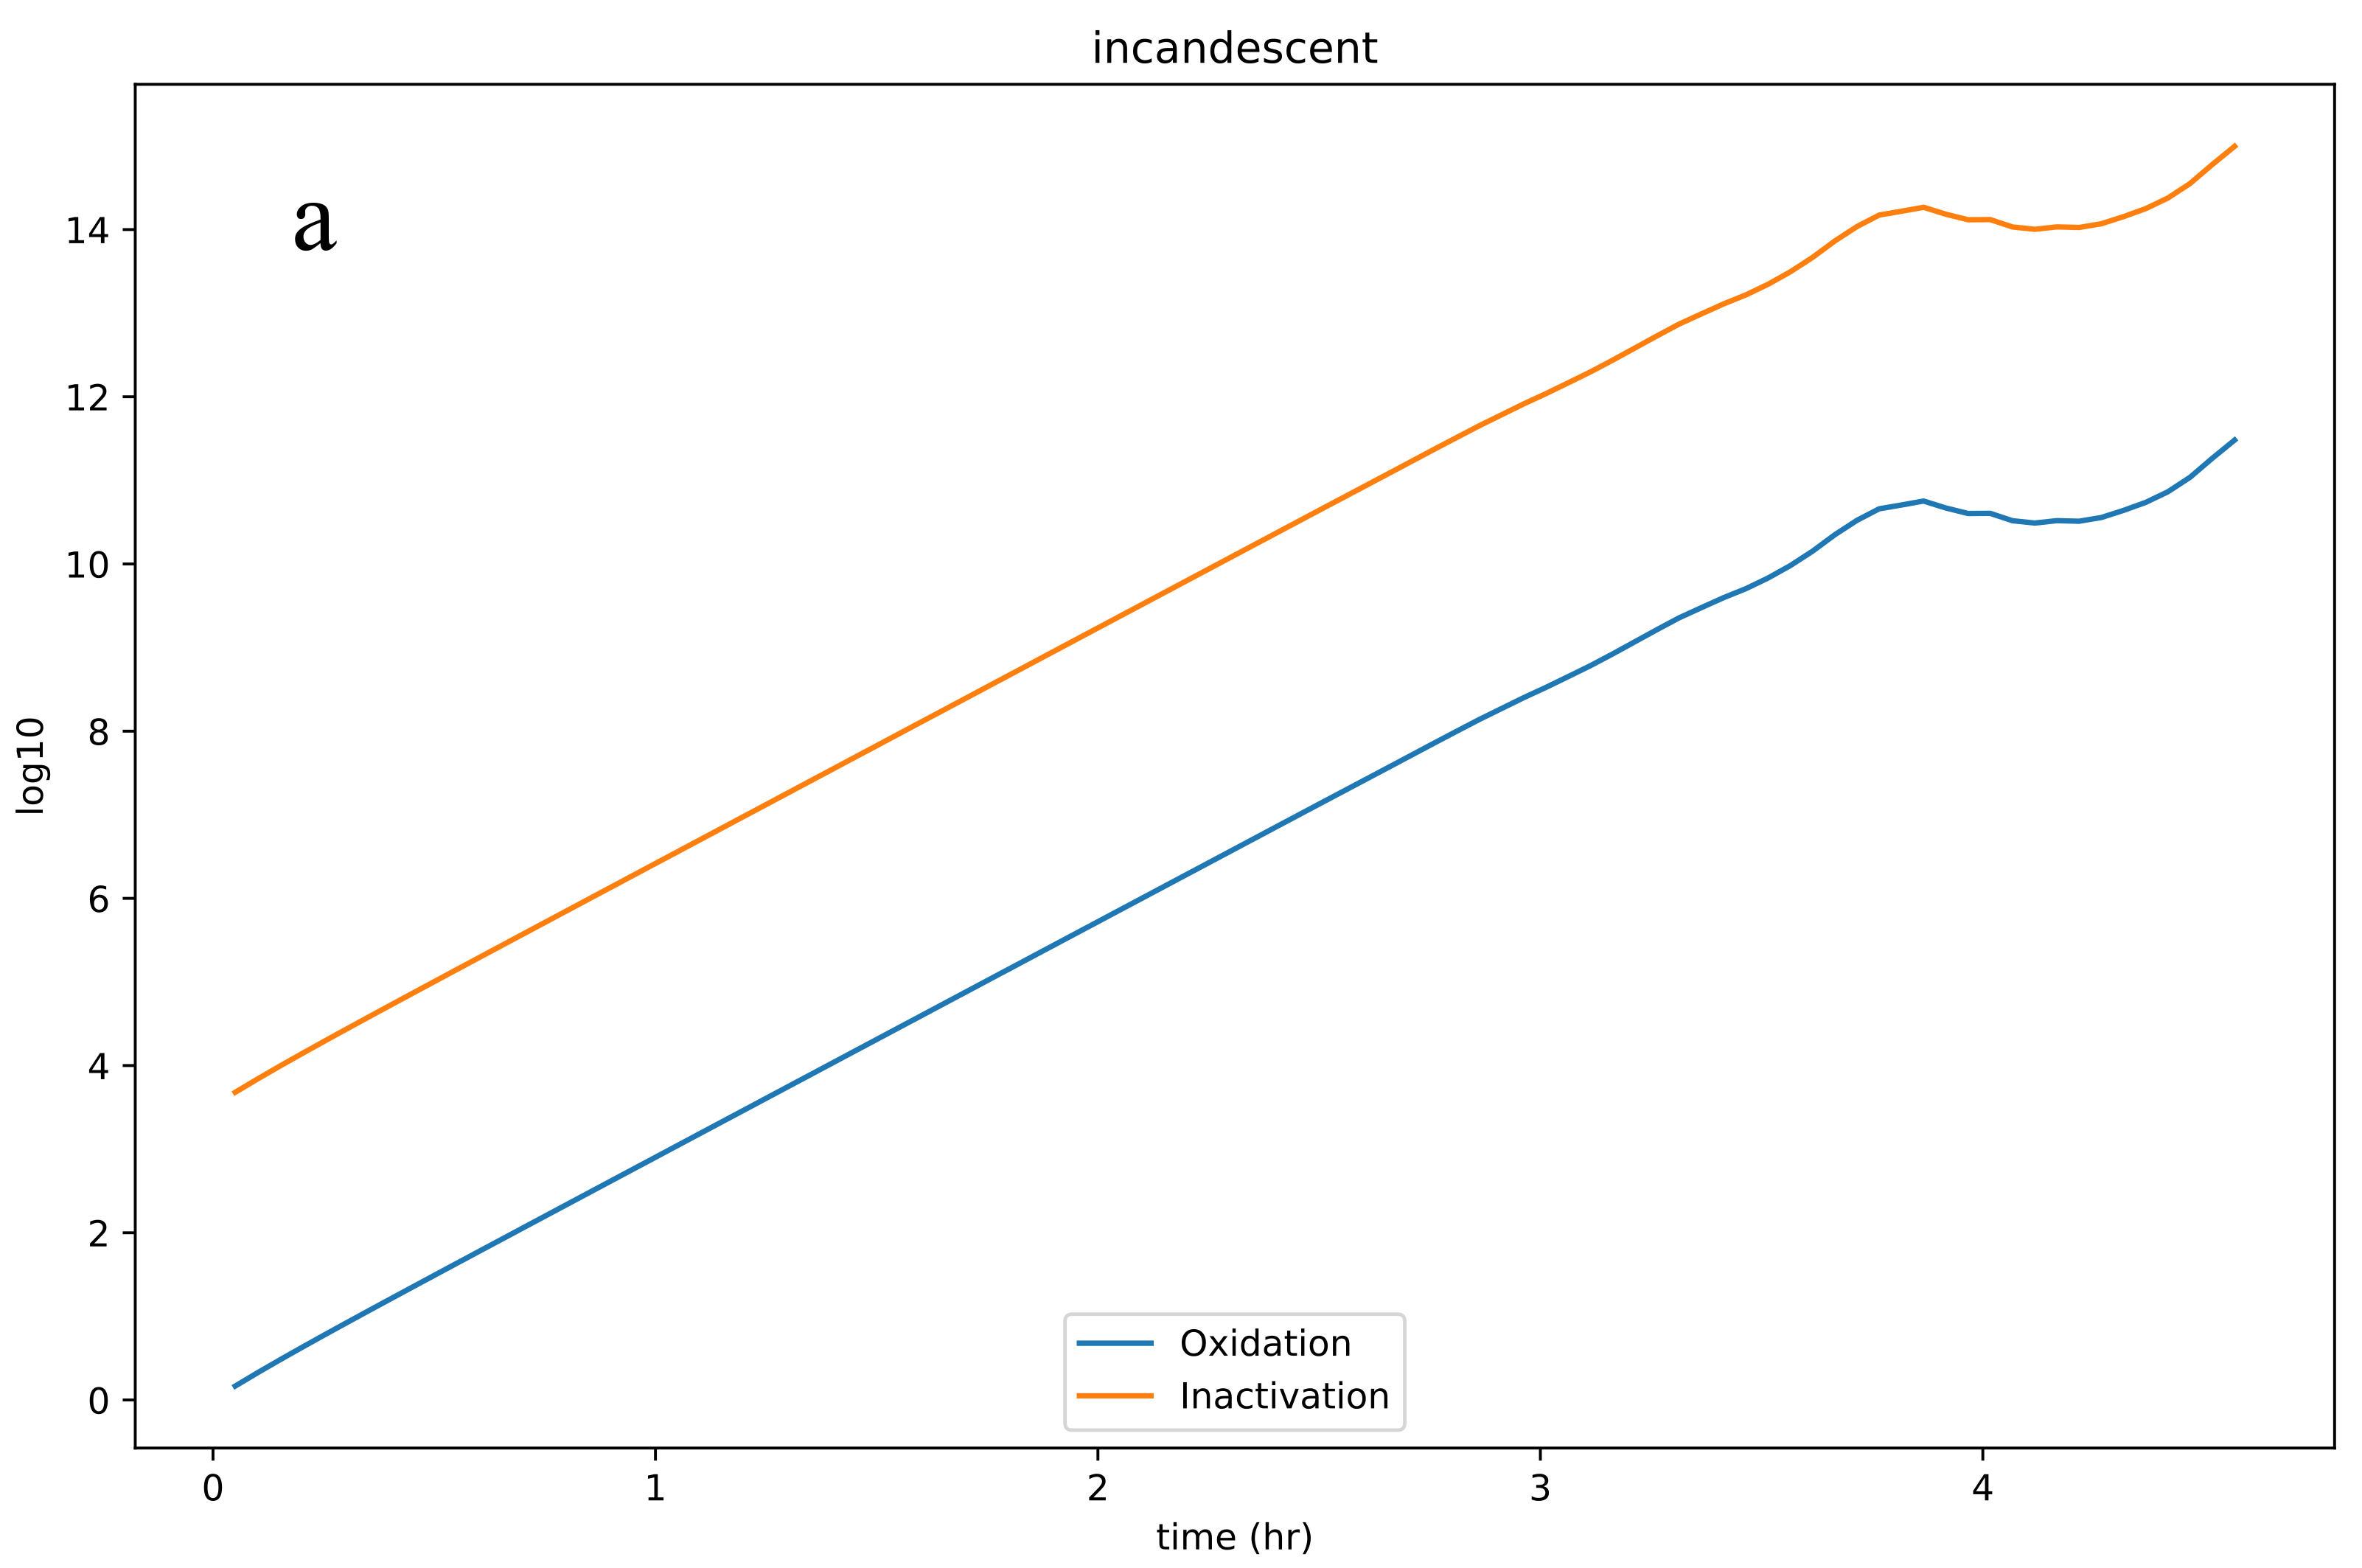
\includegraphics[width = 0.9\textwidth]{images/PDIpy/sensitivity_analyses/light_source/incandescent.png} \\
    \vspace{5mm}
    \midrule
    \vspace{5mm}
    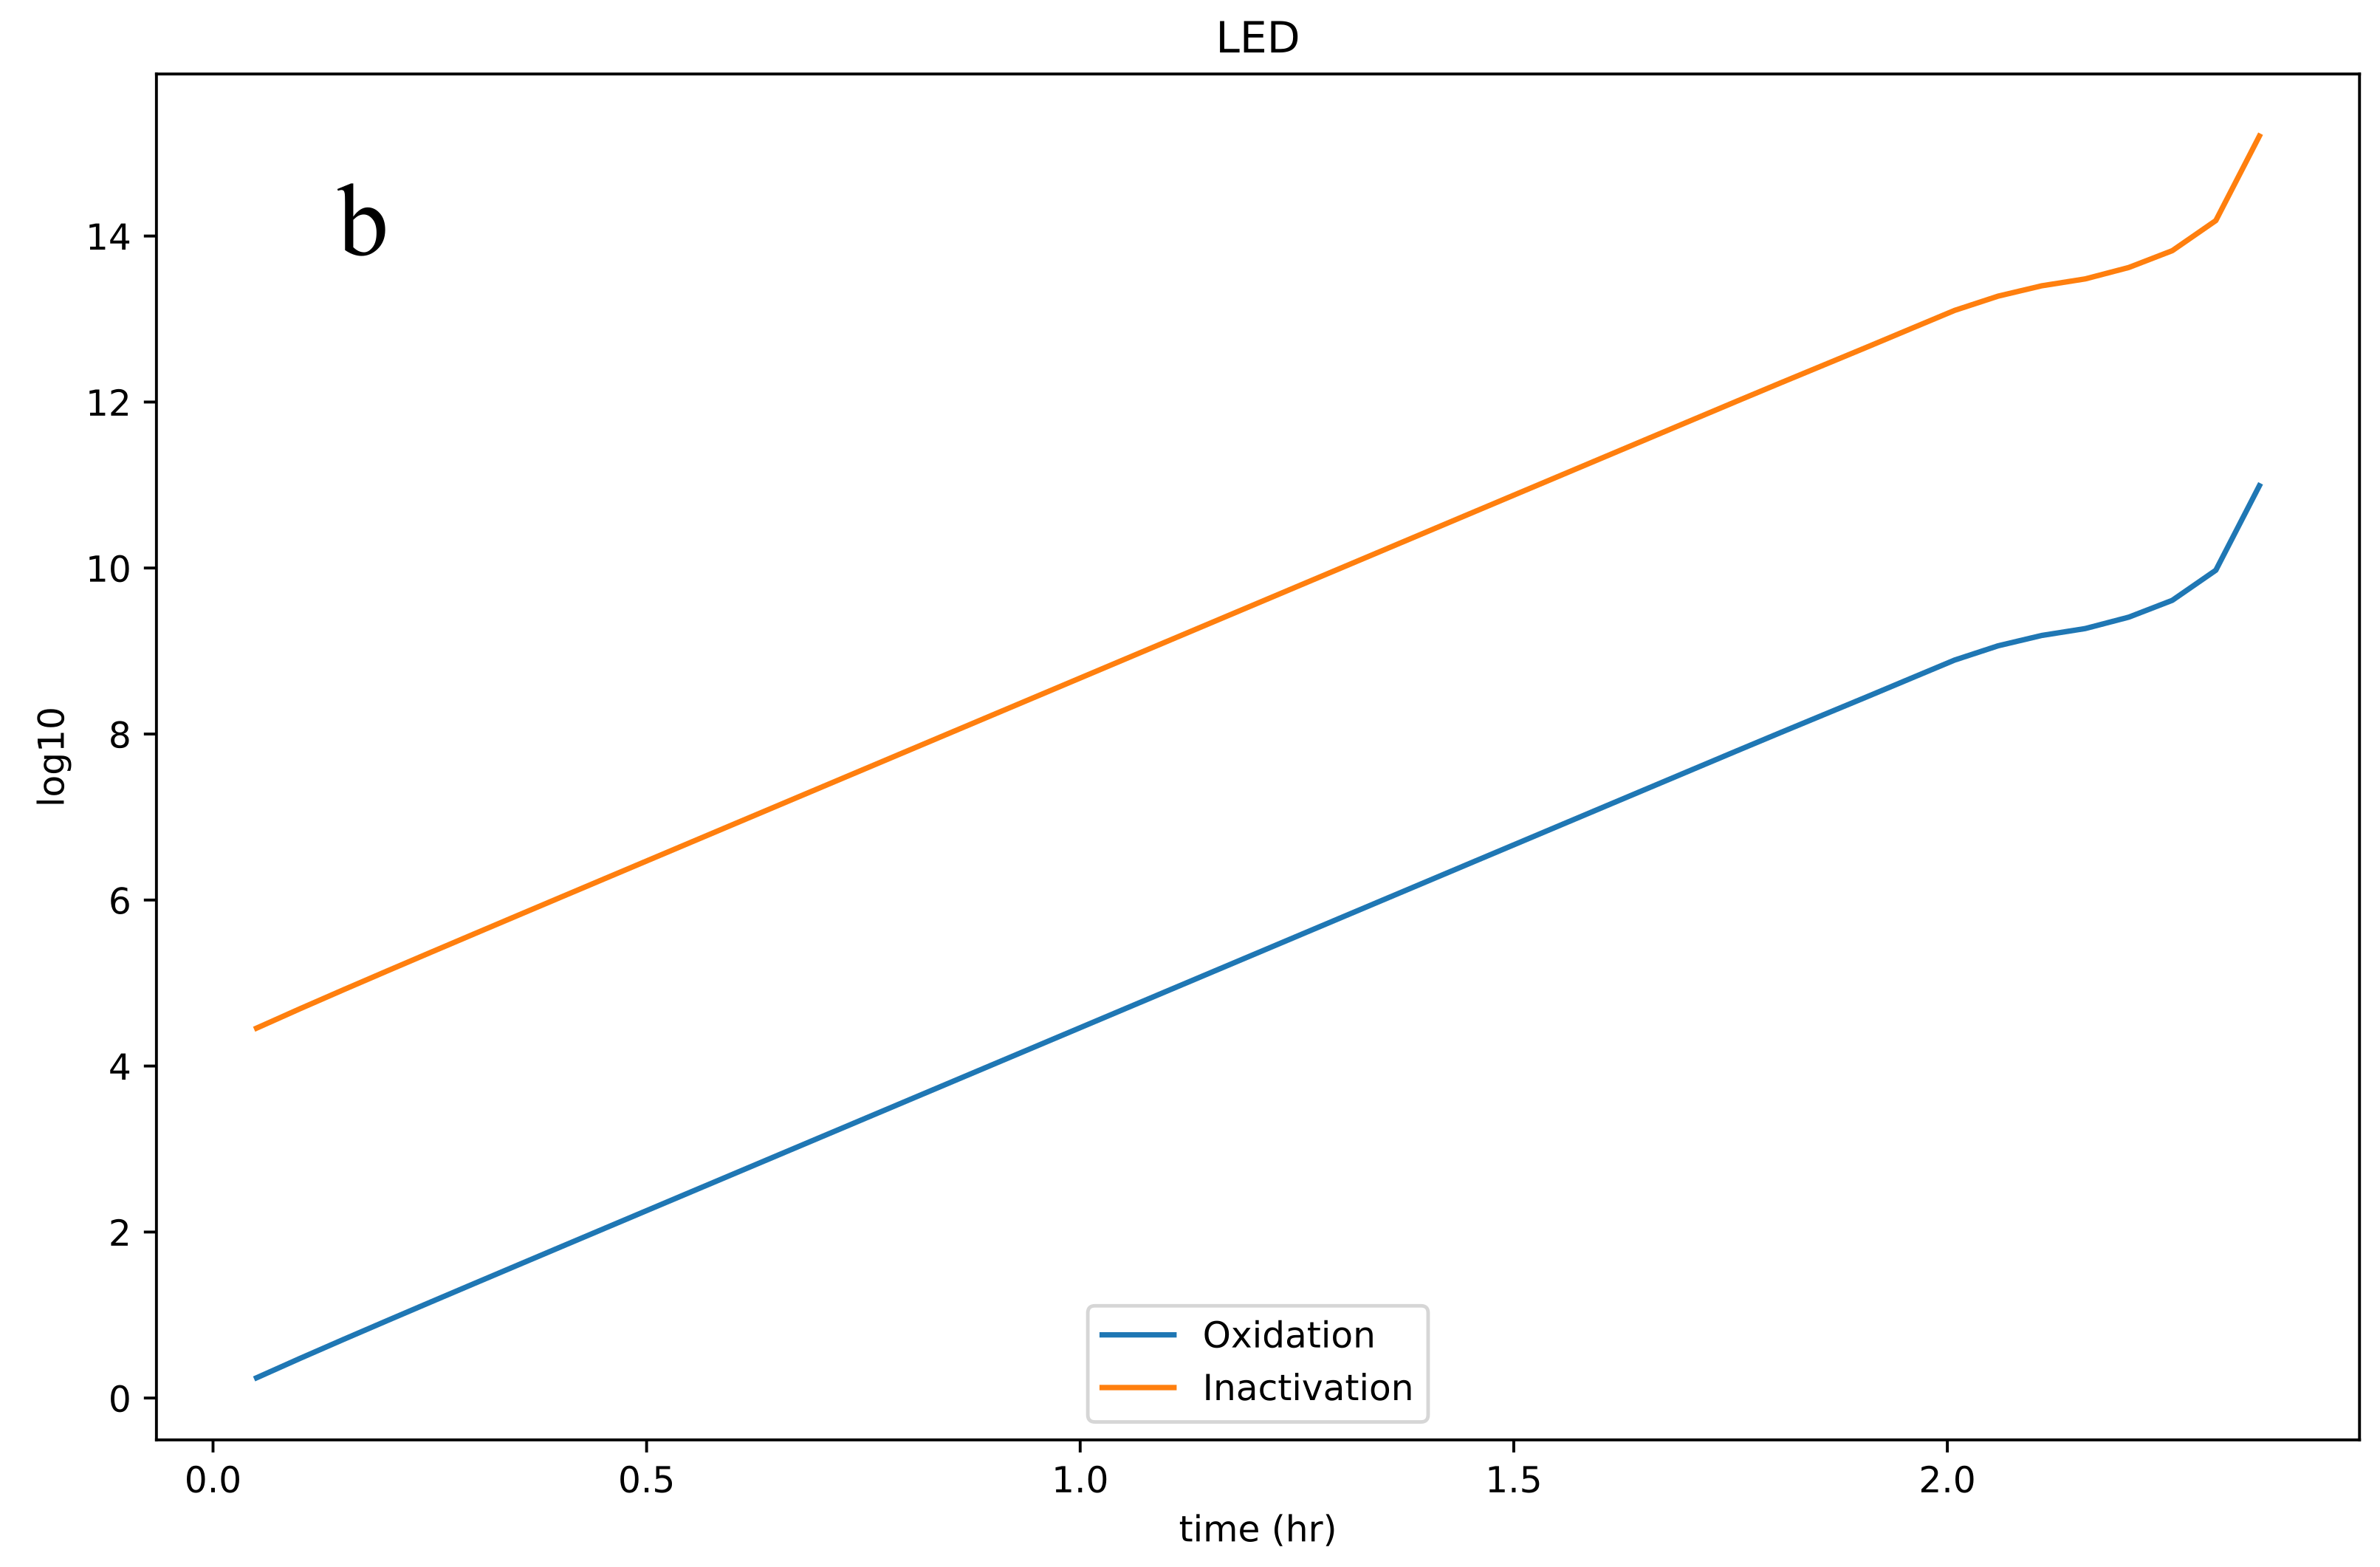
\includegraphics[width = 0.9\textwidth]{images/PDIpy/sensitivity_analyses/light_source/LED.png}
    \caption{
        A comparison of the same experiment under a) incandescent and b) LED light sources. The discrepancy between the inactivation of the two sources is attributed to the proportion of emission that resides in the visible spectrum.
    }
    \label{light_source}
\end{figure}

\begin{figure}
    \centering
    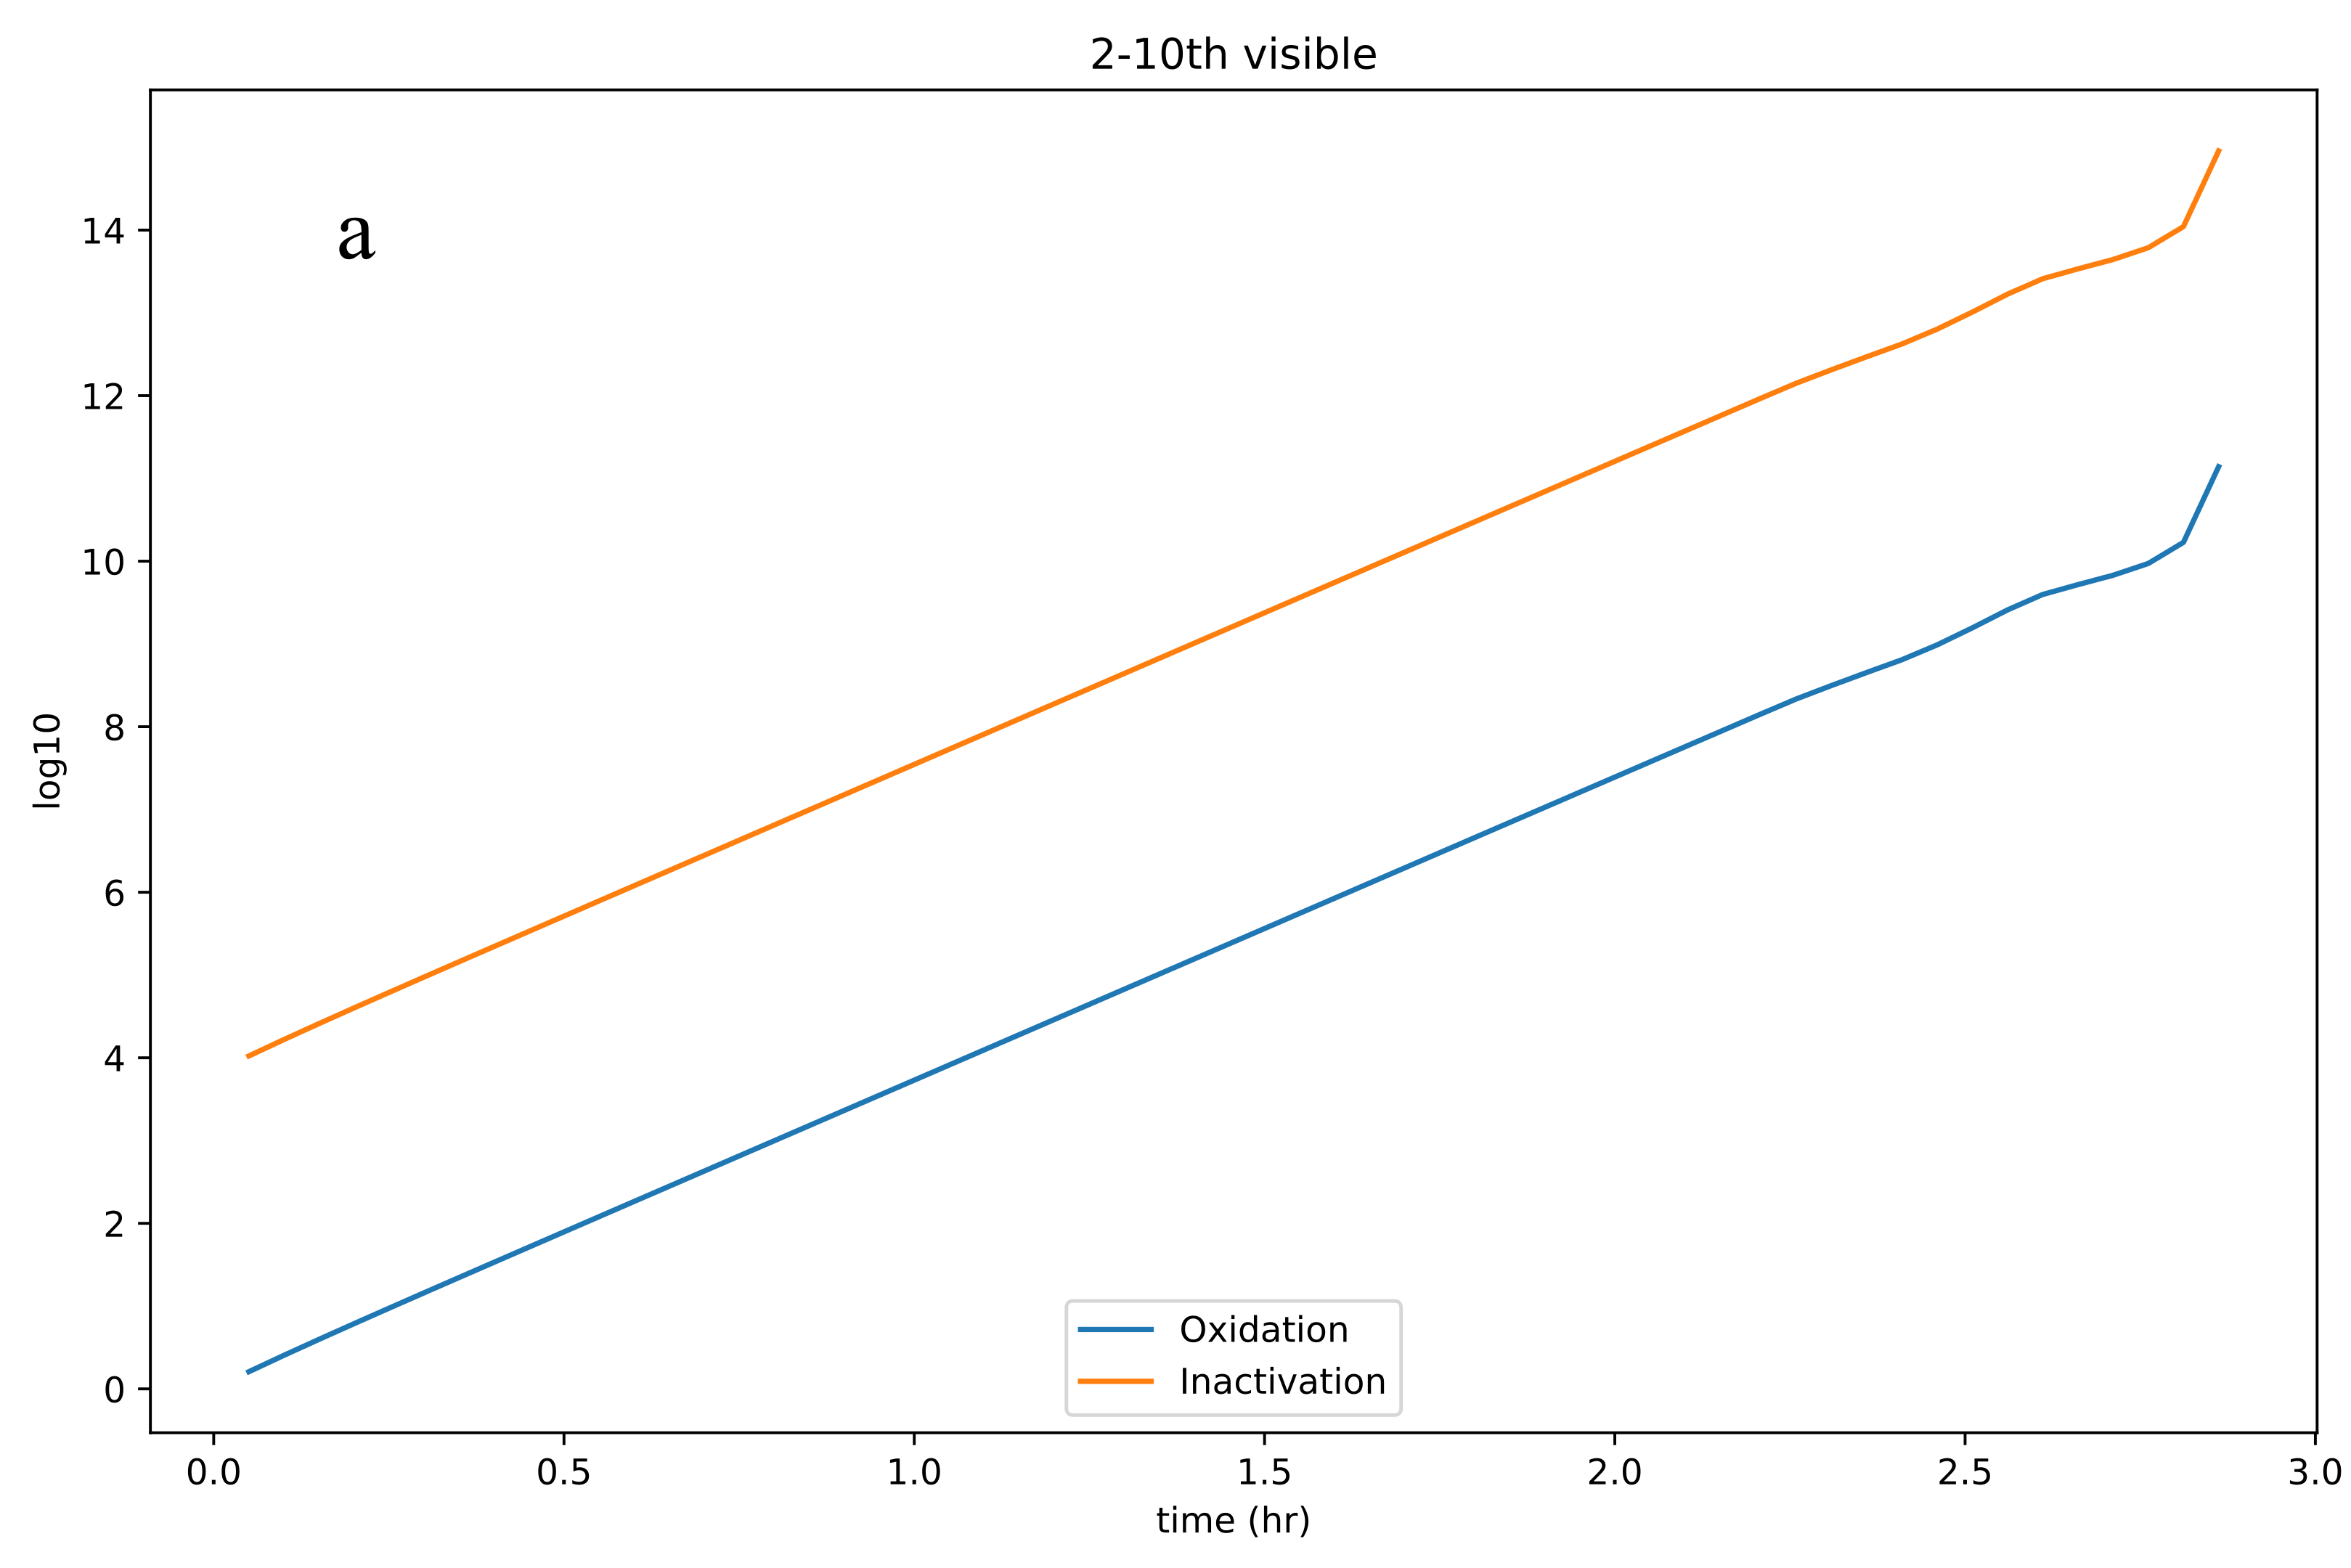
\includegraphics[width = 0.9\textwidth]{images/PDIpy/sensitivity_analyses/light_emission/20_visible.png} \\
    \vspace{5mm}
    \midrule
    \vspace{5mm}
    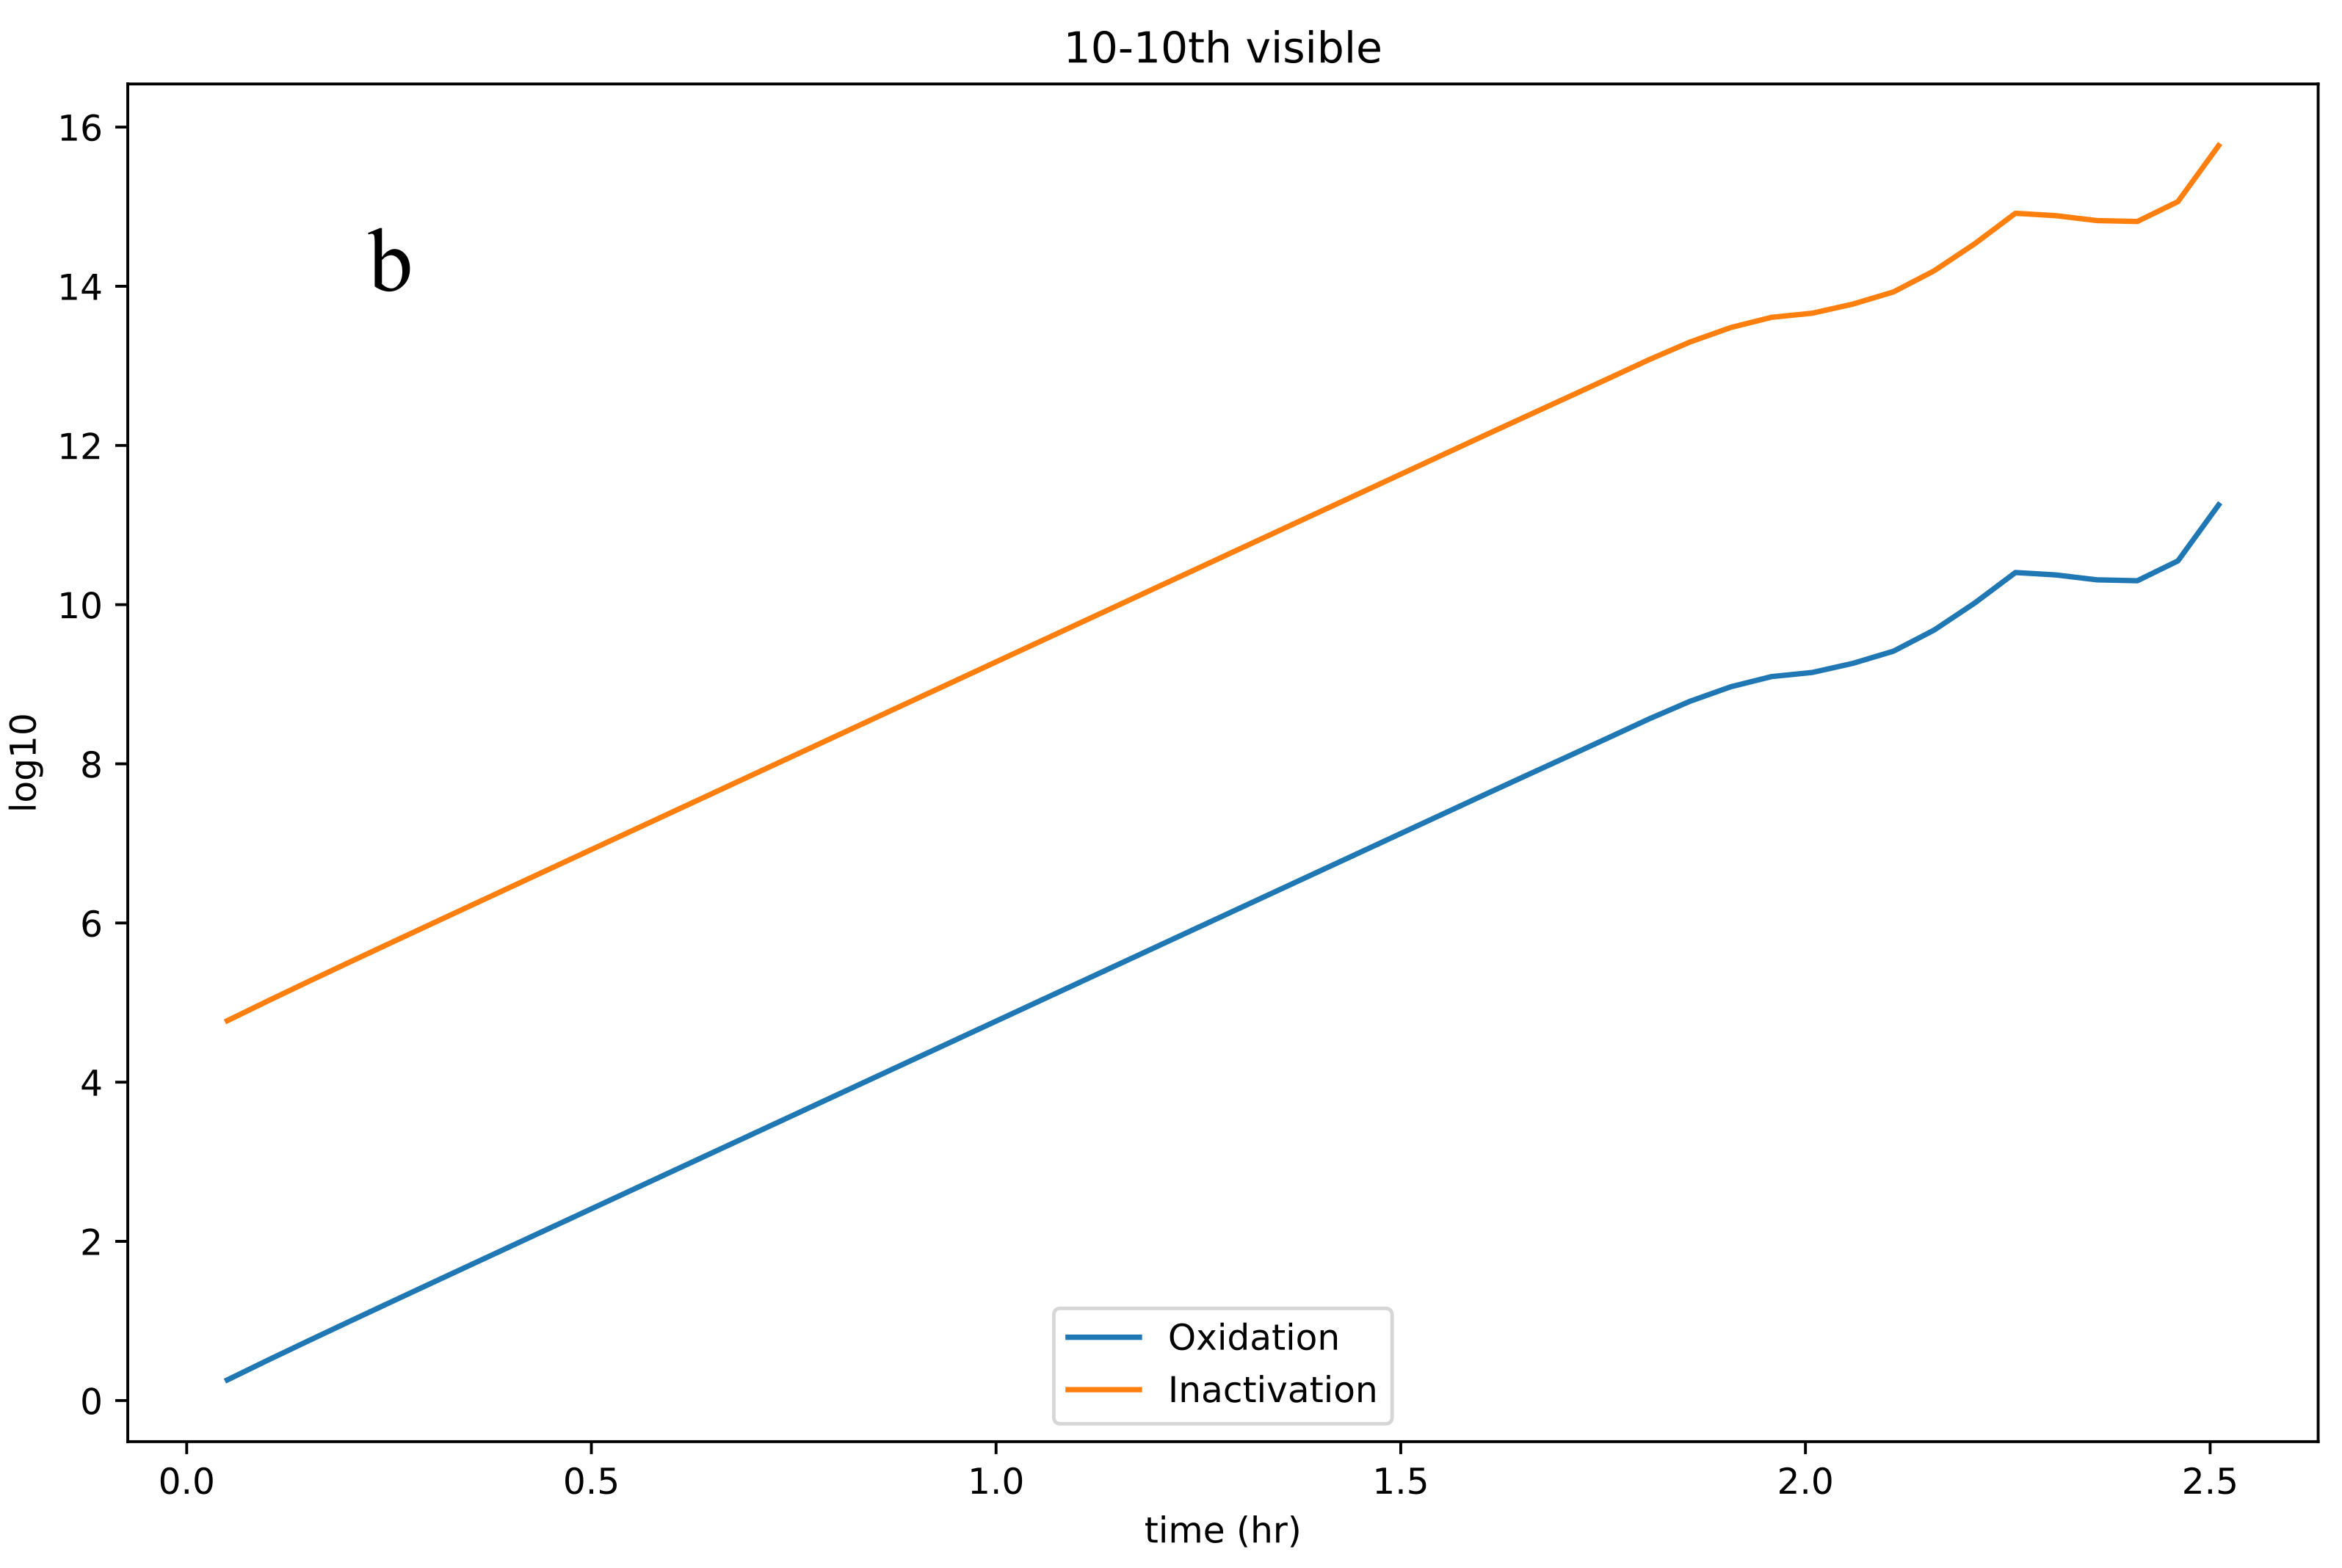
\includegraphics[width = 0.9\textwidth]{images/PDIpy/sensitivity_analyses/light_emission/100_visible.png}
    \caption{
        A comparison of the same experiment with a light source that possesses a) 20\% visible light and b) 100\% visible light, where the former value appears -- for these simulation conditions -- to be the threshold beyond which the proportion of visible light does not substantial effect inactivation rates. This threshold is likely dependent upon the quantity of incident watts; in which case, this threshold is not broadly generaliazable for all simulation conditions.
    }
    \label{light_emission}
\end{figure}

\paragraph{Bacterial CFU/mL}
The influence of bacterial $\frac{CFU}{mL}$ upon the rate of oxidation in PDIpy was tuned to yield the trend that is depicted in Figure \ref{bacterial_cfus}, where the rate of oxidation is inversely proportional with the $\frac{CFU}{mL}$. This is intuitive, where larger bacterial populations requires more time to eradicate.

\begin{figure}
    \centering
    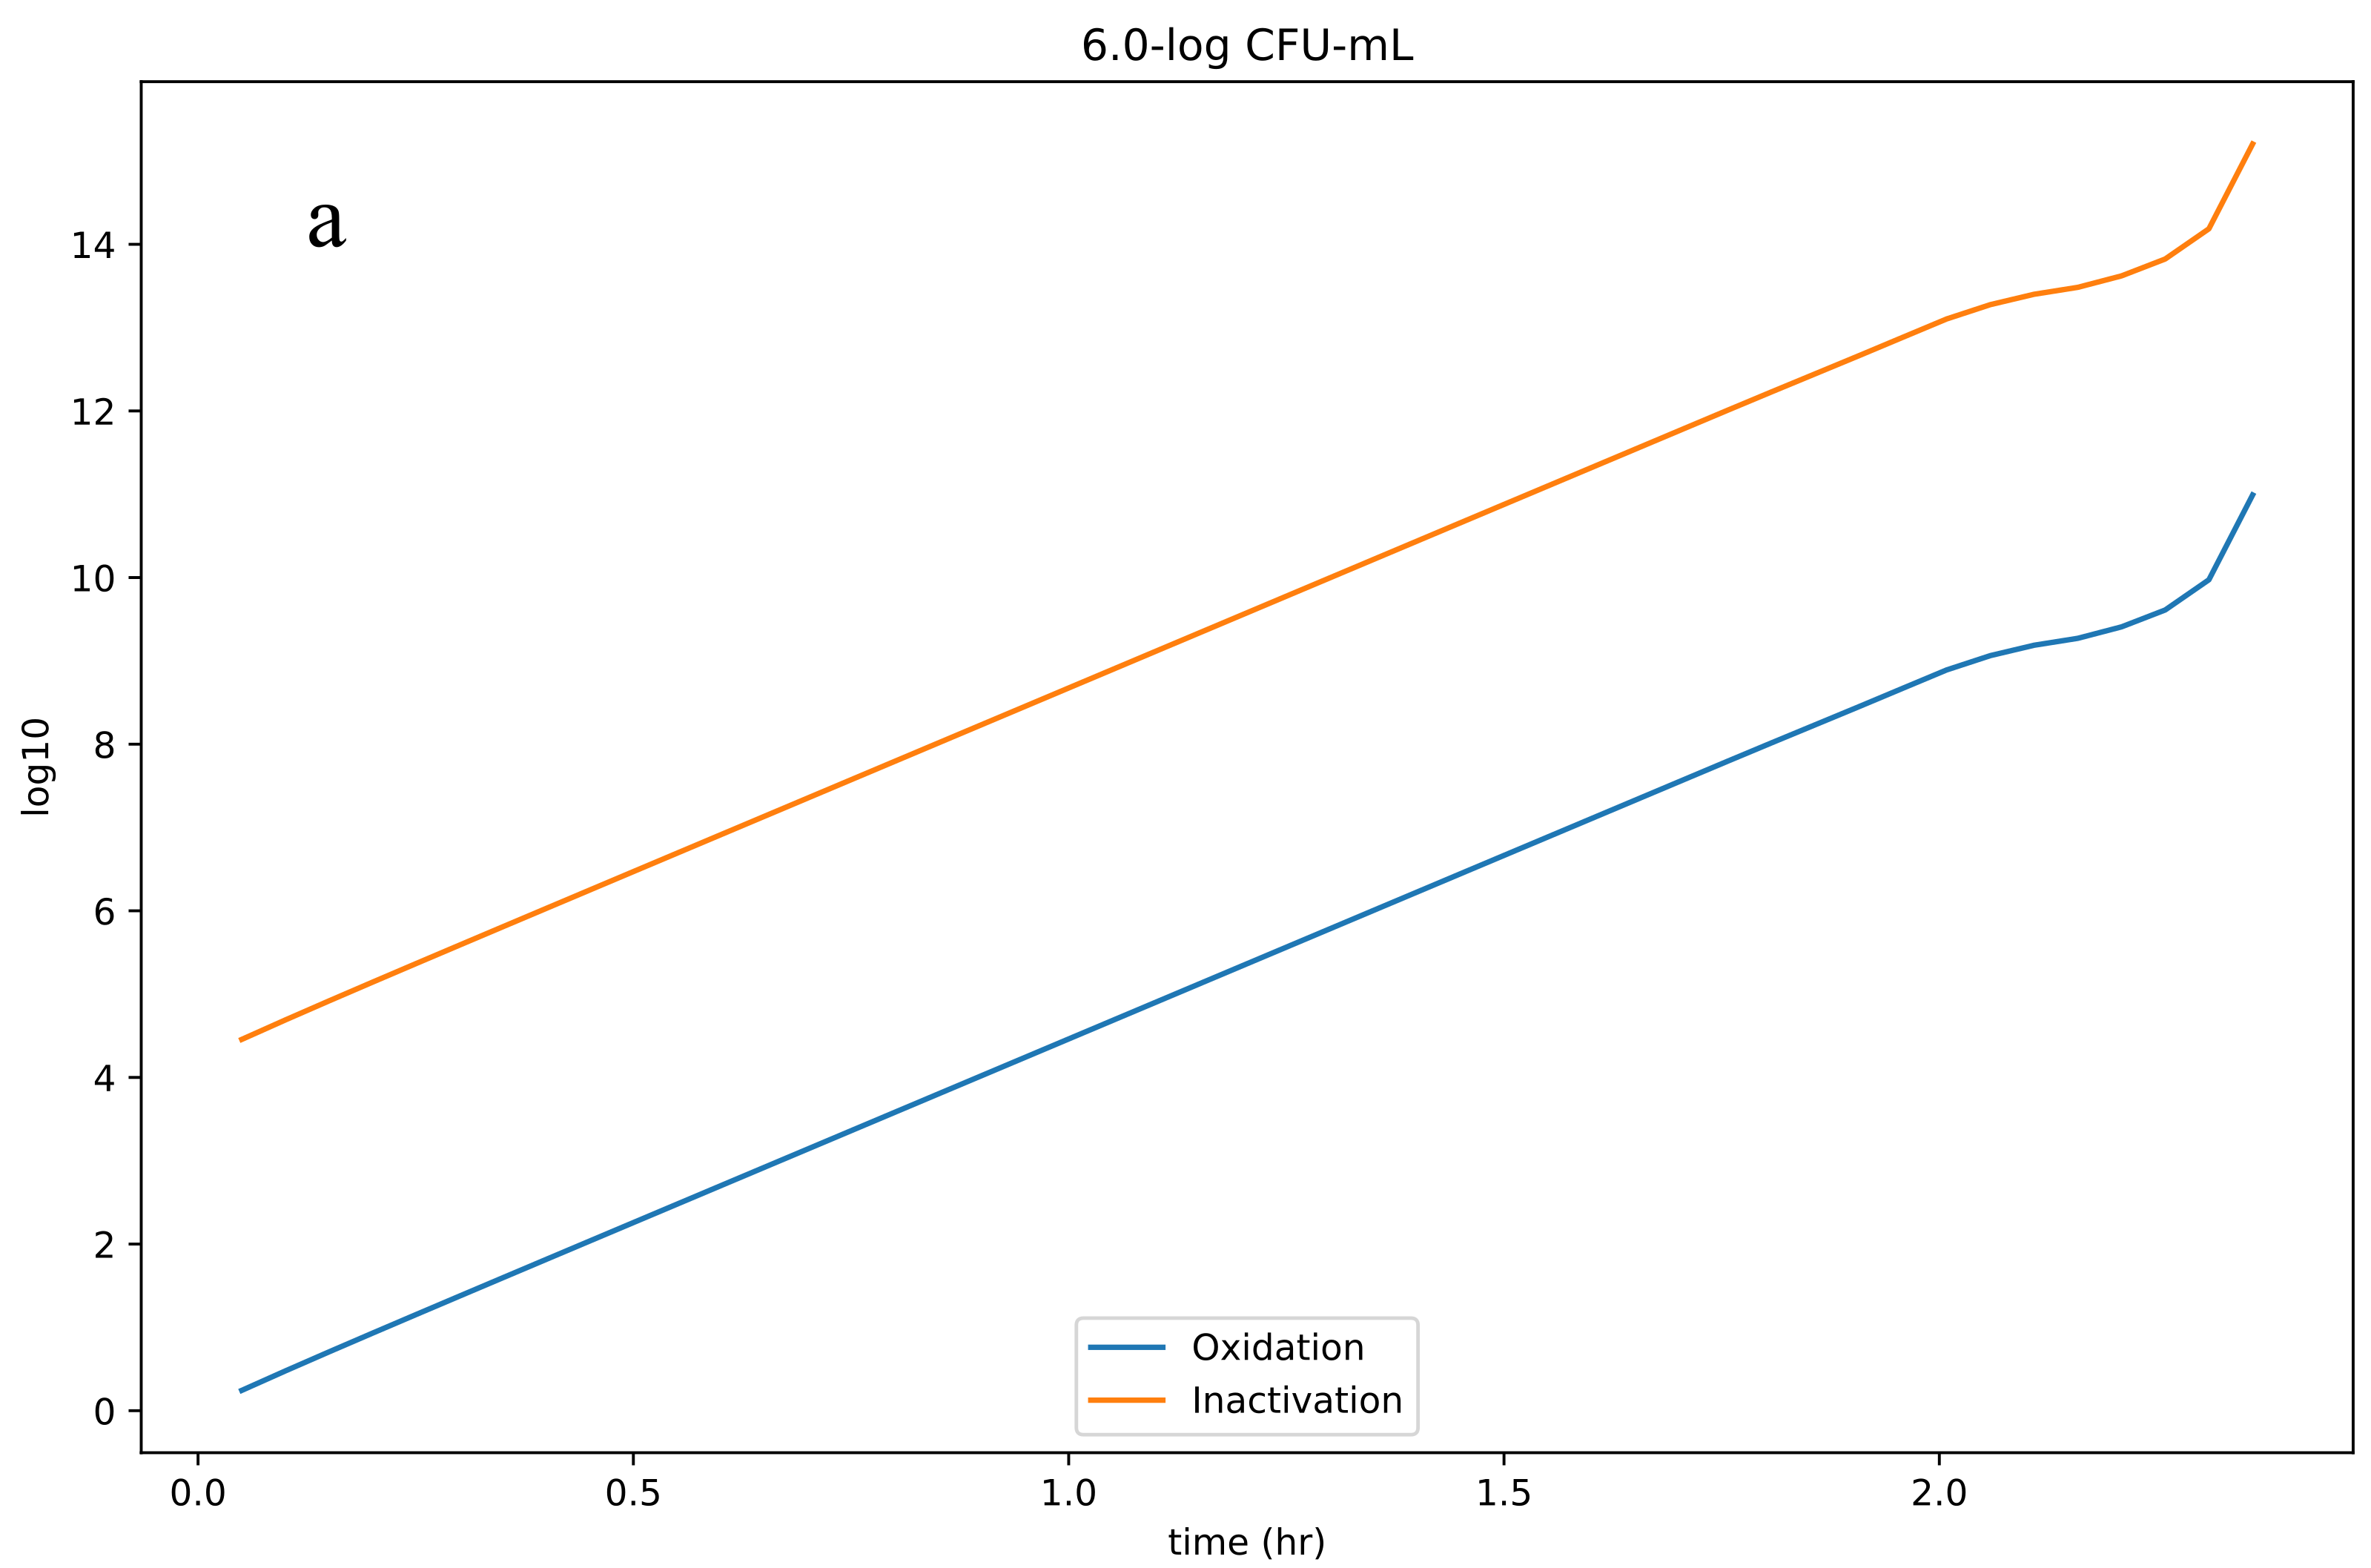
\includegraphics[width = 0.9\textwidth]{images/PDIpy/sensitivity_analyses/bacterial_cfus/6-log_cfu.png} \\
    \vspace{5mm}
    \midrule
    \vspace{5mm}
    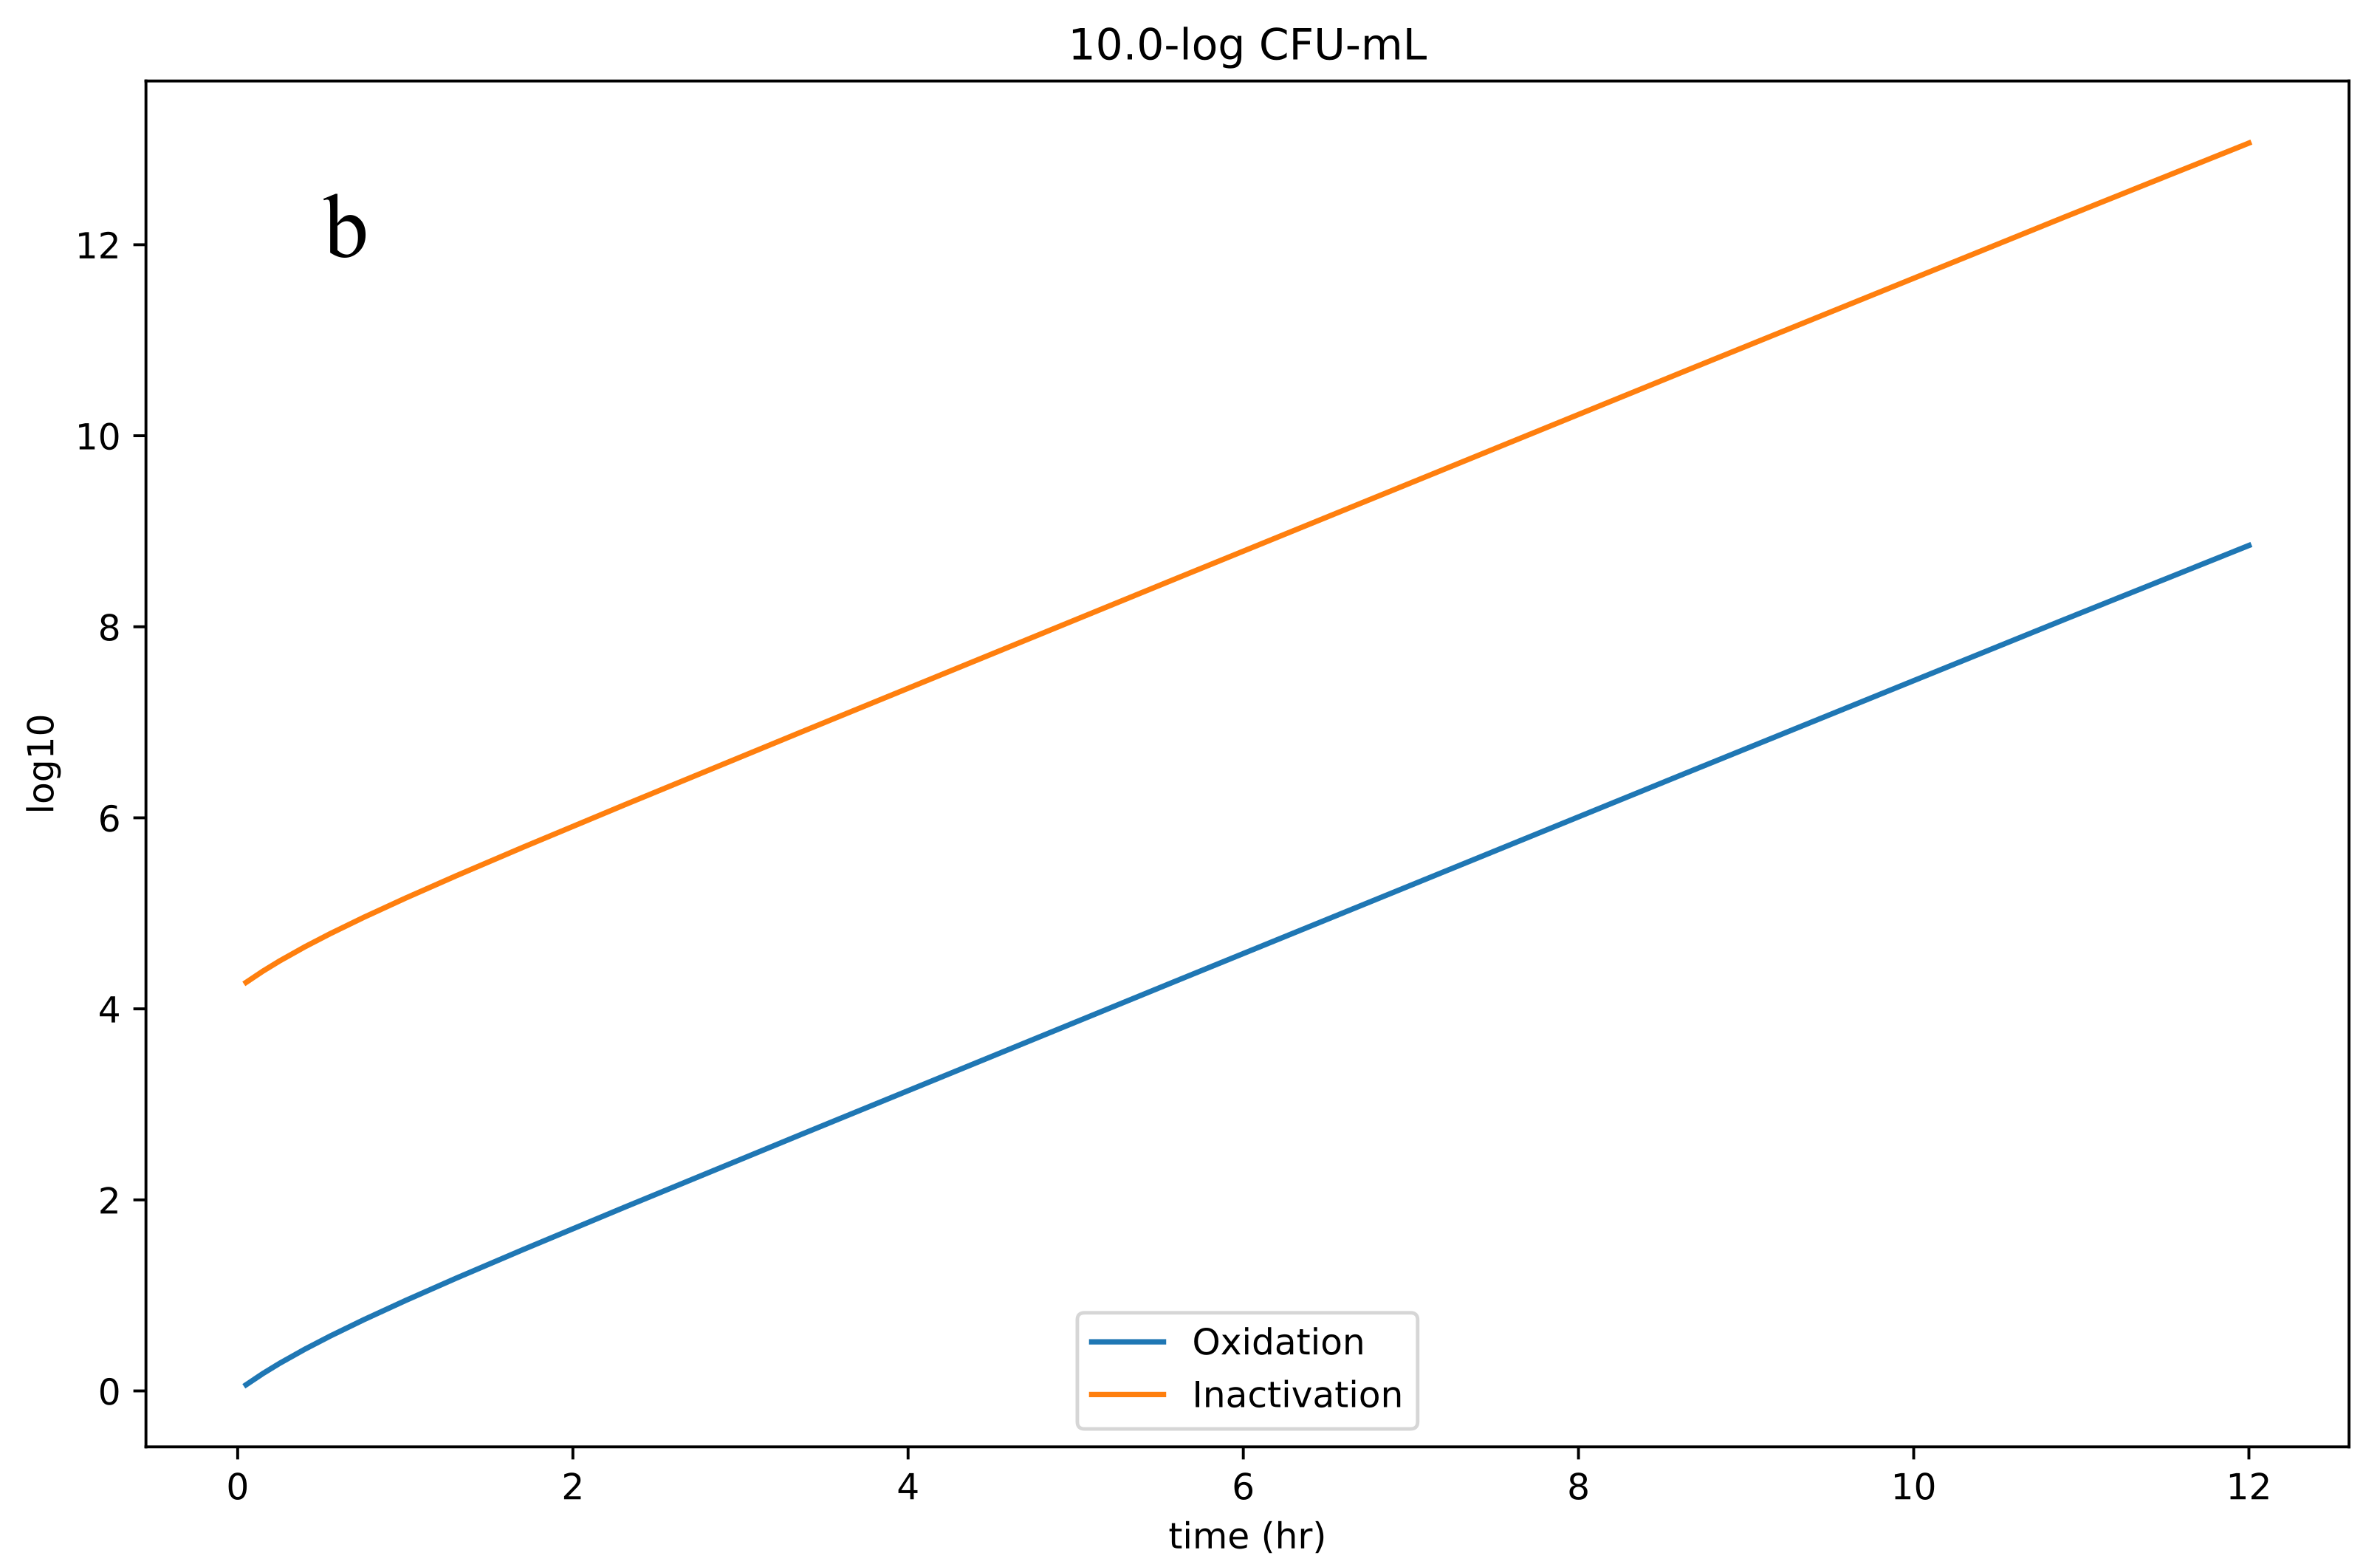
\includegraphics[width = 0.9\textwidth]{images/PDIpy/sensitivity_analyses/bacterial_cfus/10-log_cfu.png}
    \caption{
        A comparison of oxidation and inactivation between a) 1E6 and b) 1E10 $\frac{CFU}{mL}$. The imposed trend is that oxidation and thus inactivation are inversely proportional to the colony size, which is the intuitive result.
    }
    \label{bacterial_cfus}
\end{figure}

\paragraph{Photobleaching constant}
The influence of photobleaching constant was explored over an 8-log range of values, which is depicted in Figure \ref{photosensitizing_constant}. The values below $1E4$ are indistinguishable over time. 

\begin{figure}
    \centering
    \includegraphics[width = 0.9\textwidth]{images/PDIpy/sensitivity_analyses/photobleaching_constant/1E4.png} \\
    \vspace{5mm}
    \midrule
    \vspace{5mm}
    \includegraphics[width = 0.9\textwidth]{images/PDIpy/sensitivity_analyses/photobleaching_constant/1E3.png}
    \caption{
        A comparison of the excitation proportion with two photobleaching constants. Constant values below 1E4 are approximately indistinguishable.
    }
    \label{photosensitizing_constant}
\end{figure}


\subsection{Supplementary figures}
This section includes supplementary figures for the main text. The natural and synthetic porphyrins that inspire the design of photosensitizers are depicted in Figure \ref{zinc_porphyrin}. 

\begin{figure}
    \centering
    \includegraphics[width = \textwidth]{images/PDIpy/background/chlorophyll.png} \\
    \midrule
    \includegraphics[width = 0.5\textwidth]{images/PDIpy/background/zinc_porphyrin.png}
    \caption{
        The chemical structure of porphyrinoid chlorophyll (top) juxtaposed with the core motif of a synthetic porphyrin analogue (bottom). The "R" groups of the synthetic porphyrin can be substituted with a range of functionality to tailor the PS for the specific PDI system.
    }
    \label{zinc_porphyrin}
\end{figure}

% \newpage
% \startchapter{A kinetic model and API of PDI}
\label{PDIpy_chapter}

\section{Introduction}
Antibiotic resistant infections are projected to exceed cancer in annual deaths, and globally cost $10^{13}~USD$ in lost economic production, by mid-21st century \cite{ONeill2014AntimicrobialNations}. Methicillin-resistant \textit{Staphylococcus aureus} (MRSA) \cite{Song2011SpreadStudy,Borg2007PrevalenceCountries} and fluoroquinolone-resistant \textit{Salmonella} \cite{Moghnieh2018EpidemiologyLeague} are two worrisome examples of virulent pathogens that are developing resistance to the antibiotics that subdued them during the 20th century. Antimicrobial resistance (AMR) evolution can be slowed by reducing excessive and incomplete use of antibiotics for human illness and animal agriculture (which is globally the primary consumer of antibiotics \cite{VanBoeckel2017ReducingAnimals,Eggleton2020TheWorld}); however, the fundamental cause of AMR is the conventional strategy of targeting a specific microbial vulnerability. This high selectivity can mitigate off-target effects, however, it places evolutionary pressure on the pathogen to fortify the targeted biochemical vulnerability and thus become immune to the treatement. This arms race of medicinal chemists against microbial evolution must therefore be replaced with a more efficient and sustainable medical strategy, and one that ideally also avoids the persistent ecotoxicity  \cite{Thomas2001AntifoulingEffects,Niu2016RolesIrradiation,Winters1983ControlDesalination}.

\subsection{Photodynamic inactivation}

Photodynamic inactivation (PDI), which differs from photodynamic therapy (PDT) for cancer treatment \cite{Lange2019ComparisonLines} only in its application, offers an effective alternative for treating prokaryotic \cite{Hamblin2004PhotodynamicDisease} and viral \cite{Wigginton2010OxidationInactivation,Lebedeva2020TheViruses} pathogens. PDI describes a photochemical process where reactive oxygen species (ROSs) \cite{Zepp1992HydroxylReaction,Koppenol2001TheLater}, primarily singlet state oxygen ($\ce{^1O2}$, the lowest excitation state of diatomic oxygen) \cite{Ergaieg2008InvolvementPorphyrin, Allen2004IntroductionSimulations, Henze2019Multi-scaleCheckpoint, Zaman2005ComputationalMatrices,Gillespie2007StochasticKinetics}, non-selectively oxidize biological substrate \cite{Choe2006MechanismsOxidation,Frankel1980LipidOxidation}. This mechanism enables PDI to simultaneously 1) avoid resistance evolution \cite{Tavares2010AntimicrobialTreatment,Lauro2002PhotoinactivationConjugates,Pedigo2009AbsenceTherapy}; 2) treat recalcitrant biofilms \cite{Beirao2014PhotodynamicPorphyrin,Ghorbanzadeh2020ModulationModel}, where the biofilm matrix is itself oxidized by $\ce{^1O2}$; and 3) avoid ecological presistence, since $\ce{^1O2}$ has only a $\approx 100 nm$ diffusion distance and a $\approx 10^{-6} s$ lifetime \cite{Moan1984TheOxygen, Moan1990OnTissues,Rodgers1982LifetimeMeasurements} in aqueous environments. The last quality encourages the use of PDI in wastewater treatment \cite{Kohn2007AssociationOxygen,Mostafa2013SingletMatter,Jimenez-Hernandez2006SolarSensitizers} and surfaces \cite{McCoy2014PhotodynamicControl} or industrial polymers \cite{Kim2003DesignProblem} where $\ce{^1O2}$ won't leach into the environment or human consumables. 

The distinction between $\ce{^1O2}$ and triplet state oxygen ($\ce{^3O2}$, the ground conformation of diatomic oxygen) is explained by their quantum multiplicities. The singlet state, of any molecule, contains only paired electrons (couples of electrons with up and down spins) and is named after its multiplicity of $1$: from 
\begin{equation} \label{multiplicity}
    multiplicity = 2(S)+1
\end{equation}
when $S=0$. The $S$ variable in \cref{multiplicity} describes the total angular momentum of the molecule -- the sum of electron spins, where up is $+\frac{1}{2}$ and down is $-\frac{1}{2}$ -- which in the case of a singlet molecule is 0 since the complete pairing of electrons necessitates that the quantities of up and down electrons are equivalent (Figure S1). The molecular triplet state, in contrast, contains two unpaired (radical) electrons that result in a multiplicity of $3$ from $S=1$ in \cref{multiplicity}. These unpaired electrons in $\ce{^3O2}$ increase shielding of the nuclear charges \cite{Katriel1972ARule} and consequently stabilize $\ce{^3O2}$ by $0.98$ eV \cite{Jockusch2008SingletExcitation} relative to $\ce{^1O2}$ that contains lacks this shielding.

The excitation of $\ce{^3O2}$ to $\ce{^1O2}$ is controlled and augmented in PDI by photosensitizer catalysts (PSs). The PS advantageously 1) is a means of localizing oxidation, 2) is a means of controlling the timing and magnitude of excitation; and 3) is a means of generating antimicrobial concentrations of $\ce{^1O2}$ that would not occur by direct excitation $\ce{^3O2 ->[{hv}] ^1O2}$ \cite{Krasnovsky2012PhotochemicalEnvironment}, since the formal selection rules \cite{Bowen1936ForbiddenLines} describe that likely excitations are those which preserve the electronic state: i.e. ground triplet to excited triplet. The $\ce{^3O2}$ could potentially excite to another triplet state and then relax into $\ce{^1O2}$ \cite{Long2003SelectionOxygen}; nevertheless, the PS catalyst accelerates $\ce{^3O2}$ excitation through energy transfers \cite{You2018ChemicalOxygen,Schalk2008Near-infraredTetratolyl-porphyrins,Jockusch2008SingletExcitation}.

The first mechanistic step of PDI describes the ground-state PS ($\ce{^1PS}$) absorbing a photon ($hv$) and entering an excited singlet state ($\ce{^1PS^*}$), according to the selection rules. This excited state then relaxes through intersystem crossing, instead of fluorescing \cite{Kessel1982DeterminantsSpectra}, to an excited triplet state ($\ce{^3PS}$),
\begin{equation} \label{ps_excitation_steps}
    \ce{^1PS <=>[{excitation}][{fluorescence}] ^1PS^* ->[][{intersystem-crossing}] ^3PS}~.
\end{equation}
The second step describes relxation via an energy transfer from $\ce{^3PS}$ to $\ce{^3O2}$, instead of phosphorescence \cite{Mcrae1958Enhancement6}, and thereby generates $\ce{^1O2}$ while regenerating the ground-state $\ce{^1PS}$ catalyst,
\begin{equation} \label{excited_ps_steps}
    \ce{^1 PS <-[{phosphorescence}] ^3 PS ->[^3O2] ^1 PS + ^1O2}
\end{equation}
The combined efficiency of \cref{ps_excitation_steps,excited_ps_steps} is encapsulated in a quantum yield of $\ce{^1O2}$ production \cite{Bakalova2004QuantumPhotosensitizers} ($0\le \Phi_{\ce{^1O2}}\le 1 ~;~ \frac{\ce{^1O2} ~molecules ~produced}{photon ~absorbed}$). The $\ce{^3PS}$ and $\ce{^1O2}$ excited states engage in energy transfers instead of $\ce{^1PS^*}$ and $\ce{^3O2^*}$ since they have longer lifetimes as a consequence of fluorescence being more favorable than phosphorescence. The third step and final of PDI describes $\ce{^1O2}$ reacting with biological substrates through Type II oxidation mechanisms, which are concerted Schenck \cite{Prein1996TheApplications} or Alder-ene \cite{Fernandez-torquemada2012DispersionPlants} reactions that produce organic peroxides \cite{Foote1965ChemistrySelectivity}, as opposed to Type I mechanisms \cite{Bolland1949KineticsOxidation,Farmer1943TheRubber,Grynova2011RevisingAutooxidation} that only affect radical substrates \cite{Litwinienko1999DifferentialEsters}. The Type II mechanism most readily affects allylic positions of unsaturated molecules \cite{Ellison1996ThermochemistryIons,Sehon1950TheRadical}, although, saturated molecules, like those in bacterial phospholipids \cite{ODonnell1985NumericalStaphylococci}, are also oxidized by $\ce{^1O2}$,. 

\begin{figure}[t]
    \centering
    \includegraphics[width = \textwidth]{images/PDIpy/background/jablonski_diagram.png}
    \caption{
        A qualitative Jablonski energy diagram of photosensitization. The initial electronic absorption of a photon ($h\nu$) by $\ce{^3O2}$ forms a $\ce{^3O2}$* molecule, following the selection rules of excitation, which is followed with either fluorescence relaxation or an intersystem-crossing relaxation to form the reactive $\ce{^1O2}$. The singlet $\ce{^1O2}$ molecule either relaxes through phosphorescence or it reacts with an organic substrate to form a peroxide, like the illustrated hydroperoxide with a generic “R” organic group. 
    }
    \label{jablonski_diagram}
\end{figure}

\subsubsection{Photosensitizer}
The $\Phi_{\ce{^1O2}}$ efficiency is primarily dependent upon the chemical structure of the photosensitizer catalyst (PS), notwithstanding minor influence of the chemical conditions \cite{Kruk1998PhotophysicsLuminescence,Kullmann2012UltrafastBisporphyrin}. Two primary inefficiencies of PSs are its propensity to relax through fluorescence or phosphorescence, in Figure \ref{jablonski_diagram}, and to photobleach, where irradiation irreversibly compromises molecular absorptivity \cite{Bonnett2010ChemInformTherapy,Wasser1973TheMetallochlorins}. The functionality and charge of the PS should furthermore optimize its association with the targeted cells \cite{VanDerWal1997DeterminationBacteria,Dickson1989CellSurfaces} and minimize off-target oxidation \cite{Lambrechts2005PhotodynamicMice} and host toxicities \cite{Quishida2016PhotodynamicLight} in medical applications. Material applications of PDI \cite{Peddinti2018PhotodynamicThreat,Gottenbos2001AntimicrobialBacteria}, for applications in either biofouling or sterile medical surfaces, further require that the PS is amenable to permanent surface attachment in a manner that retains material properties \cite{McCoy2014PhotodynamicControl}. 

The PS finally influences the biological targets of PDI. Impermeable PSs, which cannot penetrate a cell, generally oxidize the cytoplasmic membrane \cite{Specht1990DepolarizationAction,Ehrenberg1993ElectricAlterations} instead of cytoplasmic contents \cite{Maisch2004AntibacterialDermatology}. This mechanism, which primarily affects the phospholipid fatty acids in Figure \ref{schenck_mechanism}, manifests in cell death through lysis \cite{Sahu2009AtomicColi,Bertoloni1987RoleCells} and generally affects gram-positive bacteria more than gram-negative bacteria \cite{Lauro2002PhotoinactivationConjugates,Merchat1996Meso-substitutedBacteria} since the latter possess a superficial lipopolysaccharide layer that protects the cytoplasmic membrane. Permeable PSs, by contrast, can penetrate a cell and thus generate $\ce{^1O2}$ within the cytoplasm where cytoplasmic chemicals \cite{Bagchi1979RoleAcriflavine} such as guanine nucleotides \cite{Prat1997Determination9,Devasagayam1991FormationOxygen} are fatally oxidized. This mechanism is more effective with prokaryotes than eukaryotes \cite{Quishida2016PhotodynamicLight}, since the latter have a nuclear membrane that protects DNA, particularly guanine, from oxidation \cite{Pereira2013PhotodynamicVitro}.

A narrow range of chemicals meet these criteria of an ideal PS. Semiconductors \cite{Nelson2002PhotoconductivityDioxide,Peiro2006PhotochemicalPreparations,Linsebigler1995PhotocatalysisResults}, and some amino acid residues \cite{Lippincott-schwartz2003PhotobleachingTechniques,Jin1995PhotolysisSolution}, can electrocatalytically generate $\ce{^1O2}$; however, these molecules are inefficient and/or impractical, particularly for medical applications. The most efficacious PS in nature is chlorophyll \cite{Ramel2012ChemicalPlants}, which is an organometallic porphyrinoid (Figure \ref{zinc_porphyrin}) that evolution has tuned for low rates of photobleaching and absorption of visible light -- specifically blue-violet radiation \cite{Mtangi2017ControlSplitting} via the Soret absorption band \cite{Carre1999FungicidalCerevisiae,Pereira2014InfluencePorphyrin,Ashkenazi2003PhotodynamicBacteria,Moan1986PorphyrinShGroups,Nitzan1992InactivationPorphyrins,Durantini2006PhotodynamicBacteria,Salmon-Divon2004MechanisticTetra-mesoN-methylpyridylporphine} and green-orange radiation \cite{Bertoloni2000PhotosensitizingCells} via the Q absorption band \cite{Bonnett1999PhotobleachingStudy,Jori2006PhotodynamicApplications,Gad2004TargetedMice,Zhao2019Porphyrin-basedAbsorption}. Chlorophyll, however, has not evolved traits that optimize its association with cellular targets or its compatibility with material surfaces; therefore, synthetic porphyrins \cite{Orenstein1997TheInfections,Beirao2014PhotodynamicPorphyrin,Merchat1996StudiesPorphyrins} that emulate the successful conjugated structure \cite{Huang2008Porphyrin-dithienothiopheneCells} of chlorophyll, while introducing other metal centers \cite{Mosinger1997QuantumPorphine} and functional handles  \cite{Hirao1999TheoreticalDerivatives,Wu2014BODIPY-basedSolution,Chacon1988SingletArachidonic} (e.g. Figure \ref{zinc_porphyrin}) that improve its utility in PDI \cite{Jager2016QScales,Karolczak2004PhotophysicalTetraphenylporphyrin,Mathai2007SingletTherapy}, is an appealing direction for PDI research. 

\begin{figure}
    \centering
    \includegraphics[width = \textwidth]{images/PDIpy/background/chlorophyll.png} \\ \midrule
    \includegraphics[width = 0.5\textwidth]{images/PDIpy/background/zinc_porphyrin.png}
    \caption{
        The chemical structure of porphyrinoid chlorophyll (top) juxtaposed with the core motif of a synthetic porphyrin analogue (bottom).
    }
    \label{zinc_porphyrin}
\end{figure}

\begin{figure}[t]
    \centering
    \includegraphics[width =0.9 \textwidth]{images/PDIpy/background/BCFA_schenck_oxidation_2.png}
    \caption{
         The Schenck reaction and associated byproduct decompositions. Step (1) depicts the concerted\cite{Foote1968PhotosensitizedOxygen} Schenck reaction. Step (2) depicts the homolytic cleavage of the hydroperoxide bond to form $\ce{OH^.}$ and an oxy radical that may enter autoxidation mechanisms. Step (3) depicts radical propagation via hydrogen abstraction to form another radical substrate and an alcohol byproduct as part of the autoxidation mechanism. Step (4) is a concerted Russell reaction\cite{Russell1957Deuterium-isotopeRadicals,Howard1968TheMechanism} between two hydroperoxides that forms a $\ce{H2O2}$, an $\alpha,\beta$-ketone, and an alcohol. The reactions of Steps (2-4) sample the wide array of possible oxidative decompositions that follow the Schenck or autoxidation mechanisms.
    }
    \label{schenck_mechanism}
\end{figure}

\subsection{PDI modeling}
Computational models of PDI that allow experimentalists, biologists and chemists alike, to explore the efficacies of different PSs and system conditions are scarce. Santos et al. \cite{Santos2020ApplicationAureus} developed a second-order polynomial to mathematically describe the inactivation of \textit{S. aureus} as a function of time at a particular wavelength and PS concentration. The predictions were demonstrated to be accurate, however, the model is bound to a narrow range of conditions, and does not permit the investigator to explore different parameters such as PS characteristics. Brasel et al. \cite{Brasel2020AnAgalactiae} developed a sigmoidal logistic model to assess the sensitivity of PDI inactivation to incident irradiance $\frac{mW}{cm^2}$ and exposure time; however, the model likewise does not permit investigations of alternative PDI systems. Finally, Sabino et al. \cite{Sabino2019InactivationTherapy} developed a Weibull power-law function from fitted inactivation data to practically predict lethal doses and the tolerance factor of a PDI system; yet, the mathematical model is limited in scope and does not describe the fundamental chemistry of PDI. 

We therefore developed a mechanistically resolved kinetic model of PDI for an impermeable PS and encapsulated into a Python API (PDIpy) that allow investigators to efficiently explore a continuum of values for numerous parameters. The means of editing and customizing the extensive list of parameters, and understanding the default values, is detailed in the API documentation. PDIpy uses Tellurium \cite{Choi2018Tellurium:Biology} to concisely construct SBML \cite{Keating2020Models}, SED-ML \cite{Waltemath2011ReproducibleLanguage}, and COMBINE OMEX \cite{Bergmann2014COMBINEProject} descriptions of the simulations and their results. These conventional formats in computational biology support transparency and reproducibility of the simulation results. The logistic (sigmoidal) Hill equation is then fitted to simulation predictions of cytoplasmic oxidation to systematically construct the inactivation plot based upon the oxidation predictions. We exemplify the model through replicating experimental studies and conducting a sensitivity analyses of key API parameters. We expect that the open-source project will foster experimental progress without expending resources, and will inspire computational biologists to refine tools for this field of medical research, towards expediting the scientific response to the looming medical crisis of antibiotic resistance. 

\section{Methods}
\subsection{Conceptual model}
PDIpy conceptually represents an experimental PDI system with a coccus (spheroid) bacterium like \textit{S. aureus}. Each simulation accepts parameters for each aspect of PDI: the light source and incident intensity; the PS absorptivity, structural dimensions, and $\frac{mol}{vol}$ or $\frac{mol}{area}$ concentration; the bacterial specie, membrane composition, and $\frac{CFU}{mL}$ for planktonic experiments; the solution dimensions; and kinetic constants for the PDI reactions. Default values for many of these parameters supplement user-defined parameters.

\subsection{Kinetic reactions}
Our model is predicated upon a set of three chemical processes that embody the essence of PDI. 1) A photoelectric interaction \cite{Wheaton2009PhotoelectricEffect} from \cref{ps_excitation_steps} occurs after $\ce{^1PS}$ is struck by a photon ($h\nu$) and undergoes intersystem crossing per to form $\ce{^3PS}$. 2) An energy transfer in \cref{excited_ps_steps} occurs from $\ce{^3PS}$ to $\ce{^3O2}$. 3) The $\ce{^1O2}$ oxidizes biological substrates, which includes both cytoplasmic phosholipids and biofilm polymeric substances, or it irreversibly disrupts PS absorptivity through photobleaching 
\begin{equation} \label{bleaching}
    \ce{^1PS -> ^1PS_{bleached}}~.
\end{equation}
A complete description of this kinetic system is represented in Table \ref{reactions_table}, and each of the reactions are each detailed in the following sub-sections.

\subsubsection{User inputs}
The PDIpy API accepts a variety of parameters that allow the user to customize almost every aspect of the PDI system. These parameters of the simulated PDI system can be provided through either a dictionary argument in the \pyobject{define\_conditions} function, or through a JSON parameter file for each category of parameters -- e.g. light, PS, bacterium, and solution space -- that elaborate the simulated system in a more reproducible and transparent manner than dictionary arguments. The complete list of accepted parameters and formats are detailed in the PDIpy documentation (\url{https://github.com/freiburgermsu/PDIpy/blob/main/README.rst}).

\begin{table}[]
    \centering
    \begin{tabular}{c|c}
        \textbf{Name} & \textbf{Reaction} \\
        \toprule
        Photoexcitation & \ce{^1PS <=> ^3PS} \\
        Photobleaching & \ce{^1PS -> ^1PS_{bleached}} \\
        Energy transfer & \ce{^3PS + ^3O2 -> ^1PS + ^1O2} \\
        Phosphorescence & \ce{^1O2 -> ^3O2} \\
        Membrane oxidation & \ce{^1O2 + FA -> oFA} \\
        EPS oxidation & \ce{^1O2 + EPS -> oEPS} \\
    \end{tabular}
    \caption{
        Each of the chemical reactions that define the PDI model of PDIpy. These reactions are individually detailed in dedicated subsections.
    }
    \label{reactions_table}
\end{table}

\subsubsection{Photoelectric}
\paragraph{PS excitation}
PDI begins with the excitation of the PS. This occurs as the combined result of an incident photon i) entering the aqueous solution, ii) striking a PS, and then iii) exciting an electron. This sequence is encapsulated in the kinetic expression
\begin{multline} \label{ps_excitation_kinetics}
    \frac{d[\ce{^3PS}]}{dt} =  k_{excitation}*\frac{photons_{PS}}{photons_{total}} \\ 
    *\Phi_{excitation}*[\ce{^1PS}] - k_{fluorescence}*[\ce{^3PS}]~. 
\end{multline}
The $k_{excitation}$ \& $k_{fluorescence}$ rate constants are estimated as the inverse of the rise and decay times for the selected PS, respectively. The approximate rise time for a porphyrin PS is $50 fs$, which is consistent with estimates of $<100 fs$ \cite{Andersson1999PhotoinducedState} and $60-90 fs$ in ethanol solvent \cite{Gurzadyan1998Time-resolvedZn-tetraphenylporphyrin} which elongates the lifetime of excited molecules relative to water. The decay time, as the S2 fluorescence \cite{Akimoto1999UltrafastPorphyrins}, and $\Phi_{excitation}$ ($\frac{PS excited}{photon absorbed}$) are approximated for a porphyrin PS as $1.5 ns$ and $\approx 0.7$ \cite{Krasnovsky2012PhotochemicalEnvironment}, respectively. The $\frac{photons_{PS}}{photons_{total}}$ \cite{Brasel2020AnAgalactiae}, which is the proportion of photons in the solution that strike a photosensitizer, is calculated through a series of steps. 1) The reported intensity of incident light from the respective light source -- i.e. either irradiance ($\frac{mW}{cm^2}$), lux ($\frac{lumen}{m^2}$), or lumens (lumens) -- is converted into $watts_{incident}$ ($\frac{J}{s}$). 2) This wattage is attenuated by the proportion of the emission spectrum $light_{incident}$ that resides within the excitation spectrum of the parameterized photosensitizer $light_{excitation}$, 
\begin{equation}
    watt_{excitation} = \frac{light_{excitation}}{light_{incident}}*watts_{incident}.
\end{equation}
3) The $watt_{excitation}$ is used to calculate the moles of incident photons that strike photosensitizers per timestep 
\begin{multline} \label{photons_per_second}
    \frac{photons_{PS}}{timestep}=\frac{<h\nu_{excitation}>}{h*c}*watts_{excitation} \\
    *\frac{second}{timestep}*reflection*scattering*\frac{1 mole}{N_A}*\frac{vol_{PS}}{vol_{total}},
\end{multline}
where $reflection \approx 96 \%$ represents the proportion of incident photons that penetrate an aqueous solution \cite{Gross1993SingletLiposomes}; and $scattering$ represents the proportion of light that reaches a specified depth \cite{RobertW.1973TheSea}, which is calculated by 
\begin{equation}
    I_z = I_0*e^{-k*z}~,
\end{equation}
where $I_z$ is the light intensity relative to the $I_0$ after depth $z$, and $k$ is the attenuation coefficient, which is $\approx 0.04~(\frac{1}{m})$ \cite{Lorenzen1972ExtinctionPhytoplankton} for clear waters. The $\frac{vol_{PS}}{vol_{total}}$ represents the volume proportion of the PS ($vol_{PS}$) -- calculated as the product of the quantity of PS molecules and the volume per molecule per its structure -- to the total volume of the solution in which the PS resides ($vol_{total}$) \cite{Santos2020ApplicationAureus}. The average excitation wavelength of the PS ($<h\nu_{excitation}>$) is calculated as the weighted average of the Soret and Q excitation bands, in proportion to their relative contribution in generating $\ce{^1O2}$ \cite{Nitzan2001PhotoinactivationWavelengths,Hoenes2020PhotoinactivationWavelength}, since this averaged wavelength simultaneously embodies contributions of both excitation bands. The resultant $\frac{photons_{PS}}{timestep}$ from \cref{photons_per_second} is then divided by the $\frac{photons_{total}}{timestep}$ to complete the kinetic expression in \cref{ps_excitation_kinetics} that calculates the excitation of PS in each timestep. 

\paragraph{Photobleaching}
The collision of a PS and a photon may alternatively disrupt the conjugated PS system and prevent further excitation, which is depicted in \cref{bleaching}. The kinetic expression 
\begin{equation} \label{bleaching_kinetics}
    \frac{d[\ce{^1PS_{bleached}}]}{dt} = k_{bleaching}*[\ce{^1PS}]*[\ce{^1O2}]~,
\end{equation}
represents this process. The $k_{bleaching}$ rate constant for the oxygen-dependent photobleaching reaction of \cref{bleaching_kinetics} -- as opposed to the oxygen-independent, first-order, photobleaching reaction \cite{Bonnett1999PhotobleachingStudy,Mang1987PhotobleachingTherapy} -- possesses a rate constant of $\approx 600 \frac{cm^2}{J*M}$ \cite{Dysart2005CalculationCells} for porphyrins, which is a function of light exposure $\frac{J}{cm^2}$.

\subsubsection{Energy Transfer}
The energy transfer from $\ce{^3PS}$ to $\ce{^3O2}$  in \cref{excited_ps_steps} is described with by the kinetics expression
\begin{equation} \label{energy_transfer_kinetics}
    \frac{d[\ce{^1O2}]}{dt} = k_{transfer}*\Phi_{transfer}*[^3PS]*[\ce{^3O2}]. 
\end{equation}
The rate constant $k_{transfer}$ is the inverse of the decay time of $\ce{^3PS}$, which for a porphyrin PS appears to be $100 ns$ in aqueous after accounting for the reported value \cite{Kupper2002KineticsOxygen} in acetone solvent that significantly increases the lifetime of excited states \cite{Spikes1992QuantumUroporphyrin}. The $\ce{^1O2}$ phosphorescence side reaction, which often emits a specific infrared wavelength that can be measured to approximate the $[\ce{^1O2}]$ \cite{Macpherson1993DirectCentres}, is kinetically represented 
\begin{equation}
    \frac{d[\ce{^3O2}]}{dt} = k_{phosphorescence}*[\ce{^1O2}]
\end{equation}
where $k_{phosphorescence}$ is a function of $\frac{CFU}{mL}$, since the $\ce{^1O2}$ lifetime is greater in biological material and thus it is proportional with the bacterial concentration in planktonic simulations \cite{Maisch2007TheBacteria}. The minimum lifetime is limited to $3.5\mu s$ for pure water \cite{Baier2005Time-resolvedCells}.

\subsubsection{Oxidation}
The oxidation reactions are the primary consumers of oxygen in the kinetic system. The simulated system, however, is assumed to possess an equilibrium between the solution and the atmosphere, which prevents the depletion of oxygen in the system. This is represented by replacing each oxygen molecule that is consumed during the oxidation of biological substrate in \cref{membrane_oxidation,EPS_oxidation}.

\paragraph{Cytoplasmic membrane} 
The oxidation of cytoplasmic phospholipids, which we approximate as fatty acid chains, is represented as an irreversible second-order reaction \cite{Watabe2007OxidationMembranes.}
\begin{equation} \label{membrane_oxidation}
    \ce{^1O2 + FA -> oFA}.
\end{equation}
and a second-order kinetic expression
\begin{equation} \label{membrane_oxidation_kinetics}
    \frac{d[oFA]}{dt} = k_{fa}*[\ce{^1O2}]*[FA]~.
\end{equation}
The rate constant $k_{fa} \approx 769 \frac{L}{g*s}$ \cite{Mukai2019KineticSolution} and the concentration of fatty acid chains in the cytoplasmic membrane is described in units of $\frac{g}{L}$, after calculating the weighted average MW of fatty acids within the membrane. 

\paragraph{Biofilm matrix} 
The oxidation of EPS is reported to be significant during PDI \cite{Beirao2014PhotodynamicPorphyrin}. This process is represented through an irreversible reaction
\begin{equation} \label{EPS_oxidation}
    \ce{^1O2 + EPS -> oEPS},
\end{equation}
which competes with \cref{membrane_oxidation} for $\ce{^1O2}$ and thereby lessens the efficacy of PDI upon biofilms relative to planktonic organisms. The oxidation of bioiflm polymers is kinetically represented  
\begin{equation} \label{EPS_oxidation_kinetics}
    \frac{d[oEPS]}{dt} = k_{EPS_{oxidation}}*[\ce{^1O2}]
\end{equation}
with an empirical rate constant that we approximated as $37.75~\frac{1}{s}$ for \textit{S. aureus}, and an initial concentration of EPS that is $9x$ greater than the cellular mass, in proportion to mass distributions of biofilms \cite{Flemming2010TheMatrix}.

\subsection{Inactivation fitting}

Simulation results of chemical concentrations over time are processed into predictions of bacterial inactivation through a series of mathematical steps. 1) The proportion of oxidized substrate
\begin{equation} \label{oxidation_proportion}
    ox_{proportion} = \frac{[oFA]}{[oFA]+[FA]}
\end{equation}
is fitted to a sigmoidal curve, similar to other models \cite{Xiong1999AInactivation}. We used the signmoidal Hill-equation \cite{Gesztelyi2012ThePharmacology} as a biochemical kinetic model that derives from mass-action kinetics similar to the Michaelis-Menten kinetic model, however, a fitting module for the Hill-equation did not exist; hence, the HillFit Python module was developed with a variation of the Hill-equation \cite{Inoue2016OscillationActivation} 
\begin{equation} \label{hill_eq}
    y=bottom+\frac{(top-bottom)*x^n}{EC50^n+x^n}~,
\end{equation}
that improves its fit to data, to fit the oxidation data from PDIpy simulations. The regression parameters from the fitted Hill equation are then systematically adjusted to construct an inactivation plot that replicates experimental results while preserving the underlying Hill-equation relationship. These parameter adjustments are presented in Table \ref{hill_parameters} for both simulations of planktonic and biofilm bacteria, since biofilms factors such as impaired diffusion that are not explicitly accounted in our kinetic model and thus must be compensated through other means. The top parameter of \cref{hill_eq} is adjusted asymptotically to a limit that follows an subtly different empirical expression for planktonic $1-10^{-\Omega}$ than biofilm $1-10^{-0.7-\Omega }$ simulations, where $\Omega = wattage^{\frac{1}{5}}-log10(1-final_{oxidation\_proportion})$. This top limit is empirically determined to manifest in the log-inactivation predictions being 1-2 greater than the log-oxidation from \cref{oxidation_proportion}, which embodies our assumption -- and an implicit observation in experimental studies -- that $1-10\%$ of membrane phospholipids must experience oxidation for the cell to lyse. 

\begin{table}[]
    \centering
    \begin{tabular}{l|c|c}
        \textbf{Bacterial state} & \textbf{Hill parameter} & \textbf{Adjustment} \\
        \multirow{2}{}{Planktonic} & EC50 & -76\% \\
         & nH & +100\% \\
         \midrule
         \multirow{2}{}{Biofilm} & EC50 & -65\% \\
         & nH & +120\% \\
    \end{tabular}
    \caption{
        The Hill parameters adjustments that are enacted to create the inactivation plot for both planktonic and biofilm systems. 
    }
    \label{hill_parameters}
\end{table}

% \subsubsection{Cross-linked systems}

% \paragraph{iPDIpy}
% The PDIpy API is graphically interactive through a user interface iPDIpy, which is depicted in Figure \ref{}. This interface provides a convenient means for parameterizing a PDIpy simulation, exporting and importing sets of parameters, parsing the processed simulation data, viewing error messages and calculated values, viewing the output figure of bacterial reduction over time, and parsing the processed data through a build-in function. The iPDIpy version of PDIpy is downloadable from our GitHub repository.

% \begin{figure}
%     \centering
%     \includegraphics{}
%     \caption{
%         The left pane of the GUI will contain command buttons like restarting the simulation or export results, while the right pane will edit the simulation data and or bacterial qualities/species.
%     }
%     \label{iPDIpy_interface}
% \end{figure}


\section{Case Studies}
A PDI experiment from literature that thoroughly described its expeirmental procedure was parameterized in PDIpy to compare the predicted results with the reported results. These comparisons in the following sections all pertain to \textit{S. aureus}, which is a model coccus bacterium that is abundantly described in studies of PDI and AMR infectants as MRSA.

% \subsection{Cross-linked PS}
% Experimental data from our lab with cross-linked PSs (unpublished) was parameterized, in Table \ref{}, into PDIpy. The predicted reduction curve over time in Figure \ref{} agreed with the experimental data at the measured time of 6 hours and 98\% reduction, which supports that the software yields accurate predictions. 

% \paragraph{}
% .

\subsection{Solution PS}

\paragraph{Beirao et al.\cite{Beirao2014PhotodynamicPorphyrin}}
This paper experimentally examines the efficacy of a dissolved PS, over a range of concentrations, against both planktonic and sessile states. The ample experimental details were parameterized into PDIpy, and the predicted log-inactivation was contrasted with the reported log-inactivation at various times, concentrations, and bacterial states in Table \ref{beirao_et_al_data}. The predicted log-oxidation and log-inactivation for a few of the simulated conditions from the study are plotted in Figure \ref{beirao_et_al}, with the respective regression plots from fitting the Hill-equation to the log-oxidation results in Figure \ref{hill_regression}. The very precise fitting of the data -- $R^2 > 0.996$ -- supports that our kinetic model of PDI fundamentally recreates the biochemical relationship that is predicted by the Hill model of kinetics.

\begin{table}[h]
    \centering
    \begin{tabular}{c|c|c|c|c|c}
        Bacterial & [PS] & Inactivation & Reported & Predicted & \multirow{2}{1.2cm}{\%-error}\\
        state & ($\mu m$) & (-log10) & (min) & (min) & \\
        \toprule
        \multirow{3}{1.5cm}{planktonic} & 5 & 7.6 & 51 & 117 & 119\\
        & 10 & 7.6 & 51 & 36 & -29\\
        & 20 & 7.6 & 42 & 12 & -71\\
        \midrule
        \multirow{3}{1.5cm}{sessile} & 5 & 3.6 & 390 & 566 & 45\\
        & 10 & 5 & 390 & 310 & -20\\
        & 20 & 6.3 & 390 & 247 & -37\\
        \bottomrule
    \end{tabular}
    \caption{
        A quantitative comparison of published inactivation data, with both planktonic and sessile, \textit{S. aureus}, with predictions from PDIpy. The \%-error for each prediction is provided in the table as a metric of accuracy
    }
    \label{beirao_et_al_data}
\end{table}

\begin{figure}
    \centering
    \includegraphics[width = 0.9\textwidth]{images/PDIpy/examples/20uM.png}
    \vspace{5mm}
    \midrule
    \vspace{5mm}
    \includegraphics[width = 0.9\textwidth]{images/PDIpy/examples/10uM_biofilm.png}
    \caption{
        Two exemplary figures of PDIpy replications of the Beirao et al. data for a) planktonic and b) biofilm bacterial states.
    }
    \label{beirao_et_al}
\end{figure}

\begin{figure}
    \centering
    \includegraphics[width = 0.9\textwidth]{images/PDIpy/examples/20uM_regression.png}
    \vspace{5mm}
    \midrule
    \vspace{5mm}
    \includegraphics[width = 0.9\textwidth]{images/PDIpy/examples/10uM_biofilm_regression.png}
    \caption{
        The Hill-equation regression of the oxidation plot from Figure \ref{beirao_et_al}a. The high $R^2$ correlation supports that our chemical model of PDI is a sensible recreation of the fundamental biochemistry.
    }
    \label{hill_regression}
\end{figure}


\section{Sensitivity analyses}

\paragraph{Light intensity}
The sensitivity of simulation results to light intensities, across the range of $[10, 100,000] Lux$, was explored. The trend over this 3-log range, which is represented by Figure \ref{light_intensities}, is that the proportion of excited PS asymptotically approches 100\%. The influence of photobleaching appears to be negligible at the examined time length and light intensity, where a negative slope in the plotted excitation proportion would be expected over time as a decreasing proportion of PSs are able to electronically excite. The analysis further clarifies the minmal value of greater irradiation beyond $\approx 13,000 lux$ from the perspective of exciting PSs, which may be an informative for experimentalists when designing PDI systems.

\begin{figure}
    \centering
    \includegraphics[width = 0.8\textwidth]{images/PDIpy/sensitivity_analyses/215_lux.png} \\
    \vspace{5mm}
    \midrule
    \vspace{5mm}
    \includegraphics[width = 0.8\textwidth]{images/PDIpy/sensitivity_analyses/100000_lux.png}
    \caption{
        The proportion of excited PS at two contrasting light intensities: a) $215 Lux$ and b) $100000 Lux$. The negative slope of the plots is the consequence of photobleaching, where the quantity of excitable PSs decreases over time. This effect is more prominent in b) since the light intensity is much greater than a), and since photobleaching is a function of light intensity.
    }
    \label{light_intensities}
\end{figure}

\section{Discussion}
The preliminary examples of PDIpy with the study from Beirao et al. support that the underlying kinetic model sufficiently represents PDI. The excessive breadth in the simulation predictions, where the log-inactivation predictions with low concentrations occurs too late while the log-inactivation predictions with high concentrations occurs too early, may be resolved with adjusted the Hill parameters that are defined in Table \ref{hill_parameters}. The tighter spread of the biofilm simulation relative to the planktonic simulation supports this method of improving the predicted results, where the different set of parameter adjustments may be better tailored to inactivation phenomena. 

The sensitivity analysis of the light intensity revealed that the relationship between the proportion of PS excitation and the light intensity plateaus beyond $\approx 10,000 lux$. This insight and this type of broad inquiry over a range of values cannot be replicated with existing PDI models, since they neither consider the fundamental kinetics that results in PS excitation nor are encapsulated in a dynamic interface like the PDIpy API.  

The open-source implementation of this model in PDIpy will practically support experimentalists as they develop PDI technologies, and will ideally inspire other computational biologists to develop programs that can foster discovery of antibiotic methods at an imperative time to prevent antimicrobial resistant epedemics.   


\section{Author Contributions}
\begin{description}
    \item[APF] Designed, executed, and codified the project.
    \item[JRK] Guidance and manuscript edits.
    \item[HLB] Guidance, manuscript edits, and funding.
\end{description}

\section{Acknowledgments}

The authors are grateful to Ethan Sean Chan for his development of the framework for iPDIpy, which will be introduced in a future release of PDIpy. The authors thank the members of the Buckley and Wolff Groups at the University of Victoria for contributing ideas and data that were used to refine this PDI model. Andrew finally thanks Hiroaki Imoto for his contributions and guidance in developing the HillFit module that was used to fit data in PDIpy.
% \newpage
% \subsection{Supporting Information: PDIpy}

\subsection{Molecular properties and mechanisms}
The electronic difference between $^1\Delta_g$ and $^3\Sigma_g^-$ is best depicted through their respective molecular orbital diagrams in Figure \ref{mo_diagrams}. The photochemical processes of $^1\Delta_g$ generation are depicted in Figure \ref{jablonski_diagram}, while the subsequent oxidation reactions are sampled in Figure \ref{schenck_mechanism}.

\begin{figure}
    \centering
    \begin{tabular}{c|c}
        \includegraphics[width = 0.48\textwidth]{images/PDIpy/background/triplet_mo_diagram.png}
        & \includegraphics[width = 0.48\textwidth]{images/PDIpy/background/singlet_mo_diagram.png}
    \end{tabular}
    \caption{
        Qualitative orbital diagrams for a) $^3\Sigma_g^-$ and b) $^1\Delta_g$ configurations of diatomic oxygen. Each barbed arrow represents a single electron, and each platform represents the electronic sub-orbital of the respective label, where orbital energy increases vertically in the diagram. The distinction between a) and b) is highlighted by the red circled electrons and labels, where $^1\Delta_g$ possesses an anti-bonding $\pi^*$-bond in its HOMO that destabilizes it relative to $^3\Sigma_g^-$.
    }
    \label{mo_diagrams}
\end{figure}

\begin{figure}[t]
    \centering
    \includegraphics[width = \textwidth]{images/PDIpy/background/jablonski_diagram.png}
    \caption{
        A qualitative Jablonski energy diagram of Steps b-c of PDI. The initial excitation in PDI occurs via an energy transfer $\ce{^3\Sigma_g^- ->[energy transfer] ^1\Delta_g}$. The ROS then, while abstaining from phosphoresce, oxidizes a biological substrate to form a peroxide that gradually compounds to cause lysis.
    }
    \label{jablonski_diagram}
\end{figure}

\begin{figure}[t]
    \centering
    \includegraphics[width = \textwidth]{images/PDIpy/background/BCFA_schenck_oxidation_2.png}
    \caption{
         The reaction mechanisms of Type II oxidation and subsequent decompositions. \textbf{Step (1)} depicts the concerted \cite{Foote1968PhotosensitizedOxygen} Schenck reaction. \textbf{Step (2)} depicts the homolytic cleavage of the hydroperoxide bond to form $\ce{OH^.}$ and an oxy radical that may enter autoxidation (Type I oxidation) mechanisms. \textbf{Step (3)} depicts radical propagation via hydrogen abstraction to form another radical substrate and an alcohol byproduct. \textbf{Step (4)} is a concerted Russell reaction \cite{Russell1957Deuterium-isotopeRadicals,Howard1968TheMechanism} between two peroxides that forms a $\ce{H2O2}$, an $\alpha,\beta$-ketone, and an alcohol. The reactions of Steps (2-4) sample the wide range of possible decompositions that follow oxidation mechanisms.
    }
    \label{schenck_mechanism}
\end{figure}

\subsection{Excitation proportion} \label{excitation_proportion_estimate}

The steps for estimating the absorbed proportion of incident photons by photosensitizers, where absorbance or transmittance measurements are not available, are detailed through the following steps. a) The reported intensity of incident light from the respective light source -- i.e. irradiance ($\frac{mW}{cm^2}$), lux ($\frac{lumen}{m^2}$), or lumens (lumens) -- is converted into a quantity of incident watts $watts_{in}$ ($\frac{J}{s}$). b) This incident wattage is attenuated by the proportion of the emission spectra $spec_{em}$ that resides within the $spec_{ex}$ of the PS, 
\begin{equation}
    watt_{ex} = \frac{spec_{ex}}{spec_{em}}*watts_{in}.
\end{equation}
c) The $watt_{ex}$ is then used to calculate the moles of incident photons that strike photosensitizers per timestep 
\begin{multline} \label{photons_per_second}
    \frac{photons_{strike~PS}}{timestep}=\frac{<h\nu_{ex}>}{h*c}*watts_{ex} *\frac{s}{\Delta t}*reflection*scattering*\frac{1~mole}{N_A}*\frac{vol_{PS}}{vol_{total}},
\end{multline}
where $reflection \approx 96 \%$ and represents the proportion of incident photons that penetrate an aqueous solution \cite{Gross1993SingletLiposomes}; and $scattering \left(\frac{I_z}{I_0} = e^{-k*z}\right)$ represents the proportion of light $\frac{I_z}{I_0}$ that reaches a specified depth $z$ \cite{RobertW.1973TheSea}, where $k$ is the attenuation coefficient that is $\approx 0.04~(\frac{1}{m})$ \cite{Lorenzen1972ExtinctionPhytoplankton} for clear water. The quotient $\frac{vol_{PS}}{vol_{total}}$ describes the fraction of the solution volume where the PS resides ($vol_{total}$) that is comprised of the PS per se ($vol_{PS}$), which is calculated as the product of the quantity of PS molecules and the volume per molecule according to its molecular structure. The average excitation wavelength of the PS ($<h\nu_{excitation}>$) is calculated as the weighted average of the Soret and Q excitation bands, in proportion to their relative contribution in generating $^1\Delta_g$ \cite{Nitzan2001PhotoinactivationWavelengths,Hoenes2020PhotoinactivationWavelength}, which assumes that both excitation wavelengths are excited during the simulation. The resultant $\frac{photons_{strike~PS}}{timestep}$ from \cref{photons_per_second} is then divided by the quantity of photons that enter the system per timestep $\frac{photons_{total}}{timestep}$ to determine which fraction of photons strike a photosensitizer. 

\subsection{Deduction of inactivation via the Hill equation}

Inactivation may alternatively be deduced from oxidation through parameter manuipulation of a fitted sigmoidal curve, similar to other models \cite{Xiong1999AInactivation}. The Hill-equation \cite{Gesztelyi2012ThePharmacology} is a sigmoidal model that derives from mass-action kinetics, similar to the Michaelis-Menten kinetic model, and thus it was selected the signmoidal model for this alternative framework. A Python program for fitting the Hill-equation was developed -- the HillFit module -- with a variation of the Hill-equation \cite{Inoue2016OscillationActivation} 
\begin{equation} \label{hill_eq}
    y=bottom+\frac{(top-bottom)*x^n}{EC50^n+x^n},
\end{equation}
that introduces an additional $bottom$ parameter for more advantageous fitting. The predicted oxidation data was fitted to a hill-equation via HillFit and the parameters were subsequently adjusted in Table \ref{hill_parameters} to optimally meet the training data. The $top$ parameter of \cref{hill_eq} is adjusted asymptotically to a limit that follows an subtly different empirical expression for planktonic $1-10^{-\Omega}$ than biofilm $1-10^{-0.7-\Omega }$ simulations, where $\Omega = wattage^{\frac{1}{5}}-log10(1-final_{oxidation\_proportion})$. This limit manifests in the predicted inactivation being $\approx [1,2]-log$ greater than the predicted oxidation, which implicitly specifies an oxidation thereshold of $\approx [1,10]\%$. The different parameter adjustments between sessile and planktonic systems may be explained that numerous chemical influences, such as diffusion rates, are not explicitly considered in our kinetic model. The regression plots for the fit of the Beirao et al. training data is depicted in Figure \ref{hill_regression}. The very precise fitting -- $R^2 > 0.996$ -- supports that the Hill-equation is an accurate description of our kinetic PDI model, and conversely that our model fundamentally describes a biochemical relationship.

\begin{figure}
    \centering
    \includegraphics[width = 0.9\textwidth]{images/PDIpy/training/10uM_regression.png}
    \vspace{5mm}
    \midrule
    \vspace{5mm}
    \includegraphics[width = 0.9\textwidth]{images/PDIpy/training/10uM_biofilm_regression.png}
    \caption{
        The Hill-equation regressions for the oxidation plots of the Beirao et al. training data for a) planktonic and b) sessile states. The high $R^2$ correlation supports that our chemical model of PDI recreates a sigmoidal biochemical relationship. The greater number of data points in panel b) is the consequence of a far longer simulation time than the simulation of panel a).
    }
    \label{hill_regression}
\end{figure}

% \begin{table}
%     \centering
%     \begin{tabular}{l|c|c}
%         \textbf{Bacterial state} & \textbf{Hill parameter} & \textbf{Adjustment} \\
%         \multirow{2}{}{Planktonic} & EC50 & -76\% \\
%          & nH & +100\% \\
%     \end{tabular}
%     \caption{
%         The Hill parameters adjustments that are enacted to create the inactivation plot for simulations of planktonic systems. 
%     }
%     \label{hill_parameters}
% \end{table}

\subsection{Oxidized membrane region}
The region of the bacterial membrane that is oxidized by cross-linked PSs may be a small fraction of the total membrane, provided that the bacterium does not have a tremendous angular momentum. This is not presently captured by our model, but the following logic could incorporate this concept into the model. The oxidized region of a coccus bacterial cell can be determined from the cellular radius and volume
\begin{equation}
    radius_{cell} = \sqrt[3]{3*\frac{volume_{cell}}{4\pi}}~.
\end{equation}
The membrane volume is calculated
\begin{equation}
    volume_{membrane} = \frac{4\pi}{3}*(radius_{cell}^3 - (radius_{cell}-th_{membrane})^3)
\end{equation}
there the thickness of the cytoplasmic membrane $\approx 4 nm$. The volume of oxidized membrane is then calculated
\begin{equation}
    volume_{oxidized} = volume_{membrane}*\frac{angle_{oxidized}}{360}~,    
\end{equation}
where the $angle_{oxidized}$ describes the angle in degrees from vertical at which the farthest $^1\Delta_g$ reaches the mebrane. The fraction of the membrane volume that is oxidized is then calculated 
\begin{equation}
    oxidized = \frac{volume_{oxidized}}{volume_{membrane}} 
\end{equation}
and applied to augment the effective oxidation proportion
\begin{equation}
    oxidation_{proportion,new} = \frac{oxidation_{proportion,old}}{oxidized}~.
\end{equation}

\subsection{Sensitivity analyses}

\paragraph{Light source \& emission}
The sensitivity of simulation results to the light source -- incandescent, LED, or fluorescent -- was explored. The comparison of incandescent and LED light sources, where LED and fluorescent were nearly indistinguishable, is depicted in Figure \ref{light_source}. These simulated differences are solely attributed to differences in the proportion of emitted photons that are within the visible spectrum, since PDIpy does not current resolve the intensity of specific emitted wavelengths or consider the inactivation effects of heat from incandescent bulbs. The visible proportion of the emitted wavelengths was determined in Figure \ref{light_emission} to have minimally consequence above 20\%.

\begin{figure}
    \centering
    \includegraphics[width = 0.9\textwidth]{images/PDIpy/sensitivity_analyses/light_source/incandescent.png} \\
    \vspace{5mm}
    \midrule
    \vspace{5mm}
    \includegraphics[width = 0.9\textwidth]{images/PDIpy/sensitivity_analyses/light_source/LED.png}
    \caption{
        A comparison of the same experiment under a) incandescent and b) LED light sources. The discrepancy between the inactivation of the two sources is attributed to the proportion of emission that resides in the visible spectrum.
    }
    \label{light_source}
\end{figure}

\begin{figure}
    \centering
    \includegraphics[width = 0.9\textwidth]{images/PDIpy/sensitivity_analyses/light_emission/20_visible.png} \\
    \vspace{5mm}
    \midrule
    \vspace{5mm}
    \includegraphics[width = 0.9\textwidth]{images/PDIpy/sensitivity_analyses/light_emission/100_visible.png}
    \caption{
        A comparison of the same experiment with a light source that possesses a) 20\% visible light and b) 100\% visible light, where the former value appears -- for these simulation conditions -- to be the threshold beyond which the proportion of visible light does not substantial effect inactivation rates. This threshold is likely dependent upon the quantity of incident watts; in which case, this threshold is not broadly generaliazable for all simulation conditions.
    }
    \label{light_emission}
\end{figure}

\paragraph{Bacterial CFU/mL}
The influence of bacterial $\frac{CFU}{mL}$ upon the rate of oxidation in PDIpy was tuned to yield the trend that is depicted in Figure \ref{bacterial_cfus}, where the rate of oxidation is inversely proportional with the $\frac{CFU}{mL}$. This is intuitive, where larger bacterial populations requires more time to eradicate.

\begin{figure}
    \centering
    \includegraphics[width = 0.9\textwidth]{images/PDIpy/sensitivity_analyses/bacterial_cfus/6-log_cfu.png} \\
    \vspace{5mm}
    \midrule
    \vspace{5mm}
    \includegraphics[width = 0.9\textwidth]{images/PDIpy/sensitivity_analyses/bacterial_cfus/10-log_cfu.png}
    \caption{
        A comparison of oxidation and inactivation between a) 1E6 and b) 1E10 $\frac{CFU}{mL}$. The imposed trend is that oxidation and thus inactivation are inversely proportional to the colony size, which is the intuitive result.
    }
    \label{bacterial_cfus}
\end{figure}

\paragraph{Photobleaching constant}
The influence of photobleaching constant was explored over an 8-log range of values, which is depicted in Figure \ref{photosensitizing_constant}. The values below $1E4$ are indistinguishable over time. 

\begin{figure}
    \centering
    \includegraphics[width = 0.9\textwidth]{images/PDIpy/sensitivity_analyses/photobleaching_constant/1E4.png} \\
    \vspace{5mm}
    \midrule
    \vspace{5mm}
    \includegraphics[width = 0.9\textwidth]{images/PDIpy/sensitivity_analyses/photobleaching_constant/1E3.png}
    \caption{
        A comparison of the excitation proportion with two photobleaching constants. Constant values below 1E4 are approximately indistinguishable.
    }
    \label{photosensitizing_constant}
\end{figure}


\subsection{Supplementary figures}
This section includes supplementary figures for the main text. The natural and synthetic porphyrins that inspire the design of photosensitizers are depicted in Figure \ref{zinc_porphyrin}. 

\begin{figure}
    \centering
    \includegraphics[width = \textwidth]{images/PDIpy/background/chlorophyll.png} \\
    \midrule
    \includegraphics[width = 0.5\textwidth]{images/PDIpy/background/zinc_porphyrin.png}
    \caption{
        The chemical structure of porphyrinoid chlorophyll (top) juxtaposed with the core motif of a synthetic porphyrin analogue (bottom). The "R" groups of the synthetic porphyrin can be substituted with a range of functionality to tailor the PS for the specific PDI system.
    }
    \label{zinc_porphyrin}
\end{figure}

% \bibliography{references.bib}
\printbibliography %[keyword=major,heading=subbibliography,title={Major Sources}]
% \printbibliography[keyword=minor,heading=subbibliography,title={Minor Sources}]

\end{document}
